% Options for packages loaded elsewhere
\PassOptionsToPackage{unicode}{hyperref}
\PassOptionsToPackage{hyphens}{url}
%
\documentclass[
]{article}
\usepackage{amsmath,amssymb}
\usepackage{lmodern}
\usepackage{ifxetex,ifluatex}
\ifnum 0\ifxetex 1\fi\ifluatex 1\fi=0 % if pdftex
  \usepackage[T1]{fontenc}
  \usepackage[utf8]{inputenc}
  \usepackage{textcomp} % provide euro and other symbols
\else % if luatex or xetex
  \usepackage{unicode-math}
  \defaultfontfeatures{Scale=MatchLowercase}
  \defaultfontfeatures[\rmfamily]{Ligatures=TeX,Scale=1}
\fi
% Use upquote if available, for straight quotes in verbatim environments
\IfFileExists{upquote.sty}{\usepackage{upquote}}{}
\IfFileExists{microtype.sty}{% use microtype if available
  \usepackage[]{microtype}
  \UseMicrotypeSet[protrusion]{basicmath} % disable protrusion for tt fonts
}{}
\makeatletter
\@ifundefined{KOMAClassName}{% if non-KOMA class
  \IfFileExists{parskip.sty}{%
    \usepackage{parskip}
  }{% else
    \setlength{\parindent}{0pt}
    \setlength{\parskip}{6pt plus 2pt minus 1pt}}
}{% if KOMA class
  \KOMAoptions{parskip=half}}
\makeatother
\usepackage{xcolor}
\IfFileExists{xurl.sty}{\usepackage{xurl}}{} % add URL line breaks if available
\IfFileExists{bookmark.sty}{\usepackage{bookmark}}{\usepackage{hyperref}}
\hypersetup{
  pdftitle={Long-term shifts in Atlantic Cod and Yellowtail Flounder distributions on Georges Bank},
  hidelinks,
  pdfcreator={LaTeX via pandoc}}
\urlstyle{same} % disable monospaced font for URLs
\usepackage[margin=1in]{geometry}
\usepackage{longtable,booktabs,array}
\usepackage{calc} % for calculating minipage widths
% Correct order of tables after \paragraph or \subparagraph
\usepackage{etoolbox}
\makeatletter
\patchcmd\longtable{\par}{\if@noskipsec\mbox{}\fi\par}{}{}
\makeatother
% Allow footnotes in longtable head/foot
\IfFileExists{footnotehyper.sty}{\usepackage{footnotehyper}}{\usepackage{footnote}}
\makesavenoteenv{longtable}
\usepackage{graphicx}
\makeatletter
\def\maxwidth{\ifdim\Gin@nat@width>\linewidth\linewidth\else\Gin@nat@width\fi}
\def\maxheight{\ifdim\Gin@nat@height>\textheight\textheight\else\Gin@nat@height\fi}
\makeatother
% Scale images if necessary, so that they will not overflow the page
% margins by default, and it is still possible to overwrite the defaults
% using explicit options in \includegraphics[width, height, ...]{}
\setkeys{Gin}{width=\maxwidth,height=\maxheight,keepaspectratio}
% Set default figure placement to htbp
\makeatletter
\def\fps@figure{htbp}
\makeatother
\setlength{\emergencystretch}{3em} % prevent overfull lines
\providecommand{\tightlist}{%
  \setlength{\itemsep}{0pt}\setlength{\parskip}{0pt}}
\setcounter{secnumdepth}{-\maxdimen} % remove section numbering
\usepackage{tikz} \usepackage{pdflscape}
\newcommand{\blandscape}{\begin{landscape}}
\newcommand{\elandscape}{\end{landscape}}
\newcommand{\beginsupplement}{\setcounter{table}{0}  \renewcommand{\thetable}{S\arabic{table}} \setcounter{figure}{0} \renewcommand{\thefigure}{S\arabic{figure}}}
\usepackage{lineno}
\linenumbers
\usepackage{setspace} \doublespacing
\usepackage{booktabs}
\usepackage{longtable}
\usepackage{array}
\usepackage{multirow}
\usepackage{wrapfig}
\usepackage{float}
\usepackage{colortbl}
\usepackage{pdflscape}
\usepackage{tabu}
\usepackage{threeparttable}
\usepackage{threeparttablex}
\usepackage[normalem]{ulem}
\usepackage{makecell}
\usepackage{xcolor}
\ifluatex
  \usepackage{selnolig}  % disable illegal ligatures
\fi
\newlength{\cslhangindent}
\setlength{\cslhangindent}{1.5em}
\newlength{\csllabelwidth}
\setlength{\csllabelwidth}{3em}
\newenvironment{CSLReferences}[2] % #1 hanging-ident, #2 entry spacing
 {% don't indent paragraphs
  \setlength{\parindent}{0pt}
  % turn on hanging indent if param 1 is 1
  \ifodd #1 \everypar{\setlength{\hangindent}{\cslhangindent}}\ignorespaces\fi
  % set entry spacing
  \ifnum #2 > 0
  \setlength{\parskip}{#2\baselineskip}
  \fi
 }%
 {}
\usepackage{calc}
\newcommand{\CSLBlock}[1]{#1\hfill\break}
\newcommand{\CSLLeftMargin}[1]{\parbox[t]{\csllabelwidth}{#1}}
\newcommand{\CSLRightInline}[1]{\parbox[t]{\linewidth - \csllabelwidth}{#1}\break}
\newcommand{\CSLIndent}[1]{\hspace{\cslhangindent}#1}

\title{Long-term shifts in Atlantic Cod and Yellowtail Flounder distributions on Georges Bank}
\author{David M. Keith\textsuperscript{1,2,4},
Jessica A. Sameoto\textsuperscript{2},
Freya M. Keyser\textsuperscript{2}, and
Irene Andrushchenko\textsuperscript{3}}
\date{\textsuperscript{1} Corresponding author - \href{mailto:david.keith@dfo-mpo.gc.ca}{\nolinkurl{david.keith@dfo-mpo.gc.ca}}\\
\textsuperscript{2} Bedford Institute of Oceanography, Fisheries and Oceans Canada, Dartmouth, Nova Scotia\\
\textsuperscript{3} St.~Andrews Biological Station, Fisheries and Oceans Canada, St.~Andrews, New Brunswick\\
\textsuperscript{4} Dalhousie University, Halifax, Nova Scotia\\}

\begin{document}
\maketitle
\begin{abstract}
A significant challenge for fisheries management has been understanding the impacts of spatial and temporal heterogeneity on population dynamics. Fisheries data are often spatial in nature and recent computational advances have resulted in new methodologies that better utilize this spatial information. We developed temporally variable species distribution models for Yellowtail Flounder (\emph{Limanda ferruginea}) and Atlantic Cod (\emph{Gadus morhua}) on Georges Bank. These models identified seasonal and long-term shifts in the distribution of both stocks with the average sea surface temperature (SST; average from 1997-2008) and depth being significant predictors. Shifts in the distributions of these stocks were observed at 3 or 5 year intervals with the core areas shifting northeast throughout the study period. For Atlantic Cod, there was a decline in the size of the core area within the U.S. waters but minimal change was observed in Canadian waters. In U.S. waters, the size of the Yellowtail Flounder core area started to decline in the late 1970s but rebounded in the 1990s-2000s; minimal change was observed in Canadian waters. Simplified models using the random field for prediction performed similarly to models that included environmental covariates. Incorporating this spatial information into science advice will facilitate sustainable management of these stocks.
\end{abstract}

\hypertarget{ref-intro}{%
\section{INTRODUCTION}\label{ref-intro}}

The sustainable management of marine fisheries has been recognized as a critical challenge to address in the 21\textsuperscript{st} century (\protect\hyperlink{ref-cbdAichiBiodiversityTargets2018}{CBD, 2018}). Achieving sustainability goals requires an understanding of complex ecological, socio-economic, and political factors and their interactions (\protect\hyperlink{ref-halpernAchievingTripleBottom2013}{Halpern \emph{et al.}, 2013}). For example, fisheries management regions were often delineated as a result of political or geographic considerations rather than biological or ecological rationale. As a result, defined management areas for a species often either encompass a region in which environmental conditions and life-history traits are highly variable or only include a subset of the population (\protect\hyperlink{ref-cadrinDefiningSpatialStructure2020a}{Cadrin, 2020}). Both of these scenarios are challenging for traditional assessment techniques that assume closed populations along with homogeneous environments and life-history traits (\protect\hyperlink{ref-hilbornQuantitativeFisheriesStock1992}{Hilborn and Walters, 1992}).

Accounting for spatially and temporally variable processes has long been recognized as a challenge in fisheries science (\protect\hyperlink{ref-rickerFurtherNotesFishing1944}{Ricker, 1944}; \protect\hyperlink{ref-bevertonDynamicsExploitedFish1957}{Beverton and Holt, 1957}; \protect\hyperlink{ref-hilbornQuantitativeFisheriesStock1992}{Hilborn and Walters, 1992}). Many traditional fisheries methods that are still operationalized today require assumptions about underlying spatial processes; these assumptions generally result in models that treat stocks as spatially homogeneous entities (\protect\hyperlink{ref-bevertonDynamicsExploitedFish1957}{Beverton and Holt, 1957}; \protect\hyperlink{ref-rickerComputationInterpretationBiological1975}{Ricker, 1975}; \protect\hyperlink{ref-hilbornQuantitativeFisheriesStock1992}{Hilborn and Walters, 1992}). These simplifications were necessary because of computational and statistical limitations and techniques, such as survey stratification, that were implemented to account for spatial heterogeneity and reduce uncertainty in the indices feeding these models (\protect\hyperlink{ref-smithAnalysisDataBottom1996}{Smith, 1996}). Due in part to the lack of spatial context provided by traditional stock assessments, indices were developed to quantify changes in spatial patterns (e.g. \protect\hyperlink{ref-reuchlin-hugenholtzPotentialSpatialDistribution2015}{Reuchlin-Hugenholtz \emph{et al.}, 2015}). These indices are an additional source of information for assessing stock health, and while they describe how distributions (e.g.~abundance or biomass) have changed over time they are unable to provide a detailed understanding of the spatial changes in these distributions.

Species distribution models (SDMs) were one of the earliest modeling frameworks developed to better understand how environmental factors influenced the distribution of a population (\protect\hyperlink{ref-grinnellOriginDistributionChestNutBacked1904}{Grinnell, 1904}; \protect\hyperlink{ref-boxPredictingPhysiognomicVegetation1981}{Box, 1981}; \protect\hyperlink{ref-boothBioclimFirstSpecies2014}{Booth \emph{et al.}, 2014}). These models combine environmental data and species' ecological information to map the occurrence probability (OP; or some measure of abundance) of a species across some land(sea)-scape (\protect\hyperlink{ref-boxPredictingPhysiognomicVegetation1981}{Box, 1981}). In the marine realm, the influence of SDMs has increased rapidly in recent years; SDMs have been used in the development of Marine Protected Areas (MPAs) and MPA networks, to better understand the distribution of Species at Risk (SAR), and to predict the impact of climate change (\protect\hyperlink{ref-cheungApplicationMacroecologicalTheory2008}{Cheung \emph{et al.}, 2008}; \protect\hyperlink{ref-robinsonPushingLimitsMarine2011}{Robinson \emph{et al.}, 2011}; \protect\hyperlink{ref-sundbladEcologicalCoherenceMarine2011}{Sundblad \emph{et al.}, 2011}; \protect\hyperlink{ref-domischSpatiallyExplicitSpecies2019}{Domisch \emph{et al.}, 2019}; \protect\hyperlink{ref-mchenryProjectingMarineSpecies2019}{McHenry \emph{et al.}, 2019}).

Historically, SDMs often did not explicitly consider temporal changes in the relationship between the environment and the response of the species; these SDMs provided a snapshot in time based on available data (\protect\hyperlink{ref-elithSpeciesDistributionModels2009}{Elith and Leathwick, 2009}). However, more sophisticated SDM frameworks have been developed that allow the underlying relationships to vary in time and space. This has led to dynamic models that better utilize the latent spatio-temporal information contained in the data (\protect\hyperlink{ref-merowDevelopingDynamicMechanistic2011}{Merow \emph{et al.}, 2011}; \protect\hyperlink{ref-thorsonJointDynamicSpecies2016}{Thorson \emph{et al.}, 2016}; \protect\hyperlink{ref-martinez-minayaSpeciesDistributionModeling2018}{Martínez-Minaya \emph{et al.}, 2018}). These new spatio-temporal SDMs were made possible by a number of recent statistical and computational advances such as the implementation of the Laplace approximation (LA), Automatic Differentiation (AD), Stochastic Partial Differential Equations (SPDE), and Gaussian Markov Random Fields (GMRFs) in commonly used programming languages (\protect\hyperlink{ref-kristensenTMBAutomaticDifferentiation2016}{Kristensen \emph{et al.}, 2016}; \protect\hyperlink{ref-rueBayesianComputingINLA2016}{Rue \emph{et al.}, 2016}; \protect\hyperlink{ref-thorsonGuidanceDecisionsUsing2019}{Thorson, 2019}). The complex spatio-temporal analytical problems associated with these advanced SDMs can now be solved in a fraction of the time required by traditional methods.

\hypertarget{georges-bank}{%
\subsubsection{Georges Bank}\label{georges-bank}}

Georges Bank (GB) is home to a wealth of natural resources and for centuries has had some of the most productive fisheries in the world (\protect\hyperlink{ref-backusGeorgesBank1987}{Backus and Bourne, 1987}). In the 1960s and 1970s numerous countries conducted large unsustainable fisheries in the region, but with the introduction of Exclusive Economic Zones (EEZ) in 1977, control of resource exploitation (e.g.~fisheries) fell under the jurisdiction of the United States (U.S.) and Canada (\protect\hyperlink{ref-hallidayNorthAtlanticFishery1996}{Halliday and Pinhorn, 1996}; \protect\hyperlink{ref-andersonHistoryFisheriesManagement1997}{Anderson, 1997}). The final demarcation of the Canadian and U.S. territorial waters on GB was implemented with an International Court of Justice (ICJ) decision in 1984. Within three years both countries had independent groundfish surveys covering the entirety of GB at different times of the year.

Historically, substantial groundfish fisheries occurred on GB, including Atlantic Cod (\emph{Gadus morhua}) and Yellowtail Flounder (\emph{Limanda ferruginea}) (\protect\hyperlink{ref-andersonHistoryFisheriesManagement1997}{Anderson, 1997}). As observed throughout the northwest Atlantic, the biomass of Atlantic Cod on GB declined significantly in the early 1990s and there has been little evidence for recovery of this stock since this collapse (\protect\hyperlink{ref-andrushchenkoAssessmentEasternGeorges2018}{Andrushchenko \emph{et al.}, 2018}). Between the 1970s and the 1990s, the biomass of Yellowtail Flounder on GB was low, but evidence for a rapid recovery of this stock in the early 2000s resulted in directed fisheries for several years. However, this recovery was short lived and the biomass of this stock has been near historical lows for the last decade (\protect\hyperlink{ref-legaultStockAssessmentGeorges2018}{Legault and McCurdy, 2018}).

Here we use the R-INLA statistical framework (\protect\hyperlink{ref-lindgrenBayesianSpatialModelling2015}{Lindgren and Rue, 2015}; \protect\hyperlink{ref-rueBayesianComputingINLA2016}{Rue \emph{et al.}, 2016}; \protect\hyperlink{ref-bakkaSpatialModellingRINLA2018}{Bakka \emph{et al.}, 2018}) to develop spatio-temporal SDMs for two depleted groundfish stocks on GB (Atlantic Cod and Yellowtail Flounder). Our objectives were to use data from three groundfish surveys in the region to: 1) develop temporally variable SDMs and explore the influence of a suite of static environmental layers, 2) identify any long-term shifts in the stock distributions, 3) identify any seasonal changes in the stock distributions using available survey data, and 4) use the SDMs to quantify any shifts in core area within Canadian and U.S. waters.

\hypertarget{ref-methods}{%
\section{Methods}\label{ref-methods}}

\hypertarget{study-area}{%
\subsection{Study area}\label{study-area}}

Georges Bank, located in the northwest Atlantic straddling the U.S.-Canada maritime border, is a 3-150 m deep plateau that covers approximately 42,000 km\textsuperscript{2} and is characterized by high primary productivity, and historically high fish abundance (\protect\hyperlink{ref-townsendNitrogenLimitationSecondary1997}{Townsend and Pettigrew, 1997}). It is an eroding bank with no sediment recharge and covered with coarse gravel and sand that provides habitat for many species (\protect\hyperlink{ref-valentineSeaFloorEnvironment1991}{Valentine and Lough, 1991}). Since the establishment of the ICJ decision in 1984, the Canadian and U.S. portions of GB have been largely managed separately by the two countries, though some collaborative management exists (Figure \ref{fig:Overview}).

\hypertarget{data}{%
\subsection{Data}\label{data}}

Survey data were obtained from the Fisheries and Oceans Canada (DFO) ``\emph{Winter}'' Research Vessel (RV) survey from 1987-2019 and the National Marine Fisheries Service (NMFS) ``\emph{Spring}'' and ``\emph{Fall}'' groundfish surveys from 1972-2019. The \emph{Winter} survey on GB typically occurs in February and early March, the \emph{Spring} survey typically occurs in April and May, while the \emph{Fall} survey generally takes place between September and November. For all surveys only tows deemed \emph{successful} (Class 1 data) were used in this analysis. This resulted in 2590 tows from the \emph{Winter} survey, 2393 tows from the \emph{Spring} survey, and 2506 tows from the \emph{Fall} survey.

\hypertarget{environmental-covariates}{%
\subsection{Environmental covariates}\label{environmental-covariates}}

A suite of 22 spatial environmental and oceanographic datasets were evaluated (Table \ref{tab:table-1}). To eliminate redundant variables, Variance Inflation Factors (VIFs) were calculated for all variables and any variables with VIF scores \textgreater{} 3 were removed. This procedure was repeated until no variables remained with a VIF score \textgreater{} 3 (\protect\hyperlink{ref-zuurProtocolDataExploration2010}{Zuur \emph{et al.}, 2010}). A Principal Component Analysis (PCA) was undertaken using the data from the associated station locations for each survey with variables excluded from the PCA if they showed no evidence for correlation with other variables or if they had very non-linear correlation patterns (Table \ref{tab:table-1}). The top 4 PCA components, accounting for at least 80\% of the variability in the data for a given survey, were retained and included as covariates for the models in addition to the retained environmental covariates (See Supplemental Figure \ref{fig:PCA}).

\hypertarget{statistical-analysis}{%
\subsection{Statistical Analysis}\label{statistical-analysis}}

A Bayesian hierarchical methodology was implemented using the INLA approach available within the R Statistical Programming software R-INLA (\protect\hyperlink{ref-lindgrenBayesianSpatialModelling2015}{Lindgren and Rue, 2015}; \protect\hyperlink{ref-bakkaSpatialModellingRINLA2018}{Bakka \emph{et al.}, 2018}; \protect\hyperlink{ref-rcoreteamLanguageEnvironmentStatistical2020}{R Core Team, 2020}). In recent years, R-INLA has seen a rapid increase in use to model species distributions in both the terrestrial and marine realms (e.g. \protect\hyperlink{ref-cosandey-godinApplyingBayesianSpatiotemporal2015}{Cosandey-Godin \emph{et al.}, 2015}; \protect\hyperlink{ref-leachModellingInfluenceBiotic2016}{Leach \emph{et al.}, 2016}; \protect\hyperlink{ref-boudreauConnectivityPersistenceLoss2017}{Boudreau \emph{et al.}, 2017}). This methodology solves SPDEs on a spatial triangulated mesh; the mesh is typically based on the available data (\protect\hyperlink{ref-rueBayesianComputingINLA2016}{Rue \emph{et al.}, 2016}). The mesh used in this study included 6610 vertices and was extended beyond the boundaries of the data to avoid edge effects (Figure \ref{fig:Mesh}). Default priors were used for the analysis, except the range and standard deviation hyperparameters (Penalized Complexity (PC) priors) that were used to generate the random fields (\protect\hyperlink{ref-zuurBeginnerGuideSpatial2017}{Zuur \emph{et al.}, 2017}; \protect\hyperlink{ref-fuglstadConstructingPriorsThat2019}{Fuglstad \emph{et al.}, 2019}). The range PC prior had a median of 50 km with a probability of 0.05 that the range was smaller than 50 km. The standard deviation of the PC prior had a median of 0.5 with a probability of 0.05 that the marginal standard deviation was larger than 0.5.

Survey data up to 2016 were used for model development (\emph{Winter} survey from 1987-2016, \emph{Spring} and \emph{Fall} surveys from 1972-2016), data from 2017-2019 were used only as a testing dataset. For all analyses, the response variable was the probability of the survey detecting the stock of interest (Occurrence Probability, \(OP_{it}\), where \emph{i} is the individual observation at time \emph{t}) and a \emph{Bernoulli} GLM was utilized within R-INLA. Cells with an estimated OP \(\geq\) 0.75 were considered the \emph{core area}. An interactive \href{https://github.com/Dave-Keith/Paper_2_SDMs/tree/master/Dashboard}{dashboard (https://github.com/Dave-Keith/Paper\_2\_SDMs/tree/master/Dashboard)} has been developed that can be used to explore the effect of defining different OPs as core area.

\[ OP_{it} \sim Bernoulli(\pi_{it}) \]

\begin{align}
E(OP_{it}) = \pi_{it} \qquad and \qquad var(OP_{it}) = \pi_{it} \times (1-\pi_{it})
\end{align}

\[ logit(\pi_{it}) = \alpha + f(Cov_{i}) + u_{it} \]

\[ u_{it} \sim GMRF(0,\Sigma) \]

Each variable retained after the VIF analysis, along with each of the 4 PCA components, was added to the model individually. All continuous covariates were modelled using the INLA random walk \('rw2'\) smoother, which allows for non-linear relationships between the response and each covariate (\protect\hyperlink{ref-zuurBeginnerGuideSpatial2017}{Zuur \emph{et al.}, 2017}; \protect\hyperlink{ref-zuurBeginnerGuideSpatial2018}{Zuur and Leno, 2018}). The continuous covariates were centred at their mean value and scaled by their standard deviation. Covariates that were highly skewed (e.g.~depth) were log transformed before being standardized. Due to low sample size of several of the levels the Sediment type (\emph{Sed}; data obtained from \protect\hyperlink{ref-mcmullen2014GISData2014}{McMullen \emph{et al.}, 2014}) these infrequent categories were amalgamated into one factor level that was represented by an \emph{Other} term, resulting in three levels for the Sediment covariate (\emph{Other}, \emph{Sand}, and \emph{Gravel-Sand}). Across the three surveys approximately 93\% of the survey tows were on the \emph{Sand} or \emph{Gravel-Sand} bottoms and 7\% were in the amalgamated \emph{Other} category.

Four spatial random field (\(u_{it}\)) models with differing temporal components were compared for each stock and each survey, these were a) a static random field (t = 1), b) independent random fields every 10 years, c) independent random fields every 5 years, and d) independent random fields every 3 years. The independent random fields (options b through d) were set retroactively from the most recent year resulting in a shorter duration random field at the beginning of the time series whenever the field time period was not a multiple of the whole time series length (e.g.~the 10 year random fields for the \emph{Spring} models were 2007-2016, 1997-2006, 1987-1996, 1977-1986, and 1972-1976). Models with the same covariate structure but different random fields were compared using WAIC, CPO, and DIC; the results for each of these metrics were similar and only the WAIC results are discussed further. In all cases, the static random field was an inferior model when compared to models with multiple random fields and the results discussed here are largely limited to the comparison of the 10/5/3 year random fields. For brevity we refer to the results from each random field as an \emph{era} (e.g.~the core area estimated when using the 2012-2016 random field is the core area during the 2012-2016 era).

\hypertarget{model-selection-overview}{%
\subsubsection{Model Selection Overview}\label{model-selection-overview}}

Models were tested using WAIC, CPO, and DIC; the results were similar for each of these diagnostics; only WAIC is discussed further. The model selection results are available in the supplement and the complete results can be found in the Model Output and Model Diagnostics sections of the interactive \href{https://github.com/Dave-Keith/Paper_2_SDMs/tree/master/Dashboard}{dashboard}.

Stage 1 model selection for the different covariate models was undertaken using the static random field by adding individual covariates. For this first analysis, covariates were identified if WAIC scores were more than 10 units smaller than the intercept model (e.g.~SST for Atlantic Cod in the \emph{Winter}; Figure \ref{fig:diag-1-fe}) or were found to be low relative to the suite of models tested in multiple seasons (e.g.~Dep for Atlantic Cod in the \emph{Spring} and \emph{Fall}; Figure \ref{fig:diag-1-fe}). For Atlantic Cod, this analysis identified depth (\emph{Dep}) and the average sea surface temperature between 1997 and 2008 (\emph{SST}) as having low WAIC scores in 2 of the 3 surveys (data obtained from \protect\hyperlink{ref-greenlawGeodatabaseHistoricalContemporary2010}{Greenlaw \emph{et al.}, 2010}). For Yellowtail Flounder, Dep was identified as an informative covariate in all 3 surveys. In addition, Sed, and the average chlorophyll concentration between 1997 and 2008 (\emph{Chl}) were retained based on their low WAIC scores in the \emph{Fall} survey. Given the low number of informative covariates Dep, SST, and Chl were all retained for both species in Stage 2 of model selection. In Stage 2 of model selection, the variables were added pairwise (e.g.~for Atlantic Cod, the models included SST + Dep, Dep + Chl, and SST + Chl) for both stocks and again compared using WAIC with the 10-year random fields. In Stage 3 of covariate model selection, models with 3 covariates were tested based on the Stage 2 results. For Atlantic Cod, a three term model that included additive terms for SST, Dep, and Chl was the most complex model tested. For Yellowtail Flounder, the most complex model included SST, Dep, and Sed. In Stage 3, additional covariates were retained if the WAIC for that model resulted in an improvement of the WAIC of more than 2, as compared to the lowest WAIC for the more parsimonious model.

Model selection on the temporal random fields was done while holding the environmental covariate terms the same. Initial model selection for the random fields (10 and 5-year fields) was done using the Dep + SST model for both species in all seasons given the general support for the Dep + SST model identified in Stage 2 of covariate model selection. For both species this indicated that the 10-year field was inferior to the more flexible 5-year random fields. For Atlantic Cod, the 3 and 5-year random fields were compared using the Dep + SST covariates (which was the covariate model with the lowest WAIC). For Yellowtail Flounder, the final step of the random field model selection used the Dep + SST + Sed model (which was the covariate model with the lowest WAIC) for the 3-year and 5-year random field comparison. The key model selection results are provided in the supplement and the full results can be found in the interactive \href{https://github.com/Dave-Keith/Paper_2_SDMs/tree/master/Dashboard}{dashboard}. For Atlantic Cod the \emph{final model} chosen included additive Dep and SST covariates and used a random field which changed every 5 years. For Yellowtail Flounder, the final model chosen included additive Dep, SST, and Sed covariates, the \emph{Winter} and \emph{Spring} models used a 3-year random field, while the \emph{Fall} model used a 5-year random field.

\hypertarget{model-prediction}{%
\subsection{Model Prediction}\label{model-prediction}}

A predictive grid on GB was developed with cells having an area of approximately 9.1 km\textsuperscript{2} (See Supplemental Figure \ref{fig:mesh-grid}). Each cell was intersected with average SST, Dep, and Sed fields (see Supplemental Figure \ref{fig:SST-Dep-Sed} for the distribution of these environmental covariates) and the OP was estimated for each grid cell in each era for Atlantic Cod and Yellowtail Flounder in the \emph{Winter}, \emph{Spring}, and \emph{Fall} using the final model for each stock and season respectively. The results using the predictive grid were used to calculate the size of the core area (OP \(\geq\) 0.75) for each era.

The predictive grid was also used to calculate the centre of gravity (COG) of the core area for each era. The COG was calculated in the UTM coordinate system (EPSG Zone: 32619) using the easting (\emph{X}) and northing (\emph{Y}) for each cell identified as core area (\emph{i}) in each era (\emph{t}) and weighted by the OP at each of these locations.

\begin{align} 
x_{t}^{cog} = \frac{\sum_{i=1}^{n} (X_{i,t} \times OP_{i,t})}{\sum_{i=1}^{n}OP_{i,t}} 
\end{align}

\begin{align}
y_{t}^{cog} = \frac{\sum_{i=1}^{n} (Y_{i,t} \times OP_{i,t})}{\sum_{i=1}^{n}OP_{i,t}}
\end{align}

The standard deviation around the mean COG in the X and Y direction was calculated as:

\begin{align}
\sigma_{cog,t}^{x} = \sqrt{\frac{ \sum_{i=1}^{n}OP_{i,t}} { [(\sum_{i=1}^{n}OP_{i,t})^2 - \sum_{i=1}^{n}OP_{i,t}^2] \times \sum_{i=1}^{n} (OP_{i,t}  \times (X_{i,t} - x_{t}^{cog})^2)}} 
\end{align}

\begin{align}
\sigma_{cog,t}^{y} = \sqrt {\frac{ \sum_{i=1}^{n}OP_{i,t}} { [(\sum_{i=1}^{n}OP_{i,t})^2 - \sum_{i=1}^{n}OP_{i,t}^2] \times \sum_{i=1}^{n} (OP_{i,t}  \times (Y_{i,t} - y_{t}^{cog})^2)}} 
\end{align}

To quantify the ability of these models to predict the location of the stocks in future years, data from the 2017-2019 surveys were used as a testing dataset to predict the OP in 2017, 2018, and 2019. In addition to the final model, an \emph{Intercept Model} which used only the temporally varying random field for prediction (i.e.~the model excluded all environmental covariates) was compared to the predictions from the final models. Both the model residual and the 2017-2019 predictive error were calculated for each year using Root Mean Squared Error (RMSE), Mean Average Error (MAE), and the standard deviation (SD). Given the similarity of the results only the RMSE is presented (full results are available in the interactive \href{https://github.com/Dave-Keith/Paper_2_SDMs/tree/master/Dashboard}{dashboard}).

\hypertarget{model-validation}{%
\subsection{Model Validation}\label{model-validation}}

Five fold cross validation was used to compare the out-of-sample predictive performance for a subset of the 5-year random field models: intercept only, SST (Atlantic Cod), Dep (Yellowtail Flounder), and Dep + SST. The Atlantic Cod model validation was performed using the \emph{Winter} survey data, the Yellowtail Flounder validation used the \emph{Spring} survey data. The data were randomly divided into 5 subsets and trained using 4 of the subsets; the 5\textsuperscript{th} dataset was treated as a testing dataset to determine how well the model was able to predict out-of-sample data. Model performance was measured by comparing the model residuals from the training data to the prediction error from the testing data. The metrics used for this comparison were RMSE, MAE, and SD. Given the similarity of the results only the RMSE is presented (full results are available in the interactive \href{https://github.com/Dave-Keith/Paper_2_SDMs/tree/master/Dashboard}{dashboard}). A subset of models were chosen because of the computational demands of this validation procedure.

\hypertarget{ref-results}{%
\section{RESULTS}\label{ref-results}}

\hypertarget{distributional-shifts}{%
\subsection{Distributional Shifts}\label{distributional-shifts}}

For both stocks, the core areas (OP \(\geq\) 0.75) shifted towards the north and east throughout the study period (Figure \ref{fig:cog-hep}). For Atlantic Cod, the shift in distribution of the core area occurred relatively rapidly in the 1990s and the centre of gravity (COG) of the core area has remained relatively stable since this period (Figure \ref{fig:cog-hep}). In the 1970s and 1980s, core area was observed across the bank, however since the mid-1990s there was a clear shift in distribution with core area concentrated in the north-east portion of the bank, mainly in Canadian waters (see Supplemental Figures \ref{fig:pf-winter-cod} -\ref{fig:pf-fall-cod}). In addition, in the \emph{Fall}, Atlantic Cod was distributed even further to the northeast along the edge of the study area. The size of the core area followed a similar temporal pattern, with a rapid decline in the core area for Atlantic Cod occurring in the 1990s in the \emph{Winter} and \emph{Spring} (Figure \ref{fig:area-hep}). The decline in the size of the core area was observed approximately a decade earlier in the \emph{Fall} and the size of the core area was always smaller in the \emph{Fall} (Figure \ref{fig:area-hep}). The distribution of Atlantic Cod along the edge of the bank during the \emph{Fall} suggests that a substantial portion of this stock may have been located on the slope where survey coverage was limited (Figure \ref{fig:Overview}).

The Yellowtail Flounder shift in COG (Figure \ref{fig:cog-hep}), was largely the result of a reduction in the core area in the southwest portion of GB; the majority of core area was located in a central region of GB that straddles the ICJ line dividing Canada and the U.S. (Supplemental Figures \ref{fig:pf-winter-yt} -\ref{fig:pf-fall-yt}). The COG of Yellowtail Flounder has slowly been shifting towards the northeast (Figure \ref{fig:area-hep}). The trends in the size of the core area during the \emph{Spring} and \emph{Fall} have been very similar with rapid declines in the early 1980s followed by an increase in the 1990s and early 2000s (Figure \ref{fig:area-hep}). The size of the core area in the \emph{Winter} has been in decline since a period of increase in the 1990s (Figure \ref{fig:area-hep}).

For both stocks, the changes in the size of the core area were more pronounced in the U.S. than in Canadian waters (Figure \ref{fig:area-can-vs-us-hep}). In the U.S., the declines in the size of core area of Atlantic Cod occurred rapidly in the early 1990s in the \emph{Winter} and \emph{Spring}. In the \emph{Fall}, the loss of core area occurred approximately a decade earlier, although the size of the core area in the U.S. during the \emph{Fall} was always substantially lower than in the \emph{Winter} or \emph{Spring}. In Canadian waters, there has been minimal change in the size of the core area for Atlantic Cod in any of the seasons through time; the size of the core area in the \emph{Fall} has tended to be lower than observed in the \emph{Winter} or \emph{Spring} (Figure \ref{fig:area-can-vs-us-hep}). For Yellowtail Flounder, the size of the core area in the U.S. declined steadily throughout the 1970s and 1980s, this was followed by an increase in the 1990s and early 2000s (Figure \ref{fig:area-can-vs-us-hep}). Since the mid-2000s, the size of the core area in the U.S. appeared to stabilize. In Canadian waters, the size of core area for Yellowtail Flounder throughout the 1970s and 1980s was relatively low, slowly increased in the mid-1990s, and has been relatively stable since (Figure \ref{fig:area-can-vs-us-hep}).

\hypertarget{environmental-covariates-1}{%
\subsection{Environmental Covariates}\label{environmental-covariates-1}}

The spatial fields for the three environmental variables retained by model selection are shown in Supplemental Figure \ref{fig:SST-Dep-Sed}. The average SST between 1997 and 2008 had the largest effect on the OP of Atlantic Cod; they were more likely to be found in regions of the bank with a lower SST (Figure \ref{fig:cod-fe}). For all 3 surveys, the OP of Atlantic Cod declined rapidly in regions of the bank where the SST was above approximately 10°C (Figure \ref{fig:cod-fe}). Although depth was also retained in the final Atlantic Cod model, its effect on OP was substantially smaller than the SST effect. During the \emph{Winter} and \emph{Spring}, the OP peaked between 70-82 m and declined slowly in shallower and deeper waters (Figure \ref{fig:cod-fe}). There was no clear relationship with depth in the Winter.

For Yellowtail Flounder, depth had the largest effect on OP, with Yellowtail Flounder most likely to be observed between depths of 66-75 m in each of the 3 surveys and its effect on OP was highest during the \emph{Spring} (Figure \ref{fig:yt-fe}). The average SST between 1997 and 2008 was also included in the final model, with Yellowtail Flounder OP generally declining as SST increased. The effect of SST was least pronounced in the \emph{Fall}. The sediment type also had a significant influence on the OP for Yellowtail Flounder in the \emph{Winter} and \emph{Fall}, with Sand and Gravel-Sand having higher OPs than the Other sediment category, this difference was most notable during the \emph{Winter} (Figure \ref{fig:yt-fe} and Supplemental Figure \ref{fig:diag-3-fe}).

\hypertarget{model-hyperparameters}{%
\subsection{Model Hyperparameters}\label{model-hyperparameters}}

The decorrelation range for Atlantic Cod was above 100 km throughout the year and was generally higher than that observed for Yellowtail Flounder (Figure \ref{fig:hyper-range-var-est}). The range was highest for Atlantic Cod in the \emph{Spring} with an estimate of 218 (95\% CI:131-346) km, while the range during the \emph{Winter} spawning period was the lowest at 154 (95\% CI:99-227) km. In the \emph{Fall}, the range declined from the \emph{Spring}; this may indicate spatial contraction or fish leaving the study domain (Figure \ref{fig:hyper-range-var-est}). For Yellowtail Flounder, the lowest range was estimated in the \emph{Winter} at 86 (95\% CI:63-109) km with the \emph{Spring} and \emph{Fall} range estimates being higher and somewhat more variable than the \emph{Winter} range estimate. The range estimates of Yellowtail Flounder throughout the year were smaller and less variable than that observed for Atlantic Cod (Figure \ref{fig:hyper-range-var-est}). The uncertainty of these estimates precludes any statistical differences being observed between the seasons.

The standard deviation of the random field was lower for Atlantic Cod in the \emph{Winter} and \emph{Spring} than during the \emph{Fall} (Figure \ref{fig:hyper-sd-var-est}), this was indicative of the increased clustering of the stock and the relatively small effect of the environmental covariates in the \emph{Fall}. The standard deviation of the random field was highest for Yellowtail Flounder in the \emph{Winter} and the seasonal differences for Yellowtail Flounder were smaller than those observed with Atlantic Cod (Figure \ref{fig:hyper-sd-var-est}). The standard deviation of the Yellowtail Flounder field was higher than Atlantic Cod in the \emph{Winter} and \emph{Spring}, but lower in the \emph{Fall} (Figure \ref{fig:hyper-sd-var-est}). The posteriors of other hyperparameters for both stocks in the \emph{Winter}, \emph{Spring}, and \emph{Fall} are provided in Supplemental Figures \ref{fig:hyper-cod-winter-post} - \ref{fig:hyper-yt-fall-post}.

\hypertarget{validation-and-prediction}{%
\subsection{Validation and Prediction}\label{validation-and-prediction}}

The five fold cross validation indicated that each of the models tested (intercept only, SST (Atlantic Cod), Dep (Yellowtail Flounder), and Dep + SST) were able to predict the distribution for both stocks without an increase in bias or a loss of accuracy (Figure \ref{fig:folds}). The mean error of the residuals for the validation training set predictions were similar to the error from the predicted test data and while the mean error of the test data was generally more variable, the estimates were centred on 0 and thus there was no evidence of bias in these predictions (Figure \ref{fig:folds}). The RMSE from the test and training data showed similar patterns for both stocks and most models, although for Yellowtail Flounder the RMSE for both the training and test data from the intercept only model was slightly lower than either of the models with covariates. This indicates that the inclusion of the environmental covariates may result in a small loss of out-of-sample prediction (Figure \ref{fig:folds}).

The error in the prediction of the distributions of each stock 1, 2, and 3 years into the future were well below the RMSE associated with a model with no predictive ability (dashed line; Figure \ref{fig:pred-17-19}). The prediction for the models without any environmental covariates were similar to the prediction from the models that included both Dep and SST. For both stocks, the 2018 data consistently had the lowest prediction accuracy with the models tending to predict individuals where none were observed. This was in agreement with observations of the survey biomass indices being near historic lows for both stocks in 2018 (\protect\hyperlink{ref-andrushchenkoAssessmentEasternGeorges2018}{Andrushchenko \emph{et al.}, 2018}; \protect\hyperlink{ref-legaultStockAssessmentGeorges2018}{Legault and McCurdy, 2018}). Generally, the predictive error from these models were near the high end of the range of the annual model residual error, this indicates that these models were able to predict the spatial OP patterns for both stocks up to 3 years into the future without a substantial loss of accuracy, even with environmental covariates excluded from the models (Figure \ref{fig:pred-17-19}).

\hypertarget{discussion}{%
\section{DISCUSSION}\label{discussion}}

The SDMs developed here incorporated environmental, spatial, and multi-scale temporal information to partition dynamic changes which occur both inter and intra-annually from static environmental relationships. This framework provided a more complete understanding of the temporal shifts in the stocks' distributions than simpler aggregation based indices that are often used in fisheries science {[}e.g. \protect\hyperlink{ref-reuchlin-hugenholtzPotentialSpatialDistribution2015}{Reuchlin-Hugenholtz \emph{et al.}} (\protect\hyperlink{ref-reuchlin-hugenholtzPotentialSpatialDistribution2015}{2015}); see Supplemental Figure \ref{fig:gini-index} showing the Gini index timeseries for Yellowtail Flounder and Atlantic Cod on Georges Bank for each survey{]}. A general shift in the distributions of both stocks towards the east and north was identified. For both stocks, this shift was in large part due to the loss of core area in the southern and western portion of GB (primarily in U.S. waters). In addition, the analysis of surveys from different times of the year provided a snapshot of the seasonal changes in the distributions of the stocks; the Yellowtail Flounder distribution was relatively stable throughout the year, while Atlantic Cod moved towards the northeastern slope of GB in the \emph{Fall}. Finally, the models were able to predict the location of Atlantic Cod and Yellowtail Flounder, without including environmental covariates, up to 3 years in the future with only a modest loss of predictive ability. The SDMs developed here can be used to identify regions of consistently high and low probability of occurrence, quantify changes in the size of a core area over time and between seasons (surveys), quantify how rapidly distributional shifts occur, and provide short term forecasts of the spatial distributions in future years.

The core area for Atlantic Cod collapsed rapidly in the early 1990s in unison with the collapse of Atlantic Cod (and other groundfish) stocks throughout the Northwest Atlantic (\protect\hyperlink{ref-bundySealsCodForage2009}{Bundy \emph{et al.}, 2009}). Since this collapse, the size of the core area has remained relatively consistent but there has been a shift to the northeast, which was more pronounced in the \emph{Fall}. The loss of core area from the warmer southern and western reaches of the bank was the primary reason for the shift in the distribution of Atlantic Cod into Canadian waters. In more recent years, the \emph{Fall} distribution of Atlantic Cod was likely located on the northeastern slope of the bank and outside of the core survey domains.

This northeastern shift of the stock over the course of this study suggests that the surveys may no longer be sampling the entirety of Atlantic Cod throughout the course of the year (i.e.~a higher proportion of the stock may now be located outside of the survey domain in the \emph{Fall} than in the past). The Atlantic Cod stock assessment model for eastern GB Atlantic Cod used the survey indices from all three of the surveys (\protect\hyperlink{ref-andrushchenkoAssessmentEasternGeorges2018}{Andrushchenko \emph{et al.}, 2018}). However, this assessment model suffered from such significant retrospective patterns that the model was rejected in 2018; the results of this study are in agreement with the suggestion that the observed shift in the distribution of Atlantic Cod outside of the survey domain was a contributing factor to the model retrospective problems (\protect\hyperlink{ref-andrushchenkoAssessmentEasternGeorges2018}{Andrushchenko \emph{et al.}, 2018}, \protect\hyperlink{ref-andrushchenkoAlternativeMethodologiesProviding2019}{2019}). In addition, because the management of this stock is shared between Canada and the U.S., the observed shift in the core distribution to Canadian waters suggests that shared management policies, such as quota sharing agreements between the two jurisdictions, may require regular review (e.g. \protect\hyperlink{ref-tmgcDevelopmentSharingAllocation2002}{TMGC, 2002}).

Yellowtail Flounder were more likely to be found on sandy bottom types, in regions of the bank that historically had lower temperatures, and at depths between 66-75 meters; this is consistent with the known life history for this stock (\protect\hyperlink{ref-johnsonYellowtailFlounderLimanda1999}{Johnson \emph{et al.}, 1999}). In addition, there was a consistent elevated likelihood of encountering Yellowtail Flounder in the region straddling the ICJ line that was not explained by the environmental covariates. This suggests that this region has some unexplained ecological or environmental significance to Yellowtail Flounder. The shift in the distribution of Yellowtail Flounder away from more southern and western parts of GB combined with the declines in biomass of Yellowtail Flounder throughout the U.S. supports the view that environmental change was a factor in the recent decline of Yellowtail Flounder both on GB and throughout the region (\protect\hyperlink{ref-nfsc54thNortheastRegional2012}{NFSC, 2012}; \protect\hyperlink{ref-pershingSlowAdaptationFace2015}{Pershing \emph{et al.}, 2015}; \protect\hyperlink{ref-legaultStockAssessmentGeorges2018}{Legault and McCurdy, 2018}; \protect\hyperlink{ref-noaaNOAAYellowtailFlounder2020}{NOAA, 2020}). Given the loss of Yellowtail Flounder from the warmer portions of the bank observed in this study, it is possible that the remaining core area straddling the ICJ line represents the most northern suitable habitat on GB for this stock. If temperatures continue to increase, as projected with climate change, the suitability of this habitat may decline, increasing the risk of extirpation of Yellowtail Flounder from GB irrespective of any fisheries management action (\protect\hyperlink{ref-allynComparingSynthesizingQuantitative2020}{Allyn \emph{et al.}, 2020}).

\hypertarget{environmental-covariates-and-random-fields}{%
\subsubsection{Environmental Covariates and Random Fields}\label{environmental-covariates-and-random-fields}}

Few of the static environmental covariates examined were related to the distribution of either stock. Only the static SST layer, depth, and sediment type (Yellowtail Flounder only) had any consistent relationship to the likelihood of encountering either stock throughout the duration of this study. The influence of the average SST was somewhat surprising given this layer was derived from monthly SST composites from the Advanced Very High Resolution Radiometer (AVHRR) satellite from 1997 to 2008 (\protect\hyperlink{ref-greenlawGeodatabaseHistoricalContemporary2010}{Greenlaw \emph{et al.}, 2010}) and thus represents an aggregate, static layer from only a subset of the time period covered by the groundfish survey data. However, the importance of this SST layer may be due to its ability to capture general widespread oceanographic features across the bank domain. Further, the observed variability of the effect between seasons was likely a reflection of the connection between surface waters and the benthos given that the degree of vertical mixing and stratification varies with season and spatially across the bank (\protect\hyperlink{ref-kavanaughThirtyThreeYearsOcean2017}{Kavanaugh \emph{et al.}, 2017}). It is acknowledged that the interpretation of the static SST layer used in these analyses as a thermal effect is likely somewhat unrealistic as it assumes that the relative temperature patterns and response of the stocks to these patterns have remained static across more than four decades. To understand how the thermal environment has influenced the stocks' distributions on GB, the development of more advanced models that use either dynamic SST or modelled bottom temperature layers would be beneficial (\protect\hyperlink{ref-pershingSlowAdaptationFace2015}{Pershing \emph{et al.}, 2015}; \protect\hyperlink{ref-greenanClimateChangeVulnerability2019}{Greenan \emph{et al.}, 2019}). Further, changes in the distribution of a stock cannot be inferred from static environmental layers like those used in this analysis, the random fields were the means by which the changes in distribution could be tracked.

From a predictive standpoint, the random fields were often able to predict the OP without a substantial loss of predictive ability when compared to the more complex models including the static environmental data (e.g.~Figure \ref{fig:folds}). This occurred because the random fields were flexible enough to capture the variability inherent in the data in each era, while the environmental covariate relationships were constrained to be invariant throughout the entire time series. Recent research suggests that using a static random field in conjunction with a spatio-temporal random field may provide less biased and more accurate estimates than models that rely solely on environmental covariates (\protect\hyperlink{ref-yinReviewSpatiotemporalModel}{Yin \emph{et al.}, n.d.}). The results of the current study also suggest that when environmental data aren't available or are prohibitively expensive to collect, these spatial models on their own can provide insight into the drivers of a stock's distribution. The information from these spatio-temporal models could then be used as a first step to better understand the patterns and processes driving change in the stock's distribution and subsequently help with the design of more efficient data collection programs.

Finally, it should be noted that the observed shifts in the distributions could be due to environmental change and/or direct anthropogenic factors {[}e.g.~fishing; \protect\hyperlink{ref-boudreauConnectivityPersistenceLoss2017}{Boudreau \emph{et al.}} (\protect\hyperlink{ref-boudreauConnectivityPersistenceLoss2017}{2017}){]}. The shifts in the distributions in the 1970s and 1980s may indeed have been related to either fishing or environmental factors given the relatively high fishing effort during this period (\protect\hyperlink{ref-andersonHistoryFisheriesManagement1997}{Anderson, 1997}; \protect\hyperlink{ref-andrushchenkoAssessmentEasternGeorges2018}{Andrushchenko \emph{et al.}, 2018}; \protect\hyperlink{ref-legaultStockAssessmentGeorges2018}{Legault and McCurdy, 2018}). However, several lines of evidence suggest that fisheries are not inhibiting these stocks from re-establishing themselves in the southern or western portions of GB in more recent years. The lack of a large directed fishery for Atlantic Cod on GB since the early 1990s, along with the addition of two large closures in U.S. waters (\protect\hyperlink{ref-murawskiLargescaleClosedAreas2000}{Murawski \emph{et al.}, 2000}) have not resulted in a shift in the distribution of this stock back into southern or western portions of the bank. In addition, in the early 2000s there was a large increase in the biomass of Yellowtail Flounder, which lead to a short-lived directed fishery, that was followed by a rapid decline in the biomass of this stock (\protect\hyperlink{ref-legaultStockAssessmentGeorges2018}{Legault and McCurdy, 2018}). During this ephemeral Yellowtail Flounder recovery, the size of the core area increased substantially on GB, but it remained centred on the ICJ line; there was no widespread re-establishment of this stock throughout southern and western regions where it was observed frequently in the 1970s. Finally, in recent years, bycatch of these two stocks in two lucrative scallop fisheries on GB has been in decline (\protect\hyperlink{ref-okeefeEvaluatingEffectivenessTime2014}{O'Keefe \emph{et al.}, 2014}; \protect\hyperlink{ref-keithEvaluatingSocioeconomicConservation2020}{Keith \emph{et al.}, 2020}), but this has not resulted in an expansion of the distribution of either stock. Given these patterns along with the regional trends observed for other stocks of these species (\protect\hyperlink{ref-bundySealsCodForage2009}{Bundy \emph{et al.}, 2009}; \protect\hyperlink{ref-nfsc54thNortheastRegional2012}{NFSC, 2012}; \protect\hyperlink{ref-pershingSlowAdaptationFace2015}{Pershing \emph{et al.}, 2015}; \protect\hyperlink{ref-noaaNOAAYellowtailFlounder2020}{NOAA, 2020}), it seems likely the distributions of both stocks on GB in recent years were predominately influenced by environmental conditions.

\hypertarget{conclusion}{%
\subsubsection{Conclusion}\label{conclusion}}

Temporally variable SDMs provide insight into how the distributions of Yellowtail Flounder and Atlantic Cod have changed on GB. The only static environmental data which had a significant effect on the stocks distributions were the average SST (1997-2008), depth, and bottom type (Yellowtail Flounder only). The inter-annual shifts in the distributions indicate the increasing importance of Canadian waters for both stocks; these shifts are likely due to the long-term environmental shifts observed in the region. Given the habitat constraints faced by both stocks, further shifts in environmental conditions will likely put both stocks at increased risk of extirpation in the U.S. portion of Georges Bank and, eventually, all of GB irrespective of any fisheries management action. The shifts in species distribution identified in these spatio-temporal models can be used to improve science advice and lead to more informed fisheries management decisions.

\hypertarget{acknowledgements}{%
\section{ACKNOWLEDGEMENTS}\label{acknowledgements}}

Thanks to Christine Ward-Paige, Yanjun Wang, Dheeraj Busawon, Monica Finley, Phil Politis, and Nancy Shackell for help with data, questions, and the development and exploration of various parts of this project. Thanks to Tricia Pearo Drew, Jamie Raper, and Brittany Wilson for general support and we thank Dan Ricard and Joanna Mills Flemming for their feedback on a previous version of this manuscript. This project was made possible by funding from Fisheries and Oceans Canada (DFO) Strategic Program for Ecosystem-based Research and Advice (SPERA).

\clearpage

\newpage

\hypertarget{references}{%
\section*{REFERENCES}\label{references}}
\addcontentsline{toc}{section}{REFERENCES}

\hypertarget{refs}{}
\begin{CSLReferences}{1}{0}
\leavevmode\hypertarget{ref-allynComparingSynthesizingQuantitative2020}{}%
Allyn, A. J., Alexander, M. A., Franklin, B. S., Massiot-Granier, F., Pershing, A. J., Scott, J. D., and Mills, K. E. 2020. Comparing and synthesizing quantitative distribution models and qualitative vulnerability assessments to project marine species distributions under climate change. PLOS ONE, 15: e0231595. {Public Library of Science}. \url{https://journals.plos.org/plosone/article?id=10.1371/journal.pone.0231595} (Accessed 1 September 2020).

\leavevmode\hypertarget{ref-andersonHistoryFisheriesManagement1997}{}%
Anderson, E. D. 1997. The history of fisheries management and scientific advice -- the {ICNAF}/{NAFO} history from the end of {World War II} to the present. J. Northw. Atl. Fish. Sci.

\leavevmode\hypertarget{ref-andrushchenkoAssessmentEasternGeorges2018}{}%
Andrushchenko, I., Legault, C. M., Martin, R., Brooks, E. N., and Wang, Y. 2018. Assessment of {Eastern Georges Bank Atlantic Cod} for 2018. TRAC Ref. Doc. 2018/01.

\leavevmode\hypertarget{ref-andrushchenkoAlternativeMethodologiesProviding2019}{}%
Andrushchenko, I., Legault, C. M., and Barrett, M. A. 2019. Alternative {Methodologies} for {Providing Interim Catch Advice} for {Eastern Georges Bank Cod}. TRAC Ref. Doc. 2019/XX.

\leavevmode\hypertarget{ref-backusGeorgesBank1987}{}%
Backus, R. H., and Bourne, D. W. 1987. Georges {Bank}. {MIT}, {Cambridge, Mass}. 593 pp.

\leavevmode\hypertarget{ref-bakkaSpatialModellingRINLA2018}{}%
Bakka, H., Rue, H., Fuglstad, G.-A., Riebler, A., Bolin, D., Krainski, E., Simpson, D., \emph{et al.} 2018. Spatial modelling with {R}-{INLA}: {A} review. \url{https://arxiv.org/abs/1802.06350v2} (Accessed 22 September 2020).

\leavevmode\hypertarget{ref-bevertonDynamicsExploitedFish1957}{}%
Beverton, R., and Holt, S. 1957. On the dynamics of exploited {Fish Populations}. {UK Ministry of Agriculture, Fisheries and Food}.

\leavevmode\hypertarget{ref-boothBioclimFirstSpecies2014}{}%
Booth, T. H., Nix, H. A., Busby, J. R., and Hutchinson, M. F. 2014. Bioclim: The first species distribution modelling package, its early applications and relevance to most current {MaxEnt} studies. Diversity and Distributions, 20: 1--9. \url{http://onlinelibrary.wiley.com/doi/abs/10.1111/ddi.12144} (Accessed 22 September 2020).

\leavevmode\hypertarget{ref-boudreauConnectivityPersistenceLoss2017}{}%
Boudreau, S. A., Shackell, N. L., Carson, S., and Heyer, C. E. den. 2017. Connectivity, persistence, and loss of high abundance areas of a recovering marine fish population in the {Northwest Atlantic Ocean}. Ecology and Evolution, 7: 9739--9749. \url{http://onlinelibrary.wiley.com/doi/abs/10.1002/ece3.3495} (Accessed 6 May 2020).

\leavevmode\hypertarget{ref-boxPredictingPhysiognomicVegetation1981}{}%
Box, E. O. 1981. Predicting {Physiognomic Vegetation Types} with {Climate Variables}. Vegetatio, 45: 127--139. {Springer}. \url{http://www.jstor.org/stable/20037033}.

\leavevmode\hypertarget{ref-bundySealsCodForage2009}{}%
Bundy, A., Heymans, J. J., Morissette, L., and Savenkoff, C. 2009. Seals, cod and forage fish: {A} comparative exploration of variations in the theme of stock collapse and ecosystem change in four {Northwest Atlantic} ecosystems. Progress in Oceanography, 81: 188--206. \url{http://www.sciencedirect.com/science/article/pii/S0079661109000305} (Accessed 1 September 2020).

\leavevmode\hypertarget{ref-cadrinDefiningSpatialStructure2020a}{}%
Cadrin, S. X. 2020. Defining spatial structure for fishery stock assessment. Fisheries Research, 221: 105397. \url{http://www.sciencedirect.com/science/article/pii/S0165783619302528} (Accessed 3 October 2019).

\leavevmode\hypertarget{ref-cbdAichiBiodiversityTargets2018}{}%
CBD. 2018, May 11. Aichi {Biodiversity Targets}. \url{https://www.cbd.int/sp/targets/} (Accessed 11 March 2020).

\leavevmode\hypertarget{ref-cheungApplicationMacroecologicalTheory2008}{}%
Cheung, W. W. L., Close, C., Lam, V., Watson, R., and Pauly, D. 2008. Application of macroecological theory to predict effects of climate change on global fisheries potential. Marine Ecology Progress Series, 365: 187--197. \url{https://www.int-res.com/abstracts/meps/v365/p187-197/} (Accessed 22 September 2020).

\leavevmode\hypertarget{ref-cosandey-godinApplyingBayesianSpatiotemporal2015}{}%
Cosandey-Godin, A., Krainski, E. T., Worm, B., and Flemming, J. M. 2015. Applying {Bayesian} spatiotemporal models to fisheries bycatch in the {Canadian Arctic}. Canadian Journal of Fisheries and Aquatic Sciences, 72: 186--197. \url{http://www.nrcresearchpress.com/doi/10.1139/cjfas-2014-0159} (Accessed 20 June 2019).

\leavevmode\hypertarget{ref-domischSpatiallyExplicitSpecies2019}{}%
Domisch, S., Friedrichs, M., Hein, T., Borgwardt, F., Wetzig, A., Jähnig, S. C., and Langhans, S. D. 2019. Spatially explicit species distribution models: {A} missed opportunity in conservation planning? Diversity and Distributions, 25: 758--769. \url{http://onlinelibrary.wiley.com/doi/abs/10.1111/ddi.12891} (Accessed 22 September 2020).

\leavevmode\hypertarget{ref-elithSpeciesDistributionModels2009}{}%
Elith, J., and Leathwick, J. R. 2009. Species {Distribution Models}: {Ecological Explanation} and {Prediction Across Space} and {Time}. Annual Review of Ecology, Evolution, and Systematics, 40: 677--697. \url{http://www.annualreviews.org/doi/10.1146/annurev.ecolsys.110308.120159} (Accessed 6 May 2020).

\leavevmode\hypertarget{ref-fuglstadConstructingPriorsThat2019}{}%
Fuglstad, G.-A., Simpson, D., Lindgren, F., and Rue, H. 2019. Constructing {Priors} that {Penalize} the {Complexity} of {Gaussian Random Fields}. Journal of the American Statistical Association, 114: 445--452. {Taylor \& Francis}. \url{https://amstat.tandfonline.com/doi/full/10.1080/01621459.2017.1415907} (Accessed 22 September 2020).

\leavevmode\hypertarget{ref-greenanClimateChangeVulnerability2019}{}%
Greenan, B. J. W., Shackell, N. L., Ferguson, K., Greyson, P., Cogswell, A., Brickman, D., Wang, Z., \emph{et al.} 2019. Climate {Change Vulnerability} of {American Lobster Fishing Communities} in {Atlantic Canada}. Frontiers in Marine Science, 6. {Frontiers}. \url{https://www.frontiersin.org/articles/10.3389/fmars.2019.00579/full} (Accessed 3 September 2020).

\leavevmode\hypertarget{ref-greenlawGeodatabaseHistoricalContemporary2010}{}%
Greenlaw, M. E., Sameoto, J. A., Lawton, P., Wolff, N. H., Incze, L. S., Pitcher, C. R., Smith, S. J., \emph{et al.} 2010. A geodatabase of historical and contemporary oceanographic datasets for investigating the role of the physical environment in shaping patterns of seabed biodiversity in the {Gulf} of {Maine}. Can. Tech. Rep. Fish. Aquat. Sci. 2895: iv + 35 p. \url{http://waves-vagues.dfo-mpo.gc.ca/Library/342505.pdf}.

\leavevmode\hypertarget{ref-grinnellOriginDistributionChestNutBacked1904}{}%
Grinnell, J. 1904. The {Origin} and {Distribution} of the {Chest}-{Nut}-{Backed Chickadee}. The Auk, 21: 364--382. {American Ornithological Society}. \url{http://www.jstor.org/stable/4070199}.

\leavevmode\hypertarget{ref-hallidayNorthAtlanticFishery1996}{}%
Halliday, R. G., and Pinhorn, A. T. 1996. North {Atlantic Fishery Management Systems}: {A Comparison} of {Management Methods} and {Resource Trends}. Journal of Northwest Atlantic Fishery Science; Dartmouth, 20. {Northwest Atlantic Fisheries Org}, {Dartmouth, Canada, Dartmouth}. \url{http://search.proquest.com/docview/2377266062/abstract/B0E1653EF6254974PQ/1} (Accessed 22 September 2020).

\leavevmode\hypertarget{ref-halpernAchievingTripleBottom2013}{}%
Halpern, B. S., Klein, C. J., Brown, C. J., Beger, M., Grantham, H. S., Mangubhai, S., Ruckelshaus, M., \emph{et al.} 2013. Achieving the triple bottom line in the face of inherent trade-offs among social equity, economic return, and conservation. Proceedings of the National Academy of Sciences, 110: 6229--6234. \url{https://www.pnas.org/content/110/15/6229} (Accessed 11 March 2020).

\leavevmode\hypertarget{ref-hilbornQuantitativeFisheriesStock1992}{}%
Hilborn, R., and Walters, C. J. 1992. Quantitative fisheries stock assessment: Choice, dynamics and uncertainty. {Chapman and Hall}, {New York}.

\leavevmode\hypertarget{ref-johnsonYellowtailFlounderLimanda1999}{}%
Johnson, D. L., Morse, W. W., Berrien, P. L., and Vitaliano, J. J. 1999. Yellowtail {Flounder}, {Limanda} ferruginea, {Life History} and {Habitat Characteristics}. NOAA Technical Memorandum, NMFS-NE-140.

\leavevmode\hypertarget{ref-kavanaughThirtyThreeYearsOcean2017}{}%
Kavanaugh, M. T., Rheuban, J. E., Luis, K. M. A., and Doney, S. C. 2017. Thirty-{Three Years} of {Ocean Benthic Warming Along} the {U}.{S}. {Northeast Continental Shelf} and {Slope}: {Patterns}, {Drivers}, and {Ecological Consequences}. Journal of Geophysical Research: Oceans, 122: 9399--9414. \url{https://agupubs.onlinelibrary.wiley.com/doi/abs/10.1002/2017JC012953} (Accessed 9 October 2020).

\leavevmode\hypertarget{ref-keithEvaluatingSocioeconomicConservation2020}{}%
Keith, D. M., Sameoto, J. A., Keyser, F. M., and Ward-Paige, C. A. 2020. Evaluating socio-economic and conservation impacts of management: {A} case study of time-area closures on {Georges Bank}. PLOS ONE, 15: e0240322. {Public Library of Science}. \url{https://journals.plos.org/plosone/article?id=10.1371/journal.pone.0240322} (Accessed 15 October 2020).

\leavevmode\hypertarget{ref-kristensenTMBAutomaticDifferentiation2016}{}%
Kristensen, K., Nielsen, A., Berg, C. W., Skaug, H., and Bell, B. M. 2016. {TMB}: {Automatic Differentiation} and {Laplace Approximation}. Journal of Statistical Software, 70: 1--21. \url{https://www.jstatsoft.org/index.php/jss/article/view/v070i05} (Accessed 12 April 2020).

\leavevmode\hypertarget{ref-leachModellingInfluenceBiotic2016}{}%
Leach, K., Montgomery, W. I., and Reid, N. 2016. Modelling the influence of biotic factors on species distribution patterns. Ecological Modelling, 337: 96--106. \url{http://www.sciencedirect.com/science/article/pii/S0304380016302216} (Accessed 22 September 2020).

\leavevmode\hypertarget{ref-legaultStockAssessmentGeorges2018}{}%
Legault, C. M., and McCurdy, Q. M. 2018. Stock {Assessment} of {Georges Bank Yellowtail Flounder} for 2018. TRAC. Ref. Doc, 2018/03: 64.

\leavevmode\hypertarget{ref-lindgrenBayesianSpatialModelling2015}{}%
Lindgren, F., and Rue, H. 2015. Bayesian {Spatial Modelling} with {R}-{INLA}. Journal of Statistical Software, 63: 1--25. \url{https://www.jstatsoft.org/index.php/jss/article/view/v063i19} (Accessed 22 September 2020).

\leavevmode\hypertarget{ref-martinez-minayaSpeciesDistributionModeling2018}{}%
Martínez-Minaya, J., Cameletti, M., Conesa, D., and Pennino, M. G. 2018. Species distribution modeling: A statistical review with focus in spatio-temporal issues. Stochastic Environmental Research and Risk Assessment, 32: 3227--3244. \url{https://doi.org/10.1007/s00477-018-1548-7} (Accessed 22 September 2020).

\leavevmode\hypertarget{ref-mchenryProjectingMarineSpecies2019}{}%
McHenry, J., Welch, H., Lester, S. E., and Saba, V. 2019. Projecting marine species range shifts from only temperature can mask climate vulnerability. Global Change Biology, 0. \url{https://doi.org/10.1111/gcb.14828} (Accessed 16 October 2019).

\leavevmode\hypertarget{ref-mcmullen2014GISData2014}{}%
McMullen, K. Y., Paskevich, V. F., and Poppe, L. J. 2014. 2014, {GIS} data catalog, in {Poppe}, {L}.{J}., {McMullen}, {K}.{Y}., {Williams}, {S}.{J}., And {Paskevich}, {V}.{F}., Eds., 2014, {USGS} east-coast sediment analysis: {Procedures}, database, and {GIS} data (ver. 3.0, {November} 2014). U.S. Geological Survey Open-File Report 2005-1001. \url{http://pubs.usgs.gov/of/2005/1001/}.

\leavevmode\hypertarget{ref-merowDevelopingDynamicMechanistic2011}{}%
Merow, C., LaFleur, N., Silander Jr., J. A., Wilson, A. M., and Rubega, M. 2011. Developing {Dynamic Mechanistic Species Distribution Models}: {Predicting Bird}-{Mediated Spread} of {Invasive Plants} across {Northeastern North America}. The American Naturalist, 178: 30--43. {The University of Chicago Press}. \url{http://www.journals.uchicago.edu/doi/full/10.1086/660295} (Accessed 22 September 2020).

\leavevmode\hypertarget{ref-murawskiLargescaleClosedAreas2000}{}%
Murawski, S. A., Brown, R., Lai, H.-L., Rago, P. J., and Hendrickson, L. 2000. Large-scale closed areas as a fishery-management tool in temperate marine systems: The {Georges Bank} experience. Bull. US FIsh Comm, 66: 775--798. \url{https://www.ingentaconnect.com/content/umrsmas/bullmar/2000/00000066/00000003/art00020} (Accessed 24 July 2019).

\leavevmode\hypertarget{ref-nfsc54thNortheastRegional2012}{}%
NFSC. 2012. 54th {Northeast Regional Stock Assessment Workshop} (54th {SAW}), assessment summary report. Northeast Fisheries Science Center Reference Document 12-14. \url{https://repository.library.noaa.gov/view/noaa/4184} (Accessed 1 September 2020).

\leavevmode\hypertarget{ref-noaaNOAAYellowtailFlounder2020}{}%
NOAA. 2020. {NOAA Yellowtail Flounder Overview}. {NOAA Yellowtail Flounder Overview}. \url{https://www.fisheries.noaa.gov/species/yellowtail-flounder\#overview} (Accessed 1 September 2020).

\leavevmode\hypertarget{ref-okeefeEvaluatingEffectivenessTime2014}{}%
O'Keefe, C. E., Cadrin, S. X., and Stokesbury, K. D. E. 2014. Evaluating effectiveness of time/area closures, quotas/caps, and fleet communications to reduce fisheries bycatch. ICES Journal of Marine Science, 71: 1286--1297. \url{https://academic.oup.com/icesjms/article/71/5/1286/638196} (Accessed 19 June 2019).

\leavevmode\hypertarget{ref-pershingSlowAdaptationFace2015}{}%
Pershing, A. J., Alexander, M. A., Hernandez, C. M., Kerr, L. A., Bris, A. L., Mills, K. E., Nye, J. A., \emph{et al.} 2015. Slow adaptation in the face of rapid warming leads to collapse of the {Gulf} of {Maine} cod fishery. Science, 350: 809--812. {American Association for the Advancement of Science}. \url{https://science.sciencemag.org/content/350/6262/809} (Accessed 3 September 2020).

\leavevmode\hypertarget{ref-rcoreteamLanguageEnvironmentStatistical2020}{}%
R Core Team. 2020. R: {A} language and environment for statistical computing. {R Foundation for Statistical Computing}, {Vienna, Austria}. \url{https://www.R-project.org/}.

\leavevmode\hypertarget{ref-reuchlin-hugenholtzPotentialSpatialDistribution2015}{}%
Reuchlin-Hugenholtz, E., Shackell, N. L., and Hutchings, J. A. 2015. The {Potential} for {Spatial Distribution Indices} to {Signal Thresholds} in {Marine Fish Biomass}. PLOS ONE, 10: e0120500. {Public Library of Science}. \url{https://journals.plos.org/plosone/article?id=10.1371/journal.pone.0120500} (Accessed 3 March 2021).

\leavevmode\hypertarget{ref-rickerFurtherNotesFishing1944}{}%
Ricker, W. E. 1944. Further {Notes} on {Fishing Mortality} and {Effort}. Copeia, 1944: 23--44. \url{http://www.jstor.org/stable/1438245}.

\leavevmode\hypertarget{ref-rickerComputationInterpretationBiological1975}{}%
Ricker, W. E. 1975. Computation and {Interpretation} of {Biological Statistics} of {Fish Populaions}. Bulletin of the {Fisheries Research Board} of {Canada}, 191. {Environment Canada}, {Ottawa}.

\leavevmode\hypertarget{ref-robinsonPushingLimitsMarine2011}{}%
Robinson, L. M., Elith, J., Hobday, A. J., Pearson, R. G., Kendall, B. E., Possingham, H. P., and Richardson, A. J. 2011. Pushing the limits in marine species distribution modelling: Lessons from the land present challenges and opportunities. Global Ecology and Biogeography, 20: 789--802. \url{http://onlinelibrary.wiley.com/doi/abs/10.1111/j.1466-8238.2010.00636.x} (Accessed 22 September 2020).

\leavevmode\hypertarget{ref-rueBayesianComputingINLA2016}{}%
Rue, H., Riebler, A., Sørbye, S. H., Illian, J. B., Simpson, D. P., and Lindgren, F. K. 2016. Bayesian {Computing} with {INLA}: {A Review}. \url{https://arxiv.org/abs/1604.00860v2} (Accessed 22 September 2020).

\leavevmode\hypertarget{ref-smithAnalysisDataBottom1996}{}%
Smith, S. J. 1996. Analysis of {Data} from {Bottom Trawl Surveys}. NAFO Scientific Council Studies: 25--53.

\leavevmode\hypertarget{ref-sundbladEcologicalCoherenceMarine2011}{}%
Sundblad, G., Bergström, U., and Sandström, A. 2011. Ecological coherence of marine protected area networks: A spatial assessment using species distribution models. Journal of Applied Ecology, 48: 112--120. \url{http://besjournals.onlinelibrary.wiley.com/doi/abs/10.1111/j.1365-2664.2010.01892.x} (Accessed 22 September 2020).

\leavevmode\hypertarget{ref-thorsonJointDynamicSpecies2016}{}%
Thorson, J. T., Ianelli, J. N., Larsen, E. A., Ries, L., Scheuerell, M. D., Szuwalski, C., and Zipkin, E. F. 2016. Joint dynamic species distribution models: A tool for community ordination and spatio-temporal monitoring. Global Ecology and Biogeography, 25: 1144--1158. \url{http://onlinelibrary.wiley.com/doi/abs/10.1111/geb.12464} (Accessed 22 September 2020).

\leavevmode\hypertarget{ref-thorsonGuidanceDecisionsUsing2019}{}%
Thorson, J. T. 2019. Guidance for decisions using the {Vector Autoregressive Spatio}-{Temporal} ({VAST}) package in stock, ecosystem, habitat and climate assessments. Fisheries Research, 210: 143--161. \url{http://www.sciencedirect.com/science/article/pii/S0165783618302820} (Accessed 28 October 2019).

\leavevmode\hypertarget{ref-tmgcDevelopmentSharingAllocation2002}{}%
TMGC. 2002. Development of a {Sharing Allocation Proposal} for {Transboundary Resources} of {Cod}, {Haddock} and {Yellowtail Flounder} on {Georges Bank}. Fisheries and Oceans Canada. Fisheries Management Regional Report, 2002/01: 1--59. \url{http://www.bio.gc.ca/info/intercol/tmgc-cogst/documents/FMR_2002_01.pdf}.

\leavevmode\hypertarget{ref-townsendNitrogenLimitationSecondary1997}{}%
Townsend, D. W., and Pettigrew, N. R. 1997. Nitrogen limitation of secondary production on {Georges Bank}. Journal of Plankton Research, 19: 221--235. \url{https://academic.oup.com/plankt/article/19/2/221/1544306} (Accessed 4 June 2019).

\leavevmode\hypertarget{ref-valentineSeaFloorEnvironment1991}{}%
Valentine, P., and Lough, R. G. 1991. The {Sea Floor Environment} and the {Fishery} of {Eastern Georges Bank} - {The Influence} of {Geological} and {Oceanographic Environmental Factors} on the {Abundance} and {Distribution} of {Fisheries Resources} of the {Northeast United States Continental Shelf}. Open- File Rep: 91--439.

\leavevmode\hypertarget{ref-yinReviewSpatiotemporalModel}{}%
Yin, Y., Sameoto, J. A., Keith, D. M., and Mills Flemming, J. (n.d.). ({In Review}) {A Spatiotemporal Model} of the {Meat Weight} - {Shell Height Relationship} for {Sea Scallops} in the {Bay} of {Fundy}.

\leavevmode\hypertarget{ref-zuurProtocolDataExploration2010}{}%
Zuur, A. F., Ieno, E. N., and Elphick, C. S. 2010. A protocol for data exploration to avoid common statistical problems: {Data} exploration. Methods in Ecology and Evolution, 1: 3--14. \url{http://doi.wiley.com/10.1111/j.2041-210X.2009.00001.x} (Accessed 12 September 2013).

\leavevmode\hypertarget{ref-zuurBeginnerGuideSpatial2017}{}%
Zuur, A. F., Leno, E. N., and Saveliev, A. A. 2017. Beginner's guide to spatial, temporal, and spatial-temporal ecological data analysis with {R}-{INLA} /. {Highland Statistics Ltd}, {Newburgh, United Kingdom}. 362 pp.

\leavevmode\hypertarget{ref-zuurBeginnerGuideSpatial2018}{}%
Zuur, A. F., and Leno, E. N. 2018. Beginner's guide to spatial, temporal, and spatial-temporal ecological data analysis with {R}-{INLA} /. {Highland Statistics Ltd}, {Newburgh, United Kingdom}. 362 pp.

\end{CSLReferences}

\newpage

\clearpage

\hypertarget{ref-tabs}{%
\section{TABLES}\label{ref-tabs}}

\begin{landscape}

\begin{table}

\caption{\label{tab:table-1}Environmental variables used in the analysis. Variables in \textbf{bold} were retained after Variance Inflation Factor (VIF) analyses and were included in the linear models. Variables in \textit{italics} were used for the Principal Component Analysis (PCA)}
\centering
\begin{tabular}[t]{lllll}
\toprule
Data & Variable & Source & Resolution(m) & Units\\
\midrule
USGS Yearly median Bottom Shear Stress & Year.median & $USGS (SFS-SMD)^3$ & 3500 & $Pa$\\
\em{\textbf{Stratification from 1996-2007}} & \em{\textbf{strat}} & \em{\textbf{$CoML^1$}} & \em{\textbf{2500}} & \em{\textbf{none}}\\
\textbf{Seasonal Range of SST} & \textbf{sst.rg} & \textbf{$CoML^1$} & \textbf{972} & \textbf{$^{\circ}C$}\\
\em{\textbf{Average SST}} & \em{\textbf{sst.avg}} & \em{\textbf{$CoML^1$}} & \em{\textbf{972}} & \em{\textbf{$^{\circ}C$}}\\
\em{\textbf{Benthic Silicate}} & \em{\textbf{sil}} & \em{\textbf{$CoML^1$}} & \em{\textbf{6000}} & \em{\textbf{$µM$}}\\
\addlinespace
\textbf{Sediment Grain size (CONMAP)} & \textbf{Sed} & \textbf{$USGS (CONMAP)^2$} & \textbf{-} & \textbf{none}\\
\textbf{Sand} & \textbf{sand} & \textbf{$CoML^1$} & \textbf{6000} & \textbf{$\%$}\\
\em{\textbf{Seasonal Range of Benthic Salinity 1996-2007}} & \em{\textbf{sal.rg}} & \em{\textbf{$CoML^1$}} & \em{\textbf{6000}} & \em{\textbf{$psu$}}\\
\em{\textbf{Benthic Salinity 1996-2007}} & \em{\textbf{sal.avg}} & \em{\textbf{$CoML^1$}} & \em{\textbf{6000}} & \em{\textbf{$psu$}}\\
\em{\textbf{Benthic Phosphate 1996-2007}} & \em{\textbf{phos.avg}} & \em{\textbf{$CoML^1$}} & \em{\textbf{6000}} & \em{\textbf{$\mu M$}}\\
\addlinespace
\em{Benthic Nitrate 1996-2007} & \em{nit.avg} & \em{$CoML^1$} & \em{40000} & \em{$µM$}\\
\em{\textbf{Mud}} & \em{\textbf{Mud}} & \em{\textbf{$CoML^1$}} & \em{\textbf{6000}} & \em{\textbf{$\%$}}\\
Average K490 & k490.avg & $CoML^1$ & 8000 & none\\
\em{\textbf{USGS Median of Bottom Shear Stress}} & \em{\textbf{gmaine}} & \em{\textbf{$USGS (SFS-SMD)^3$}} & \em{\textbf{3500}} & \em{\textbf{$Pa$}}\\
\textbf{Benthic Complexity} & \textbf{complexity} & \textbf{$CoML^1$} & \textbf{397} & \textbf{$^{\circ}$}\\
\addlinespace
\textbf{Slope} & \textbf{slope} & \textbf{$CoML^1$} & \textbf{397} & \textbf{$^{\circ}$}\\
\em{\textbf{Depth}} & \em{\textbf{Dep}} & \em{\textbf{$CoML^1$}} & \em{\textbf{397}} & \em{\textbf{$m$}}\\
\textbf{Aspect} & \textbf{comlaspect} & \textbf{$CoML^1$} & \textbf{397} & \textbf{$^{\circ}$}\\
Seasonal Range of Sea Surface Chlorophyll & chl.rg & $CoML^1$ & 1119 & $mg \times m^{-3}$\\
\em{\textbf{Average Sea Surface Chlorophyll}} & \em{\textbf{Chl}} & \em{\textbf{$CoML^1$}} & \em{\textbf{855}} & \em{\textbf{$mg \times m^{-3}$}}\\
\addlinespace
Benthic Current Stress with Wind and Tidal Influences & botstr.wt & $CoML^1$ & 952 & $N \times m^{-2}$\\
Benthic Current Stress with only tidal influence & botstr.t & $CoML^1$ & 3800 & $N \times m^{-2}$\\
\bottomrule
\multicolumn{5}{l}{\rule{0pt}{1em}\textsuperscript{1} CoML obtained from  http://waves-vagues.dfo-mpo.gc.ca/Library/342505.pdf}\\
\multicolumn{5}{l}{\rule{0pt}{1em}\textsuperscript{2} USGS(CONMAP) obtained from https://woodshole.er.usgs.gov/openfile/of2005-1001/htmldocs/datacatalog.htm}\\
\multicolumn{5}{l}{\rule{0pt}{1em}\textsuperscript{3} USGS(SFS-SMD) obtained from https://woodshole.er.usgs.gov/project-pages/mobility/gmaine.html}\\
\end{tabular}
\end{table}

\end{landscape}
\newpage

\clearpage

\hypertarget{ref-figs}{%
\section{FIGURES}\label{ref-figs}}

\begin{figure}
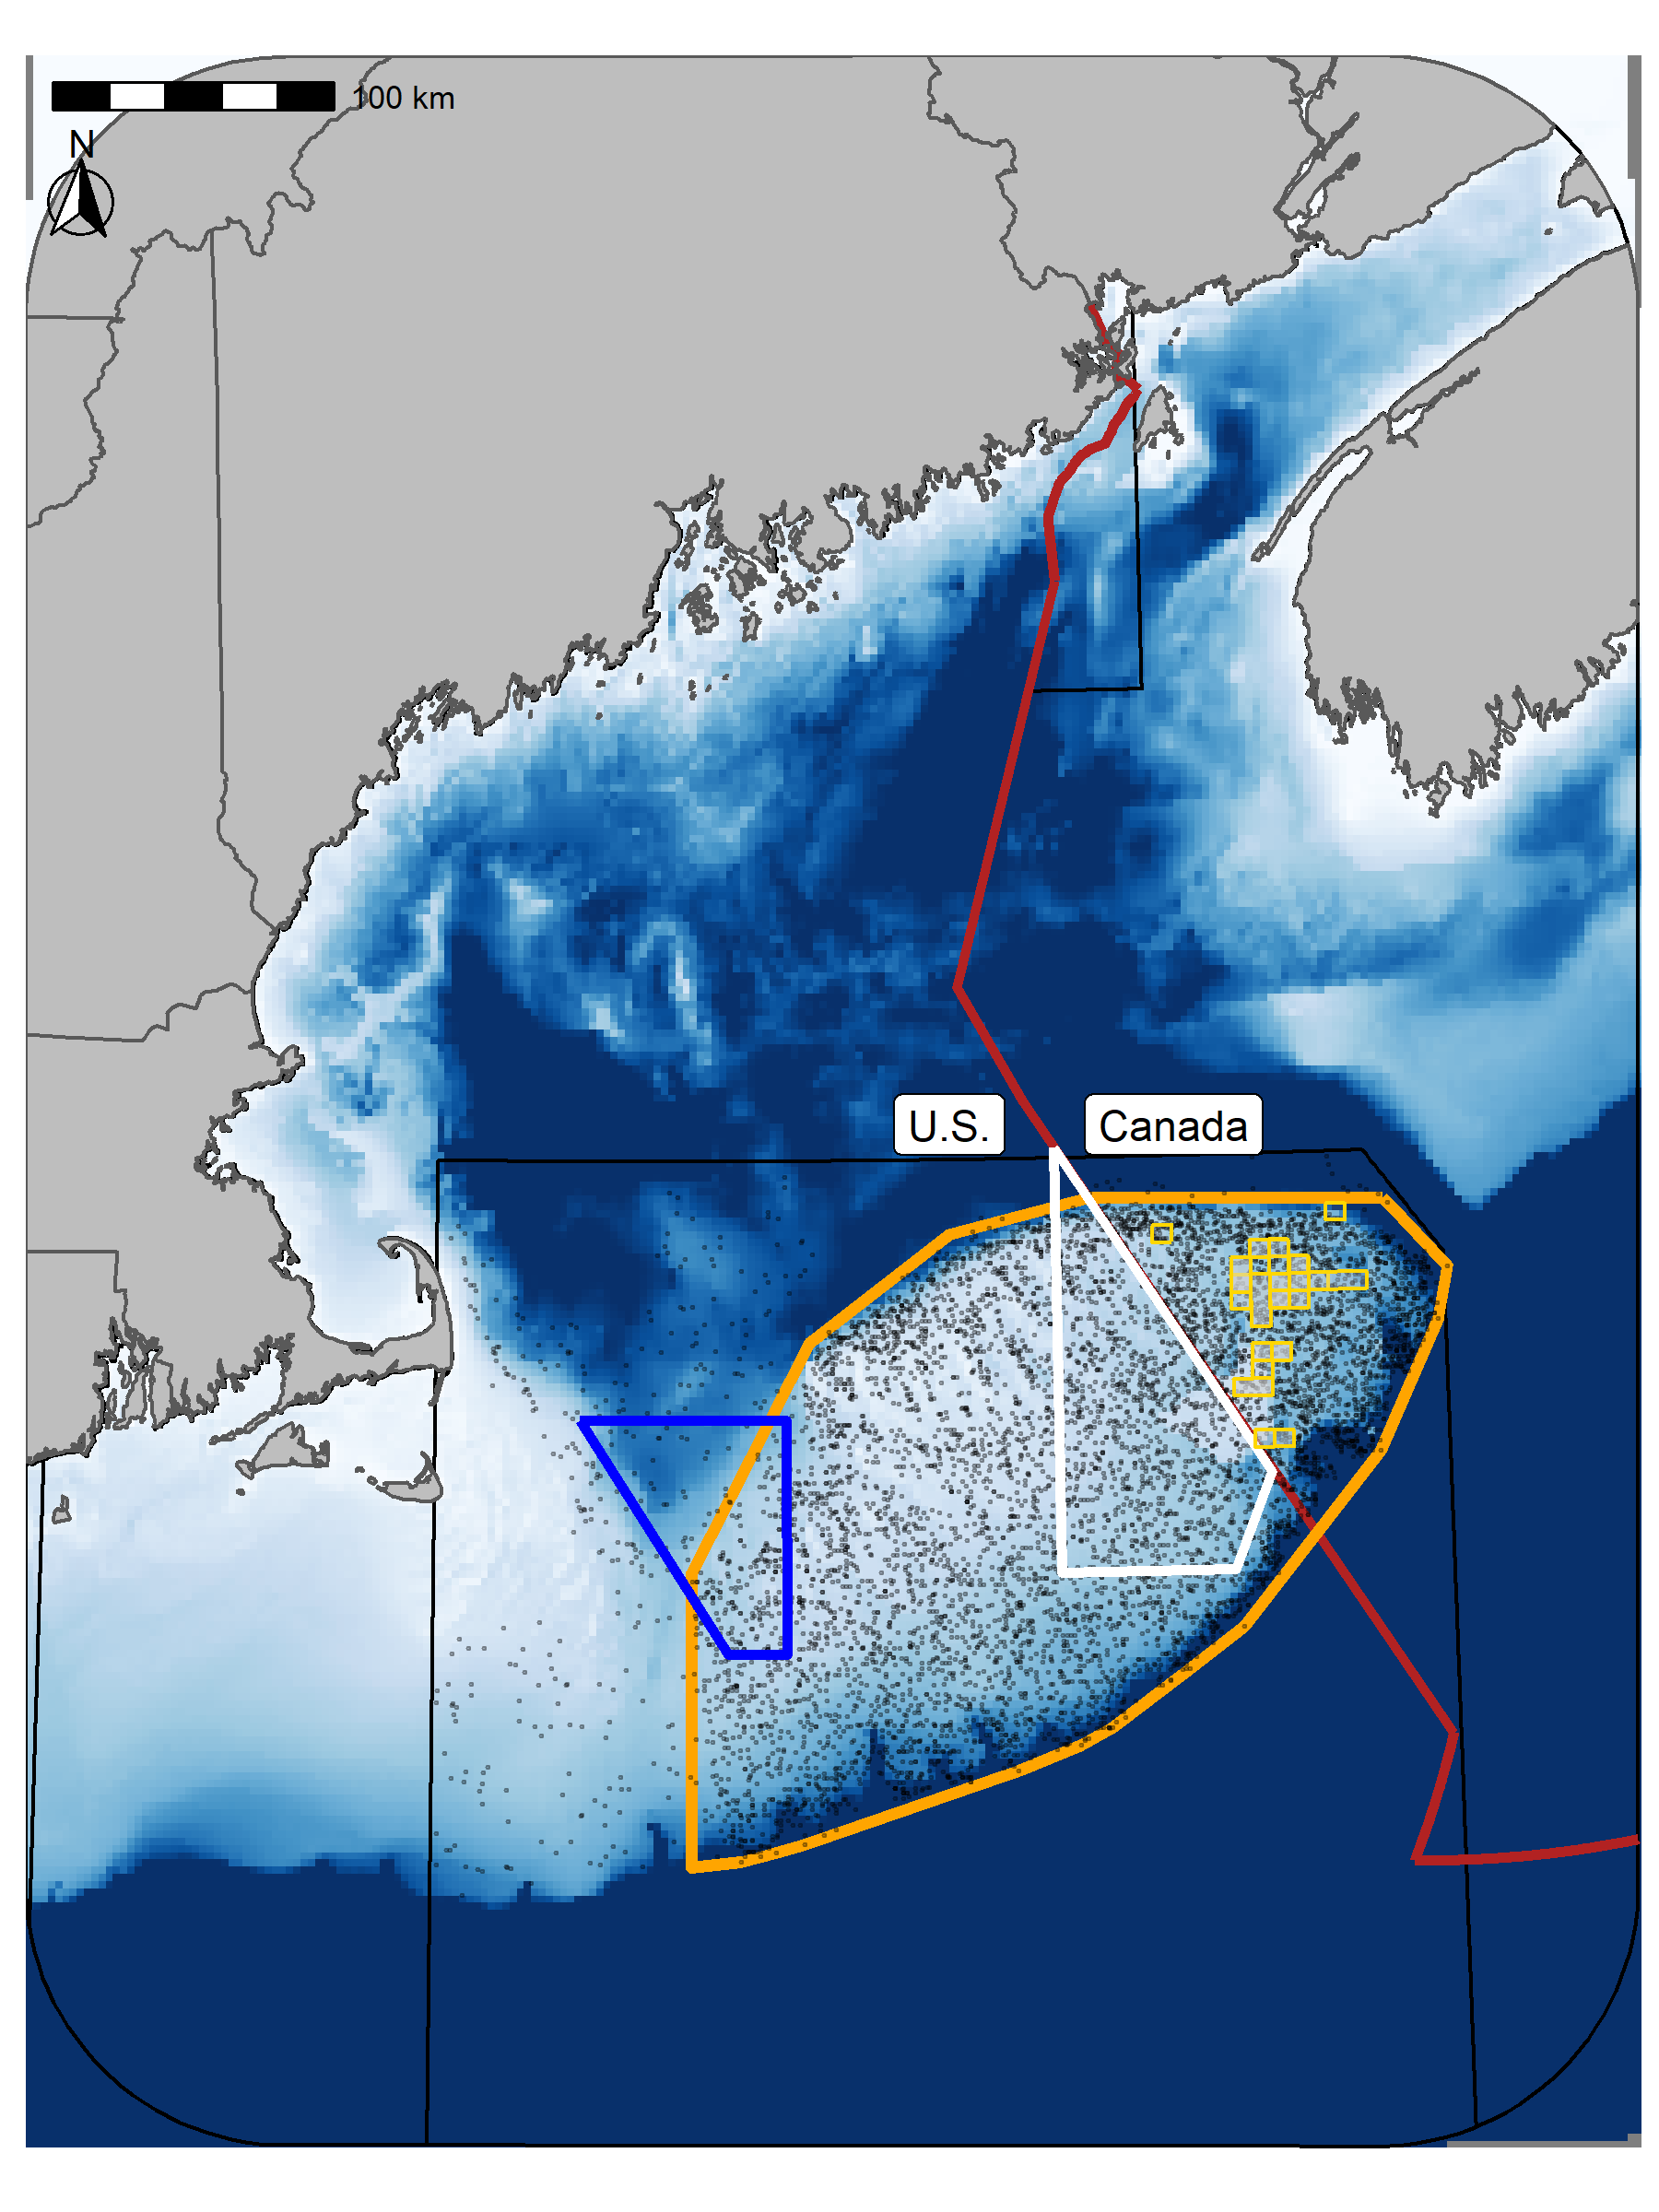
\includegraphics[width=1\linewidth]{D:/Github/Paper_2_SDMs/Results/Figures/GB_overview} \caption{Georges Bank (GB) study area.  Points represent the sample locations for each of the three surveys and the orange outline represents the core region of GB included in these analyses (42,000 km²).  The red line delineates the Canadian exclusive economic zone (EEZ).}\label{fig:Overview}
\end{figure}

\clearpage
\begin{figure}
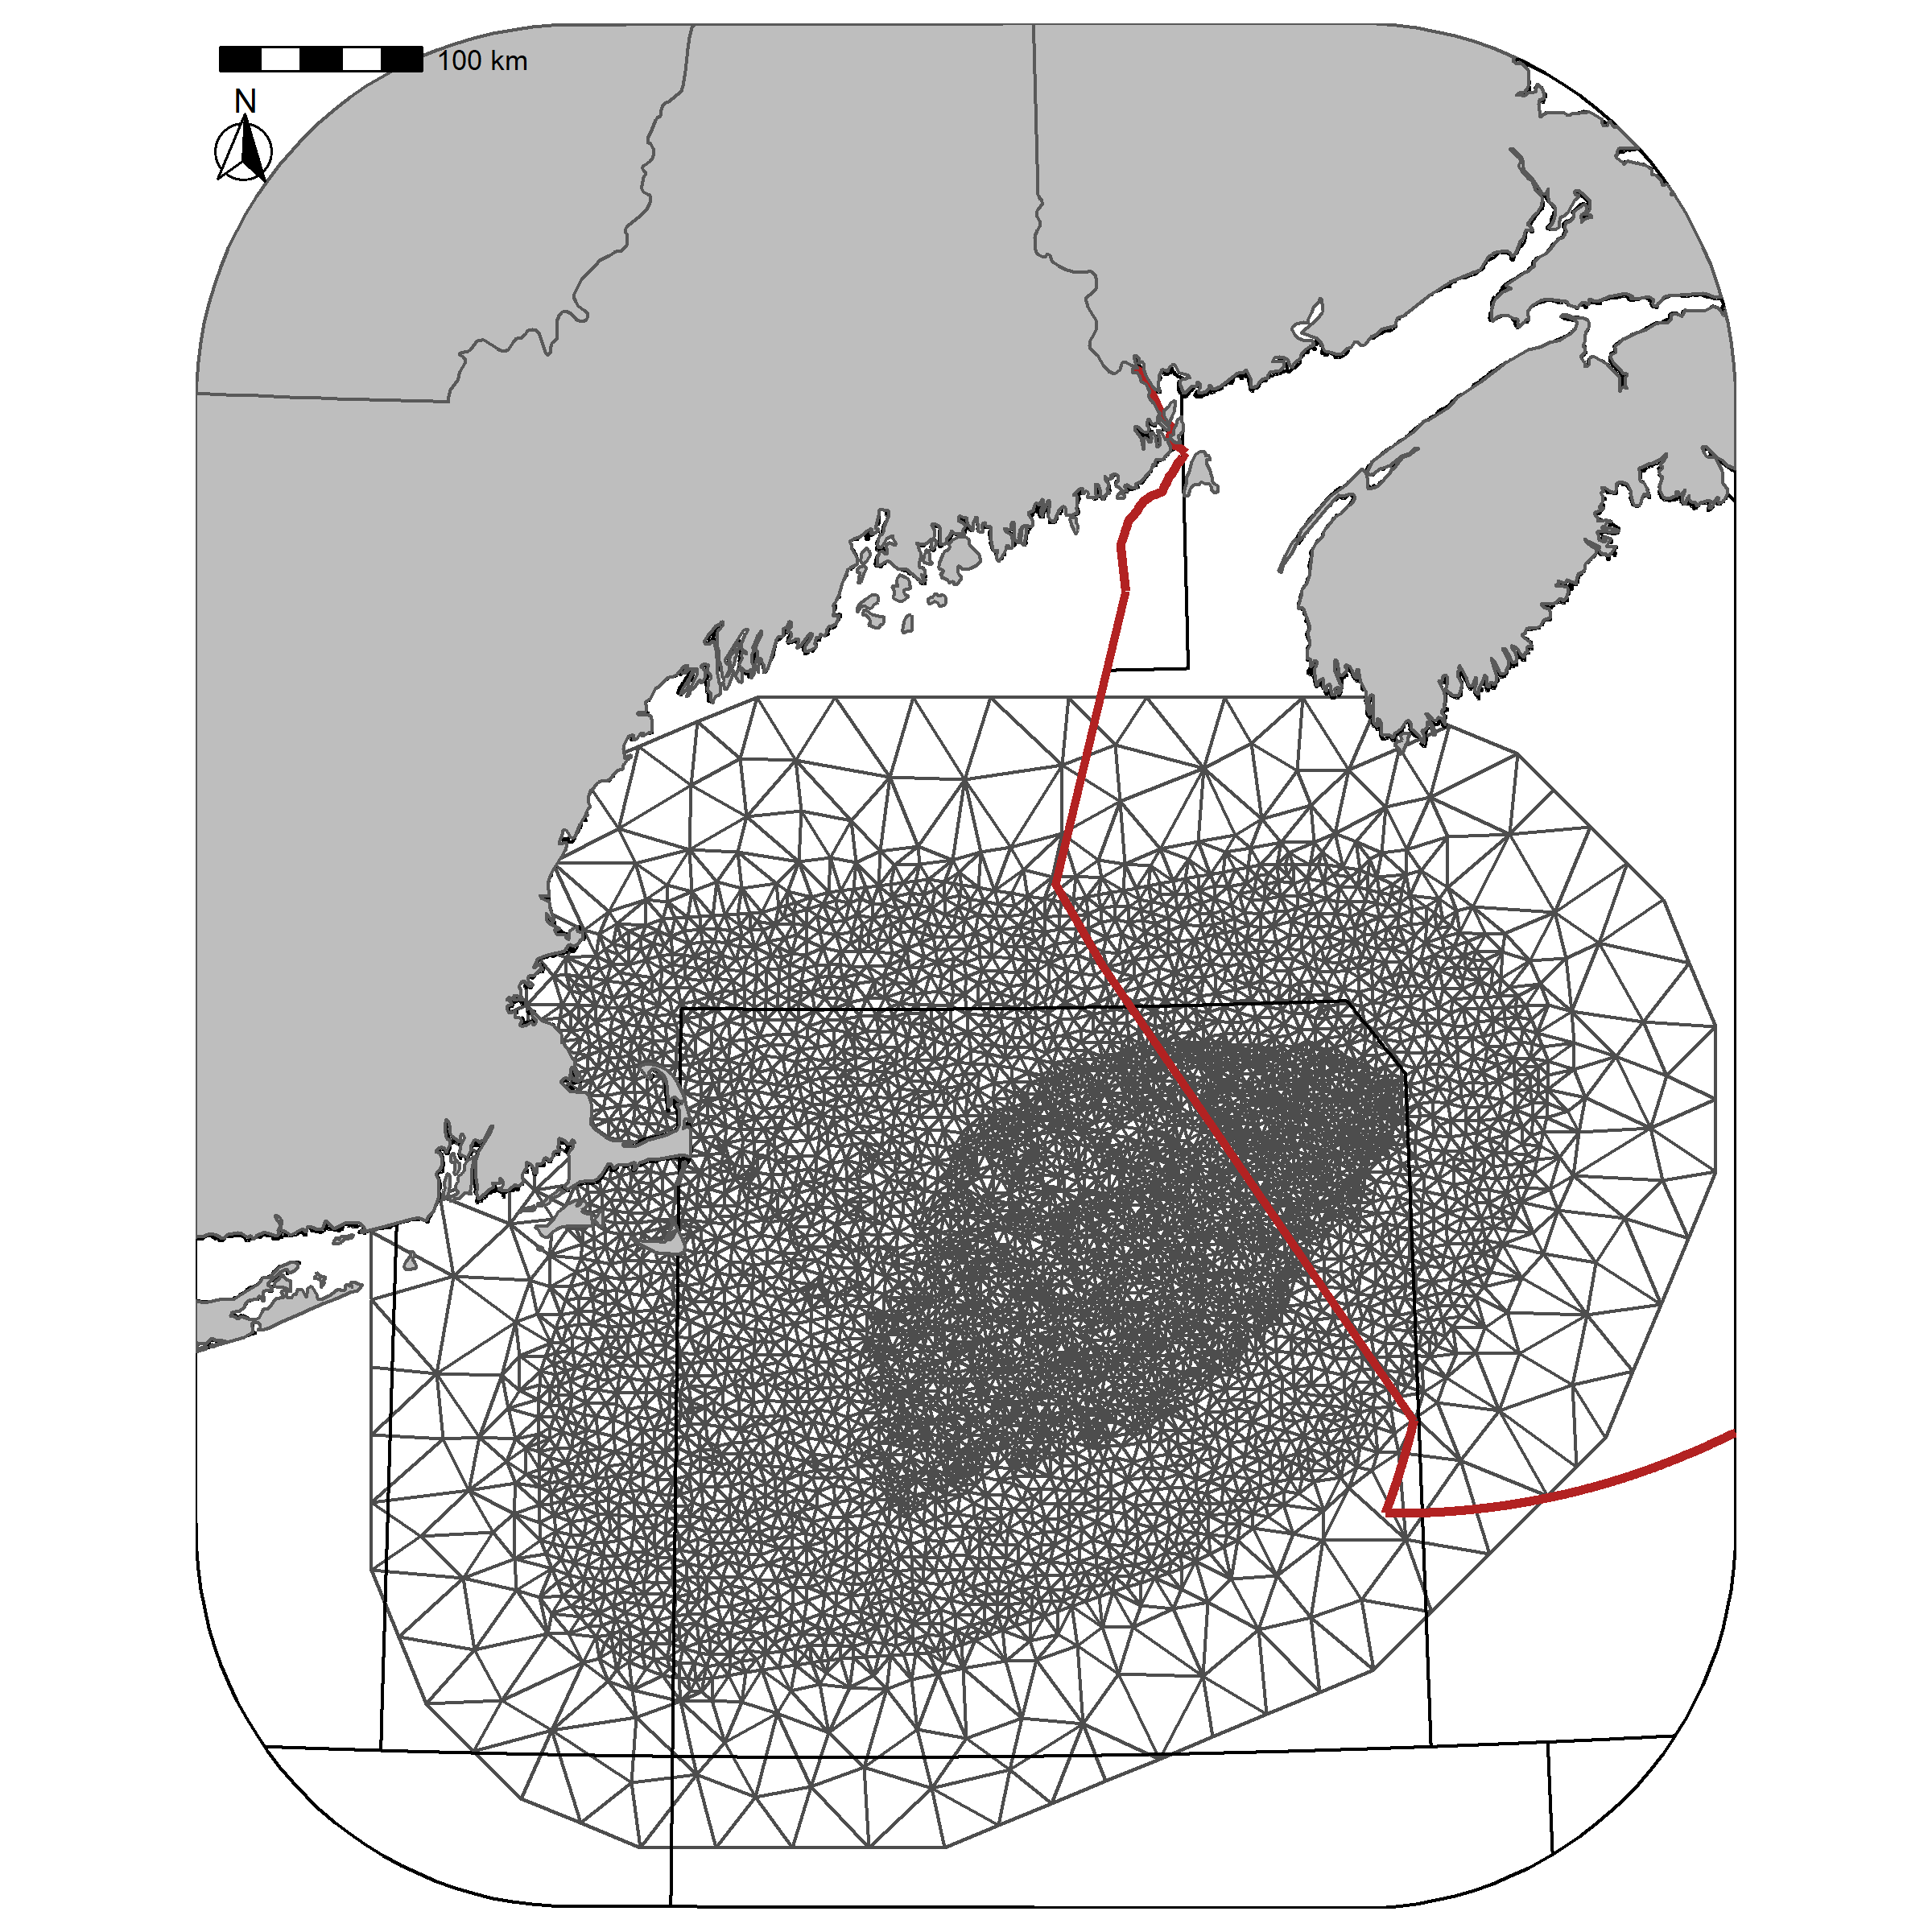
\includegraphics[width=1\linewidth]{D:/Github/Paper_2_SDMs/Results/Figures/mesh} \caption{Delaunay triangular mesh used for the analyses. The mesh contains 6610 vertices. The red line delineates the Canadian exclusive economic zone (EEZ).}\label{fig:Mesh}
\end{figure}

\begin{landscape}
\newpage
\begin{figure}
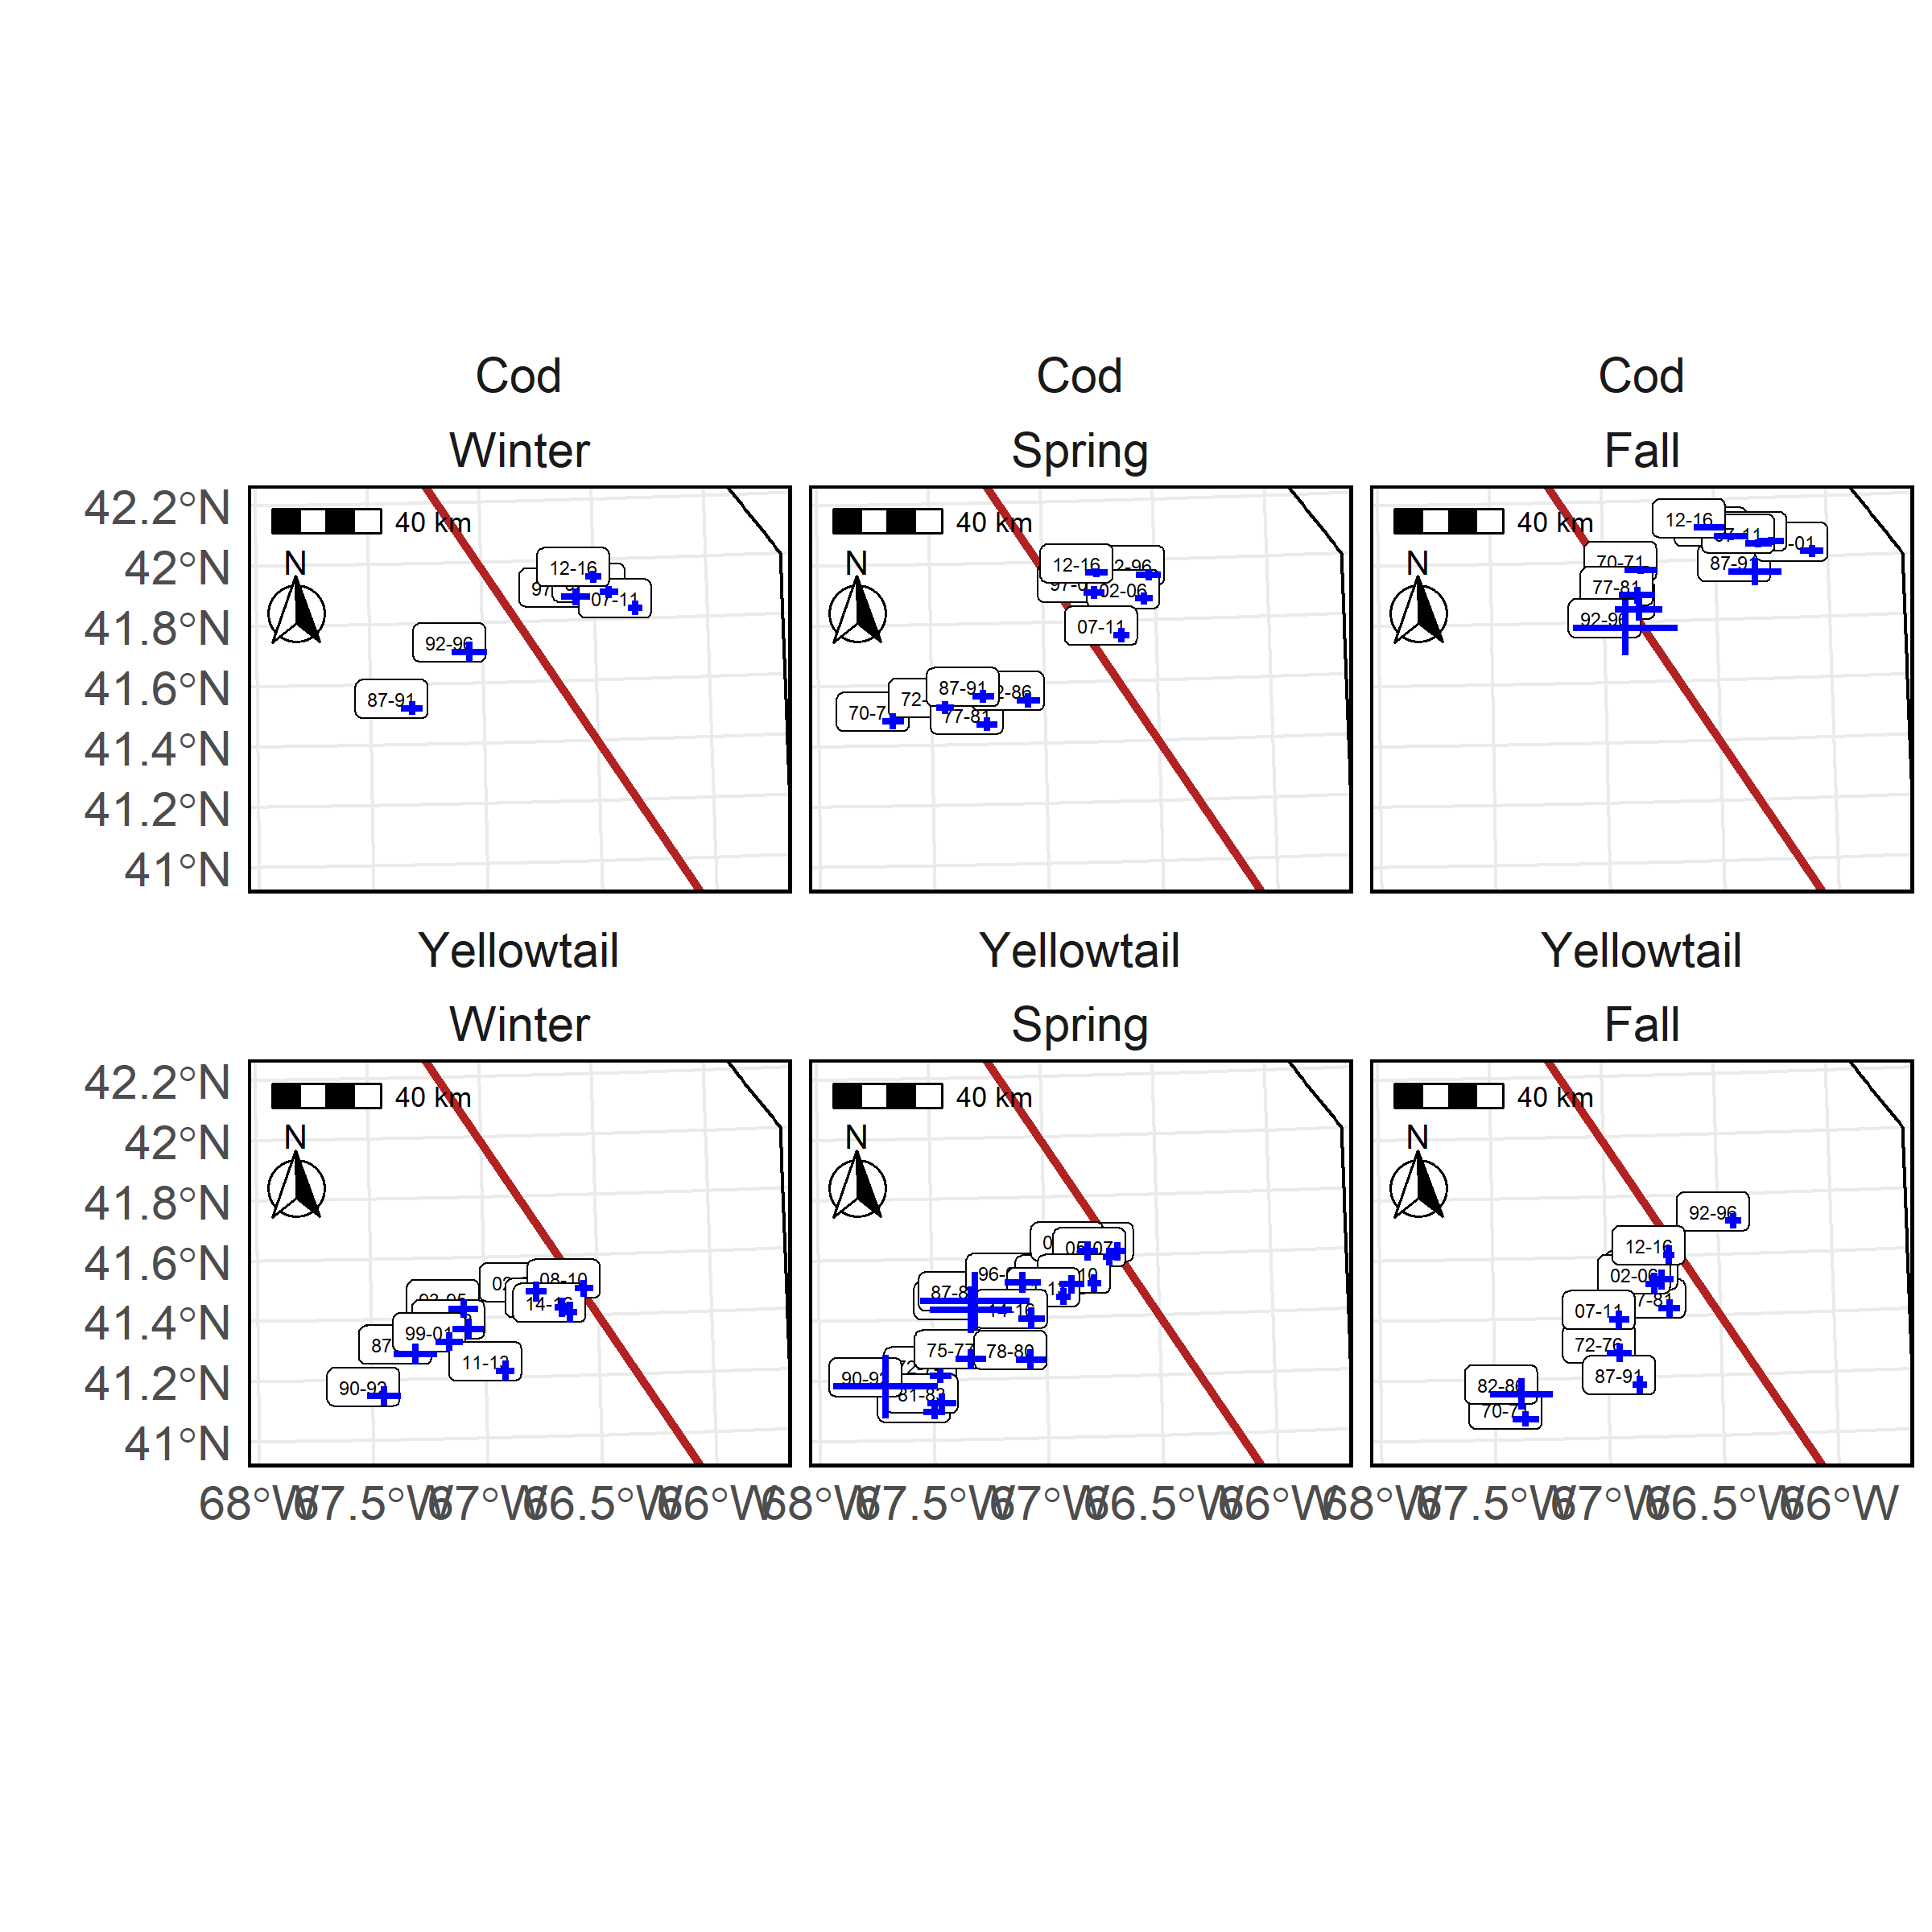
\includegraphics[width=1\linewidth]{D:/Github/Paper_2_SDMs/Results/Figures/center_of_gravity} \caption{Center of Gravity (COG) for the core area (OP $\geq$ 0.75) of Atlantic Cod (top panel) and Yellowtail Flounder (bottom panels) in the Winter (left), Spring (center), and Fall (right) using the final models.  Blue lines indicate ±3 standard deviation units from the mean COG. Labels indicate the years associated with each era and the red line is border between the U.S. and Canada.}\label{fig:cog-hep}
\end{figure}

\newpage
\begin{figure}
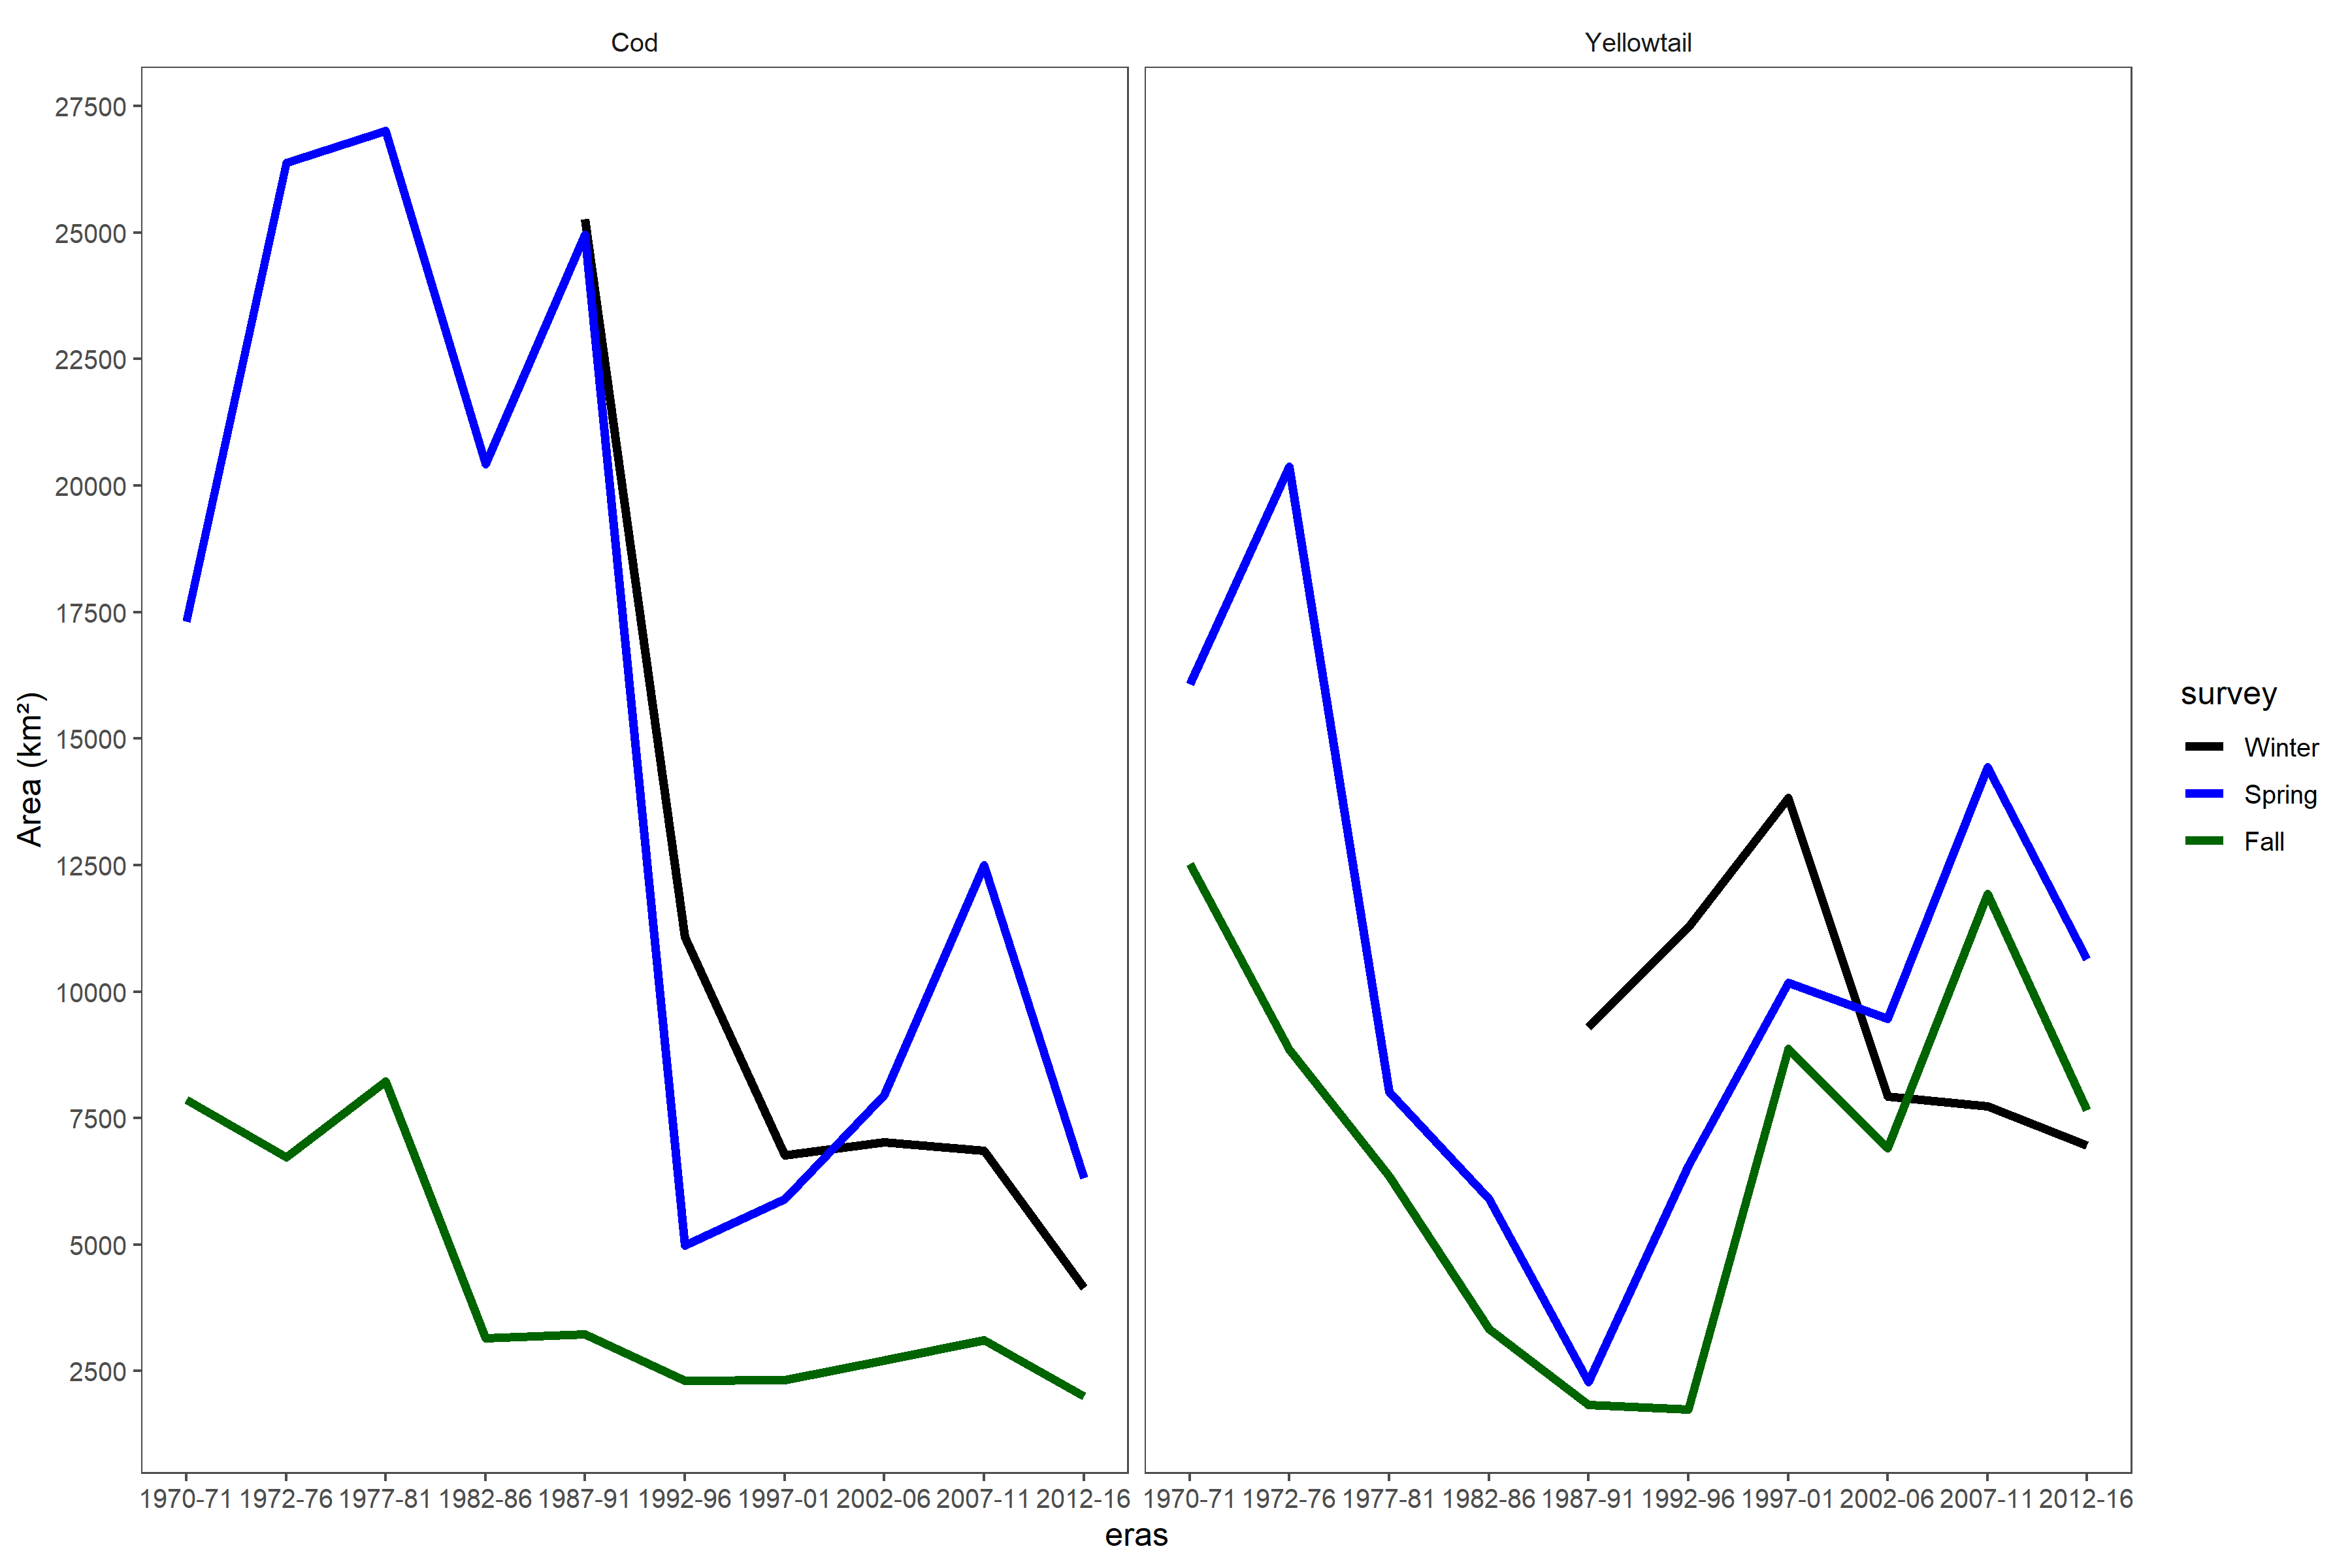
\includegraphics[width=1\linewidth]{D:/Github/Paper_2_SDMs/Results/Figures/Area_ts_high} \caption{Time series of the size of the core area (OP $\geq$ 0.75) on GB for each of the three seasons using the final models.  The Atlantic Cod time series is on the left and the Yellowtail Flounder on the right.  The black line represents the Winter trend, the blue line is the Spring trend, and the green line is the Fall trend.  }\label{fig:area-hep}
\end{figure}

\newpage
\begin{figure}
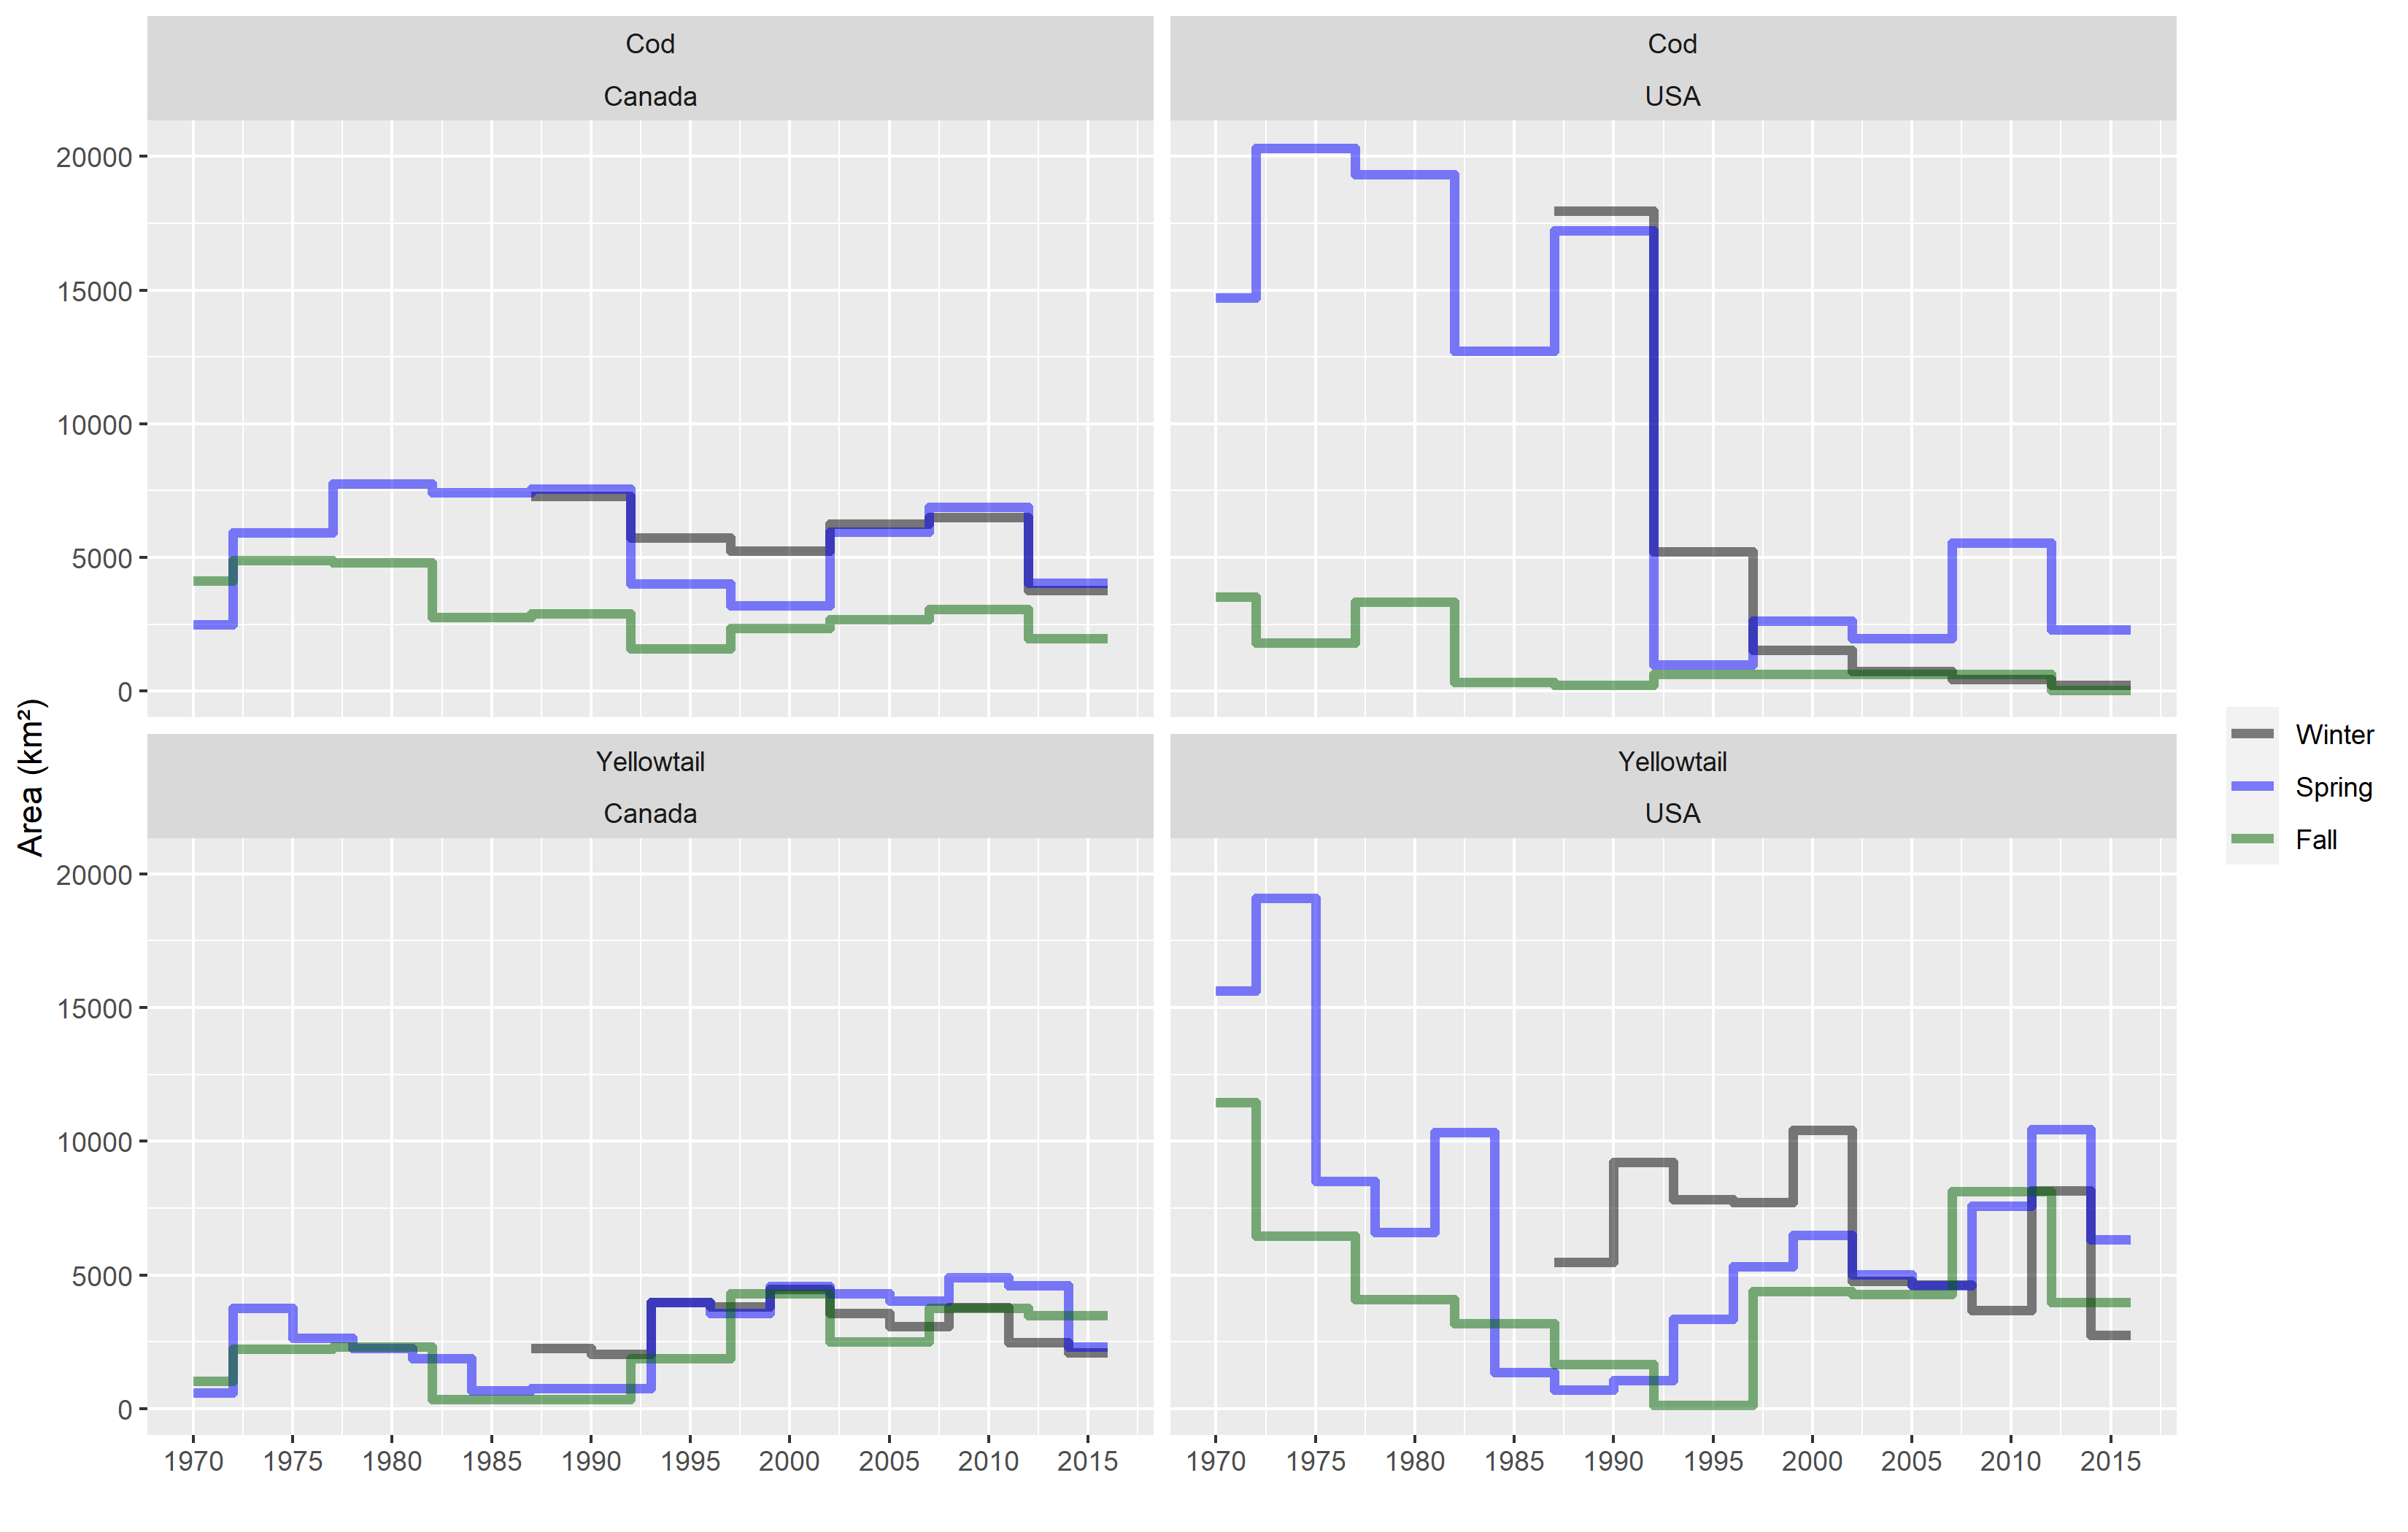
\includegraphics[width=1\linewidth]{D:/Github/Paper_2_SDMs/Results/Figures/Area_can_vs_us_ts_high} \caption{Time series of the size of the core area (OP $\geq$ 0.75) on for each of the three seasons in Canada and the U.S..  The Atlantic Cod time series is in the top row and Yellowtail Flounder in the bottom row, Canada is on the left and U.S. is on the right.  The black line represents the Winter trend, the blue line is the Spring trend, and the green line is the Fall trend.  }\label{fig:area-can-vs-us-hep}
\end{figure}

\newpage
\begin{figure}
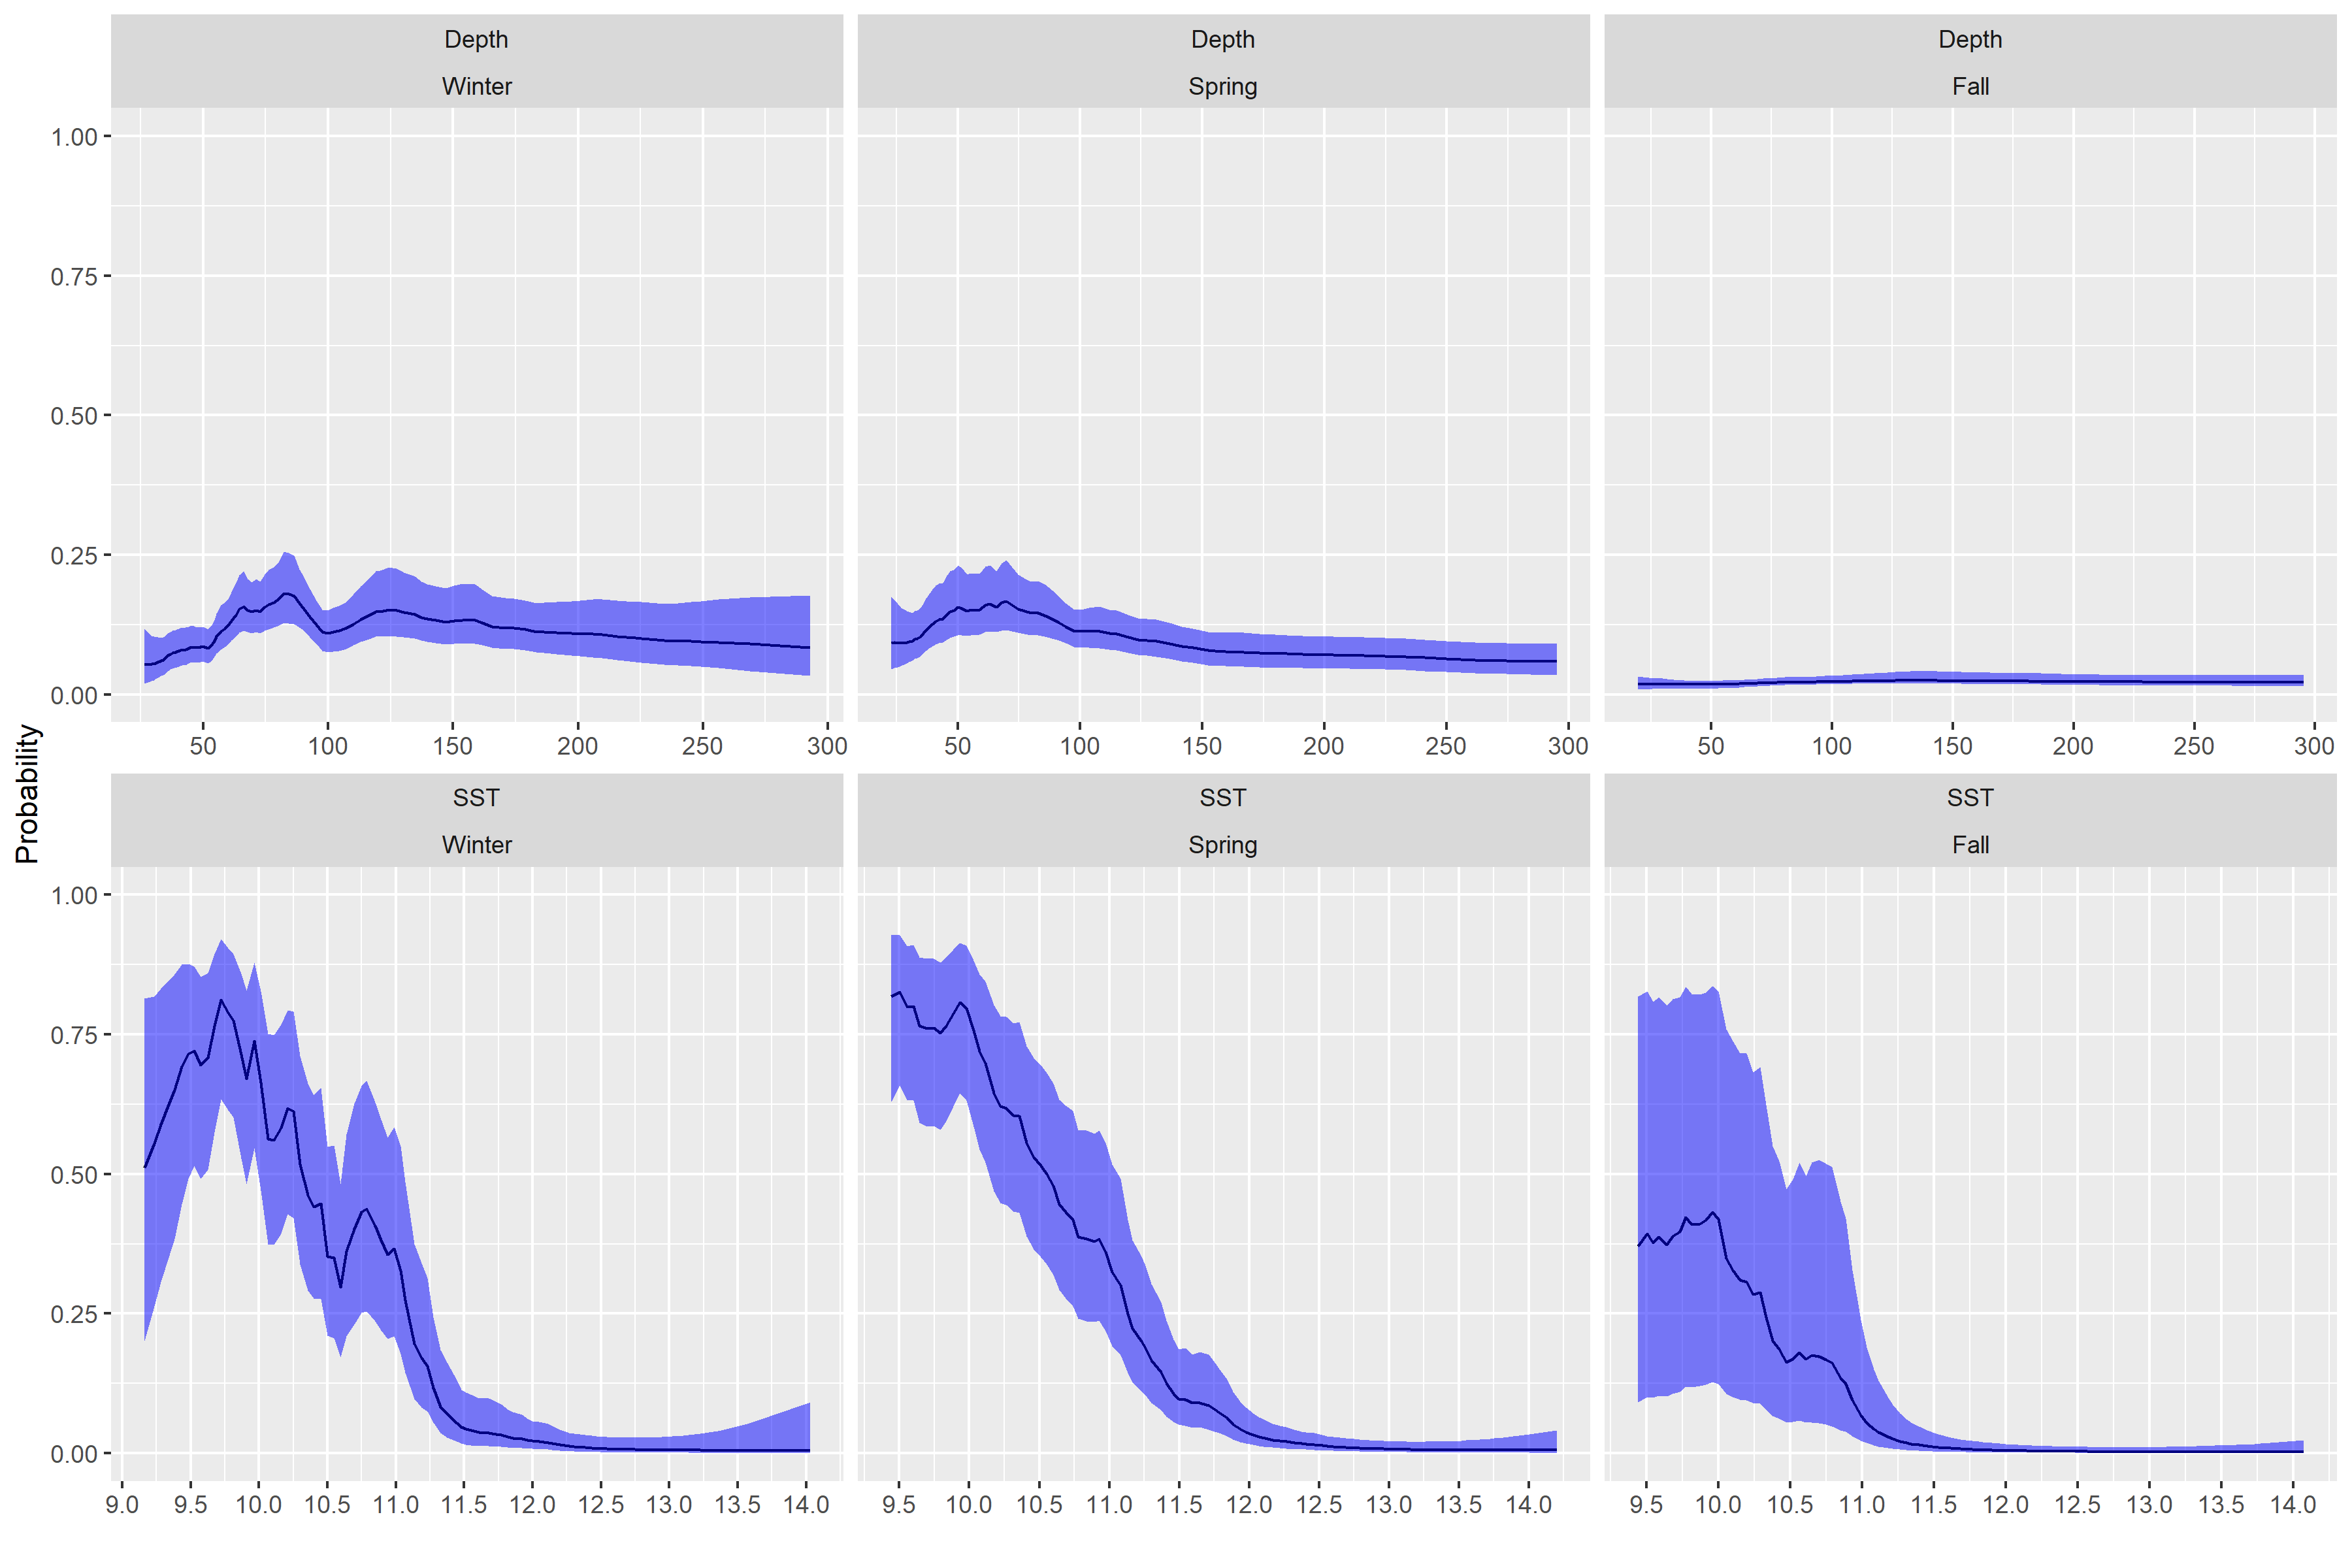
\includegraphics[width=1\linewidth]{D:/Github/Paper_2_SDMs/Results/Figures/Cod_fixed_effects} \caption{Environmental covariate effects for Atlantic Cod for each season, top row is the Dep covariate effect, bottom row is the SST effect. Results have been transformed to the probability scale and the blue shaded region represents the 95\% credible interval.}\label{fig:cod-fe}
\end{figure}

\newpage
\begin{figure}
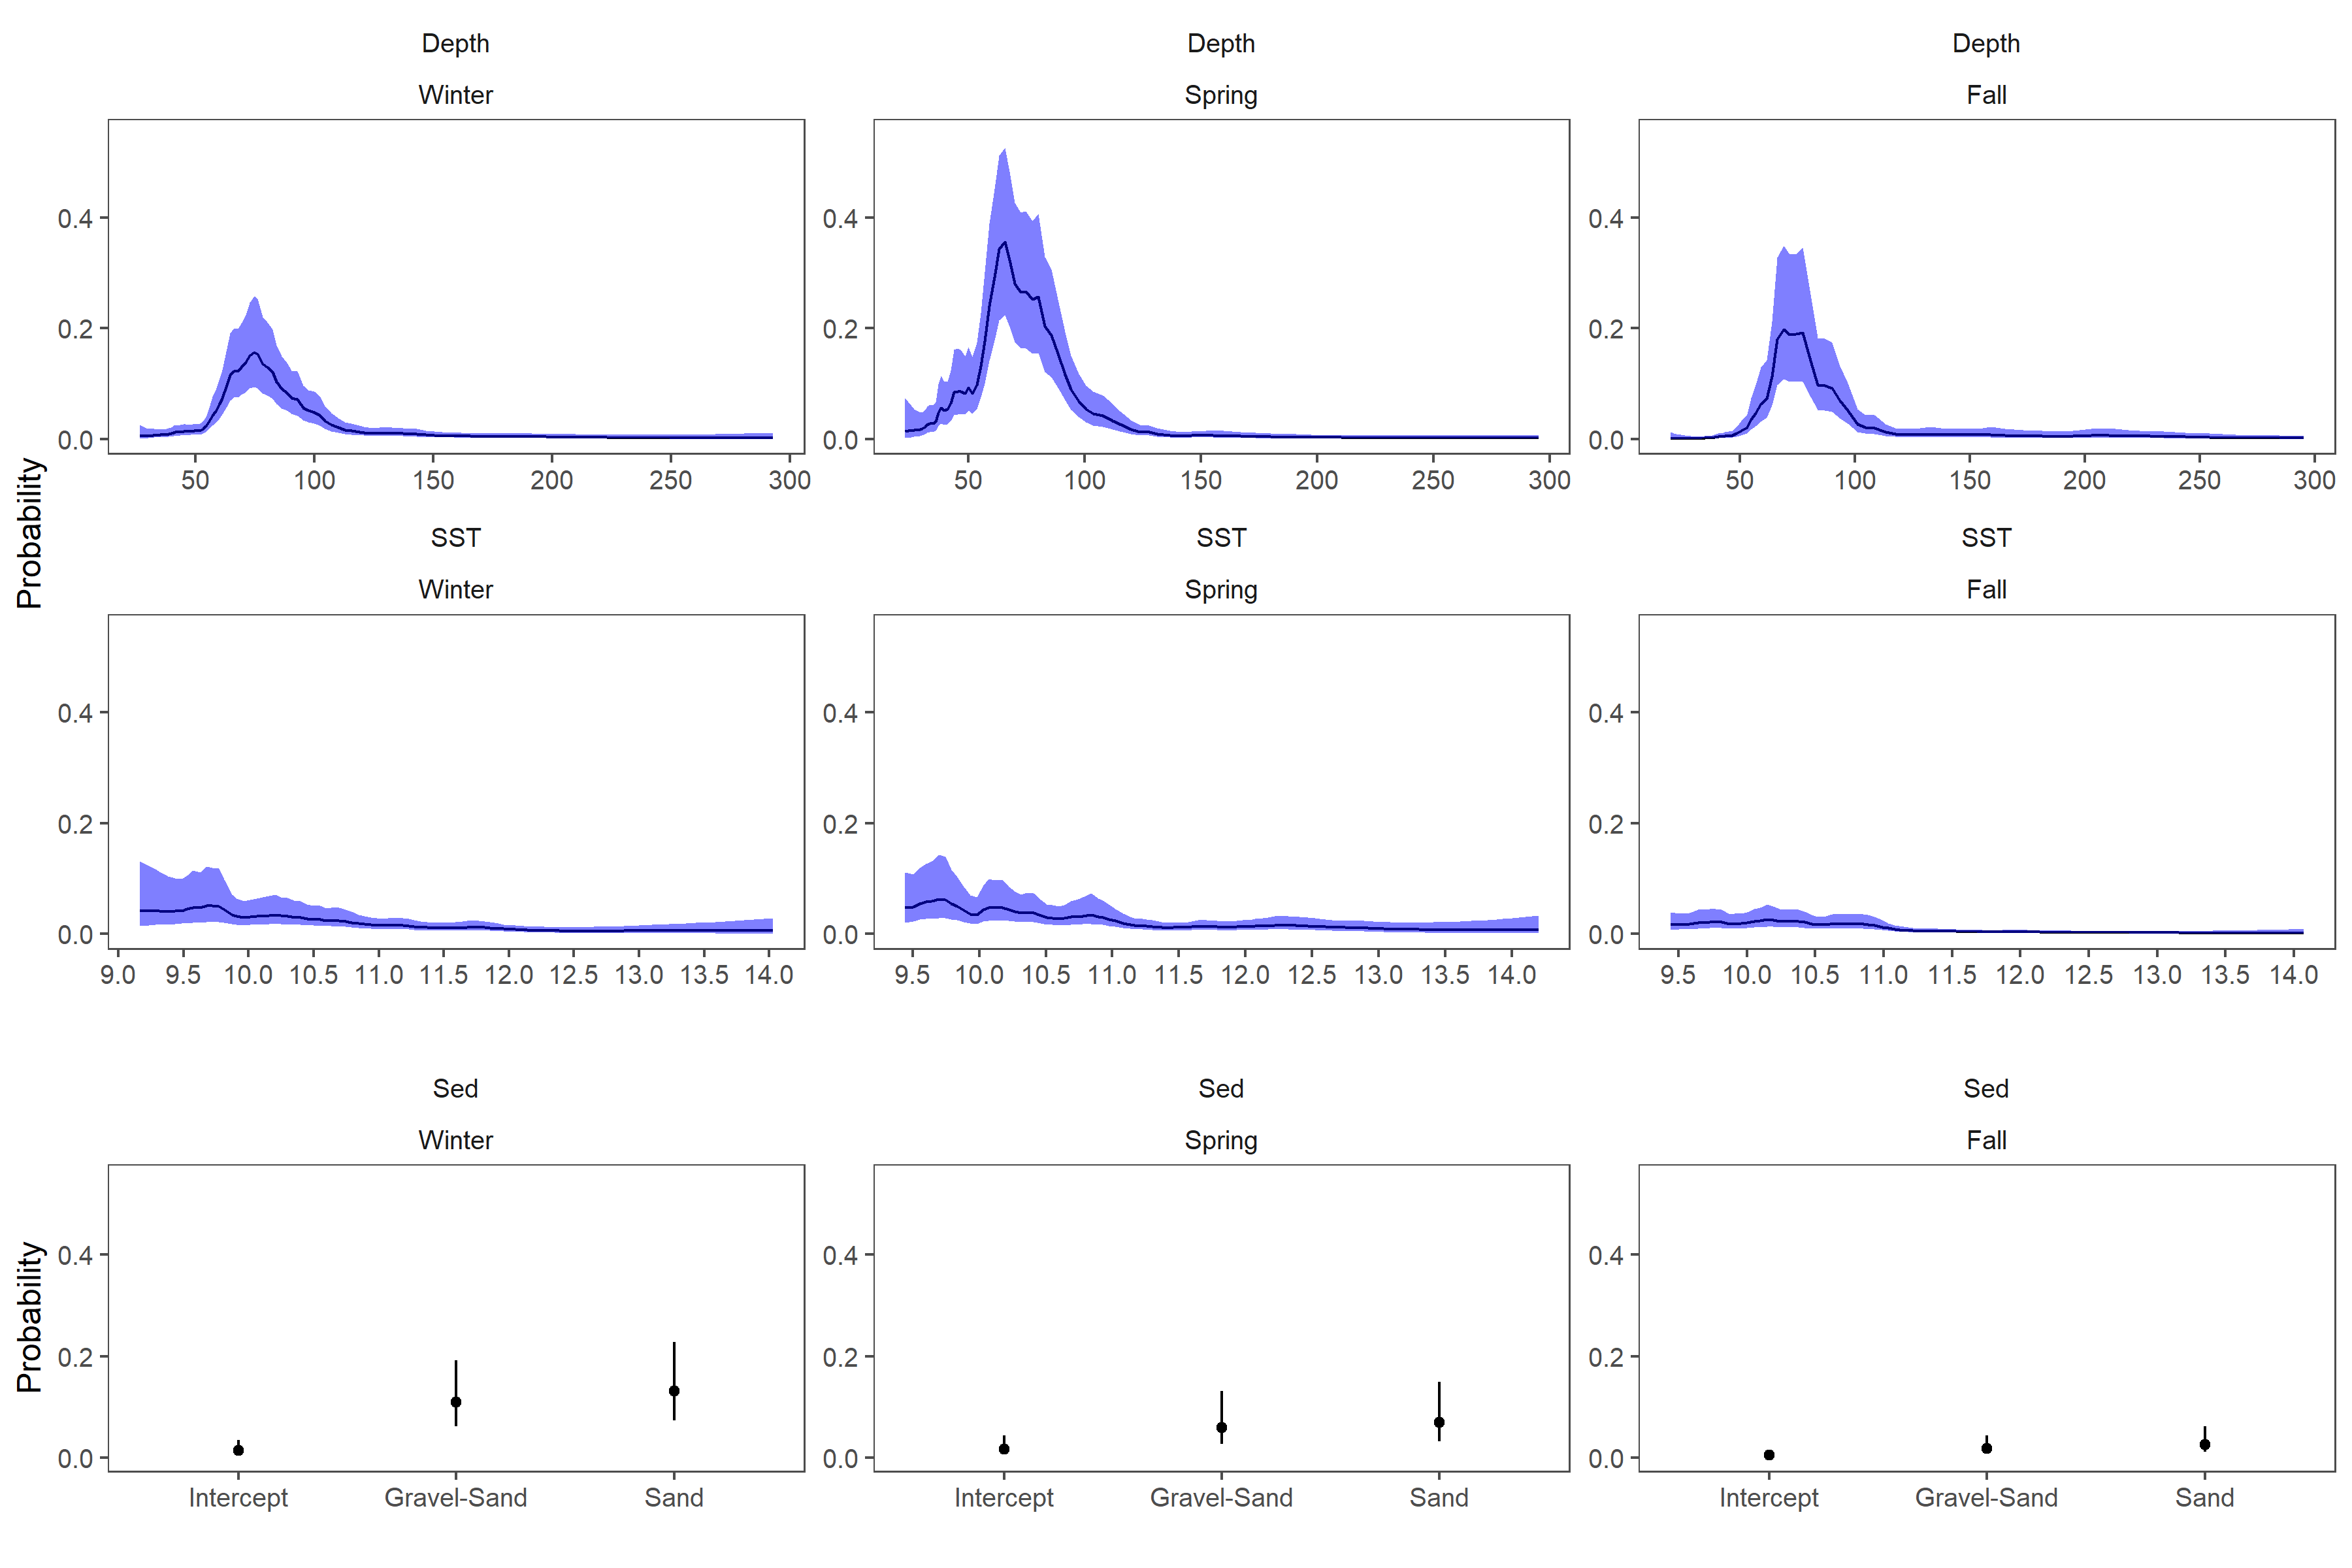
\includegraphics[width=1\linewidth]{D:/Github/Paper_2_SDMs/Results/Figures/yt_fixed_effects} \caption{Environmental covariate effects for Yellowtail Flounder for each season, the top row is the Dep covariate effect, middle row is the SST effect, and the bottom row is the Sed effect. Results have been transformed to the probability scale, and the blue shaded region and the error bars represent the 95\% credible intervals. The Winter and Spring results use a 3 year random field while the Fall results are for the 5 year random field model.}\label{fig:yt-fe}
\end{figure}

\clearpage

\begin{figure}
\includegraphics[width=1\linewidth]{D:/Github/Paper_2_SDMs/Results/Figures/hyper_range_field_est} \caption{Decorrelation range estimate with 95\% credible intervals for each season.}\label{fig:hyper-range-var-est}
\end{figure}

\clearpage

\begin{figure}
\includegraphics[width=1\linewidth]{D:/Github/Paper_2_SDMs/Results/Figures/hyper_sd_field_est} \caption{Standard Deviation of the field with 95\% credible intervals for each season.}\label{fig:hyper-sd-var-est}
\end{figure}

\newpage
\begin{figure}
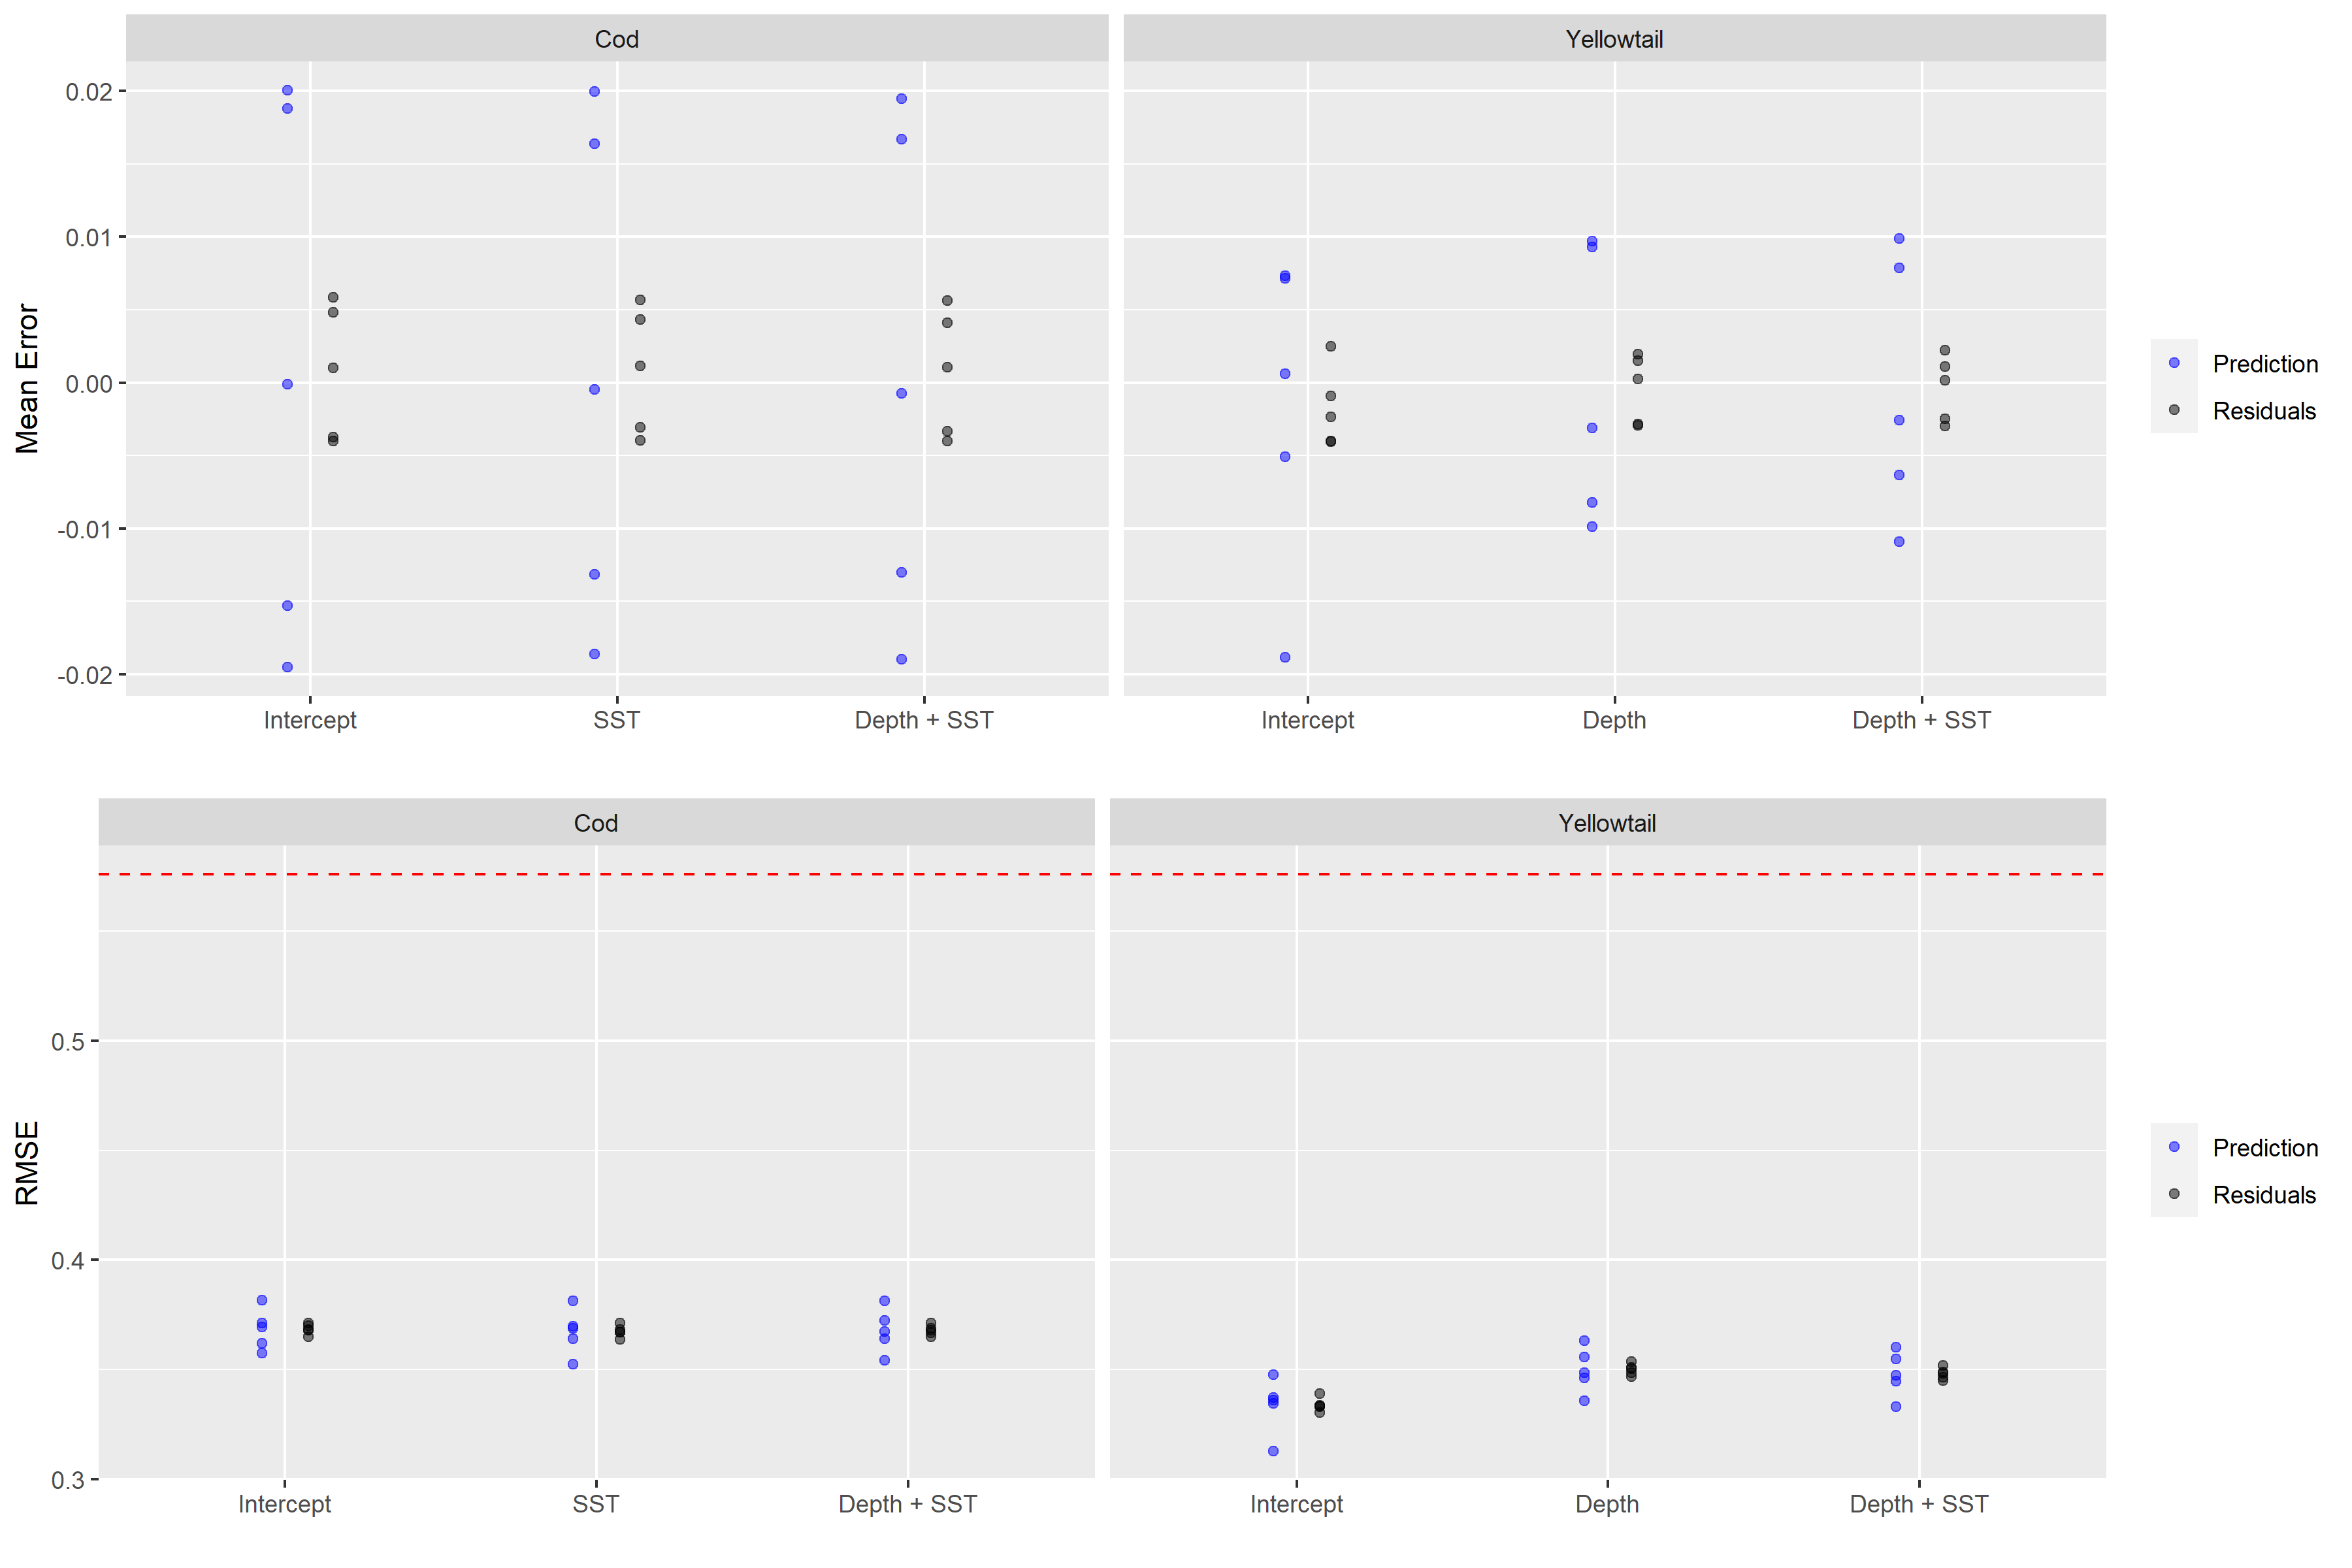
\includegraphics[width=1\linewidth]{D:/Github/Paper_2_SDMs/Results/Figures/cross_fold_validation} \caption{Results of five fold cross validation analyses. Top panels represents the mean error for each of the three covariate models tested for Atlantic Cod (using Winter data) and Yellowtail Flounder (using Spring data). Blue points represent the prediction error from the testing dataset, while the black points are the residuals from the training dataset. The bottom panels are the RMSE for these models.  The red dashed line represents the RMSE for randomly generated data and represents the RMSE for a model with no predictive ability. All models use the 5 year random field due to computational constraints.}\label{fig:folds}
\end{figure}

\newpage
\begin{figure}
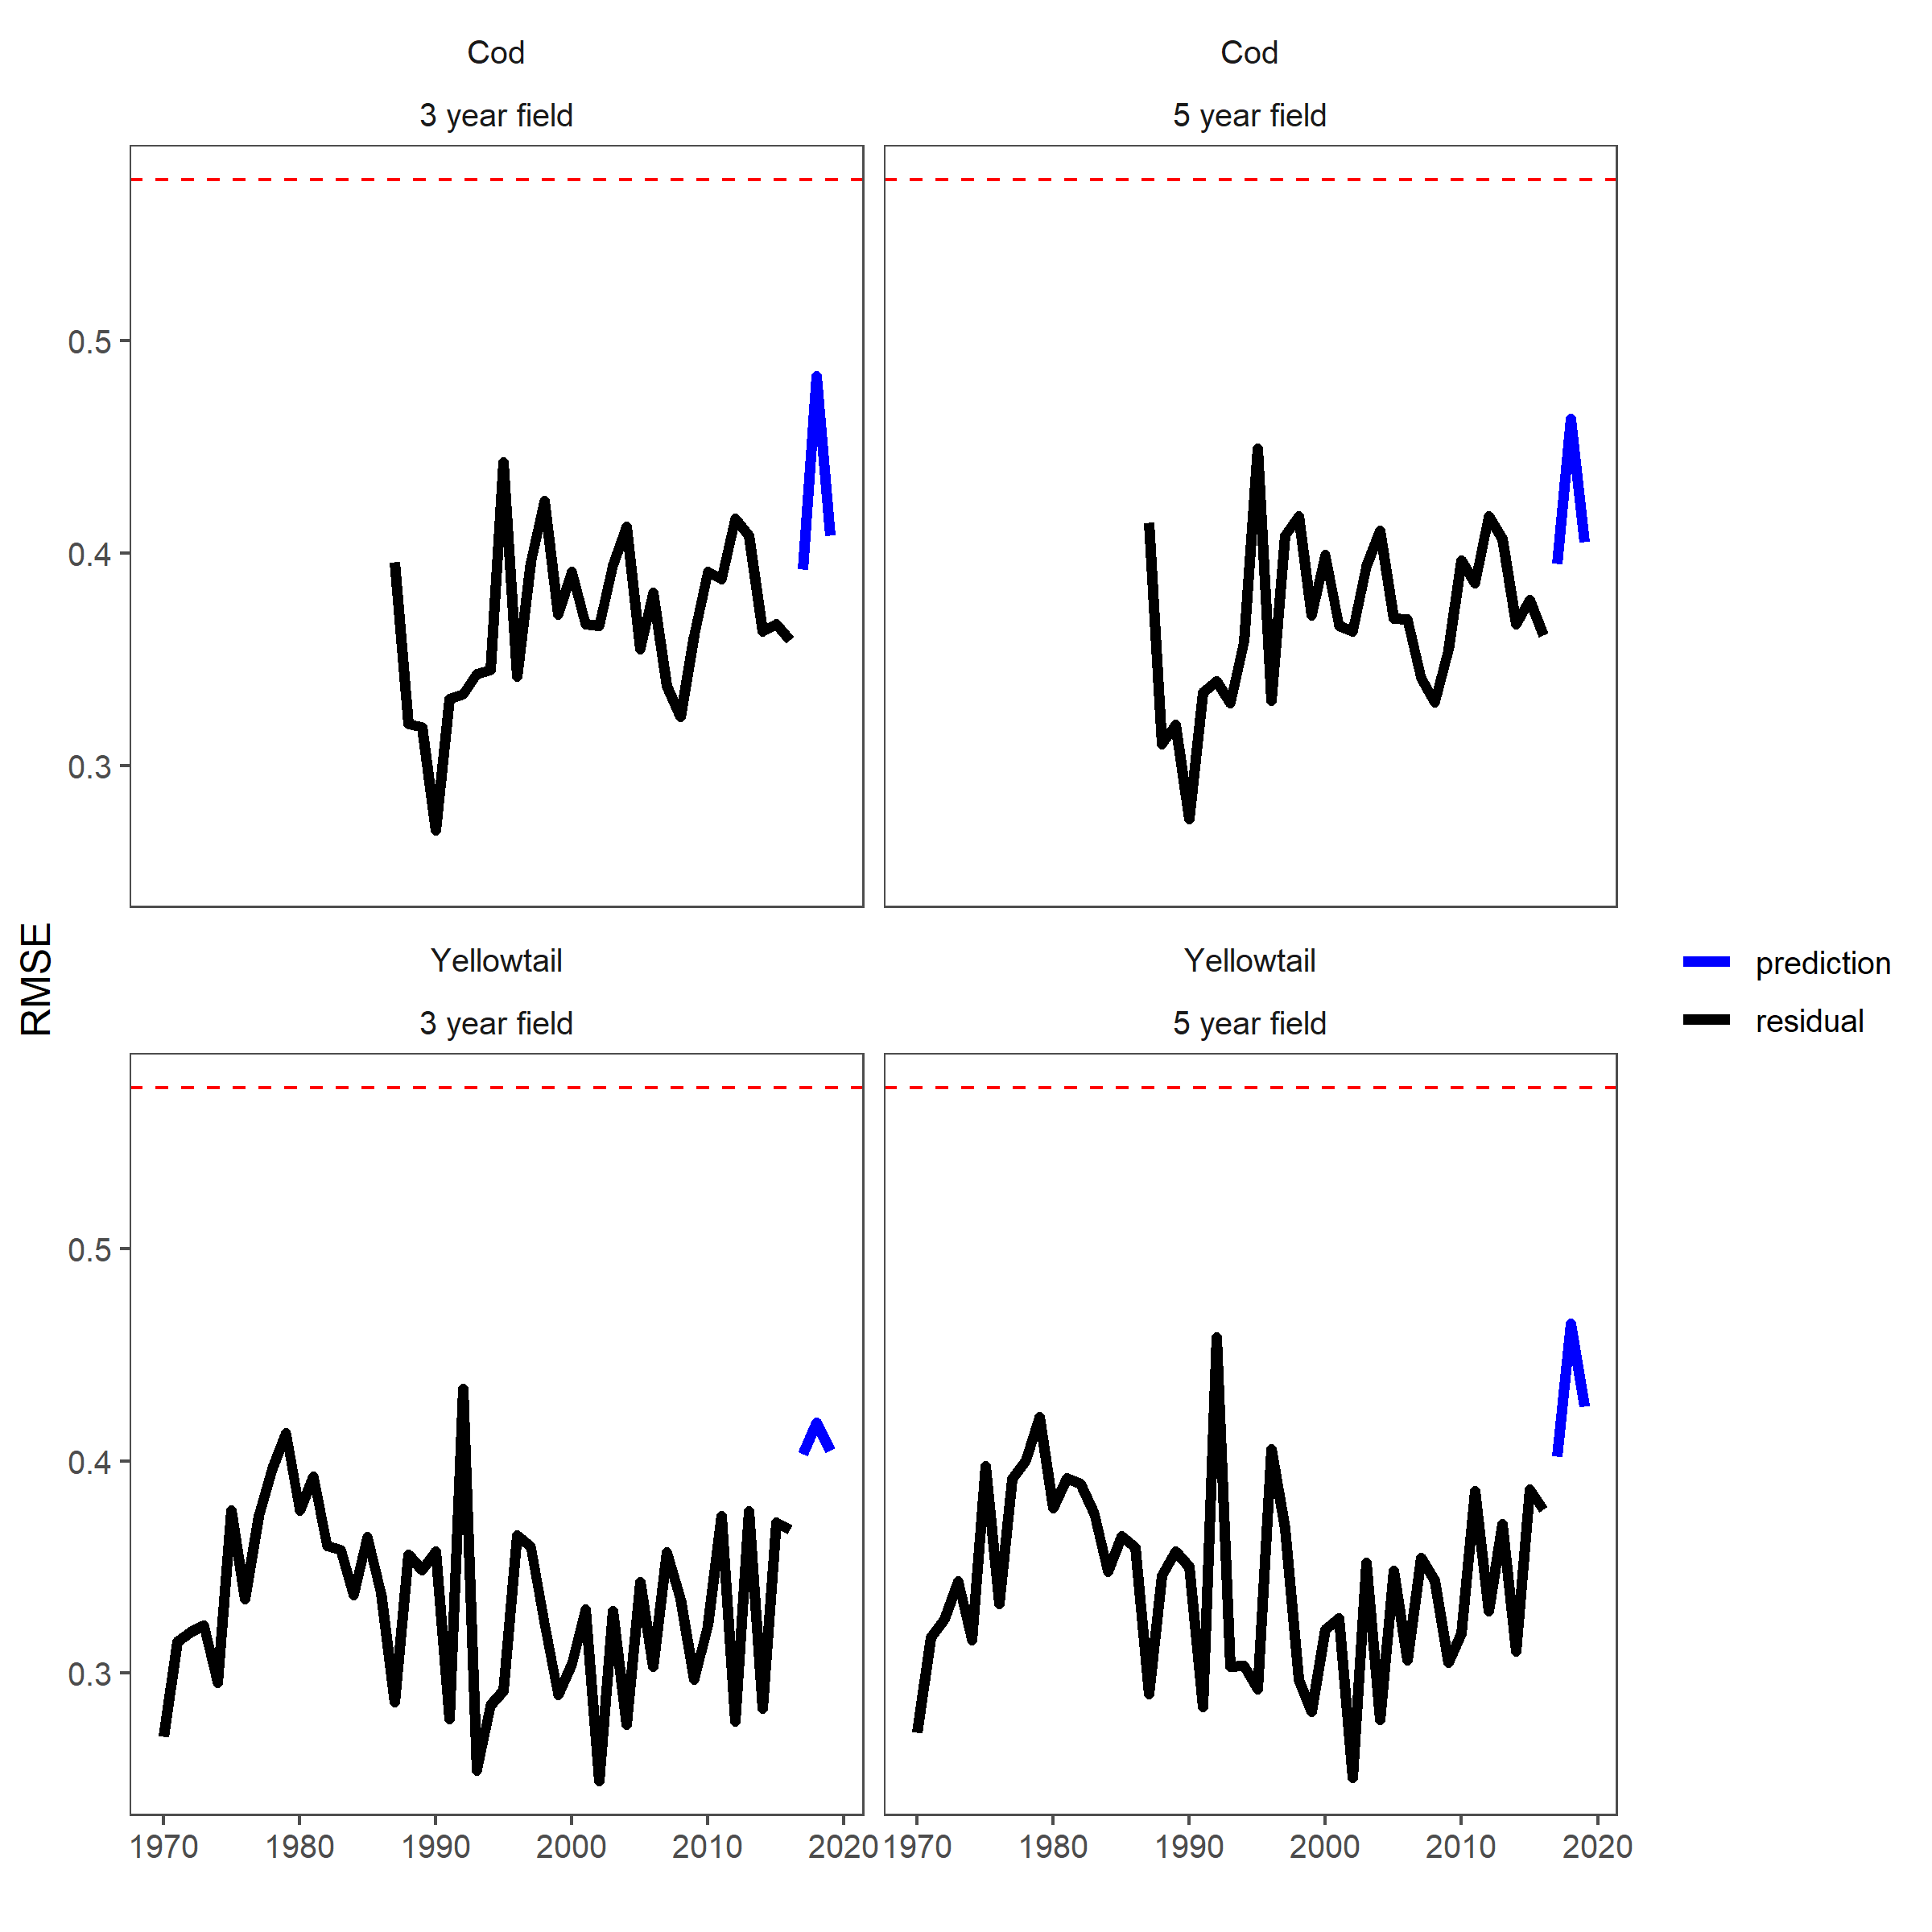
\includegraphics[width=1\linewidth]{D:/Github/Paper_2_SDMs/Results/Figures/prediction_2017_2019} \caption{The residual RMSE for the model is shown in black, while the blue lines represent the prediction RMSE for data in years 2017, 2018, and 2019. The models compared were a model with no covariates (intercept + random field) represented by the dashed line and a model which includes the additive SST and Dep covariates along with the random field represented by the solid line. Atlantic Cod results are in the top row and use a 5 year random field. Yellowtail Flounder results are in the bottom row and use a 3 year random field for the Winter and Spring and the 5 year random field for the Fall. The red dot-dash line represents the RMSE for randomly generated data and represents the RMSE for a model with no predictive ability.}\label{fig:pred-17-19}
\end{figure}

\end{landscape}

\newpage

\hypertarget{ref-sup}{%
\section{SUPPLEMENT 1}\label{ref-sup}}

\setcounter{table}{0}  \renewcommand{\thetable}{S\arabic{table}} \setcounter{figure}{0} \renewcommand{\thefigure}{S\arabic{figure}}

\newpage

\begin{figure}
\includegraphics[width=0.75\linewidth]{D:/Github/Paper_2_SDMs/Results/Figures/pca} \caption{Principal Component Analysis (PCA) results for the Winter, Spring, and Fall seasons using the retained environmental data and the 4 retained Princpal Components (PCs). The results for PC 1 and 2 for each season are on the top and the PC 3 and 4 results are on the bottom.  Left column are the results for Winter, middle column for Spring, and right column is for the Fall. The percentage of the variance explained by each PC is provided on the axes labels.  Points represent the score for each survey observation.  The loadings for each covariate in the analysis are shown by the length of their respective lines. PC scores greater than ± 3 units not shown.}\label{fig:PCA}
\end{figure}

\newpage

\clearpage
\begin{figure}
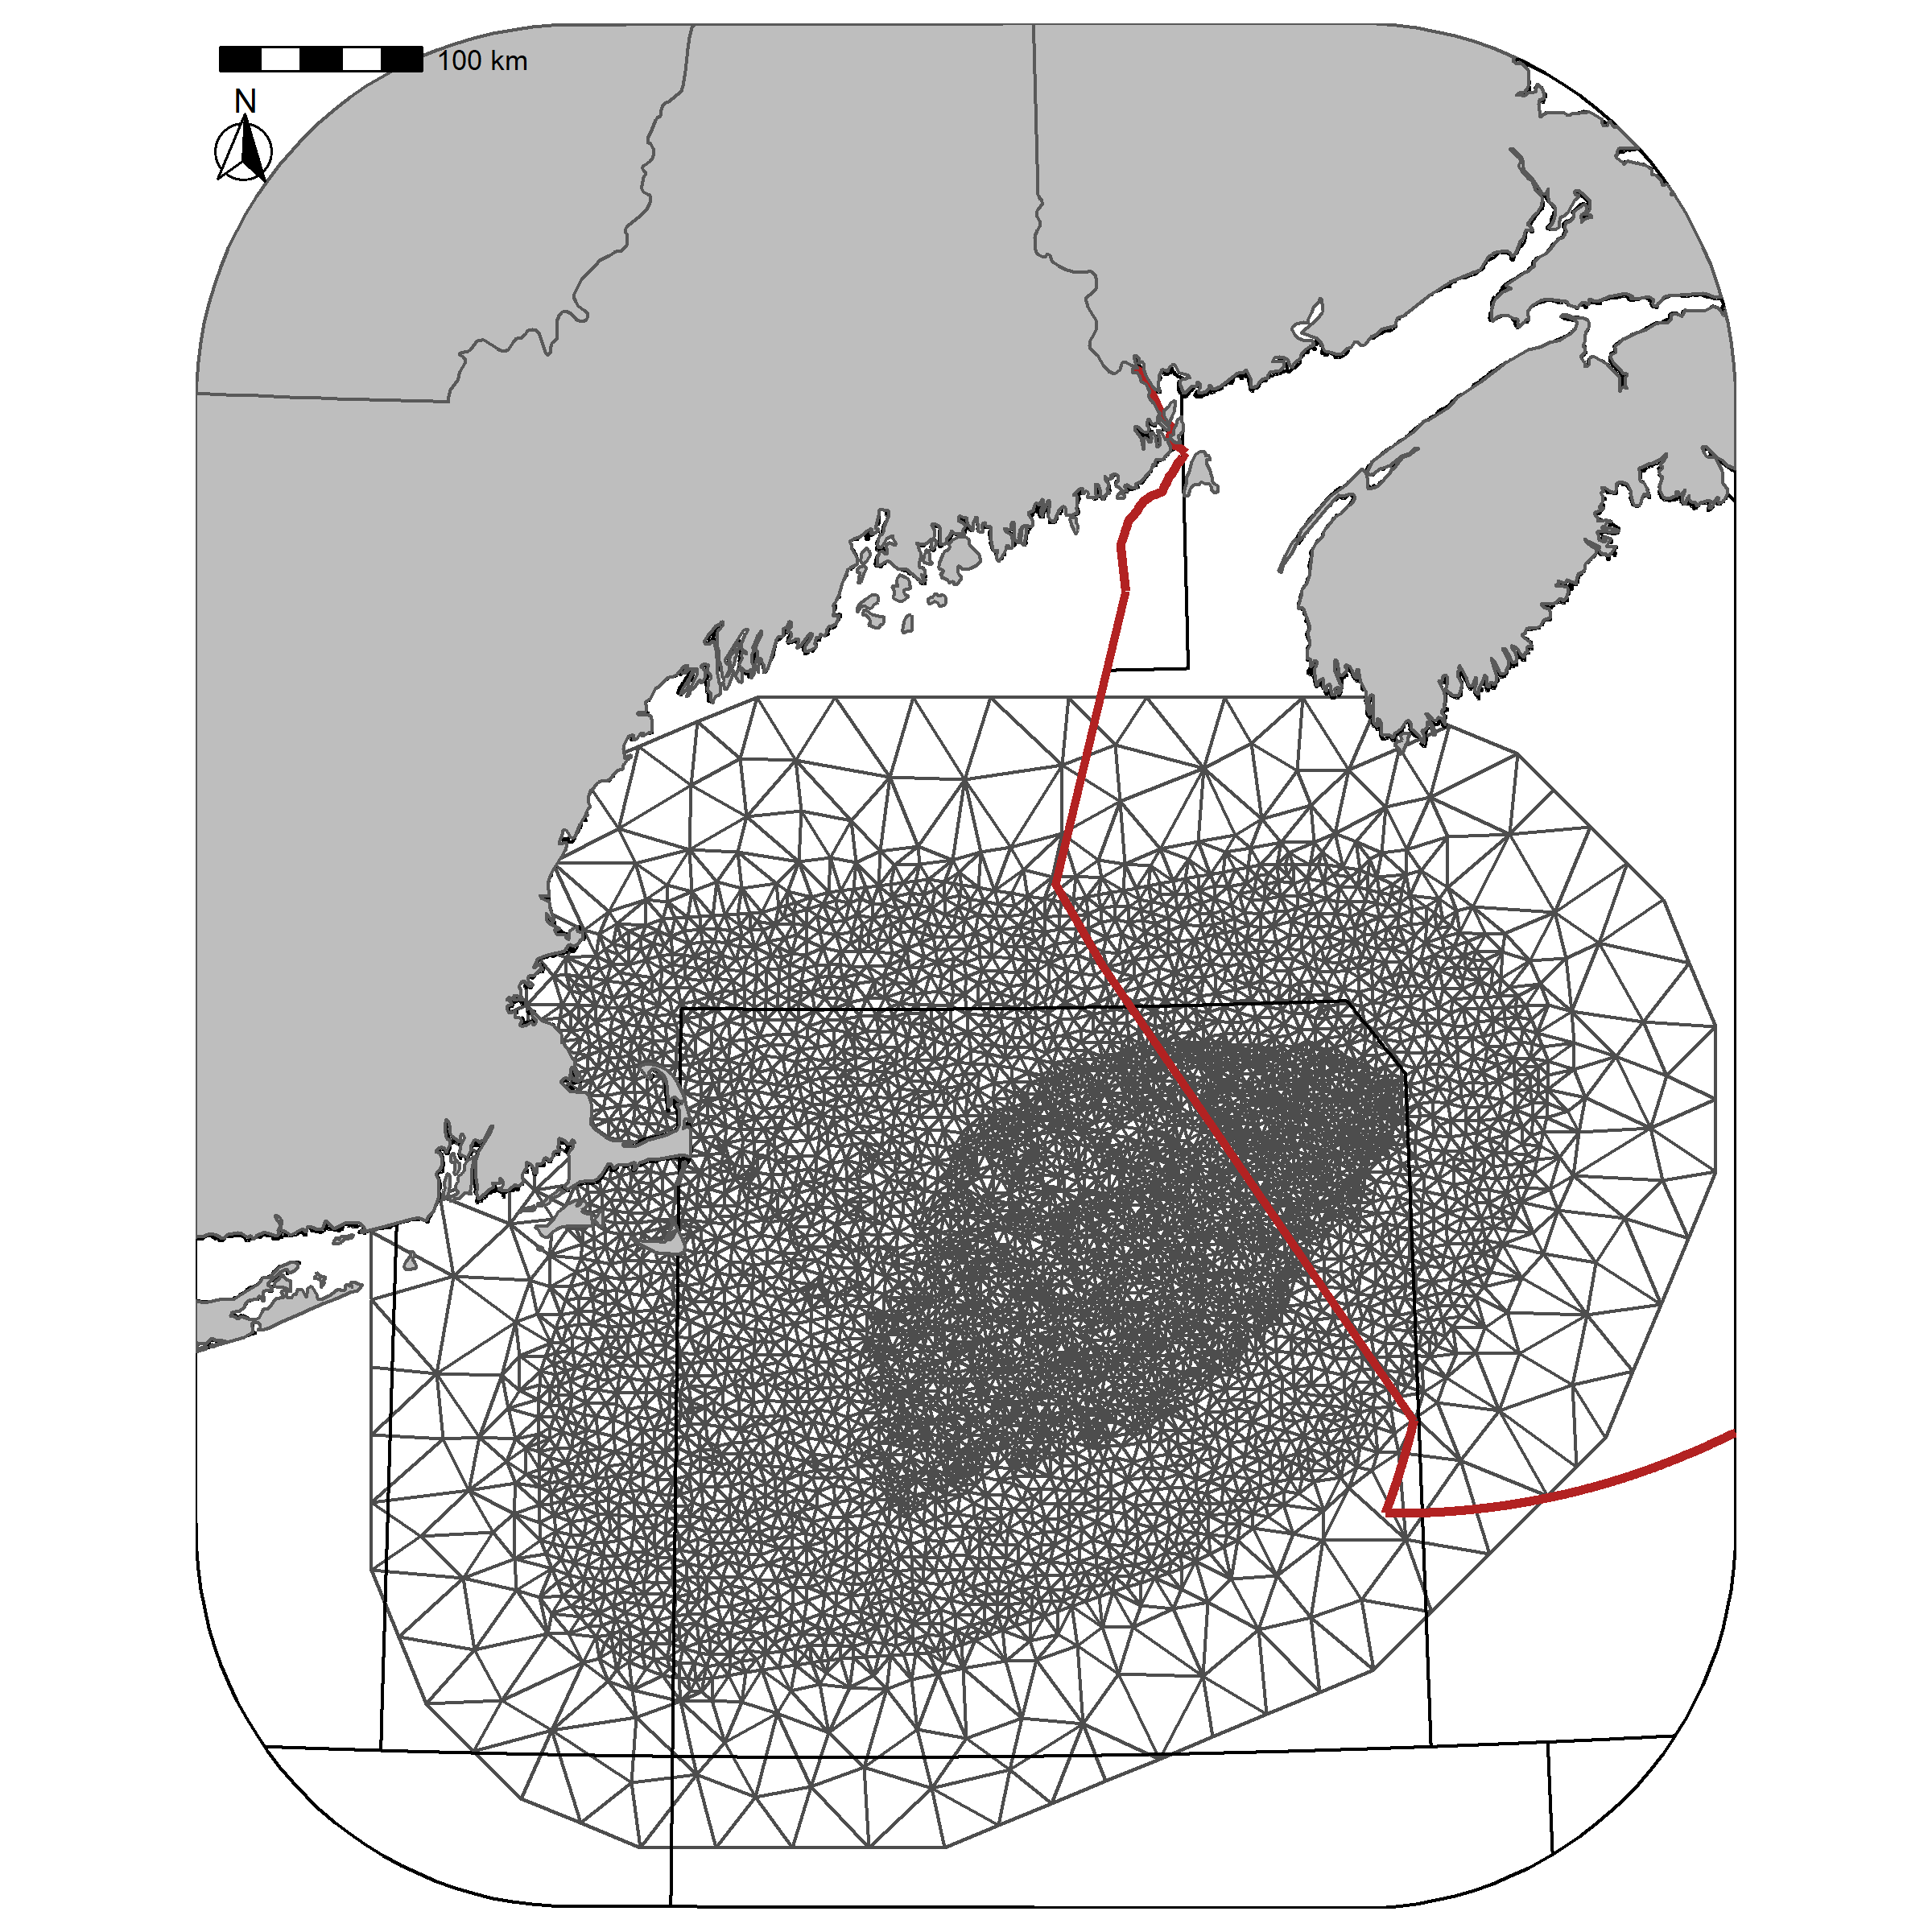
\includegraphics[width=1\linewidth]{D:/Github/Paper_2_SDMs/Results/Figures/mesh.grid} \caption{Prediction grid used for prediction of occurrence probability (OP).}\label{fig:mesh-grid}
\end{figure}

\clearpage
\begin{figure}
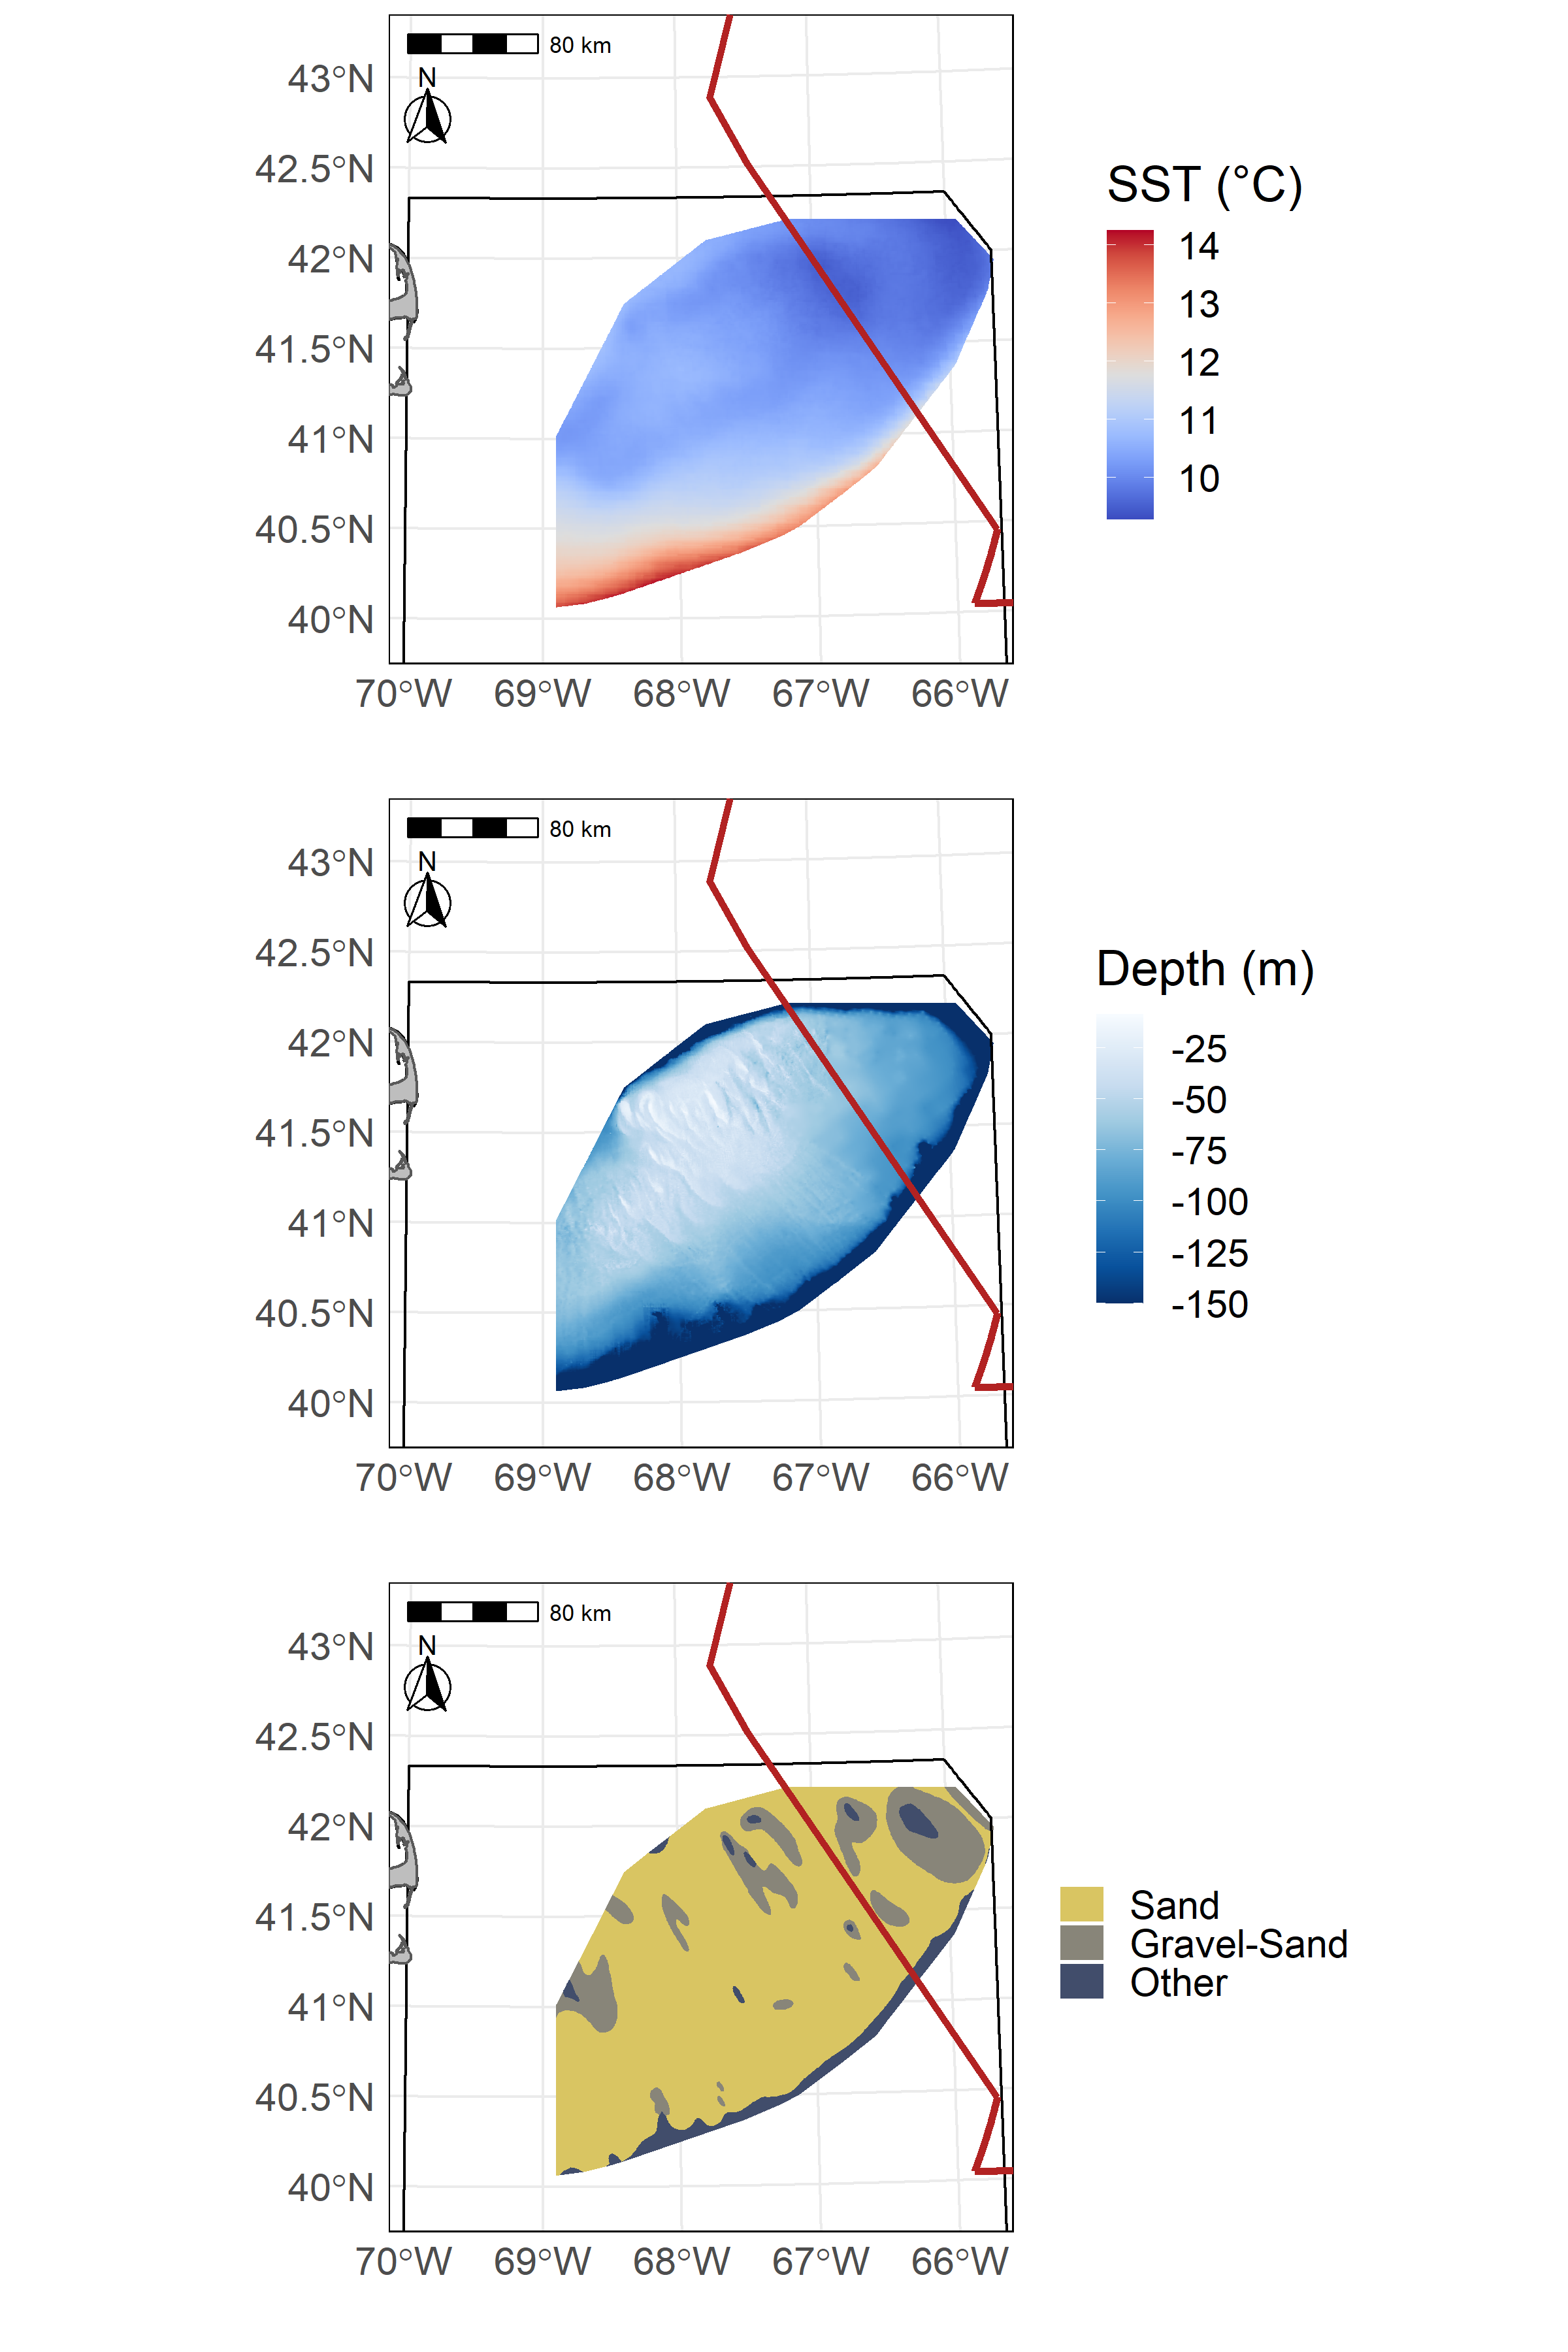
\includegraphics[width=1\linewidth]{D:/Github/Paper_2_SDMs/Results/Figures/depth_sst_sed_fields} \caption{Georges Bank (GB) Average Sea Surface Temperature from 1997-2008 (SST in °C) in the top panel, bathymetry (depth in meters) in the center panel, and sediment type in the bottom panel.}\label{fig:SST-Dep-Sed}
\end{figure}

\begin{landscape} 
\begin{figure}
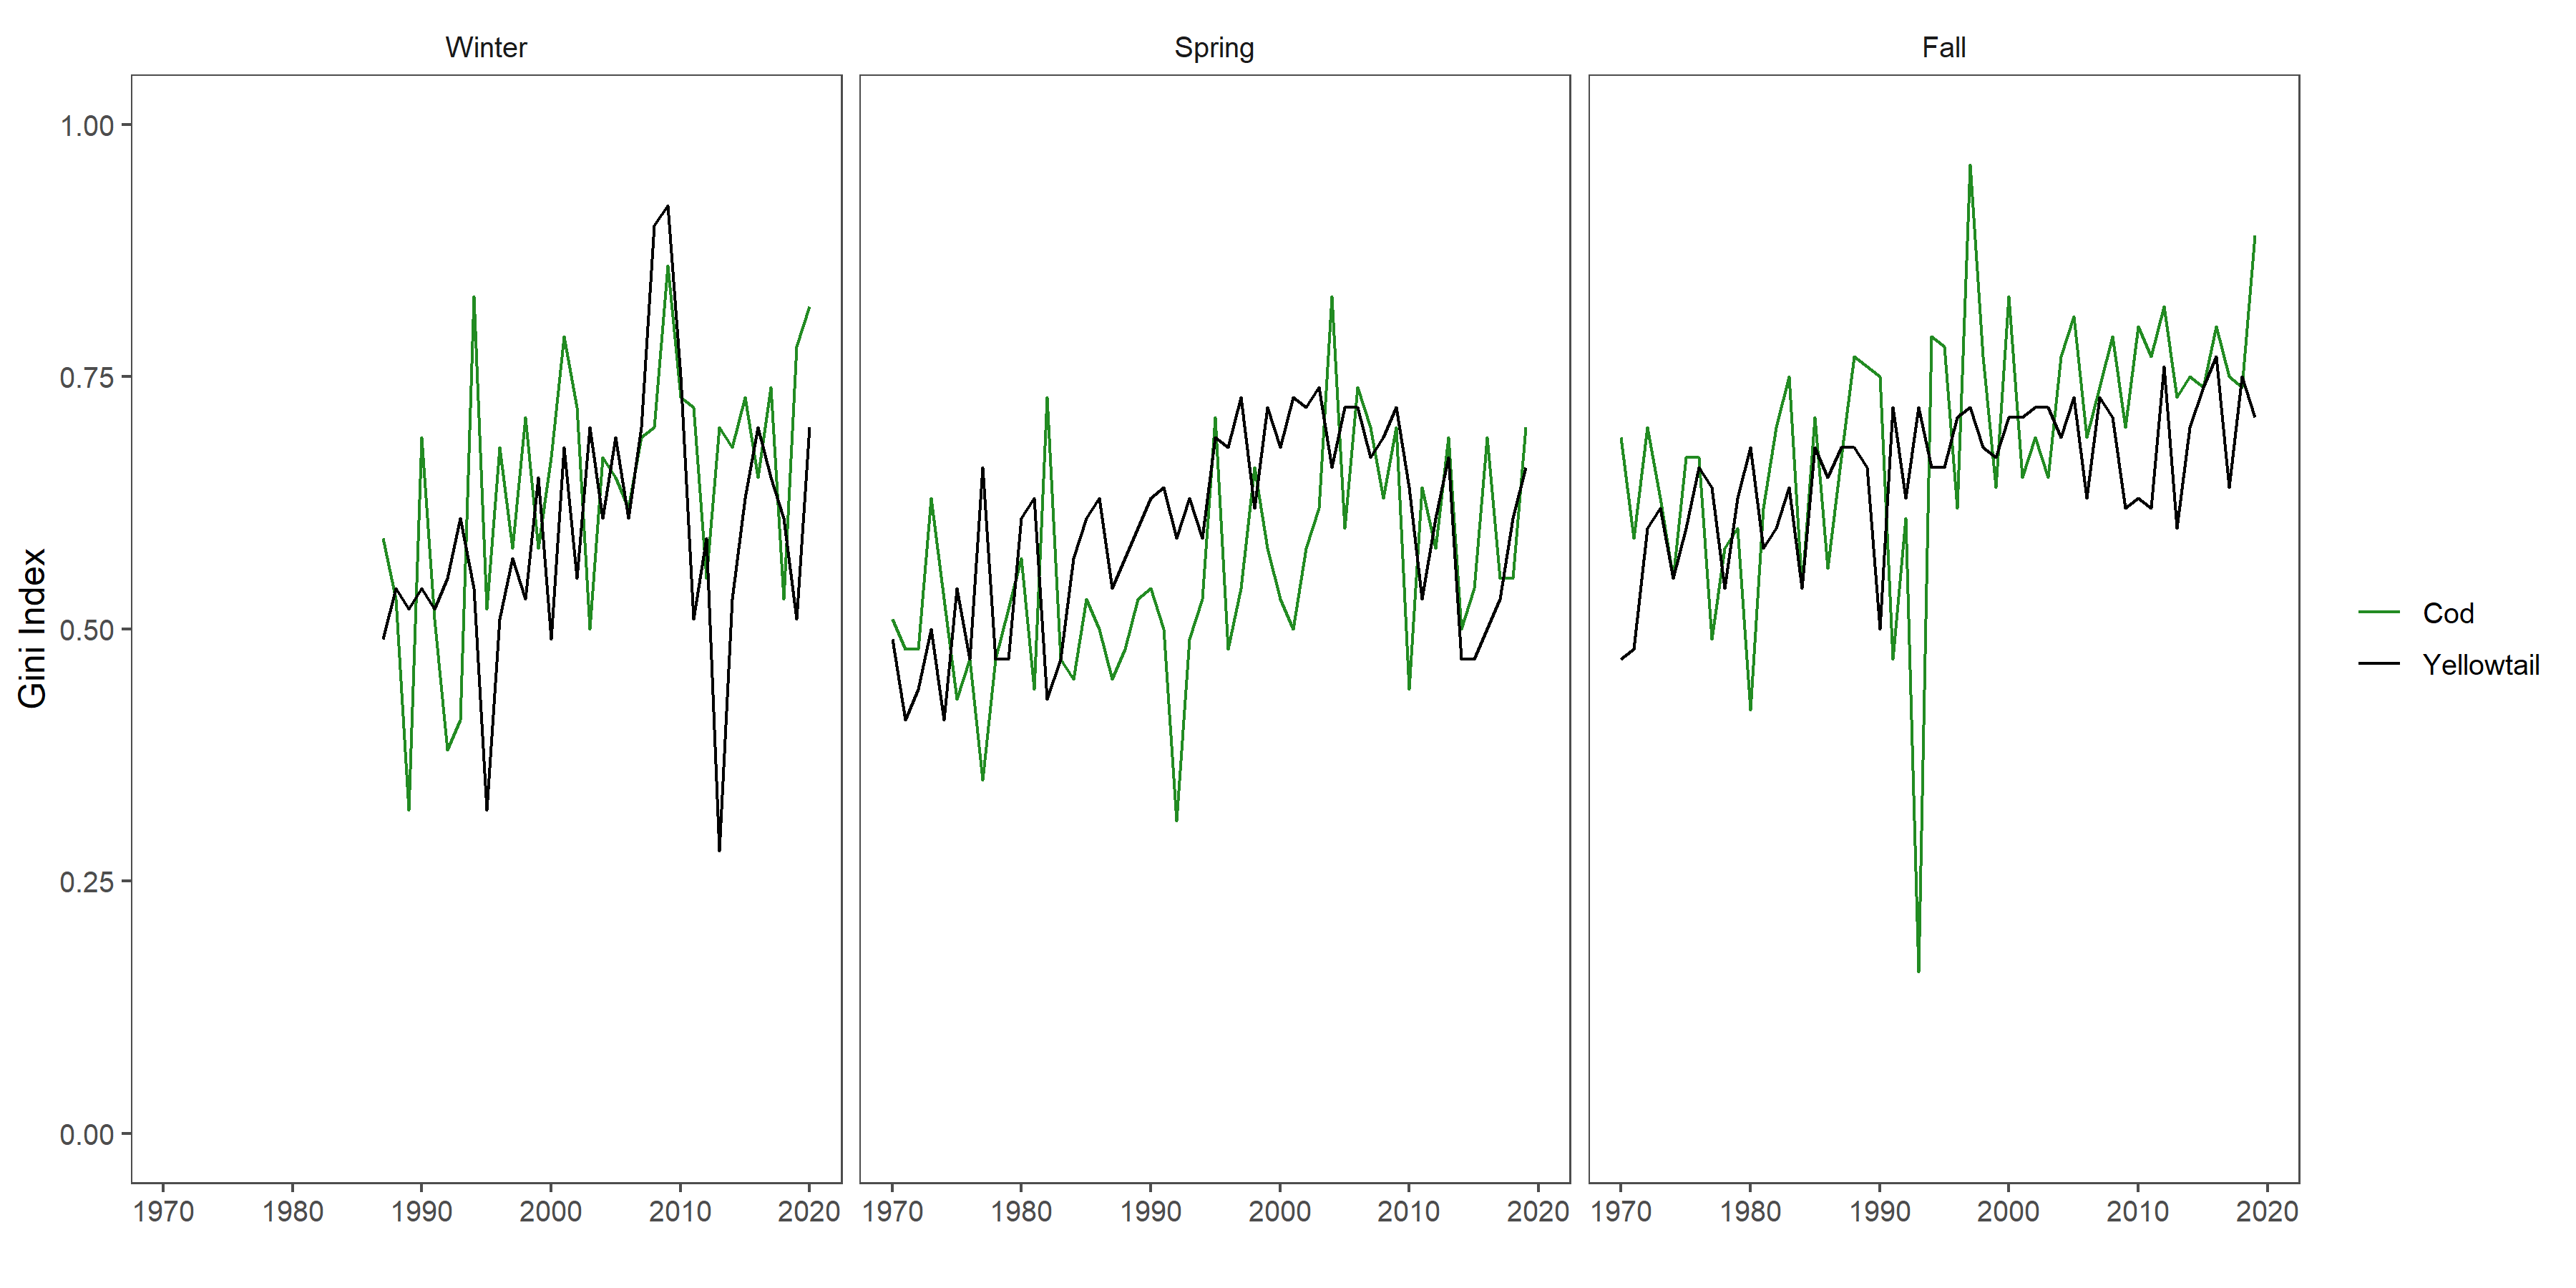
\includegraphics[width=1\linewidth]{D:/Github/Paper_2_SDMs/Results/Figures/Gini_index} \caption{Gini Index }\label{fig:gini-index}
\end{figure}
\end{landscape}

\hypertarget{model-selection}{%
\subsection{Model Selection}\label{model-selection}}

Stage 1 of model selection resulted in a significant reduction in the number of covariates. For Atlantic Cod, sea surface temperature (SST) was identified as a significant covariate in the \emph{Winter} and \emph{Spring}, in addition Dep and stratification were also significant predictors in the \emph{Spring}. In the \emph{Fall} no covariates had a WAIC that were a significant improvement from the intercept only model (Figure \ref{fig:diag-1-fe}). Further model selection indicated that an additive Dep + SST model was the \emph{final model} in all 3 seasons for Atlantic Cod (Figures \ref{fig:diag-2-fe} and \ref{fig:diag-3-fe}). When exploring the effect of temporal variability on the random fields, the models using the 5-year random field had the lowest WAIC in all seasons (Figure \ref{fig:diag-rf}).

For Yellowtail Flounder, stage 1 of model selection indicated that the inclusion of Dep significantly improved the models in all 3 seasons (surveys), while Sediment type (Sed) and chlorophyll concentration (Chl) in the \emph{Fall} had a similar impact on the model WAIC as Dep. As a result SST, Dep, Chl, and Sed were used to explore the development of more complex covariate models. For Yellowtail Flounder the best models in stage 2 of model selection included 2 covariates with a combination of Dep, SST, and Sed (Figure \ref{fig:diag-2-fe}). Further model selection indicated that the \emph{final model} for Yellowtail Flounder in all 3 seasons was an additive model including Dep, SST, and Sed (Figure \ref{fig:diag-3-fe}). When exploring the effect of temporal variability on the random fields, the 3-year field had the lowest WAIC in the \emph{Winter} and \emph{Spring}, while the 5-year field had the lowest WAIC in the \emph{Fall} (Figure \ref{fig:diag-rf}). Additional model selection results are available in the Model Output and Model Diagnostics sections of the interactive \href{https://github.com/Dave-Keith/Paper_2_SDMs/tree/master/Dashboard}{dashboard}.

\begin{landscape} 
\newpage
\begin{figure}
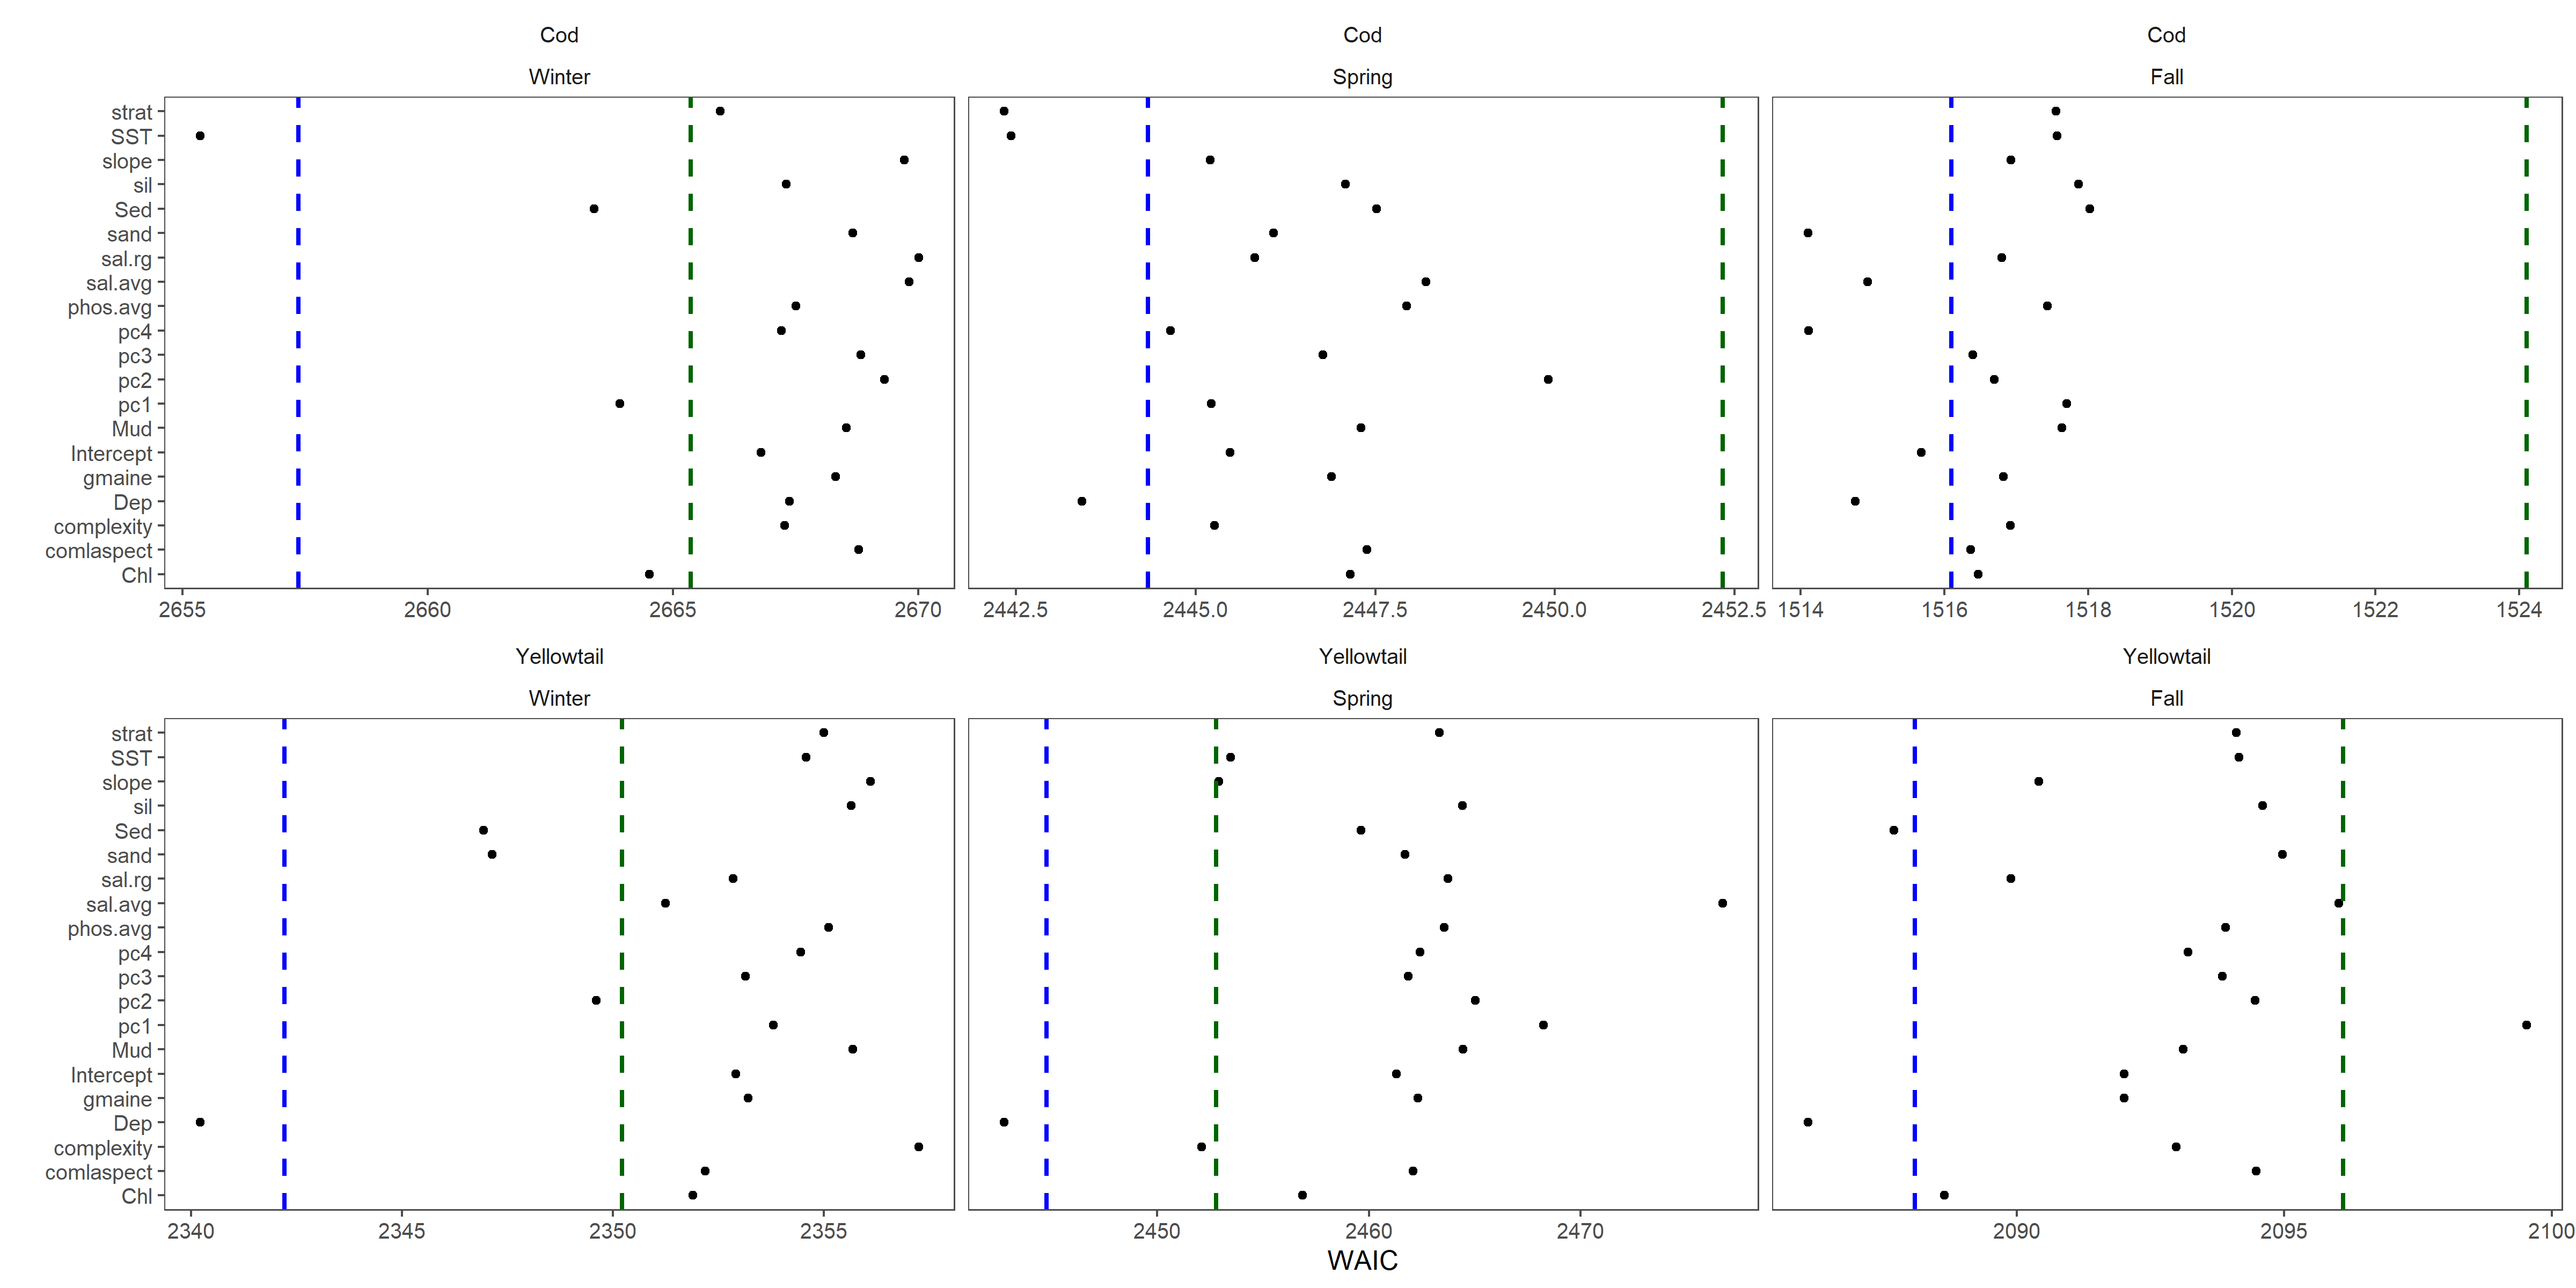
\includegraphics[width=1\linewidth]{D:/Github/Paper_2_SDMs/Results/Figures/Diagnostics_single_fe_waic} \caption{Initial stage of forward model selection using each of the environmental covariates individually.  This model selection was done using a static random field. Blue dashed line is 2 WAIC units larger than the model with the lowest WAIC, the green dashed line is 10 WAIC units larger than the model with the lowest WAIC. The full description of the environmental variables can be found in Table 1.}\label{fig:diag-1-fe}
\end{figure}

\newpage
\begin{figure}
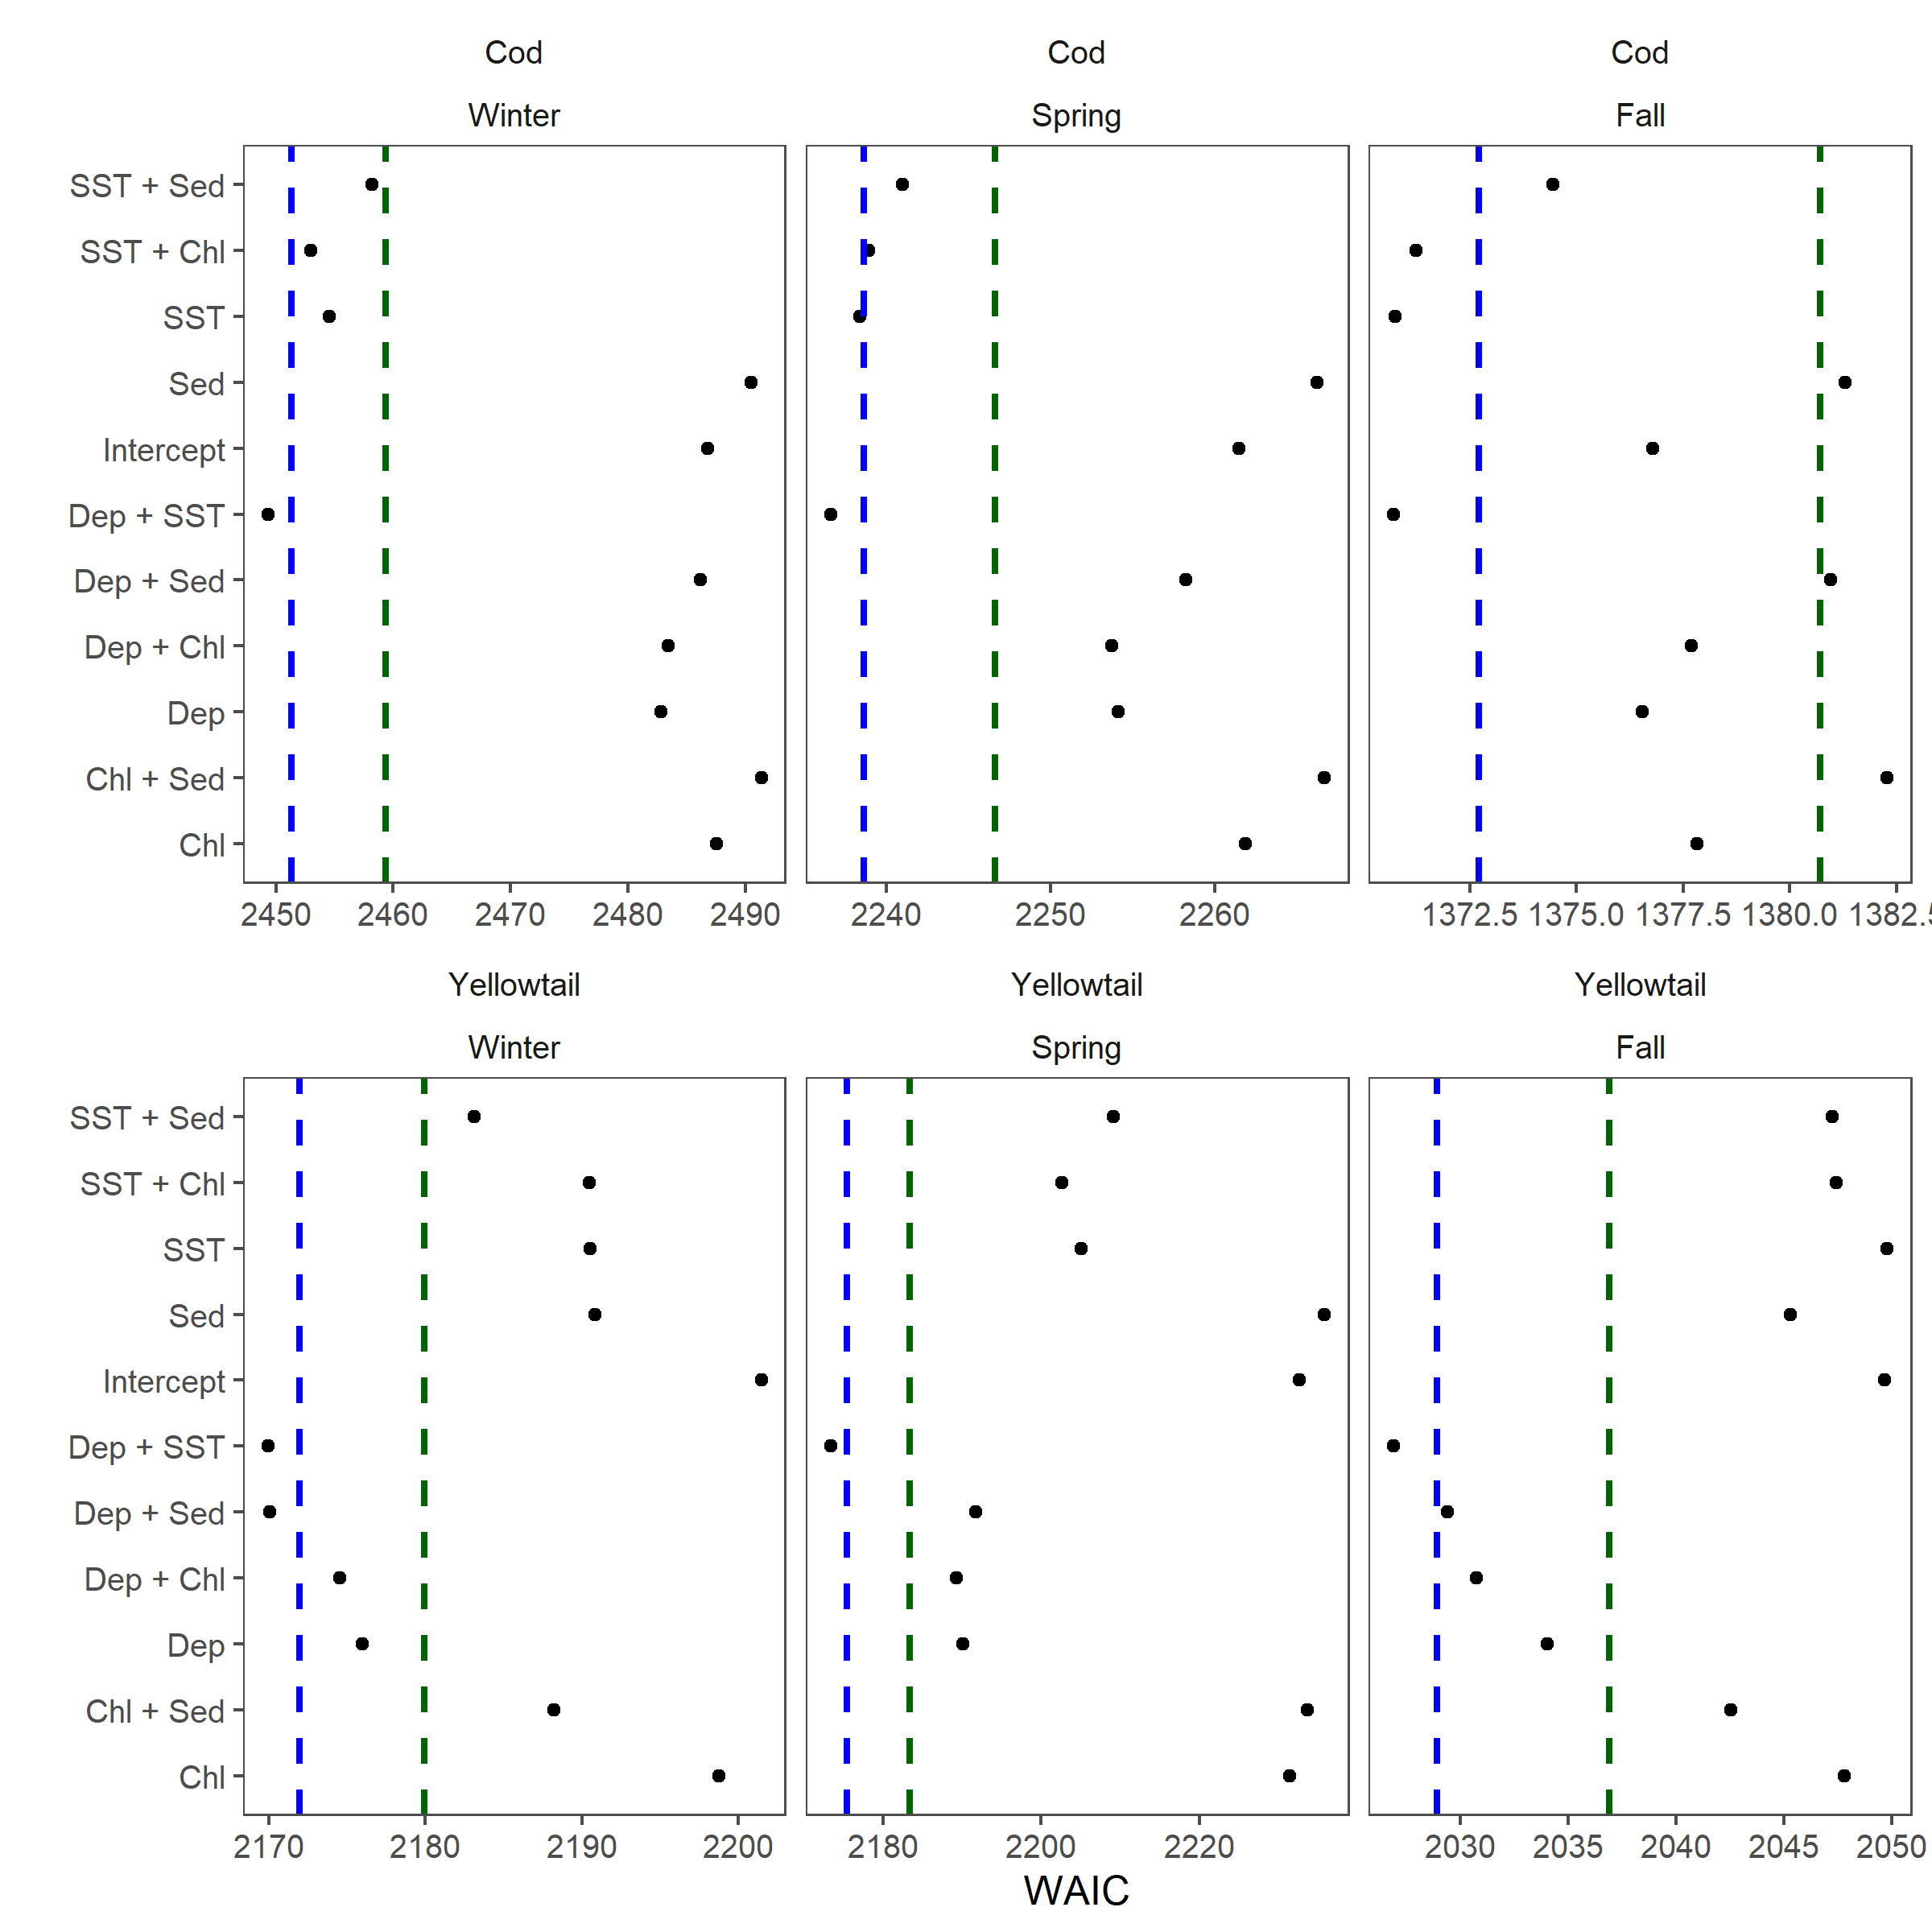
\includegraphics[width=1\linewidth]{D:/Github/Paper_2_SDMs/Results/Figures/Diagnostics_2_covars_fe_waic} \caption{Stage 2 of model selection including additive models with 2 covariates based on the covariates identified in the initial model selection stage. These models were compared using the 10-year random field models. Blue dashed line is 2 WAIC units larger than the model with the lowest WAIC, the green dashed line is 10 WAIC units larger than the model with the lowest WAIC. The full description of the environmental variables can be found in Table 1.}\label{fig:diag-2-fe}
\end{figure}

\newpage
\begin{figure}
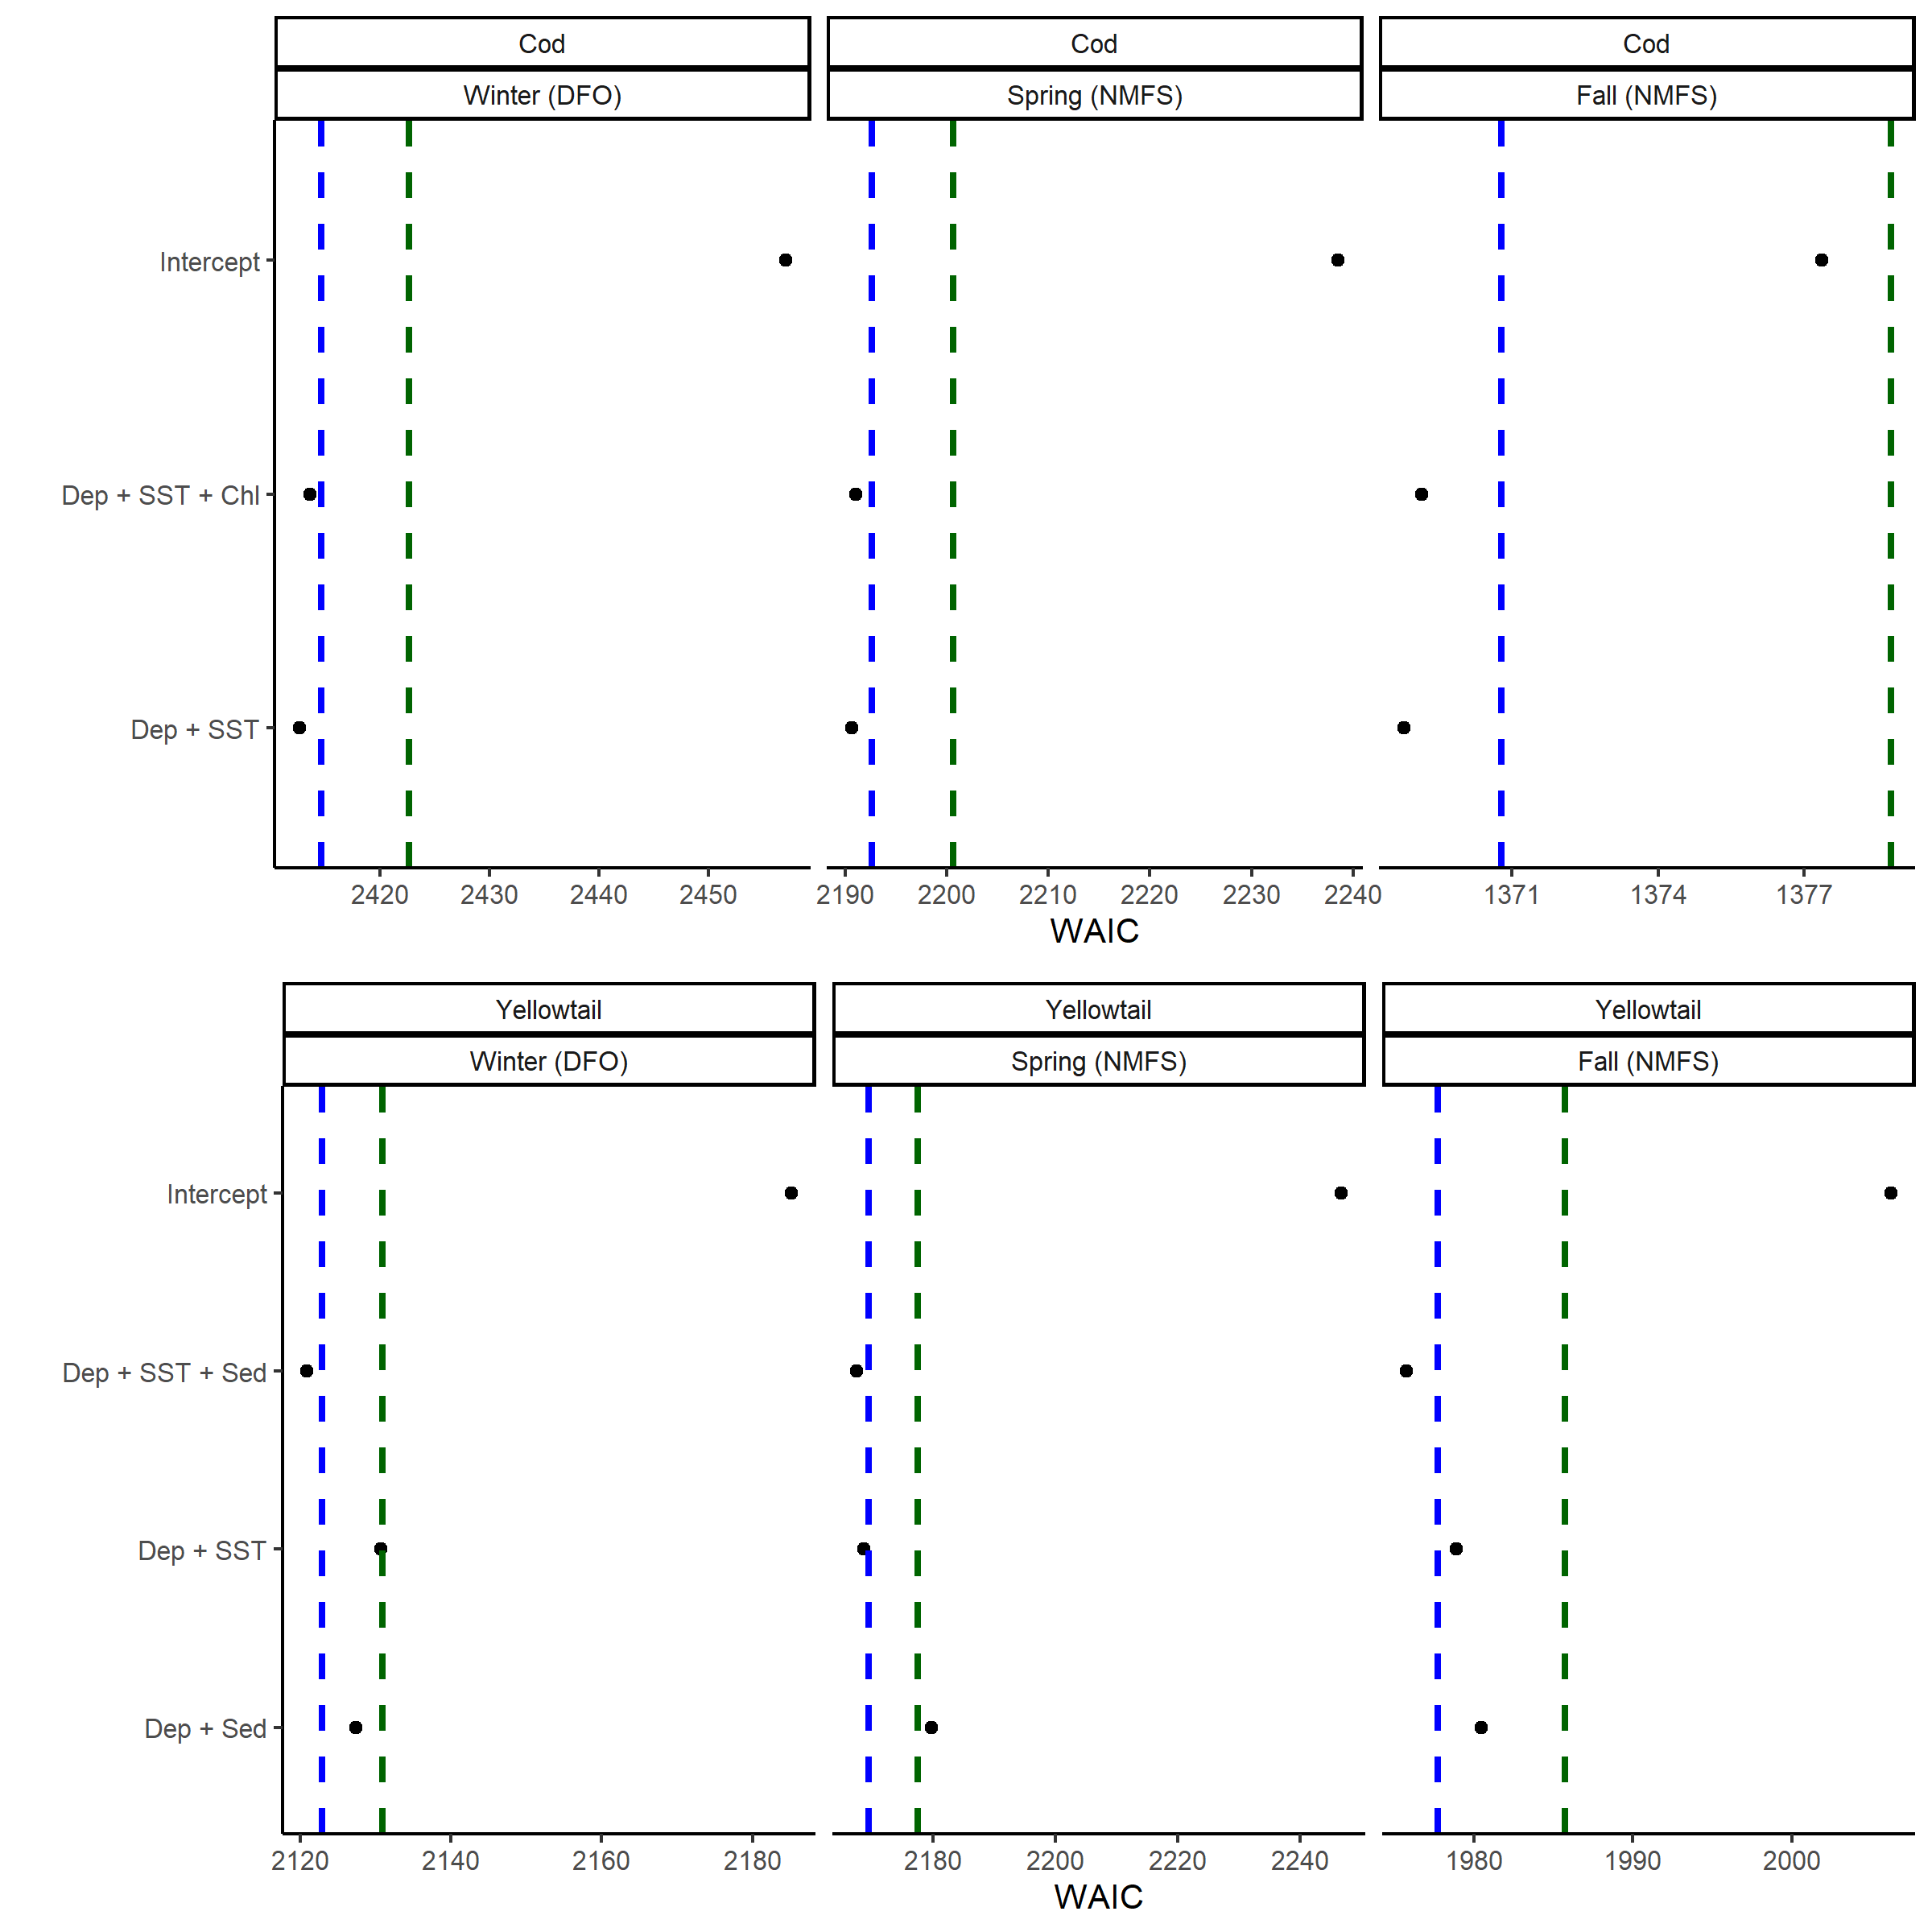
\includegraphics[width=1\linewidth]{D:/Github/Paper_2_SDMs/Results/Figures/Diagnostics_3_covars_fe_waic} \caption{Final stage of covariate model selection which includes model with up to 3 covariate terms based on models selected at stage 2. Blue dashed line is 2 WAIC units larger than the model with the lowest WAIC, the green dashed line is 10 WAIC units larger than the model with the lowest WAIC. The full description of the environmental variables can be found in Table 1.}\label{fig:diag-3-fe}
\end{figure}

\newpage
\begin{figure}
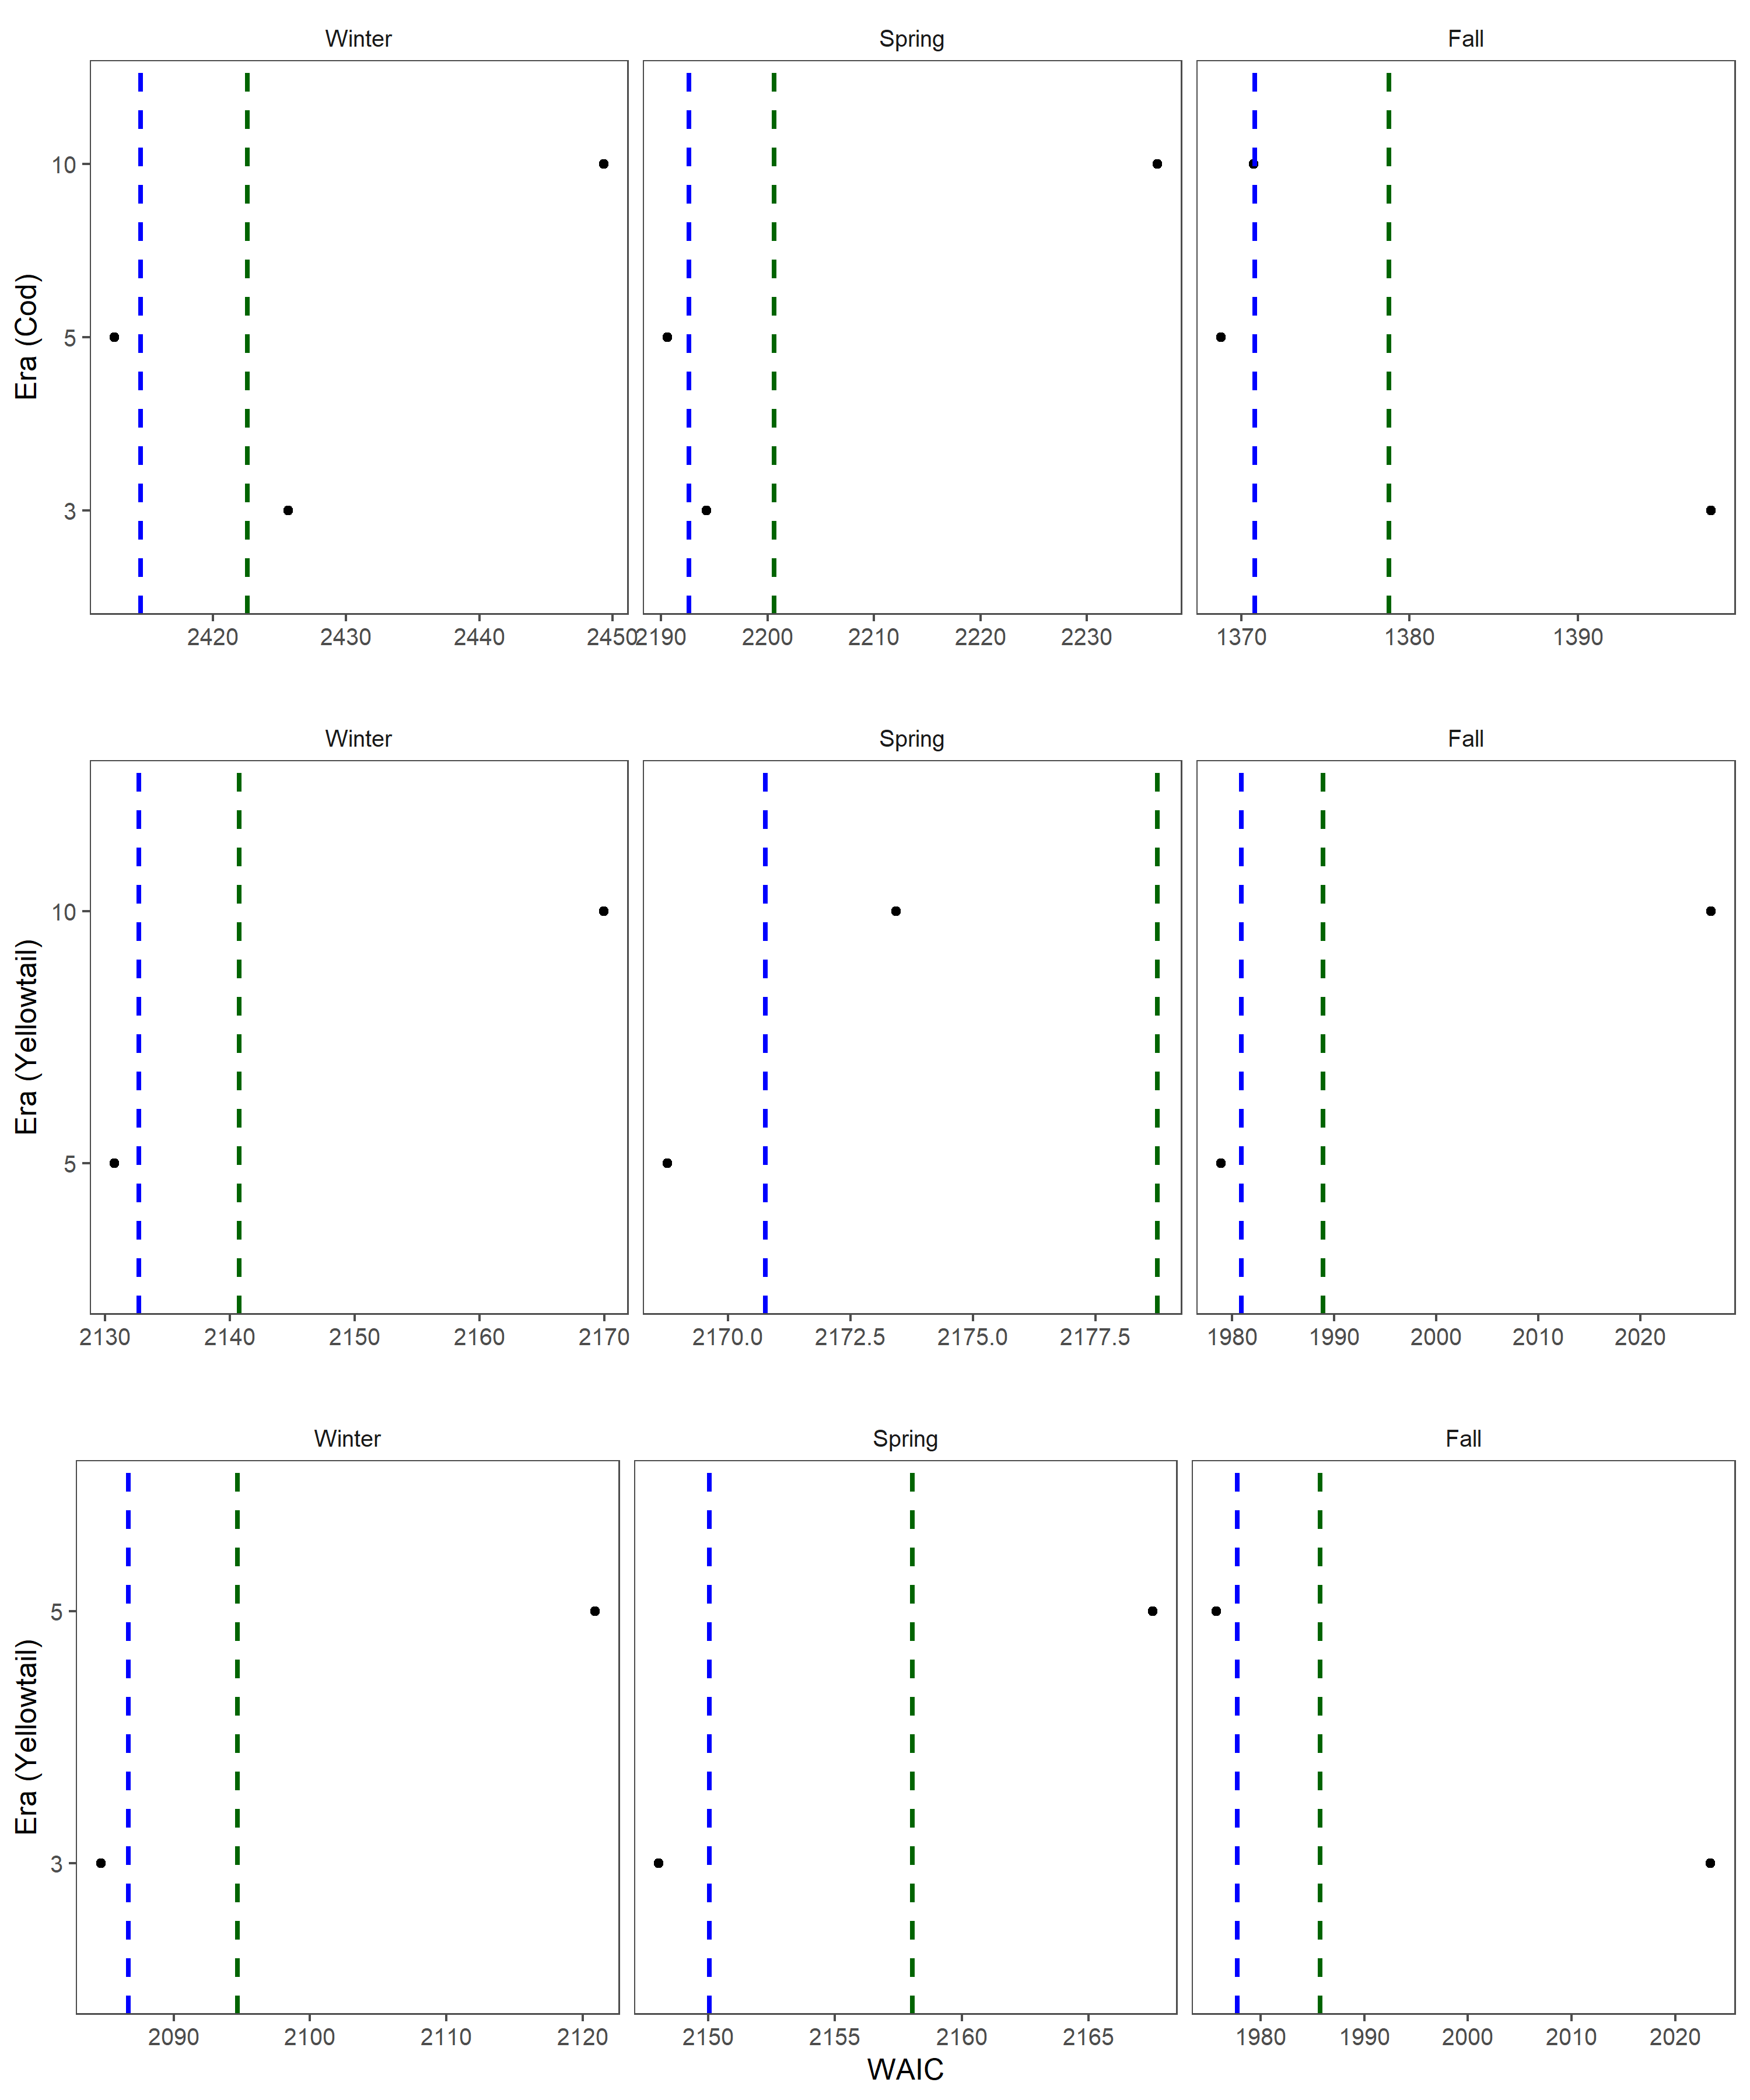
\includegraphics[width=1\linewidth]{D:/Github/Paper_2_SDMs/Results/Figures/Diagnostics_rf_waic} \caption{Model selection comparing the random fields models.  For cod the model used is Dep + SST for all of the random fields.  For Yellowtail the 5 and 10 year random fields were compared using the Dep + SST model, while the 5 and 3 fields were compared using the slightly preferred Dep + SST + Sed model. Blue dashed line is 2 WAIC units larger than the model with the lowest WAIC, the green dashed line is 10 WAIC units larger than the model with the lowest WAIC.}\label{fig:diag-rf}
\end{figure}
\end{landscape}

\clearpage

\hypertarget{predicted-occurrence-probability}{%
\section{Predicted Occurrence Probability}\label{predicted-occurrence-probability}}

The modeled OP for Atlantic Cod in the \emph{Winter} and \emph{Spring} was elevated on all but the most southern portion of GB in the 1970s and 1980s, in the early 1990s there was an abrupt decline in the OP throughout much of the U.S. portion of GB, while OP remained elevated in Canadian waters and in the area straddling the ICJ line (Figures \ref{fig:pf-winter-cod} - \ref{fig:pf-spring-cod}). In the \emph{Fall} the core areas were isolated in northern of GB. An area on the northwest of GB had some core area until the early 1980s but the OP in this area declined steadily after this time and has had a low OP in the \emph{Fall} for over 20 years, the highest OP areas remaining during the \emph{Fall} are along the northern edge of the bank and mostly in Canadian waters (Figure \ref{fig:pf-fall-cod}).

The modeled OP patterns for Yellowtail Flounder on GB are similar in the \emph{Winter}, \emph{Spring}, and \emph{Fall} with core area consistently observed in the region straddling the ICJ line in each season and throughout the study period (Figures \ref{fig:pf-winter-yt} - \ref{fig:pf-fall-yt}). A second region along the western border of the bank also has an elevated OP and appears to be connected via a narrow band of varying width to the core area straddling the ICJ line. The core area of Yellowtail Flounder declined in the late 1980s and early 1990s and was relatively stable until 2016 (Figure \ref{fig:pf-fall-yt}).

The standard deviation (SD) of the Atlantic Cod prediction field in the \emph{Winter} and \emph{Spring} tended to be elevated in the central portion of the bank, and lowest in the south and along the edges of the prediction domain. In the \emph{Fall} the Atlantic Cod prediction field SD was lowest in the south, with the low SD area expanding to central regions later in the study period (Figures \ref{fig:pf-winter-cod-sd} - \ref{fig:pf-fall-cod-sd}). For Yellowtail Flounder, the SD was consistently low in the part of the region with a core area that straddled the ICJ line in the \emph{Winter}, \emph{Spring}, and \emph{Fall} (Figures \ref{fig:pf-winter-yt-sd} - \ref{fig:pf-fall-yt-sd}). Areas surrounding this region displayed an increase in the SD, while a region in the north and along the southern flank of GB had relatively low SDs; these regions also had relatively low OPs (Figures \ref{fig:pf-winter-yt} - \ref{fig:pf-fall-yt} and \ref{fig:pf-winter-yt-sd} - \ref{fig:pf-fall-yt-sd}).

\newpage
\begin{landscape}
\begin{figure}
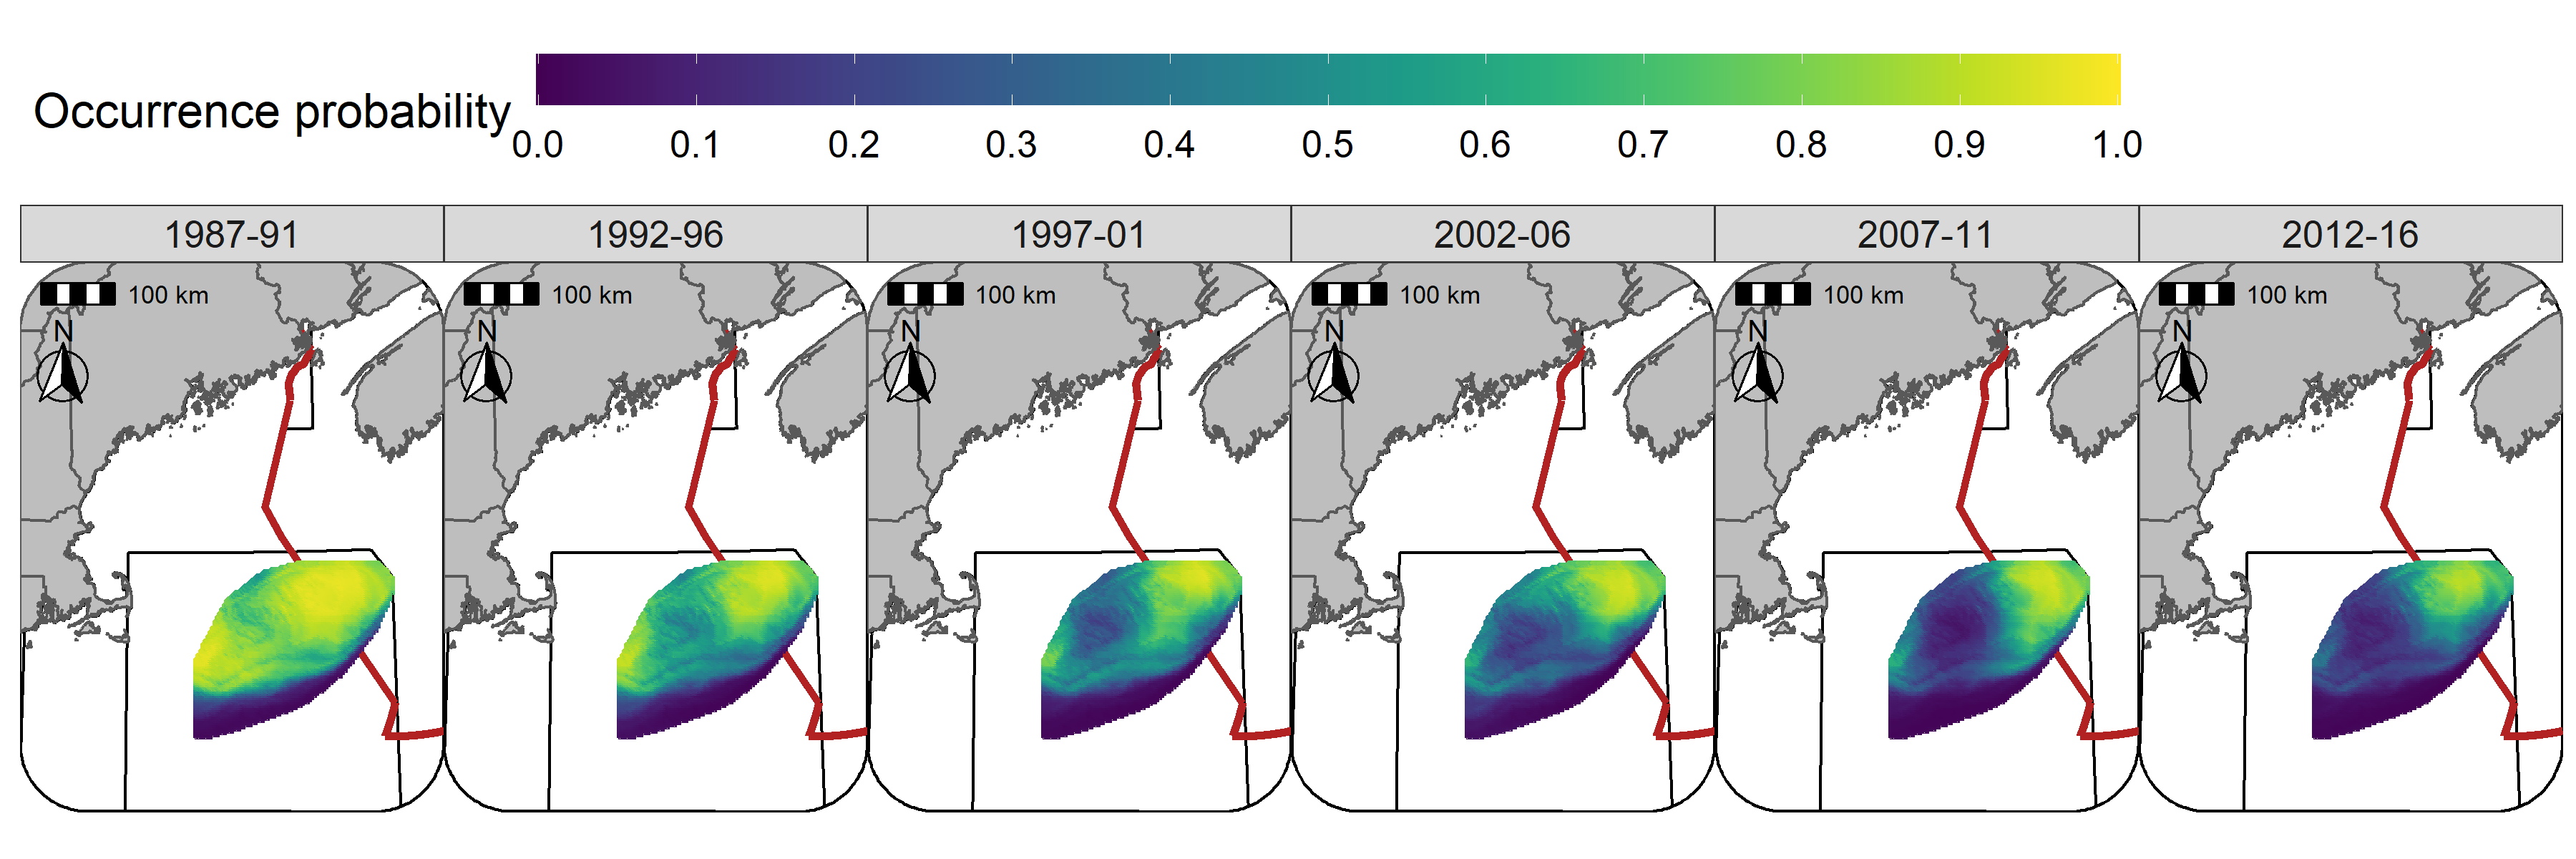
\includegraphics[width=1\linewidth]{D:/Github/Paper_2_SDMs/Results/Figures/pf_winter_cod} \caption{Predicted occurrence probability for Atlantic Cod  in each era during the Winter (RV survey) using the SST + Dep model and 5-year random field.}\label{fig:pf-winter-cod}
\end{figure}

\newpage
\begin{figure}
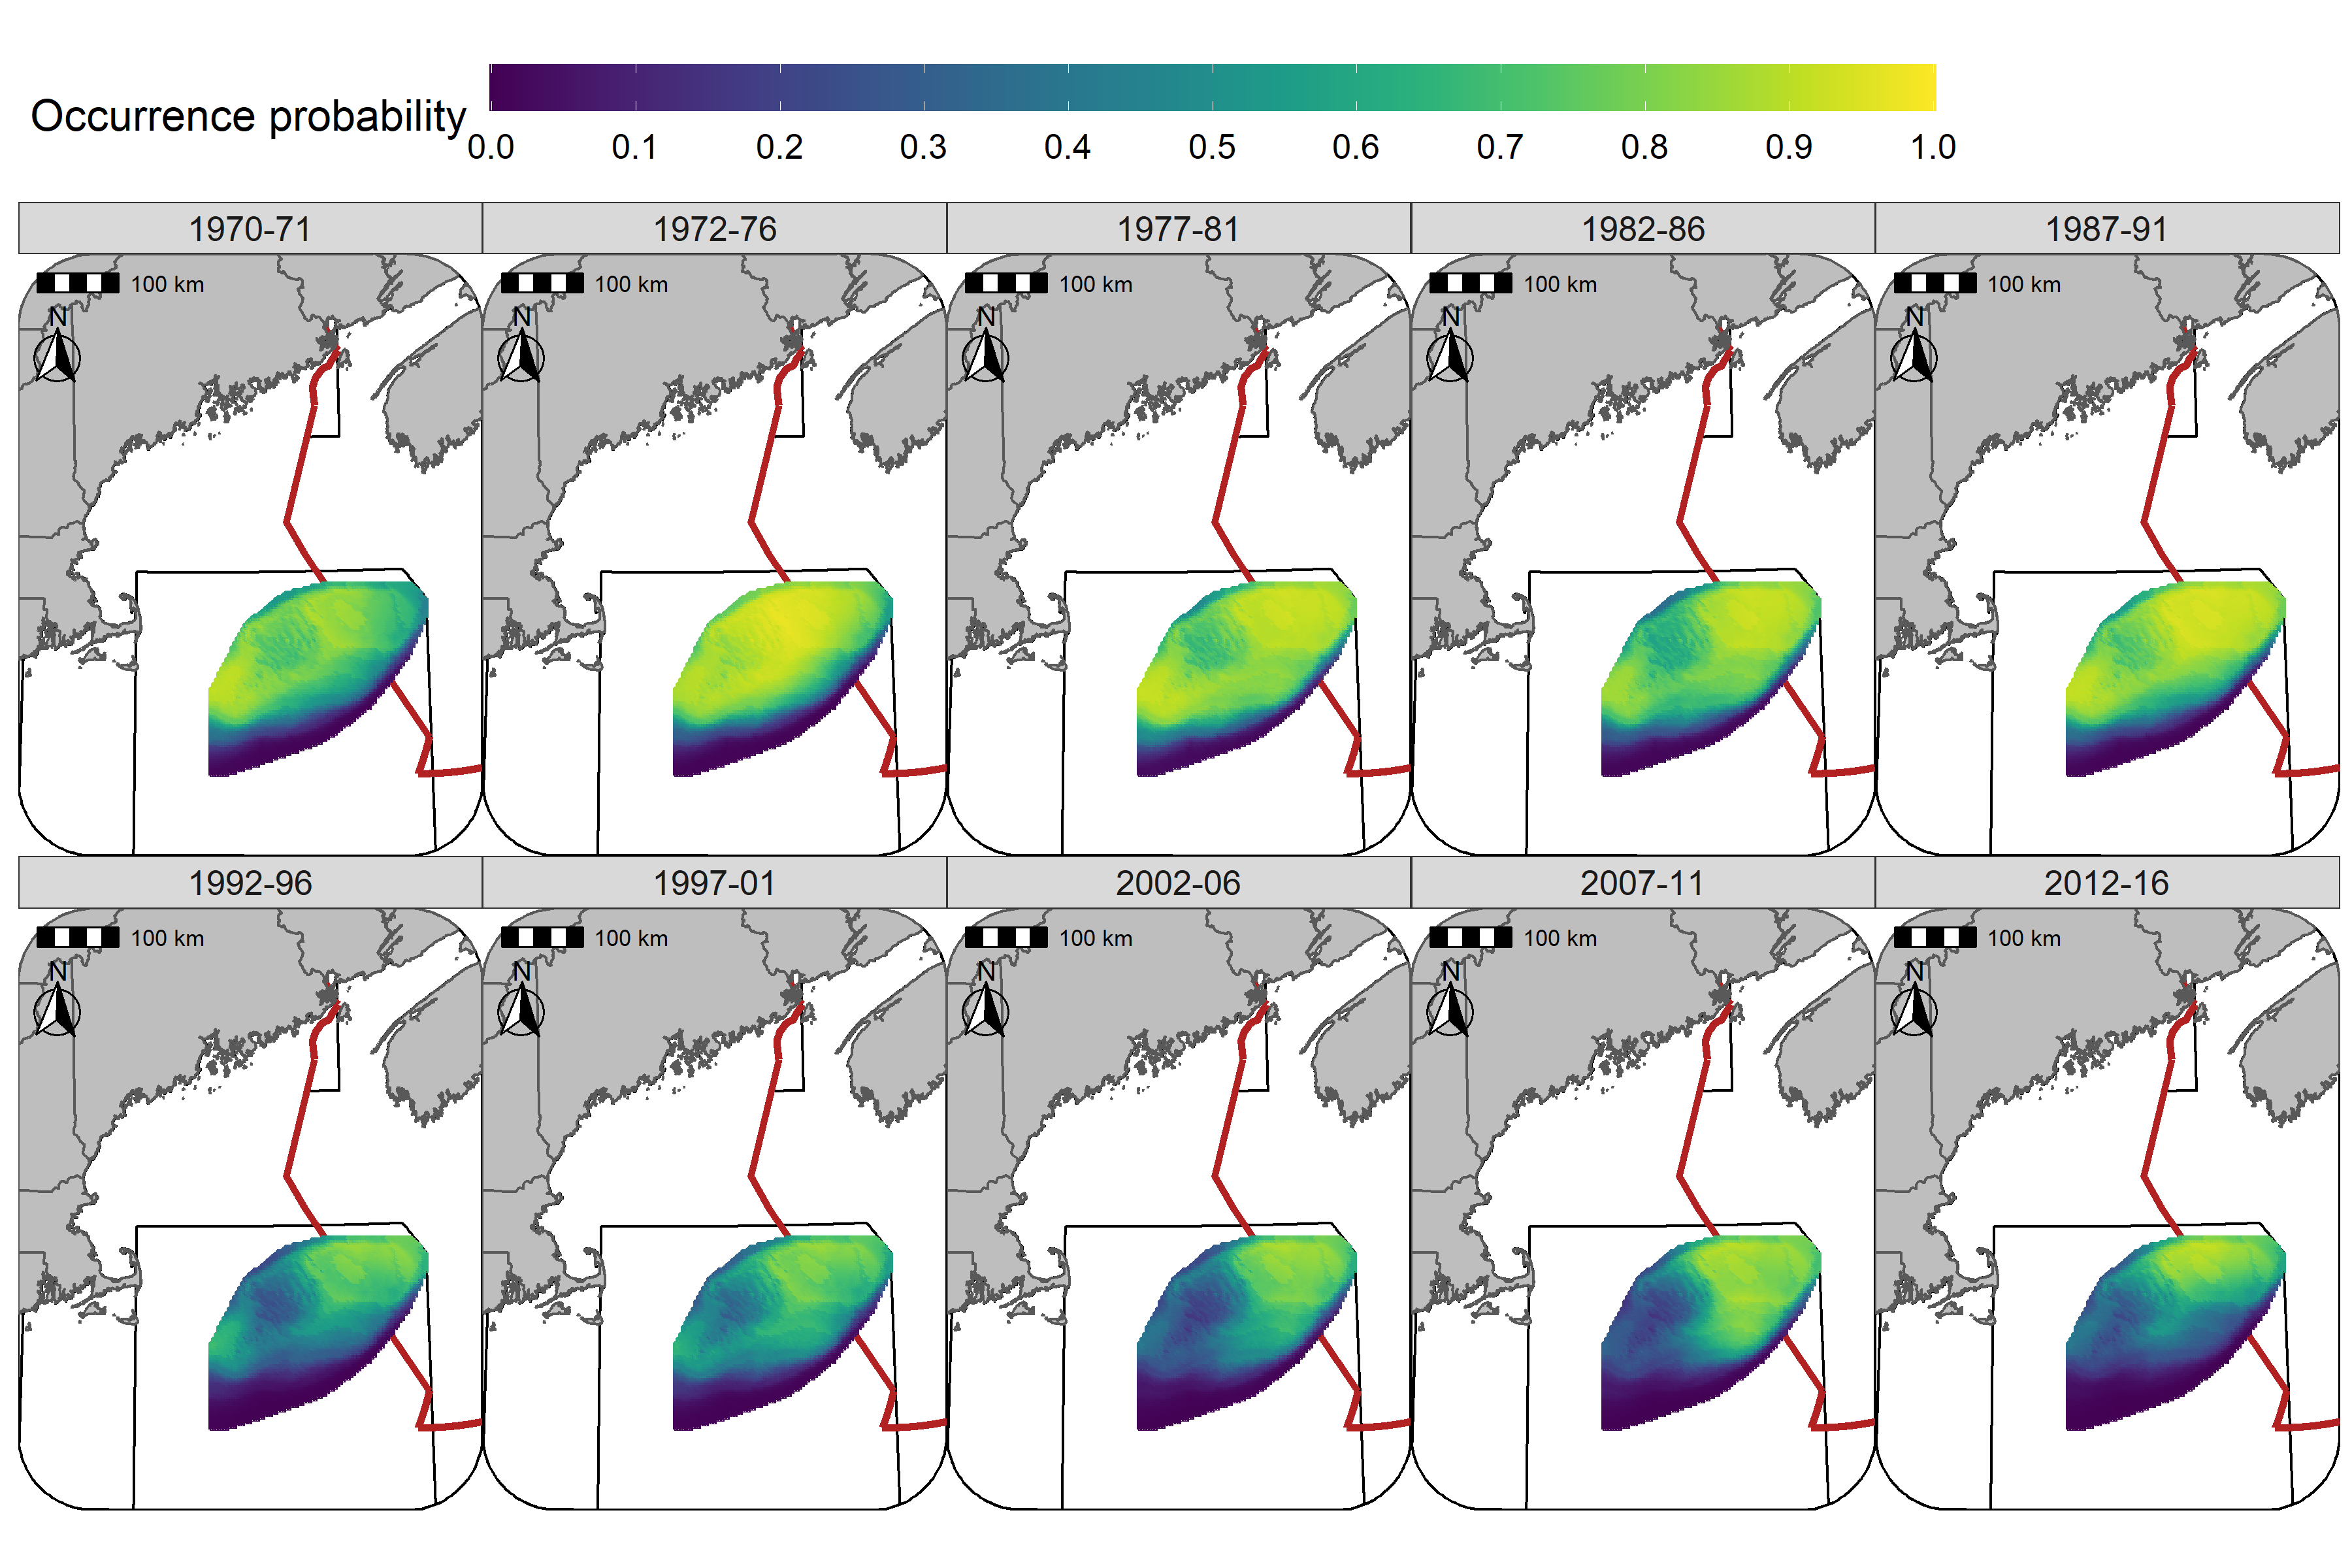
\includegraphics[width=1\linewidth]{D:/Github/Paper_2_SDMs/Results/Figures/pf_spring_cod} \caption{Predicted occurrence probability for Atlantic Cod  in each era during the Spring (NMFS-spring survey) using the SST + Dep model and 5-year random field.}\label{fig:pf-spring-cod}
\end{figure}

\newpage
\begin{figure}
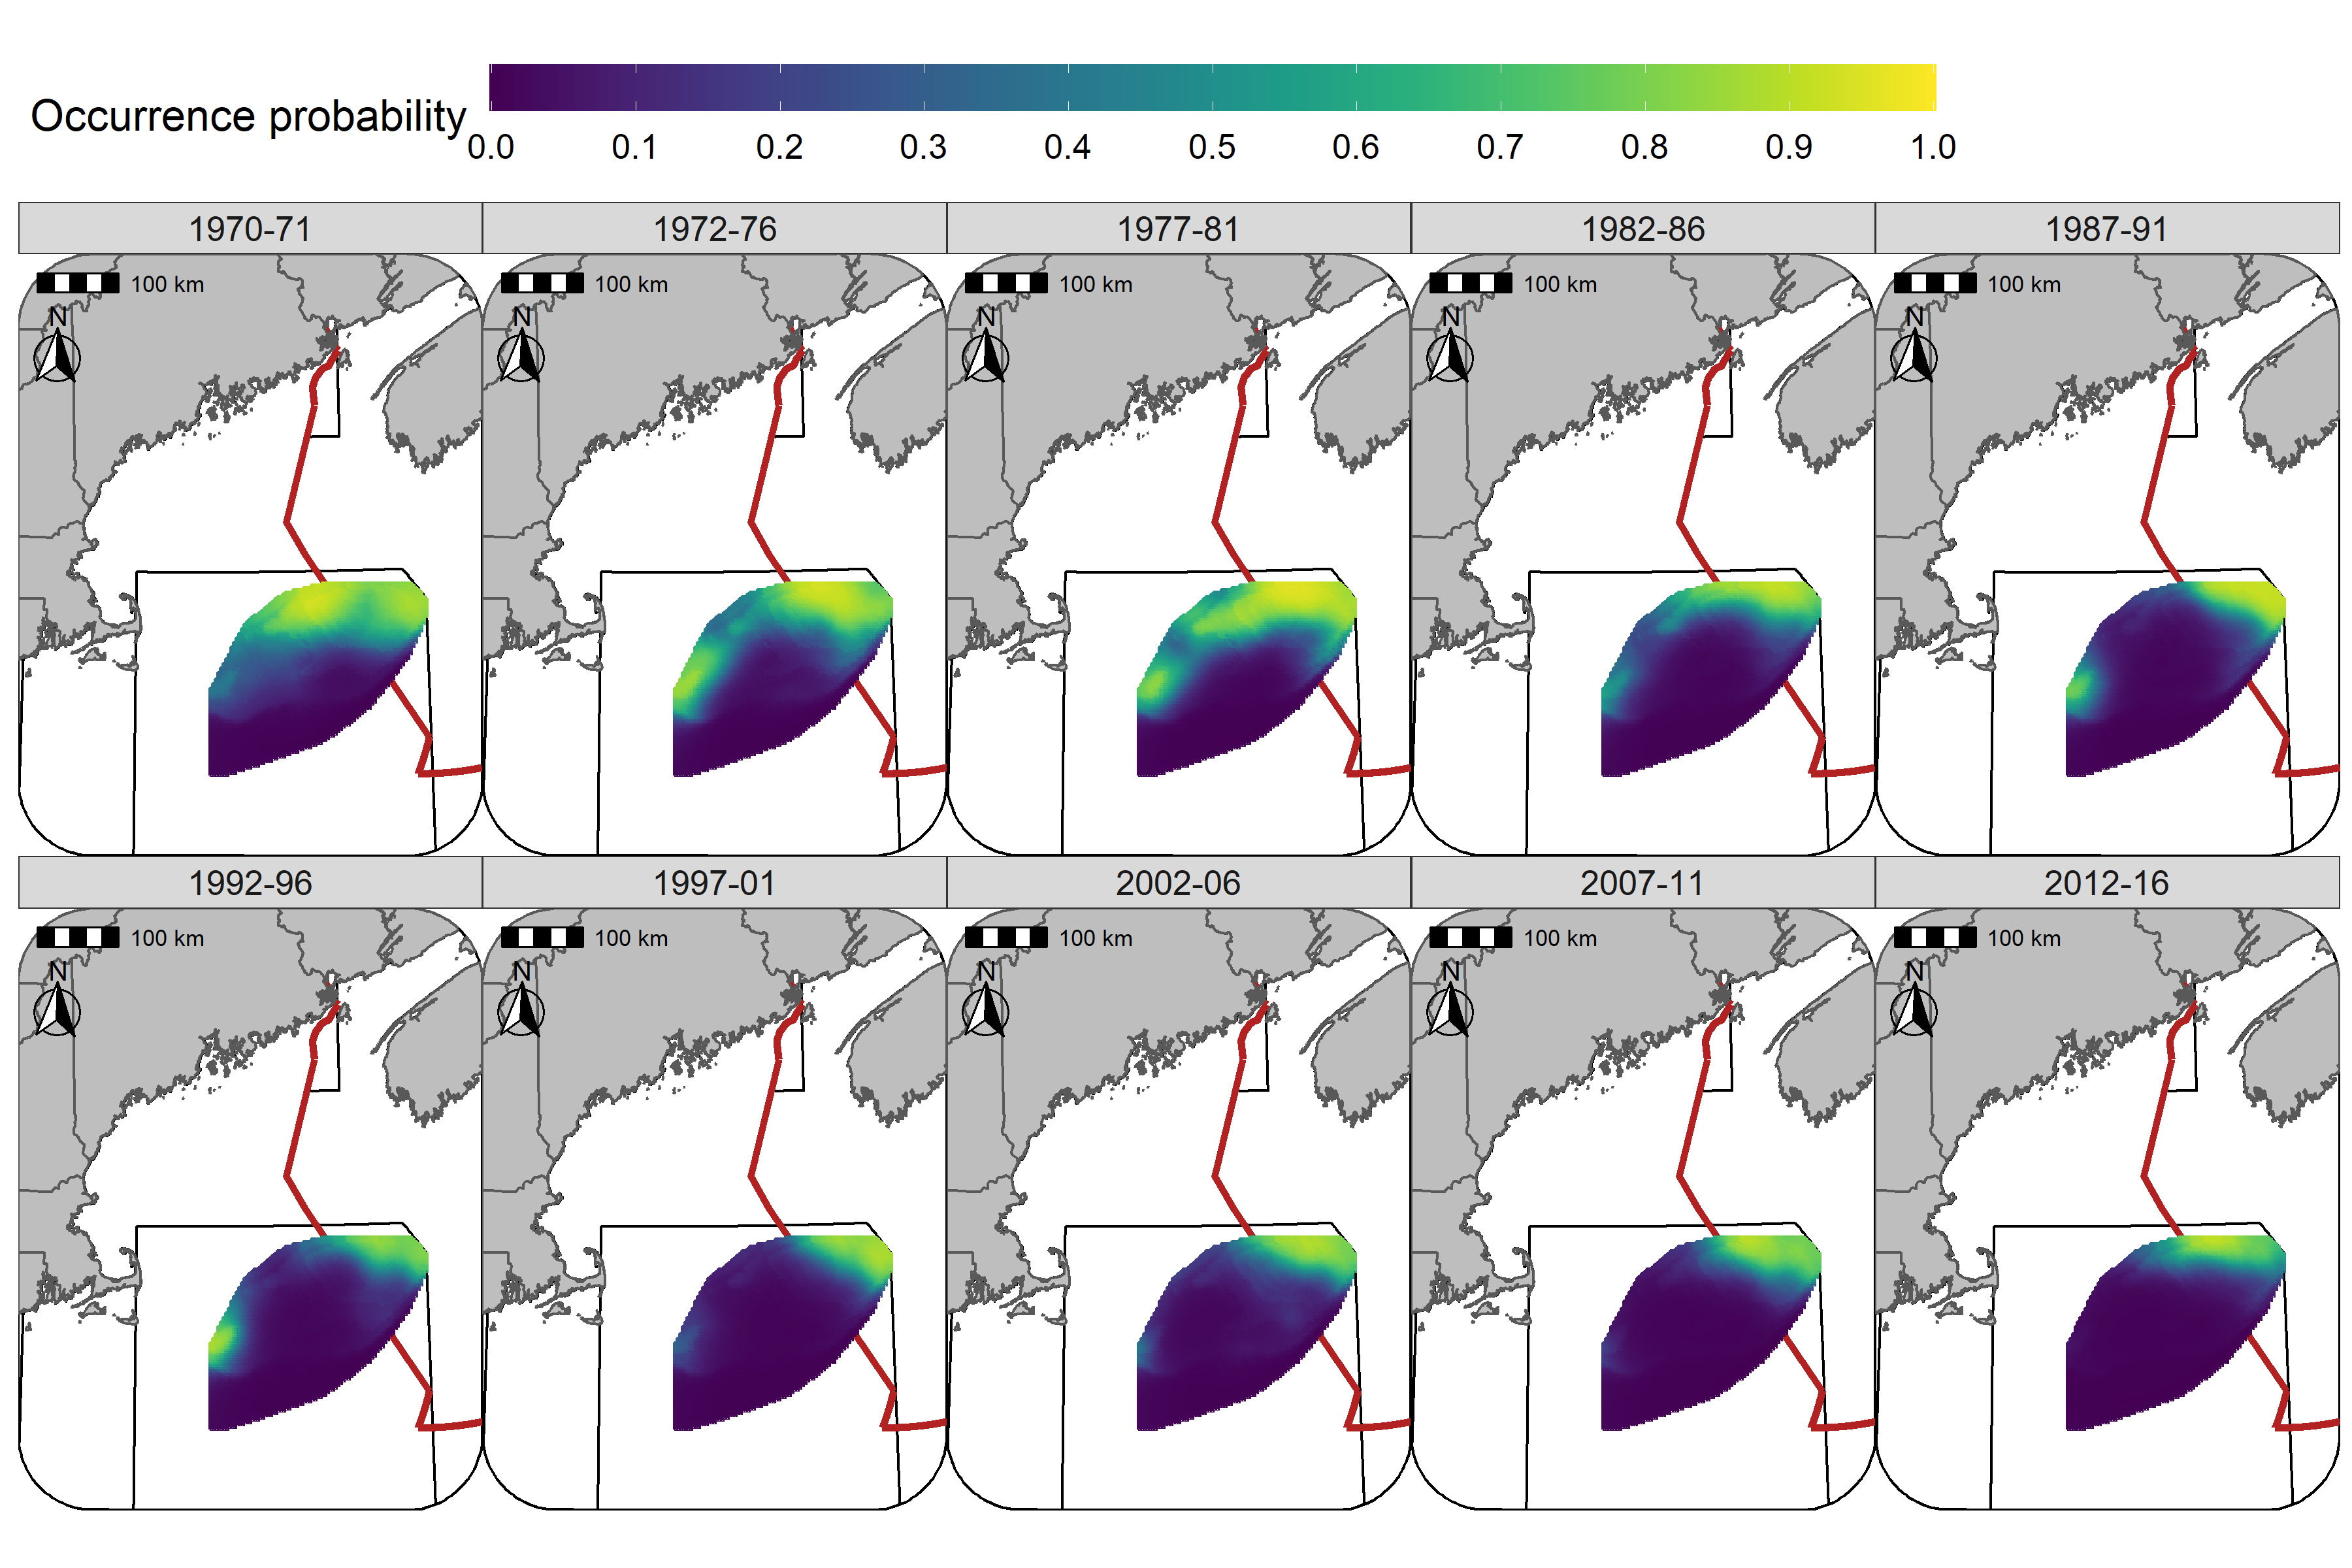
\includegraphics[width=1\linewidth]{D:/Github/Paper_2_SDMs/Results/Figures/pf_fall_cod} \caption{Predicted occurrence probability for Atlantic Cod  in each era during the Fall (NMFS-fall survey) using the SST + Dep model and 5-year random field.}\label{fig:pf-fall-cod}
\end{figure}

\newpage
\begin{figure}
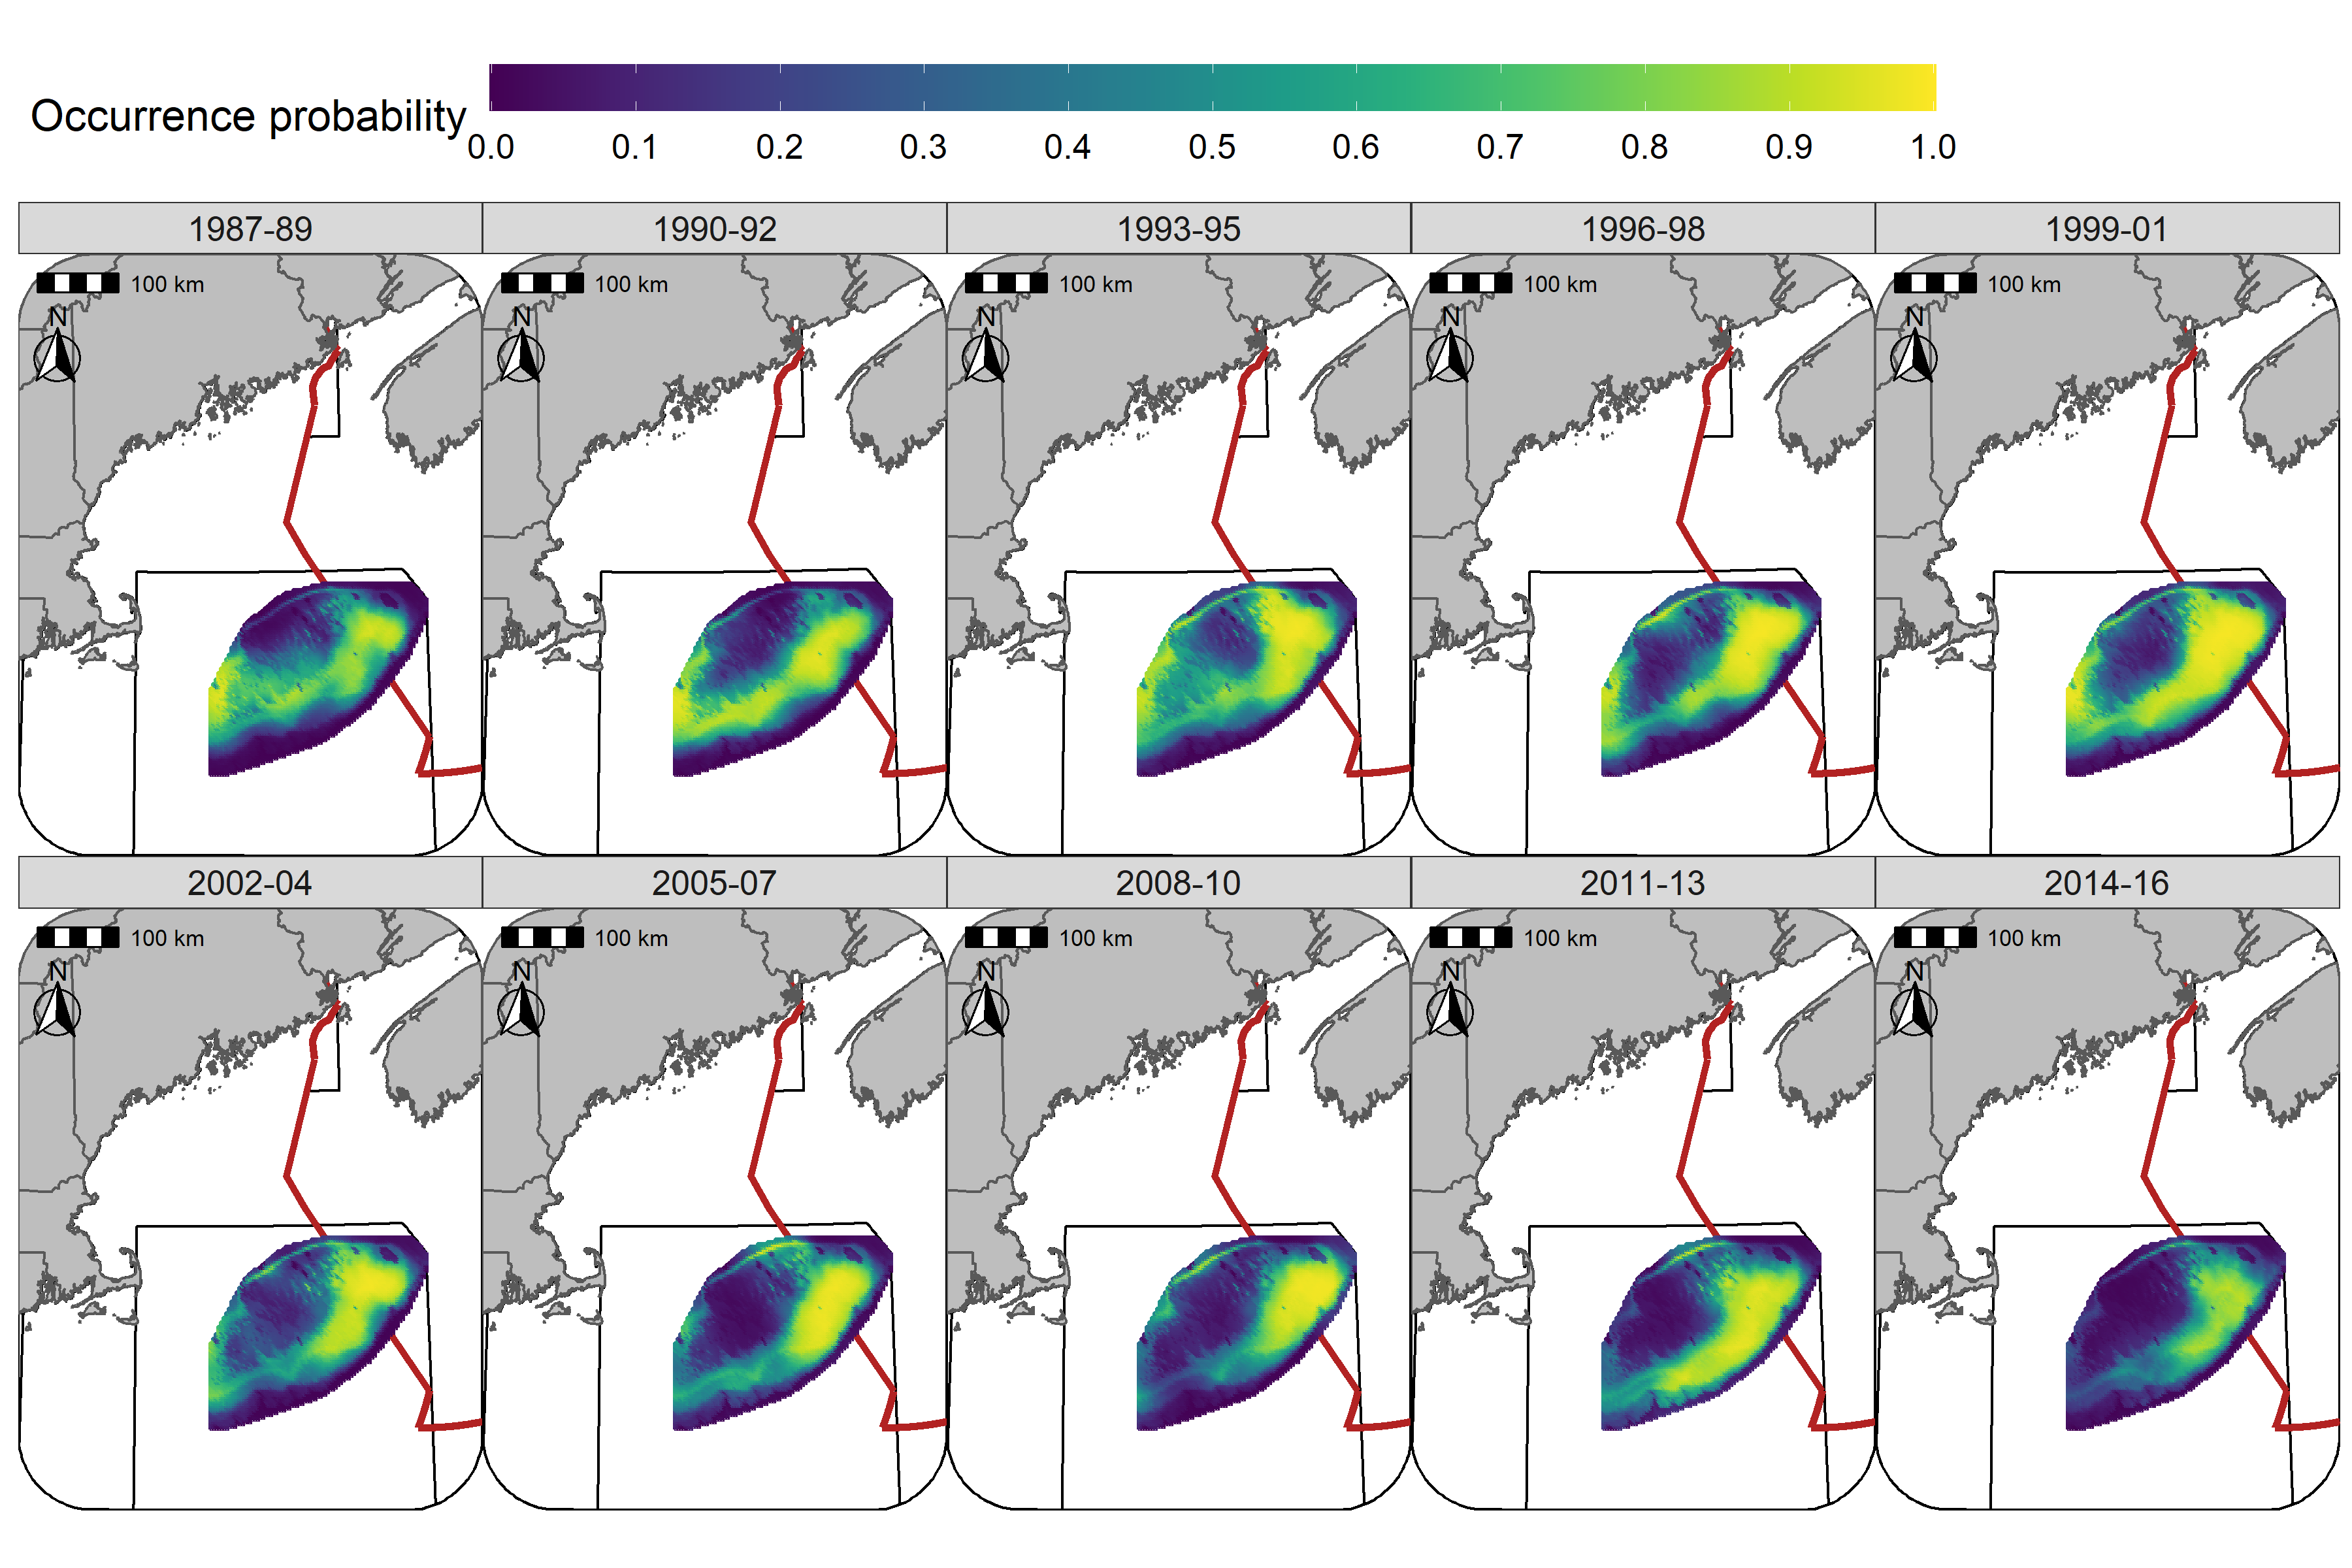
\includegraphics[width=1\linewidth]{D:/Github/Paper_2_SDMs/Results/Figures/pf_winter_yt} \caption{Predicted occurrence probability for Yellowtail Flounder in each era during the Winter (RV survey) using the SST + Dep + Sed model and 3-year random field.}\label{fig:pf-winter-yt}
\end{figure}

\newpage
\begin{figure}
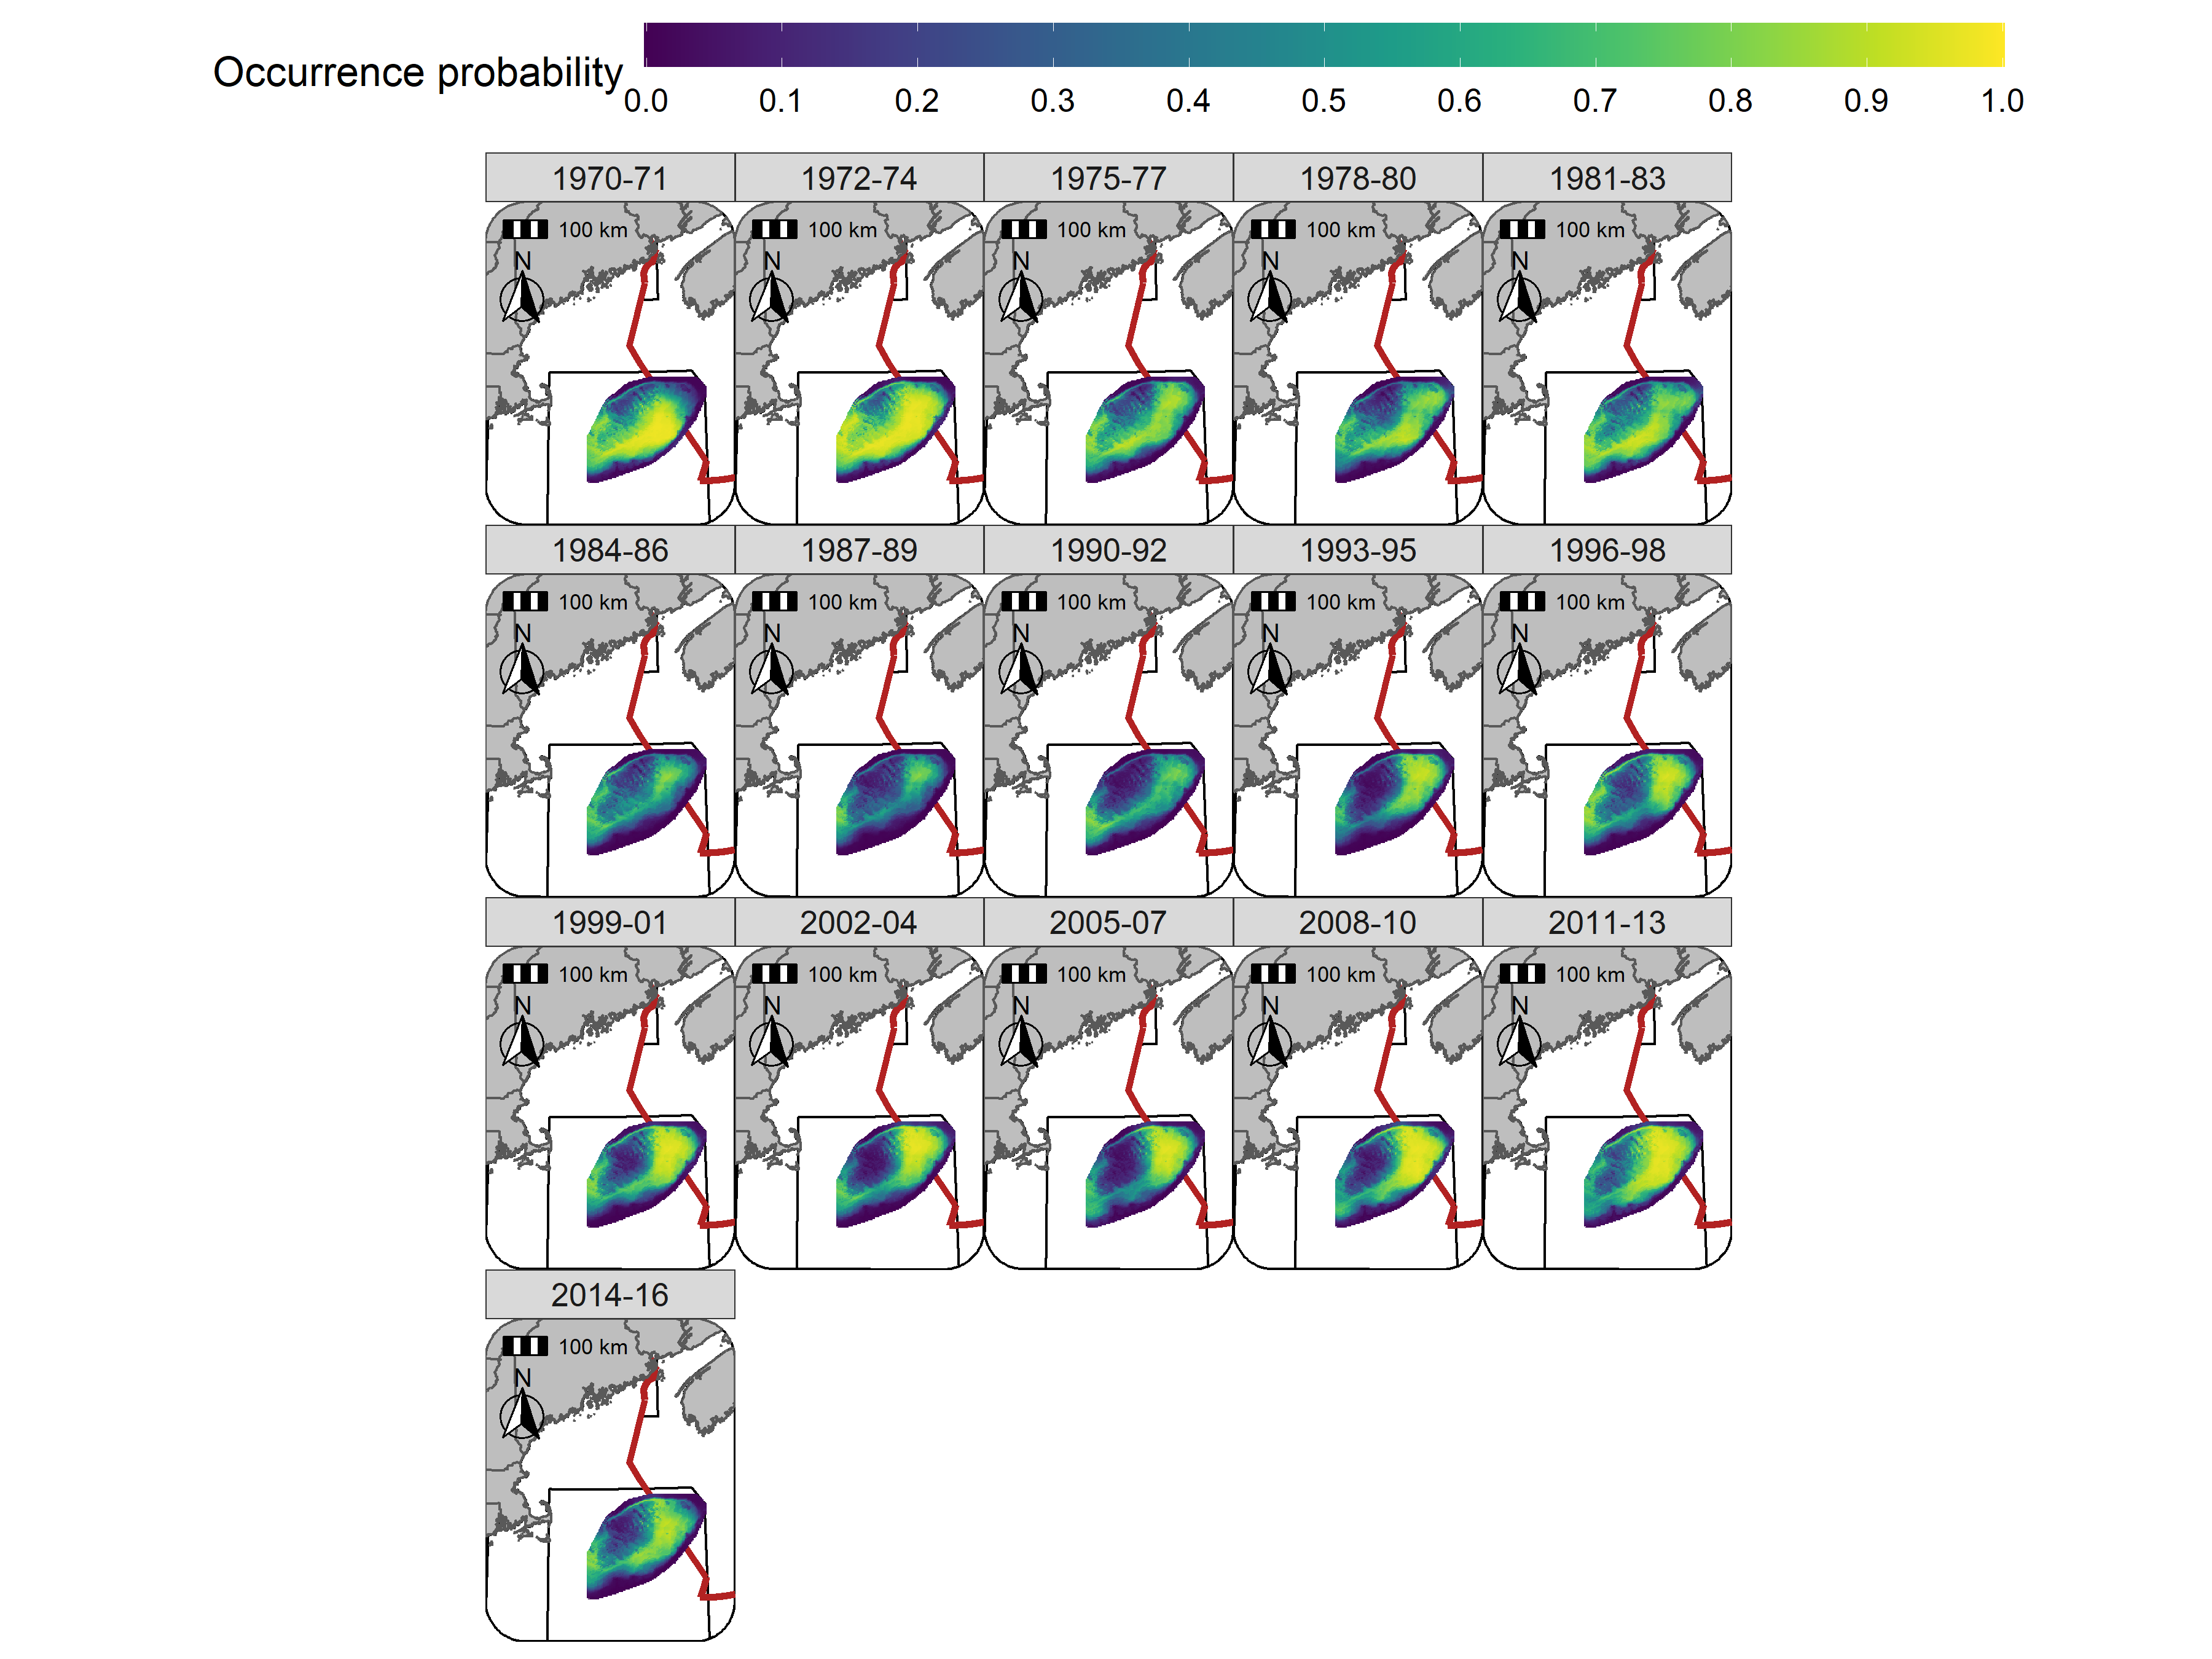
\includegraphics[width=1\linewidth]{D:/Github/Paper_2_SDMs/Results/Figures/pf_spring_yt} \caption{Predicted occurrence probability for Yellowtail Flounder in each era during the Spring (NMFS-spring survey) using the SST + Dep + Sed  model and 3-year random field.}\label{fig:pf-spring-yt}
\end{figure}

\newpage
\begin{figure}
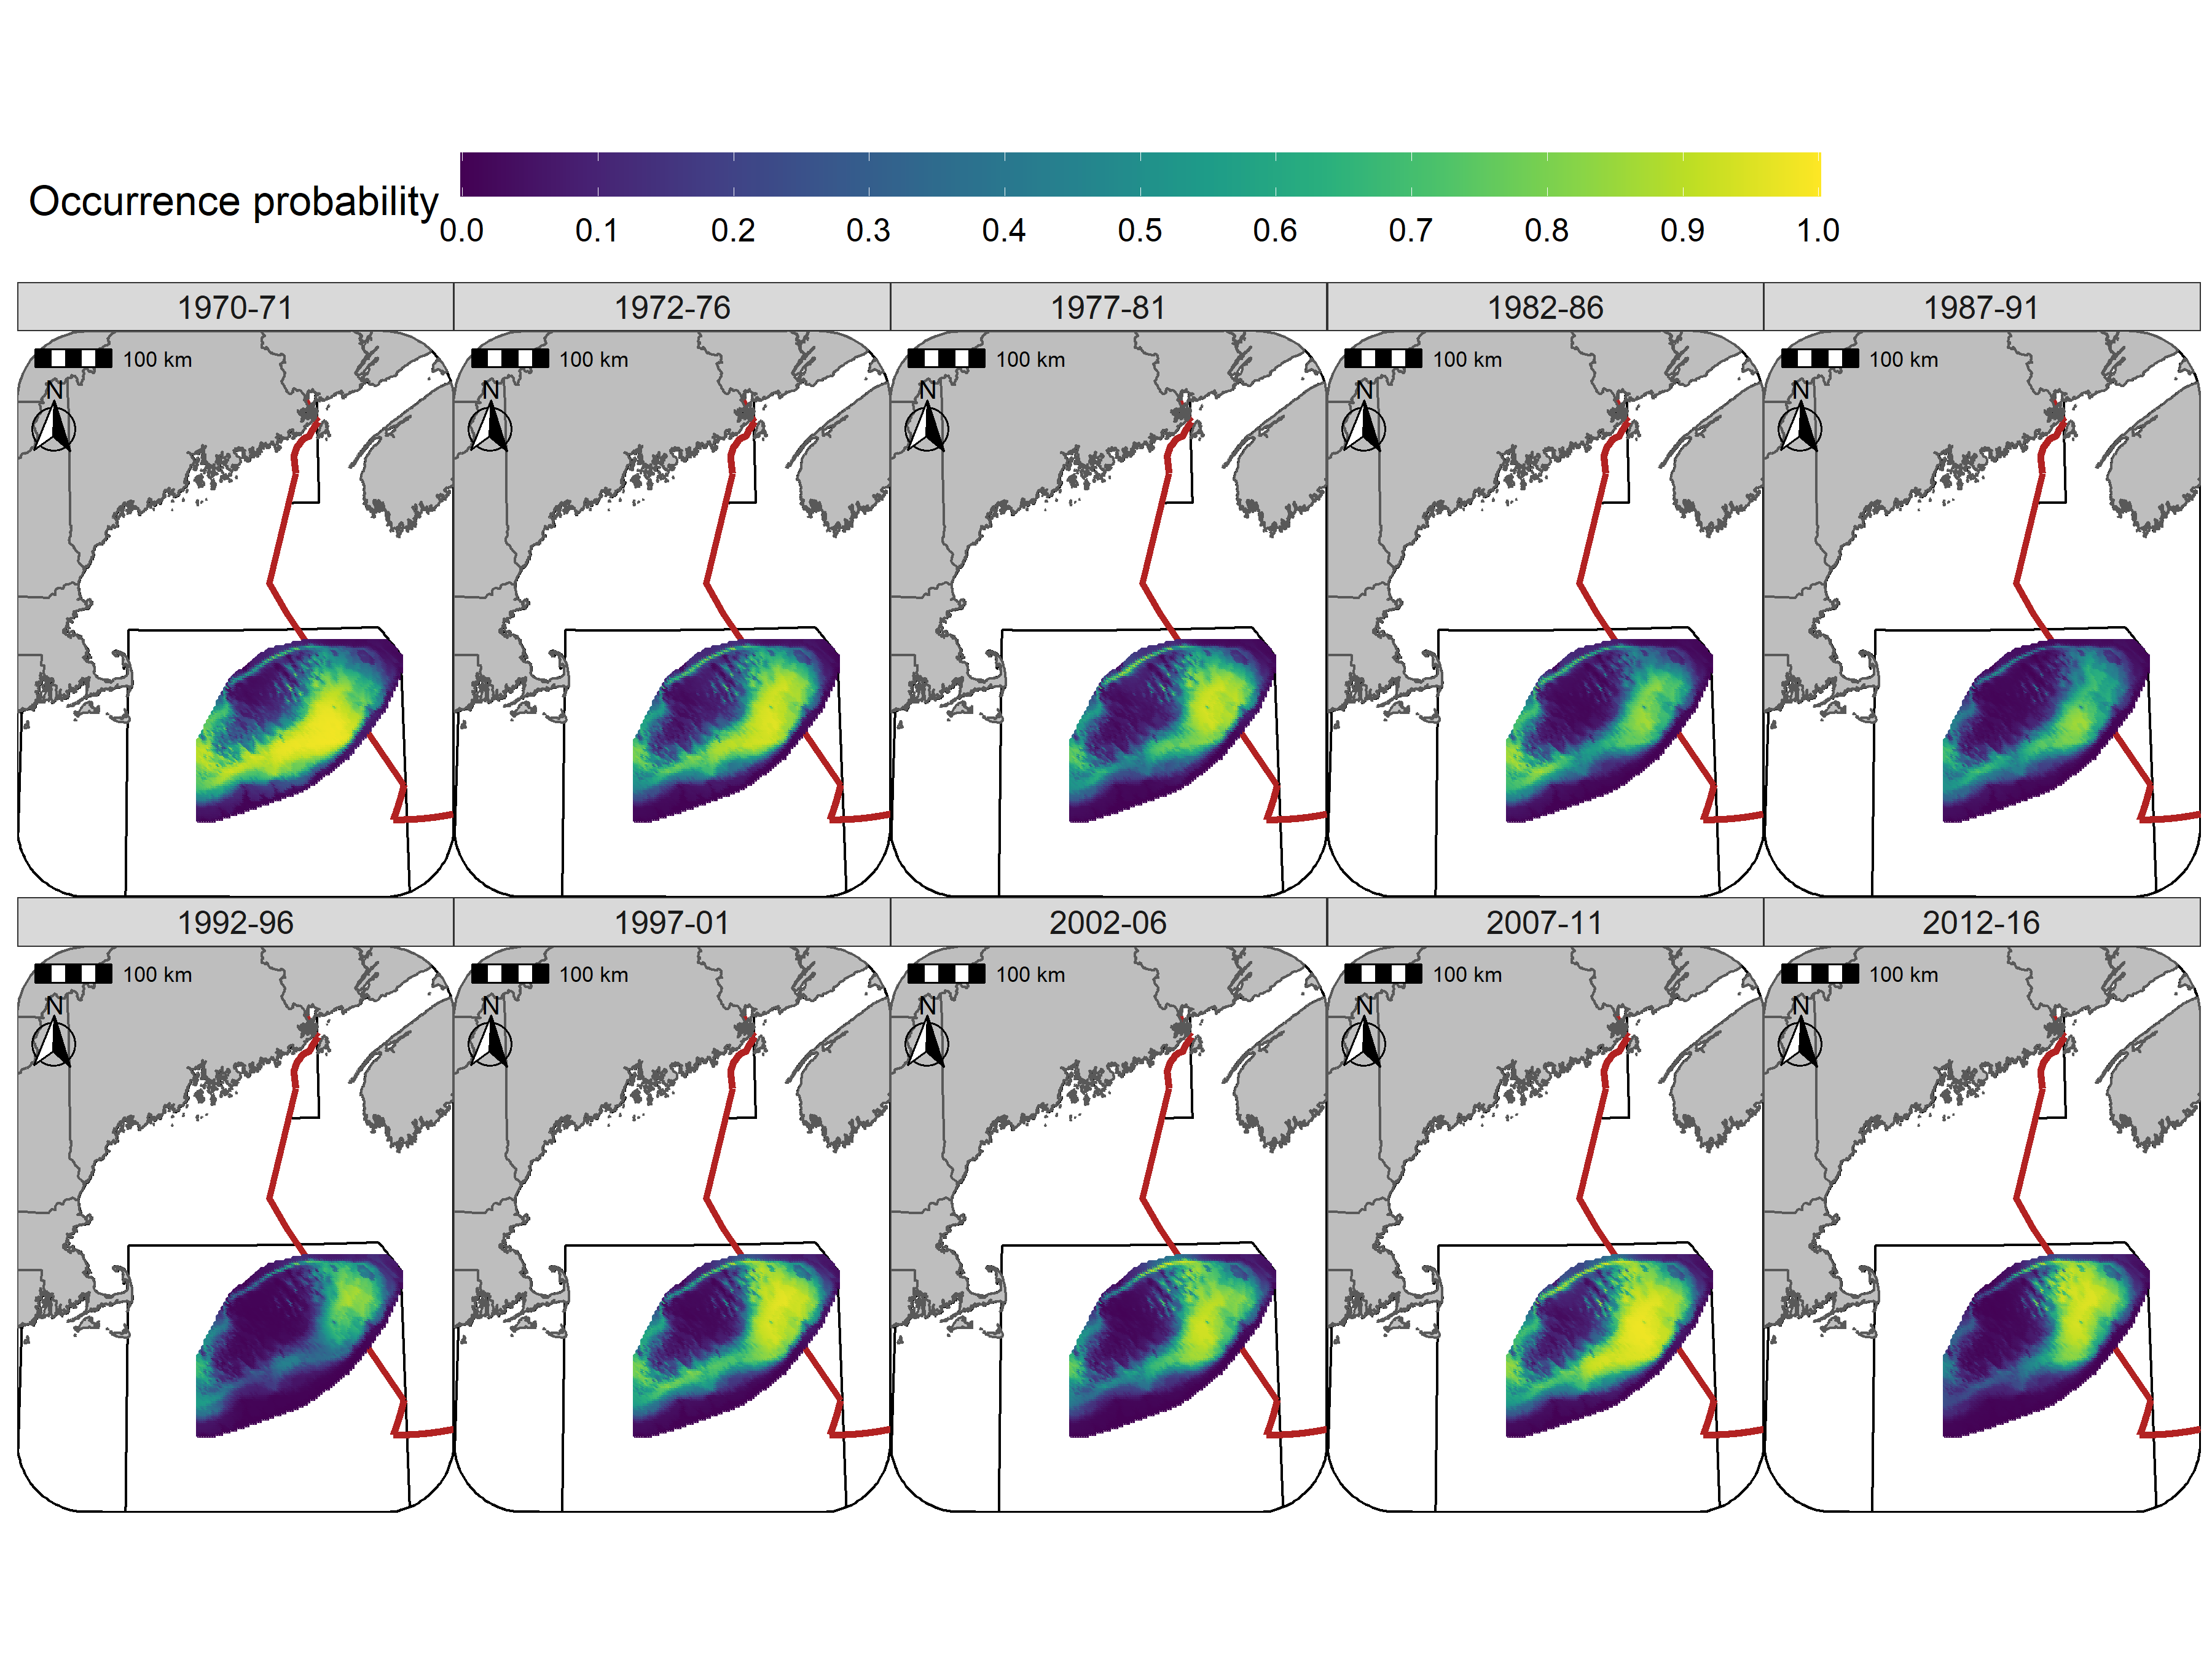
\includegraphics[width=1\linewidth]{D:/Github/Paper_2_SDMs/Results/Figures/pf_fall_yt} \caption{Predicted occurrence probability for Yellowtail Flounder in each era during the Fall (NMFS-fall survey) using the SST + Dep + Sed model and 5-year random field.}\label{fig:pf-fall-yt}
\end{figure}

\newpage

\begin{figure}
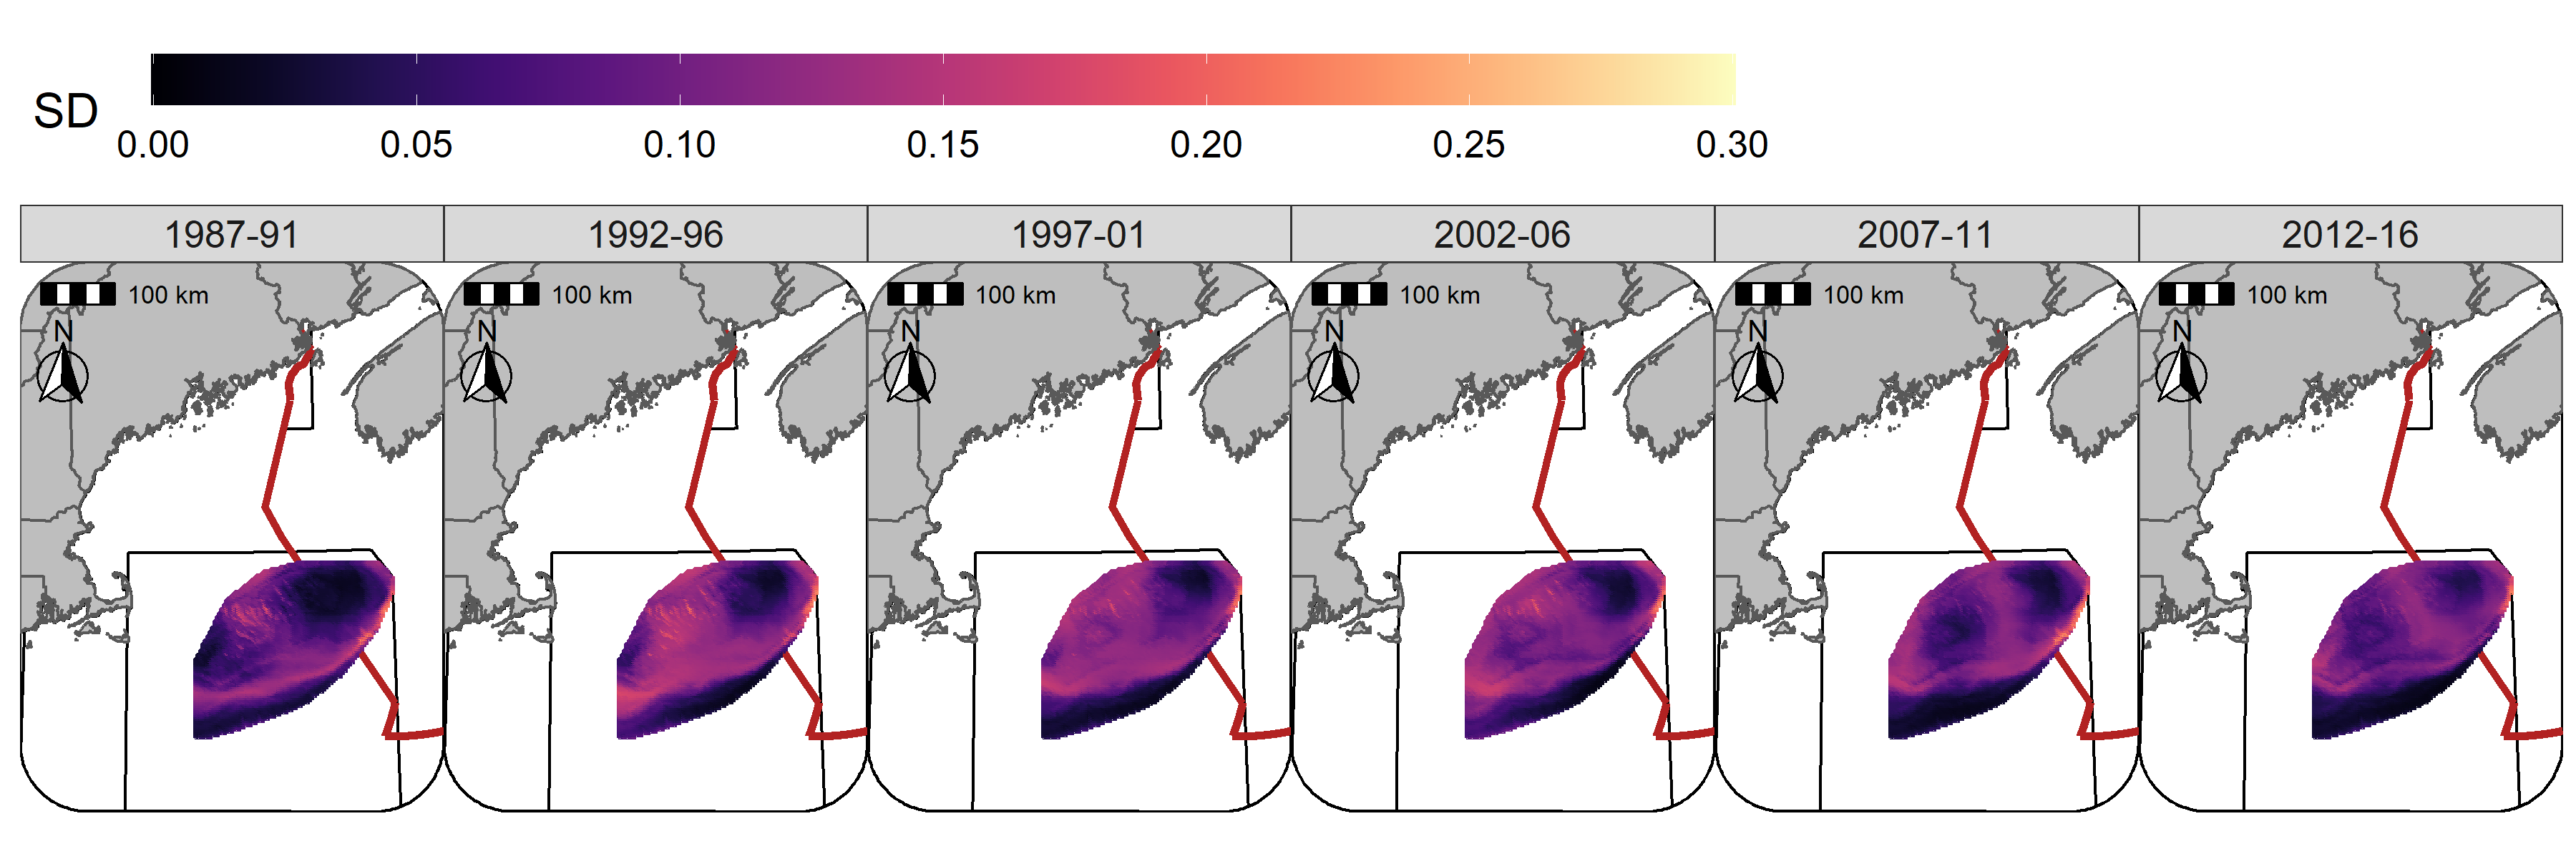
\includegraphics[width=1\linewidth]{D:/Github/Paper_2_SDMs/Results/Figures/pf_winter_cod_sd} \caption{Standard deviation (logit scale) of predicted occurrence probability for Atlantic Cod  in each era during the Winter (RV survey) using the SST + Dep model and 5-year random field.}\label{fig:pf-winter-cod-sd}
\end{figure}

\newpage
\begin{figure}
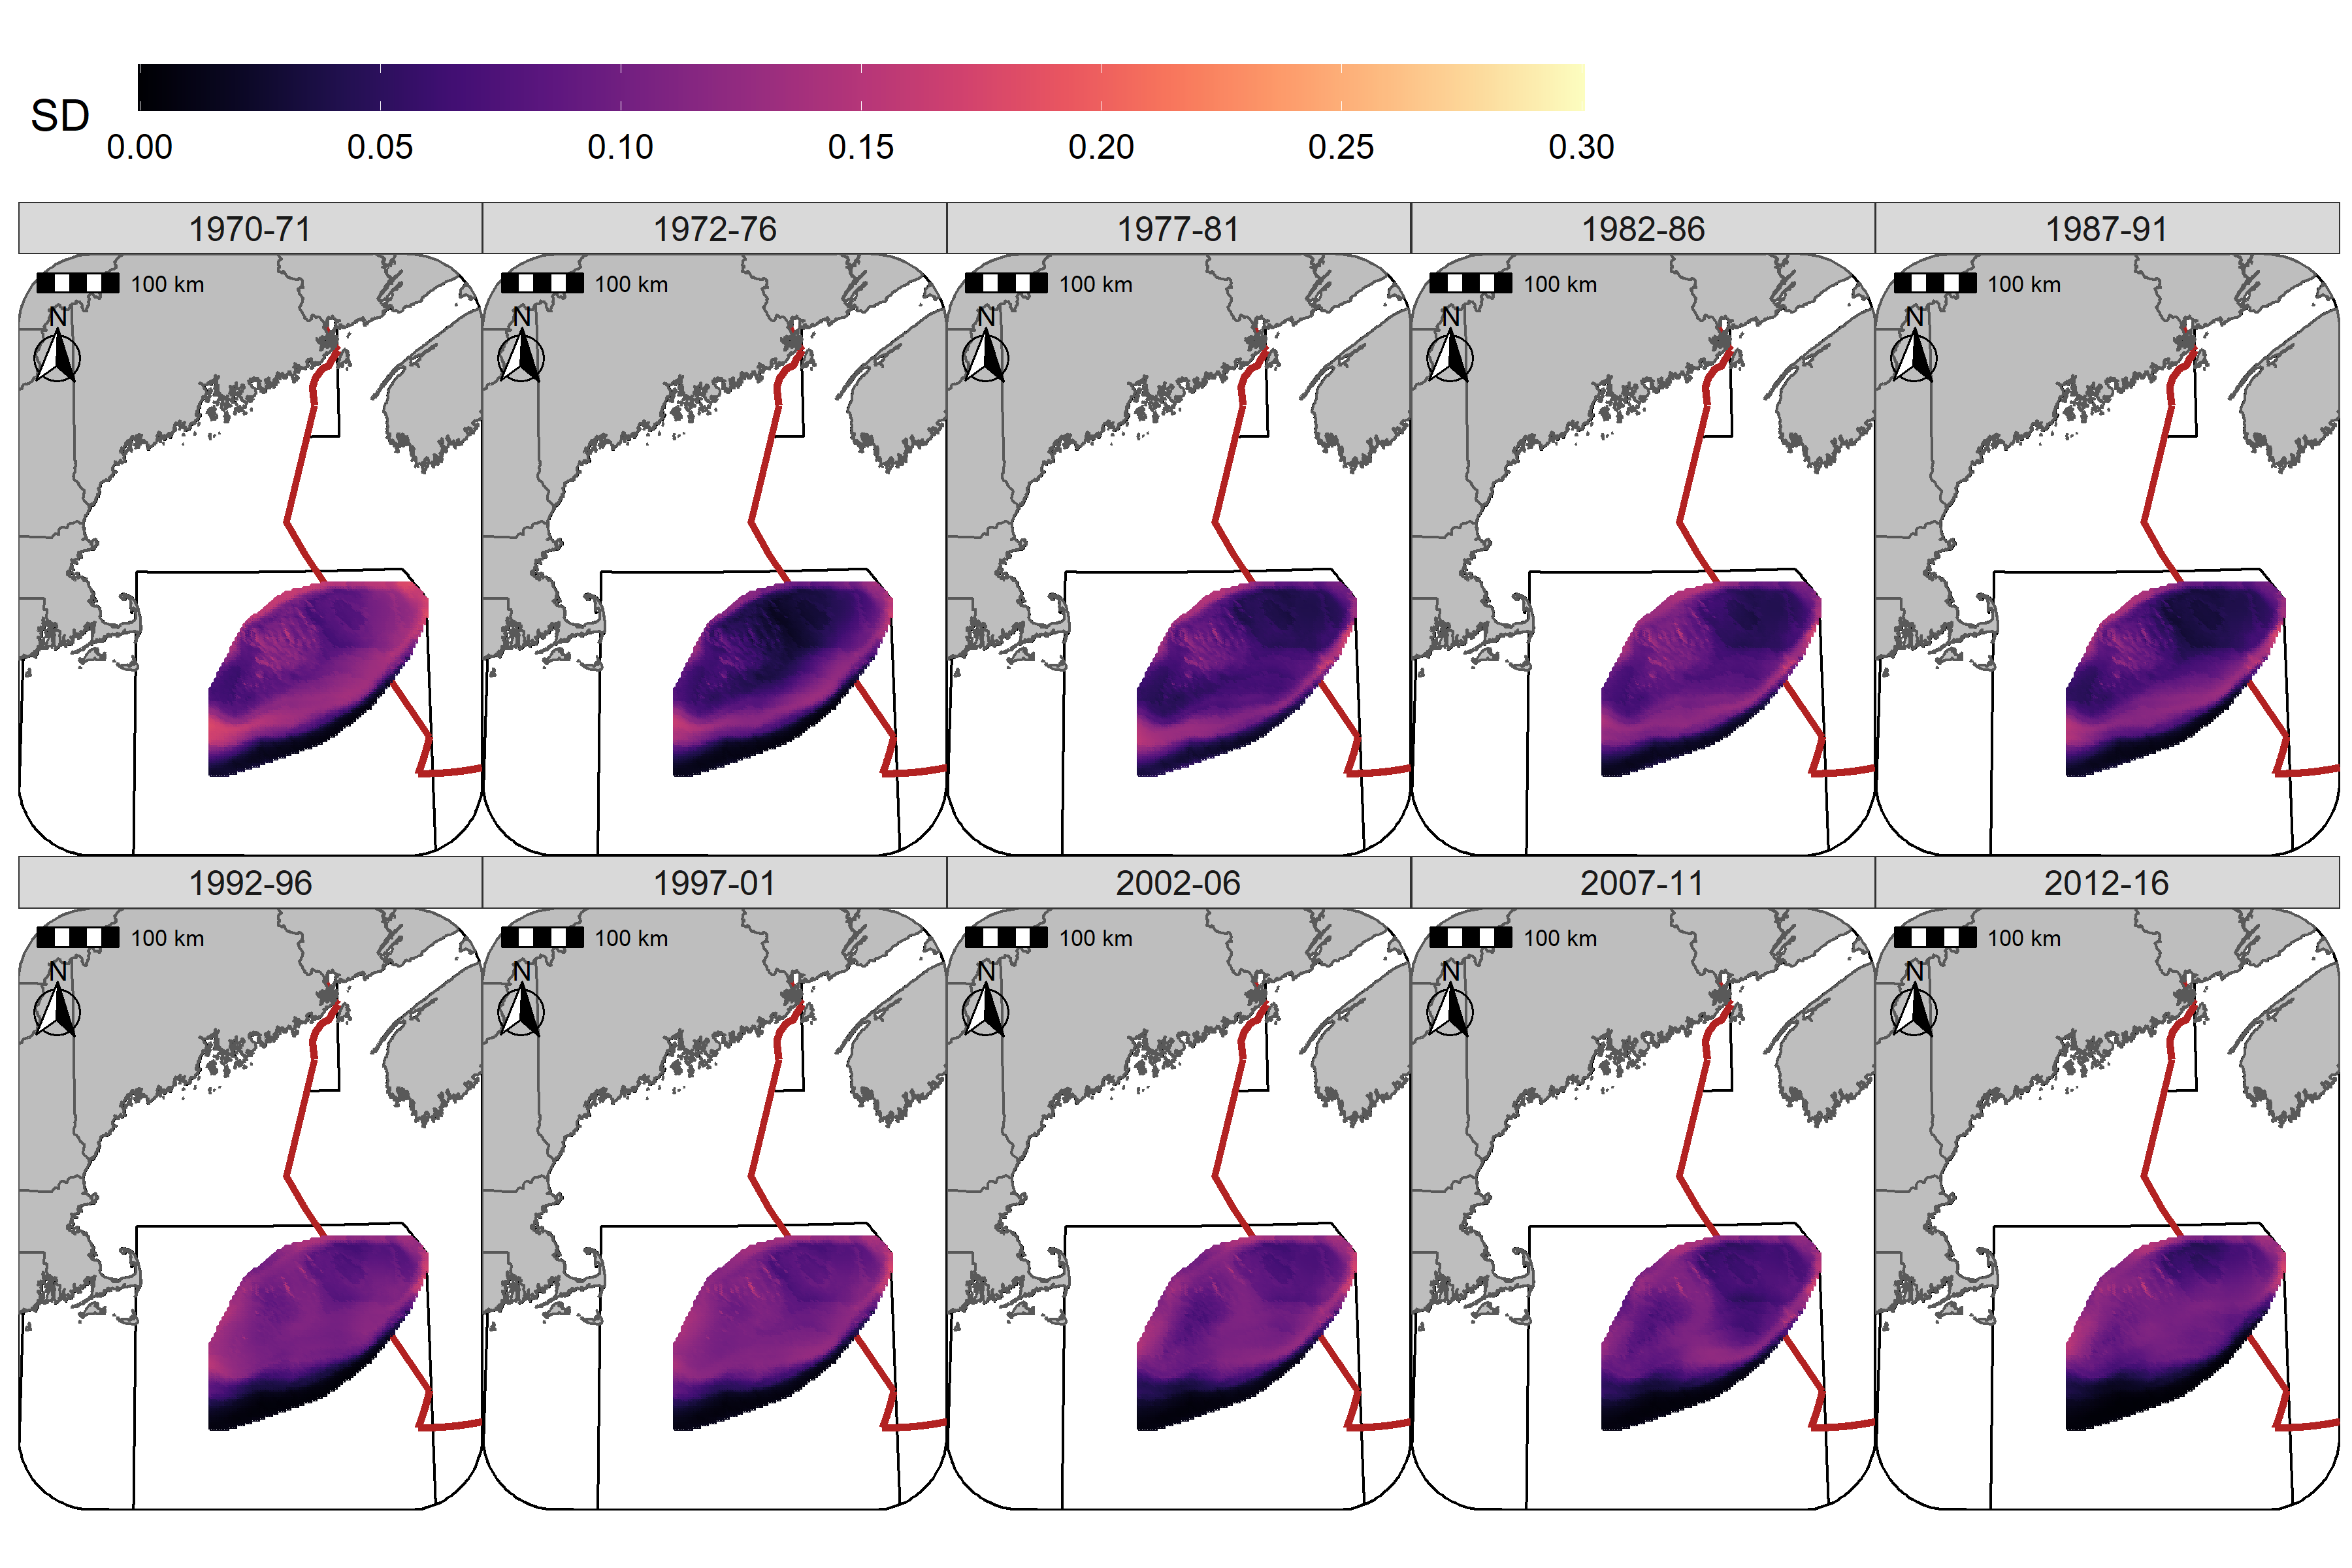
\includegraphics[width=1\linewidth]{D:/Github/Paper_2_SDMs/Results/Figures/pf_spring_cod_sd} \caption{Standard deviation (logit scale) of predicted occurrence probability for Atlantic Cod  in each era during the Spring (NMFS-spring survey) using the SST + Dep model and 5-year random field.}\label{fig:pf-spring-cod-sd}
\end{figure}

\newpage
\begin{figure}
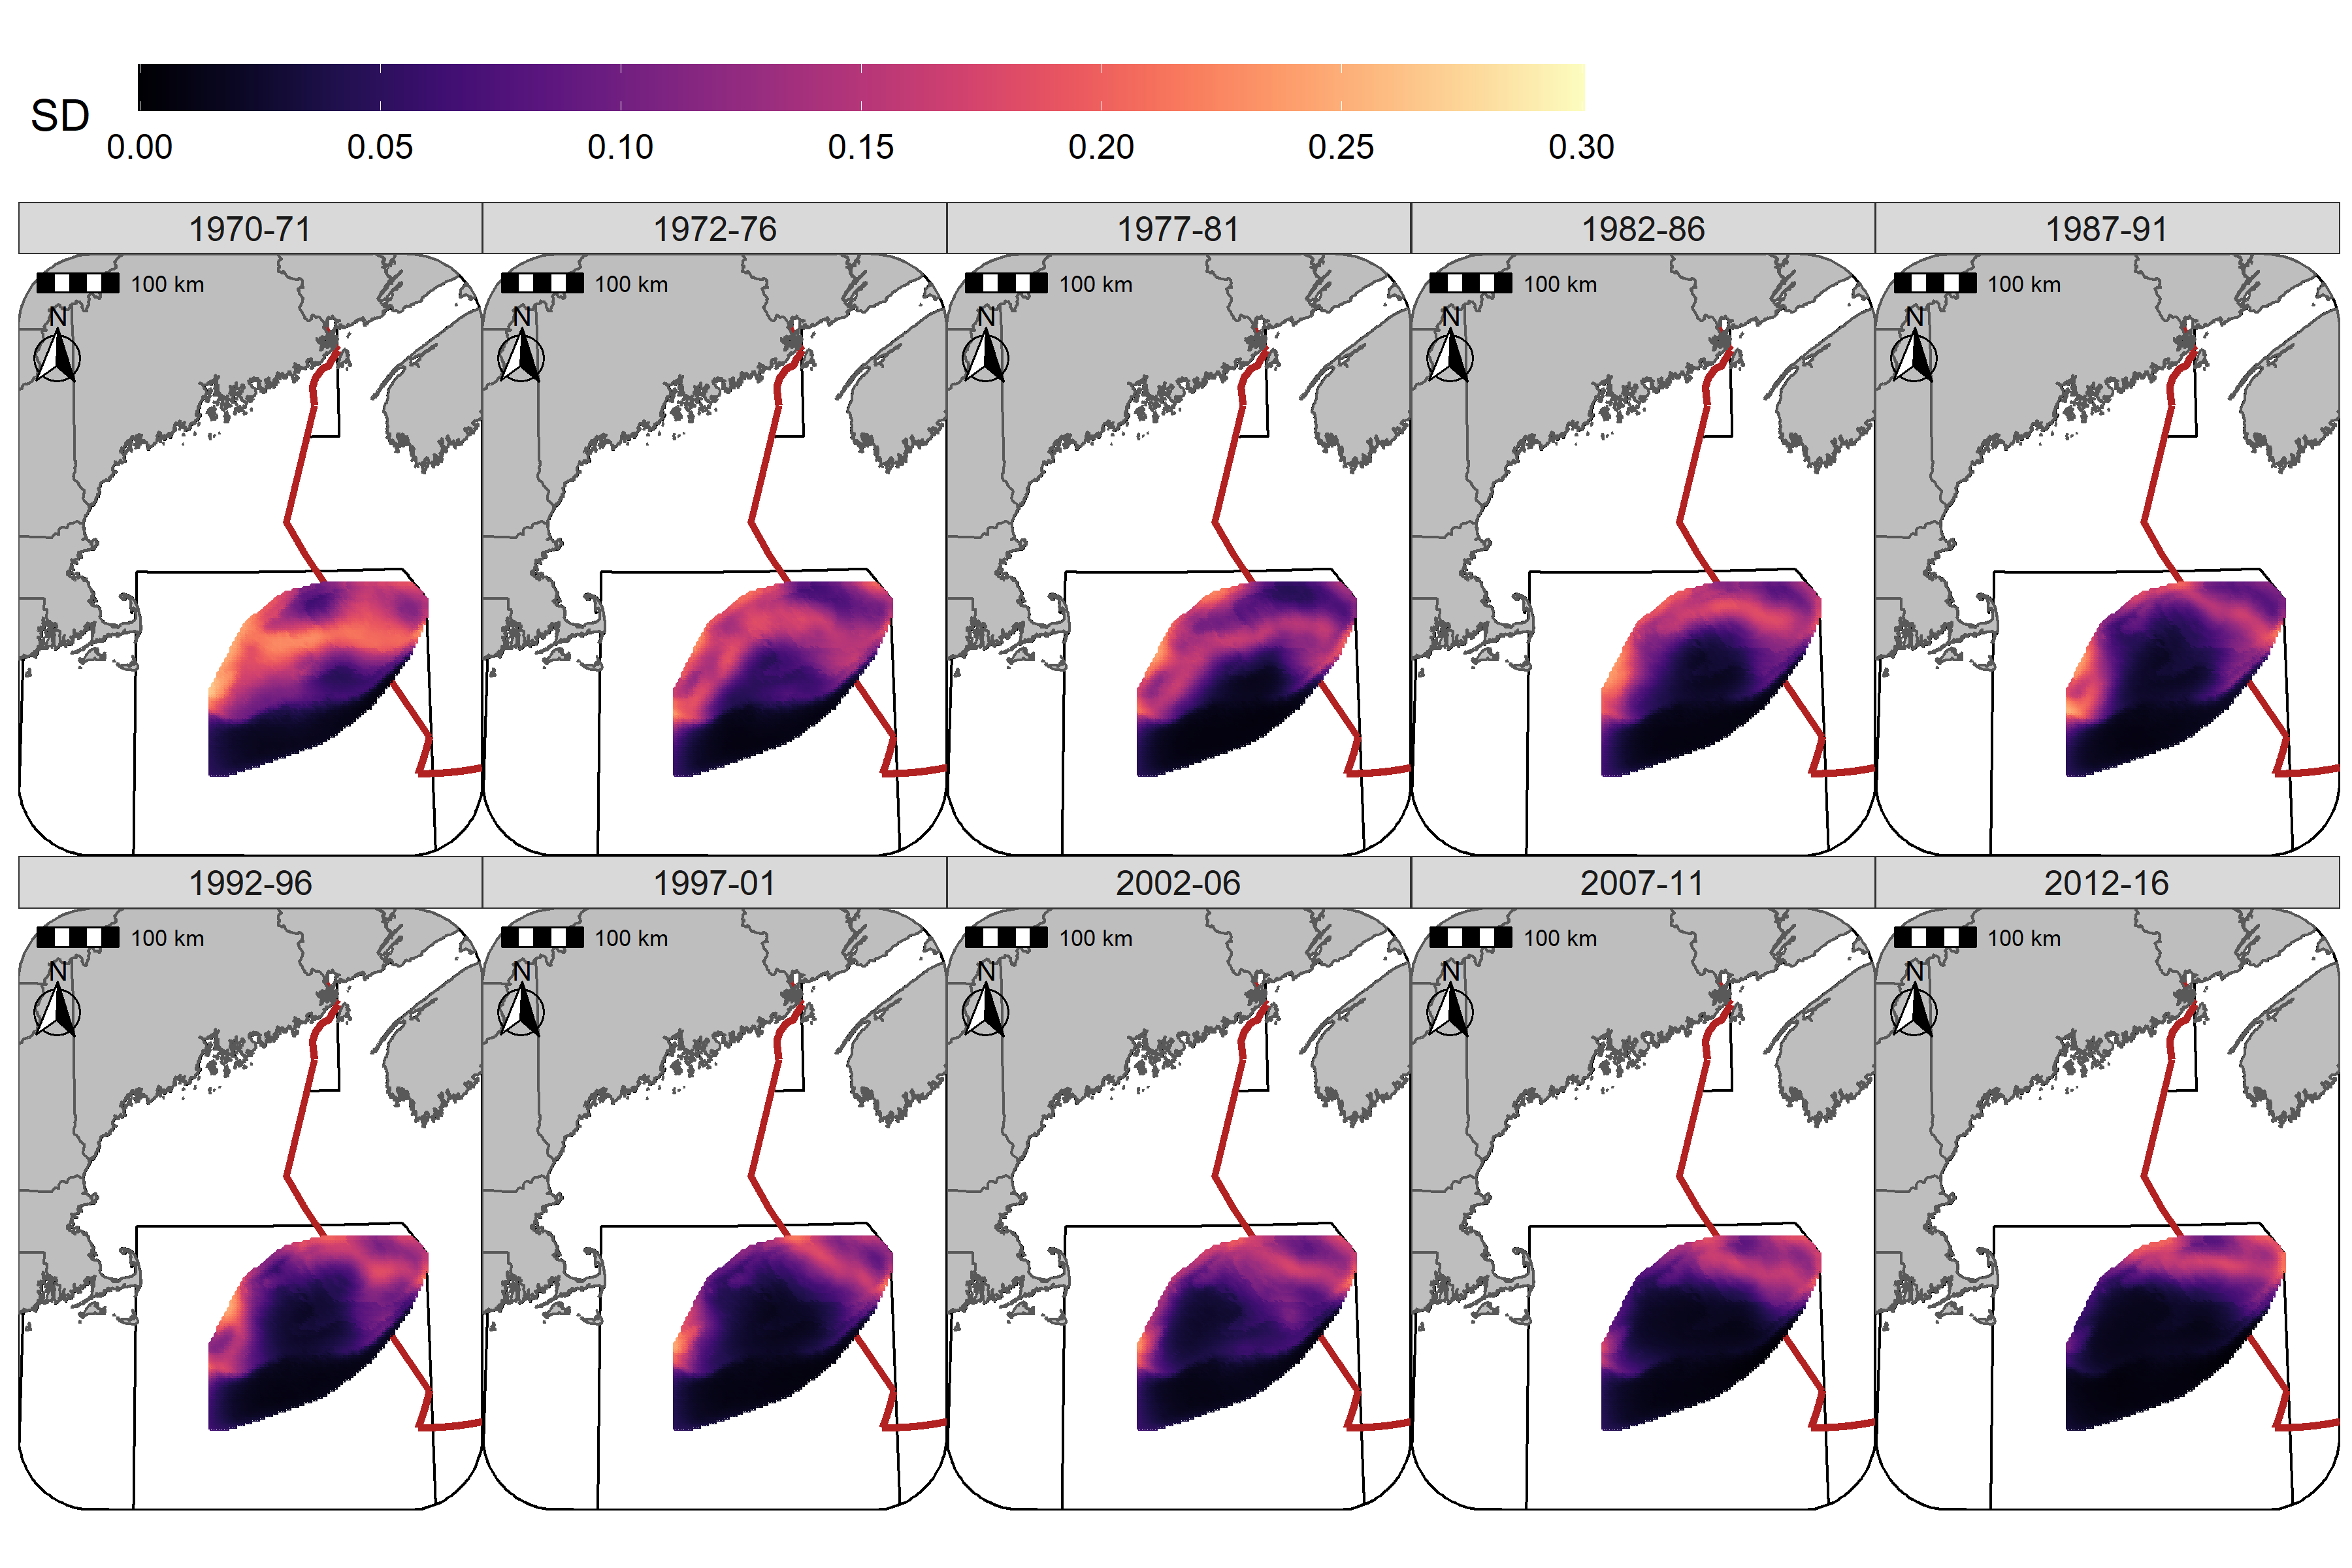
\includegraphics[width=1\linewidth]{D:/Github/Paper_2_SDMs/Results/Figures/pf_fall_cod_sd} \caption{Standard deviation (logit scale) of predicted occurrence probability for Atlantic Cod  in each era during the Fall (NMFS-fall survey) using the SST + Dep model and 5-year random field.}\label{fig:pf-fall-cod-sd}
\end{figure}

\newpage
\begin{figure}
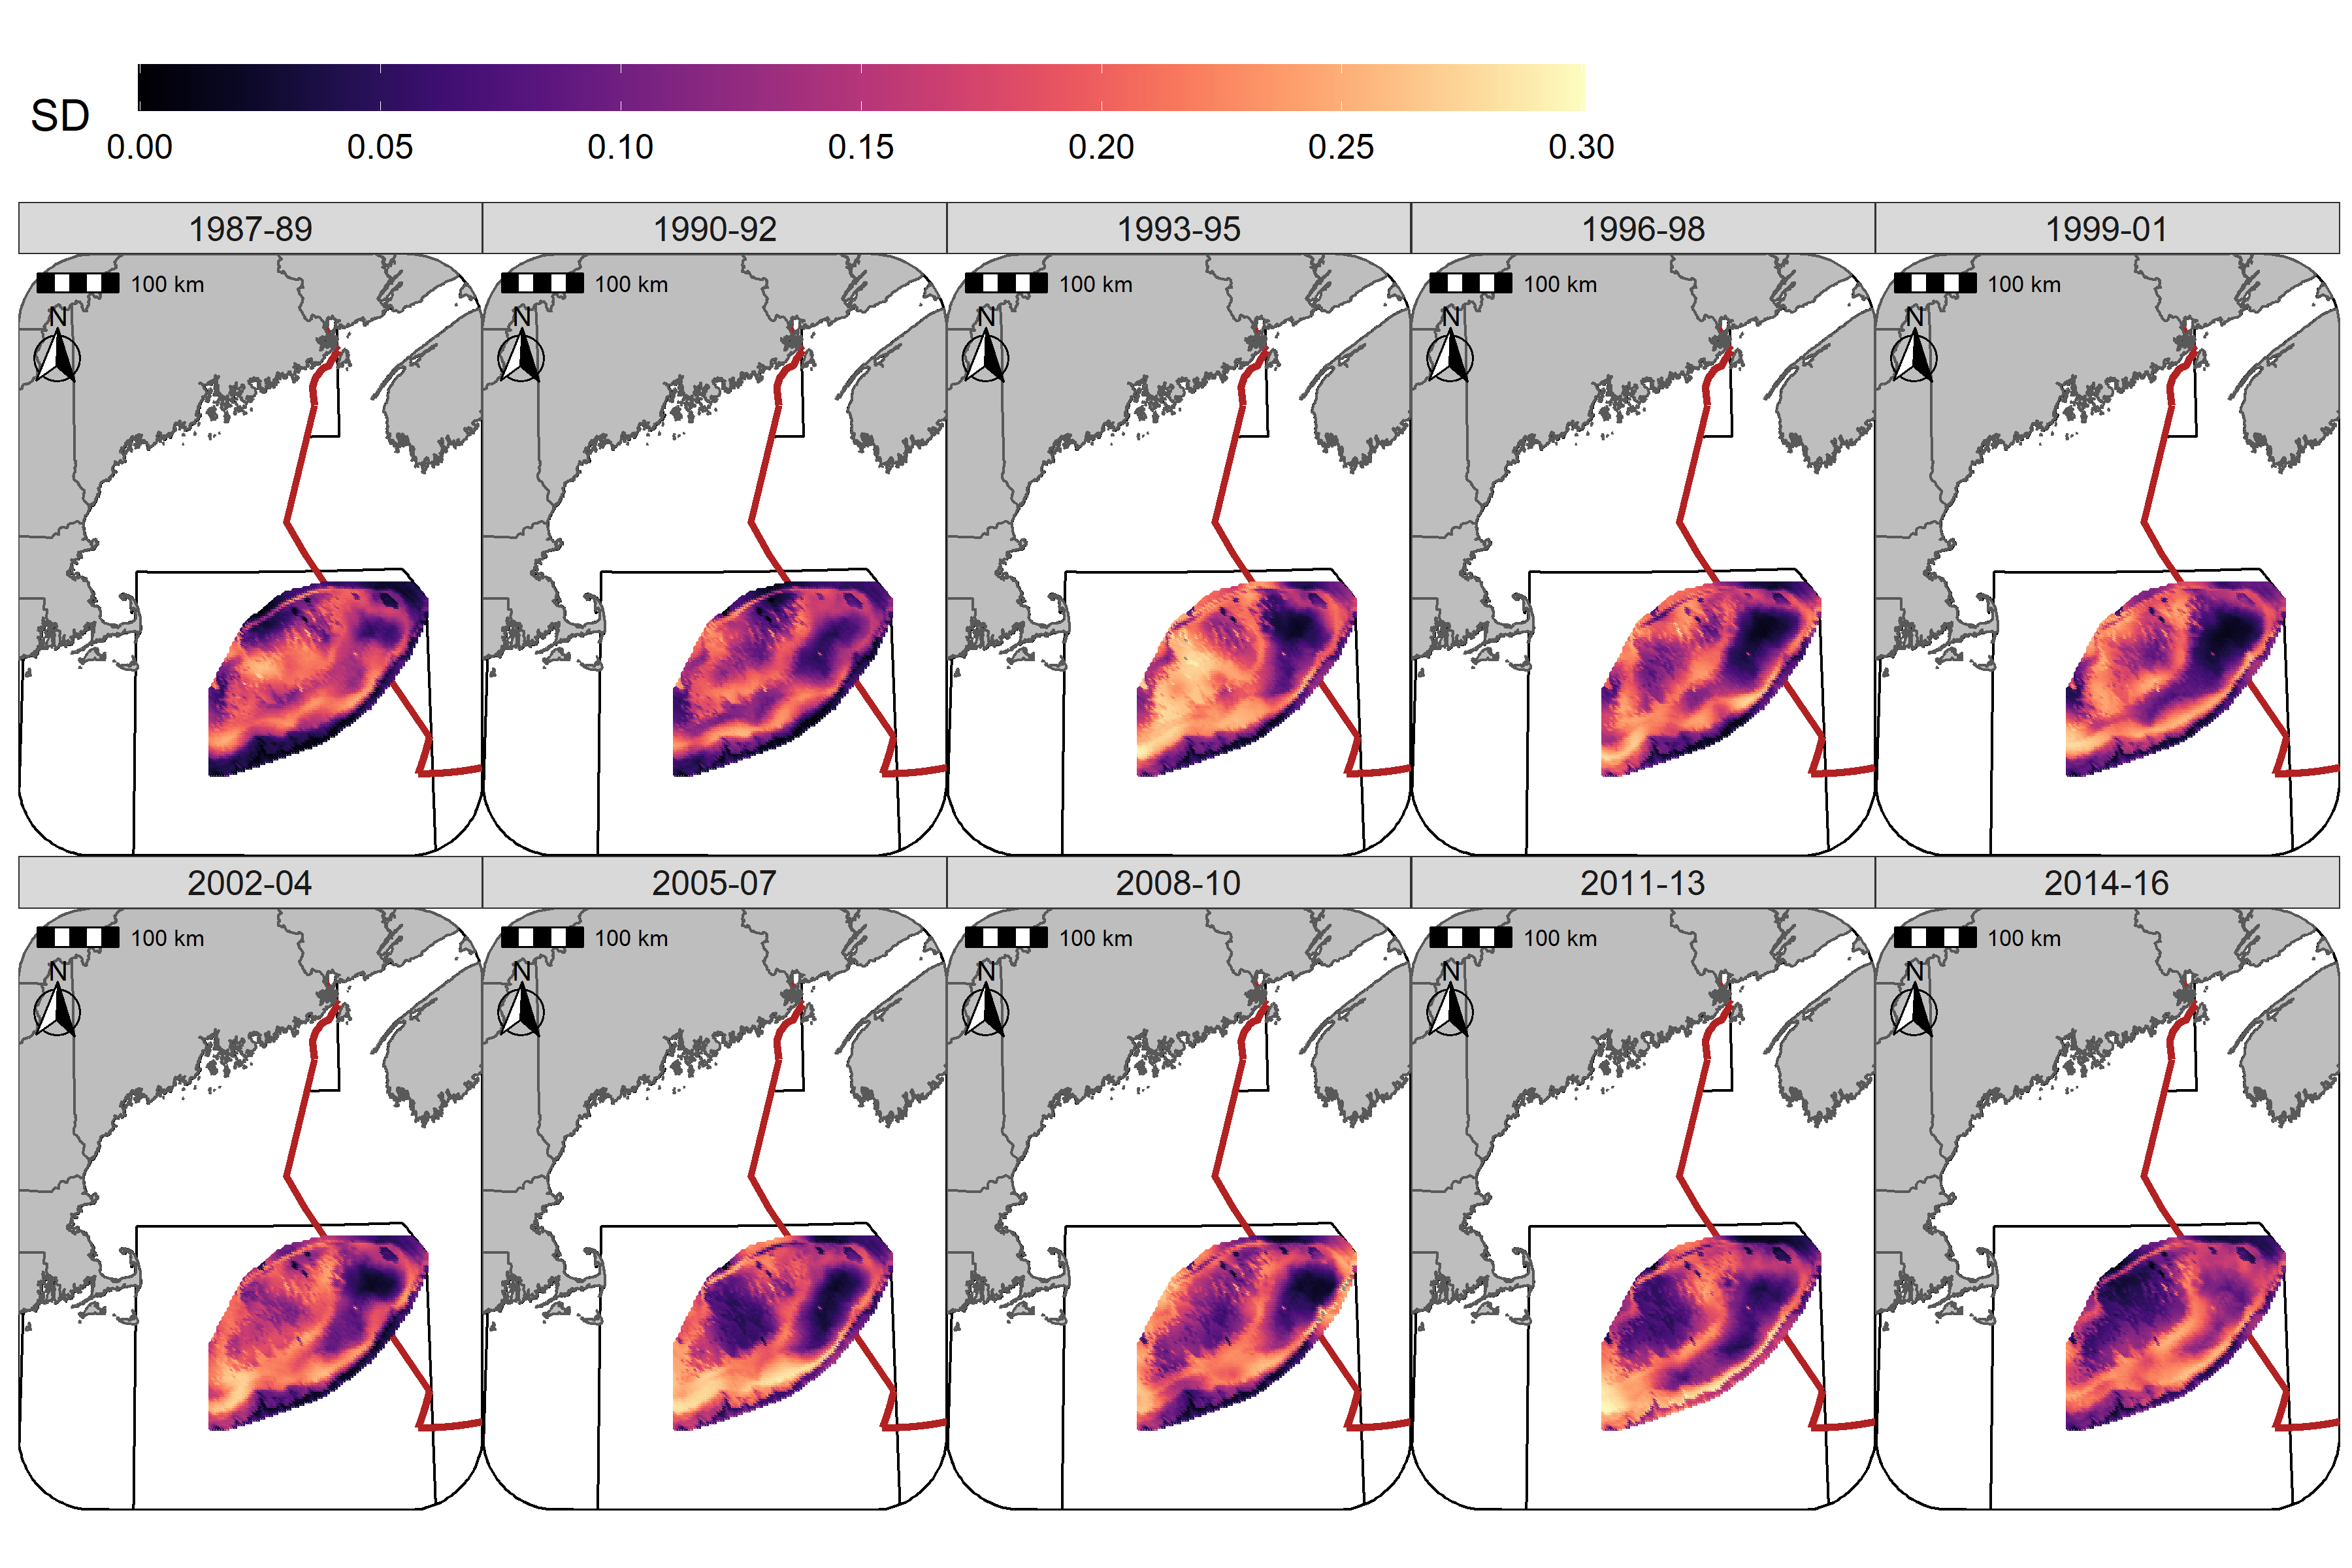
\includegraphics[width=1\linewidth]{D:/Github/Paper_2_SDMs/Results/Figures/pf_winter_yt_sd} \caption{Standard deviation (logit scale) of predicted occurrence probability for Yellowtail Flounder in each era during the Winter (RV survey) using the SST + Dep + Sed  model and 3-year random field.}\label{fig:pf-winter-yt-sd}
\end{figure}

\newpage

\begin{figure}
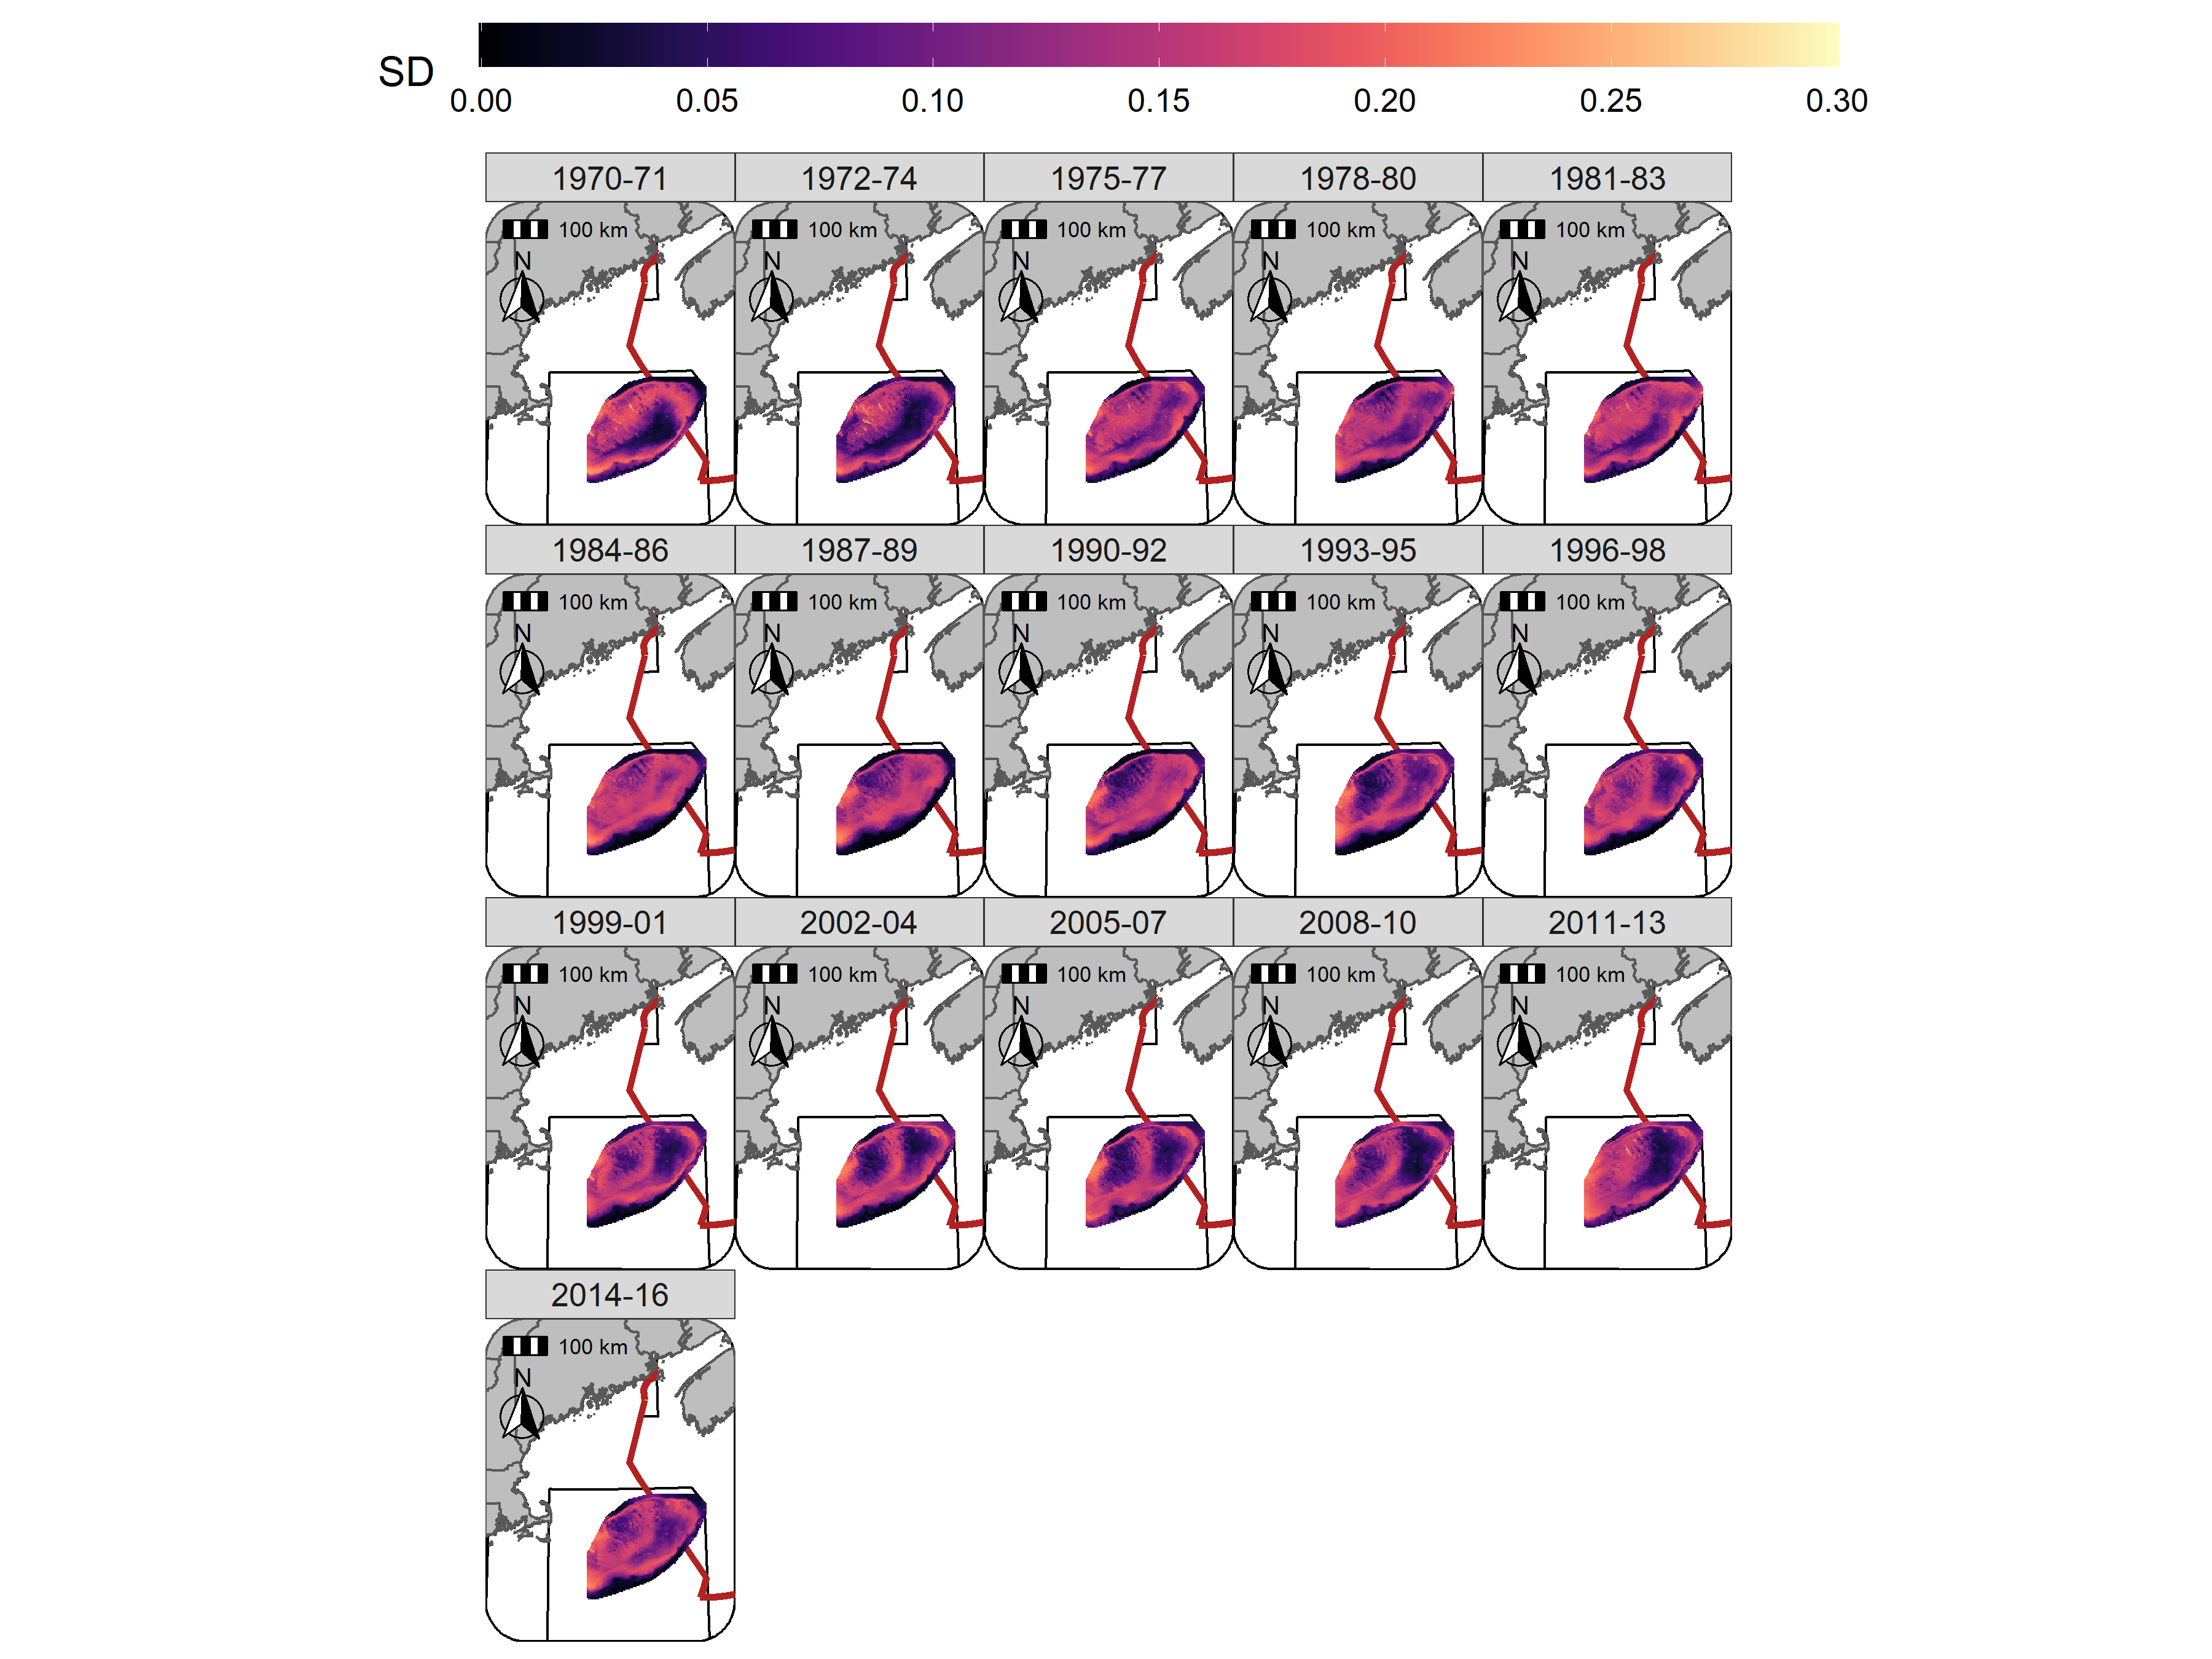
\includegraphics[width=1\linewidth]{D:/Github/Paper_2_SDMs/Results/Figures/pf_spring_yt_sd} \caption{Standard deviation (logit scale) of predicted occurrence probability for Yellowtail Flounder in each era during the Spring (NMFS-spring survey) using the  SST + Dep + Sed  model and 3-year random field.}\label{fig:pf-spring-yt-sd}
\end{figure}

\newpage
\begin{figure}
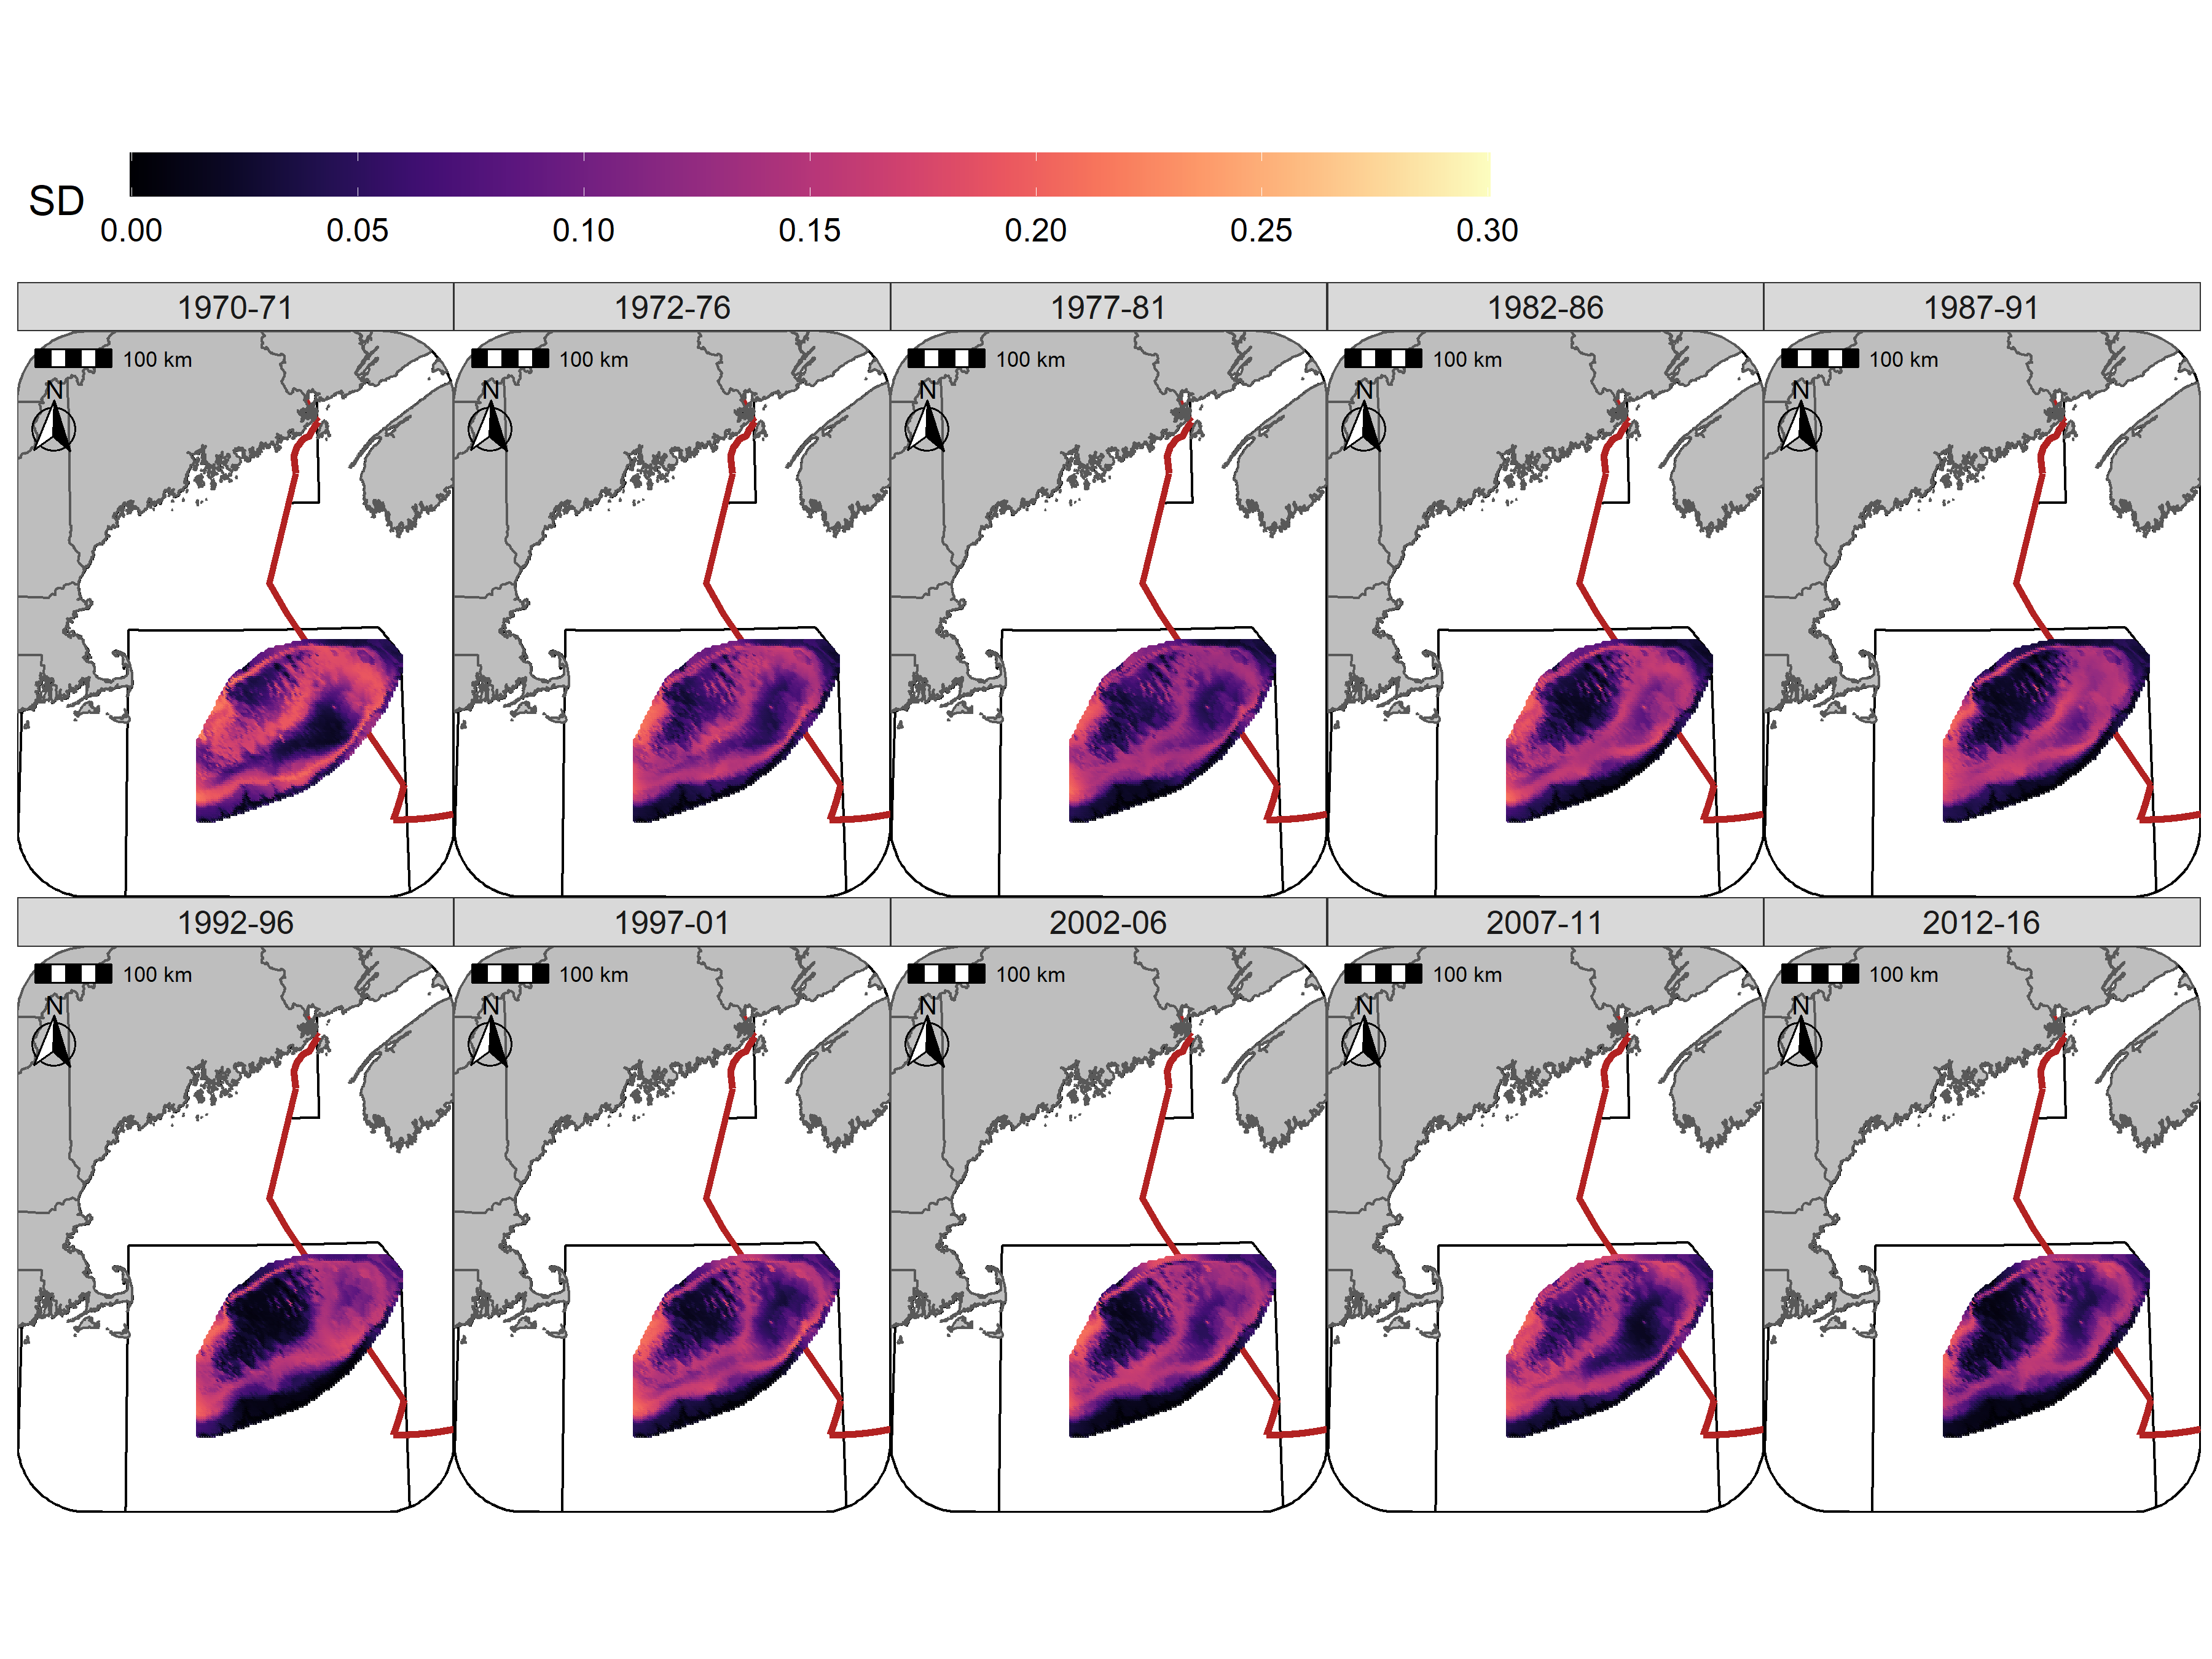
\includegraphics[width=1\linewidth]{D:/Github/Paper_2_SDMs/Results/Figures/pf_fall_yt_sd} \caption{Standard deviation (logit scale) of predicted occurrence probability for Yellowtail Flounder in each era during the Fall (NMFS-fall survey) using the SST + Dep + Sed  model and 5-year random field.}\label{fig:pf-fall-yt-sd}
\end{figure}
\end{landscape}

\clearpage

\hypertarget{random-fields}{%
\subsection{Random fields}\label{random-fields}}

The 5-year random fields for Atlantic Cod in the Winter and Spring are seasonally consistent through time, with lower effect sizes observed in both seasons starting in 1992 and the largest declines in the effect size observed in the southern and western portions of GB (Figures \ref{fig:rf-winter-cod} - \ref{fig:rf-spring-cod}). In the Fall the higher effect sizes were generally observed towards the north and in Canadian waters, with larger declines in the random field effect size towards the west over the study period (Figure \ref{fig:rf-fall-cod}).

The Yellowtail Flounder random field patterns were similar in the Winter and Spring while the random field effect sizes were somewhat smaller during the Fall (Figures \ref{fig:rf-winter-yt} - \ref{fig:rf-fall-yt}). The effect size of the random fields, in all seasons, were lower throughout the latter half of the 1980s and the early 1990s. The highest effect size of the random fields were observed in the 1970s and in the 2000s. Since the mid-1970s an area straddling the Canadian-U.S. border has been consistently identified as an area where the Yellowtail Flounder effect size of the random field is elevated (Figures \ref{fig:rf-winter-yt} - \ref{fig:rf-fall-yt}).

The standard deviation (SD) of the random fields for Atlantic Cod were also similar between seasons with the lowest SD generally observed in the north and east and highest approaching the southern flank of GB. The SD was somewhat higher in the Fall throughout the central portion of GB (Figures \ref{fig:rf-winter-cod-sd} - \ref{fig:rf-fall-cod-sd}). For Yellowtail Flounder, the SD was higher towards the southern portions of the bank with localized regions having elevated SD scattered throughout the bank in the Winter, Spring, and Fall. (Figures \ref{fig:rf-winter-yt-sd} - \ref{fig:rf-fall-yt-sd}).

\begin{landscape}
\begin{figure}
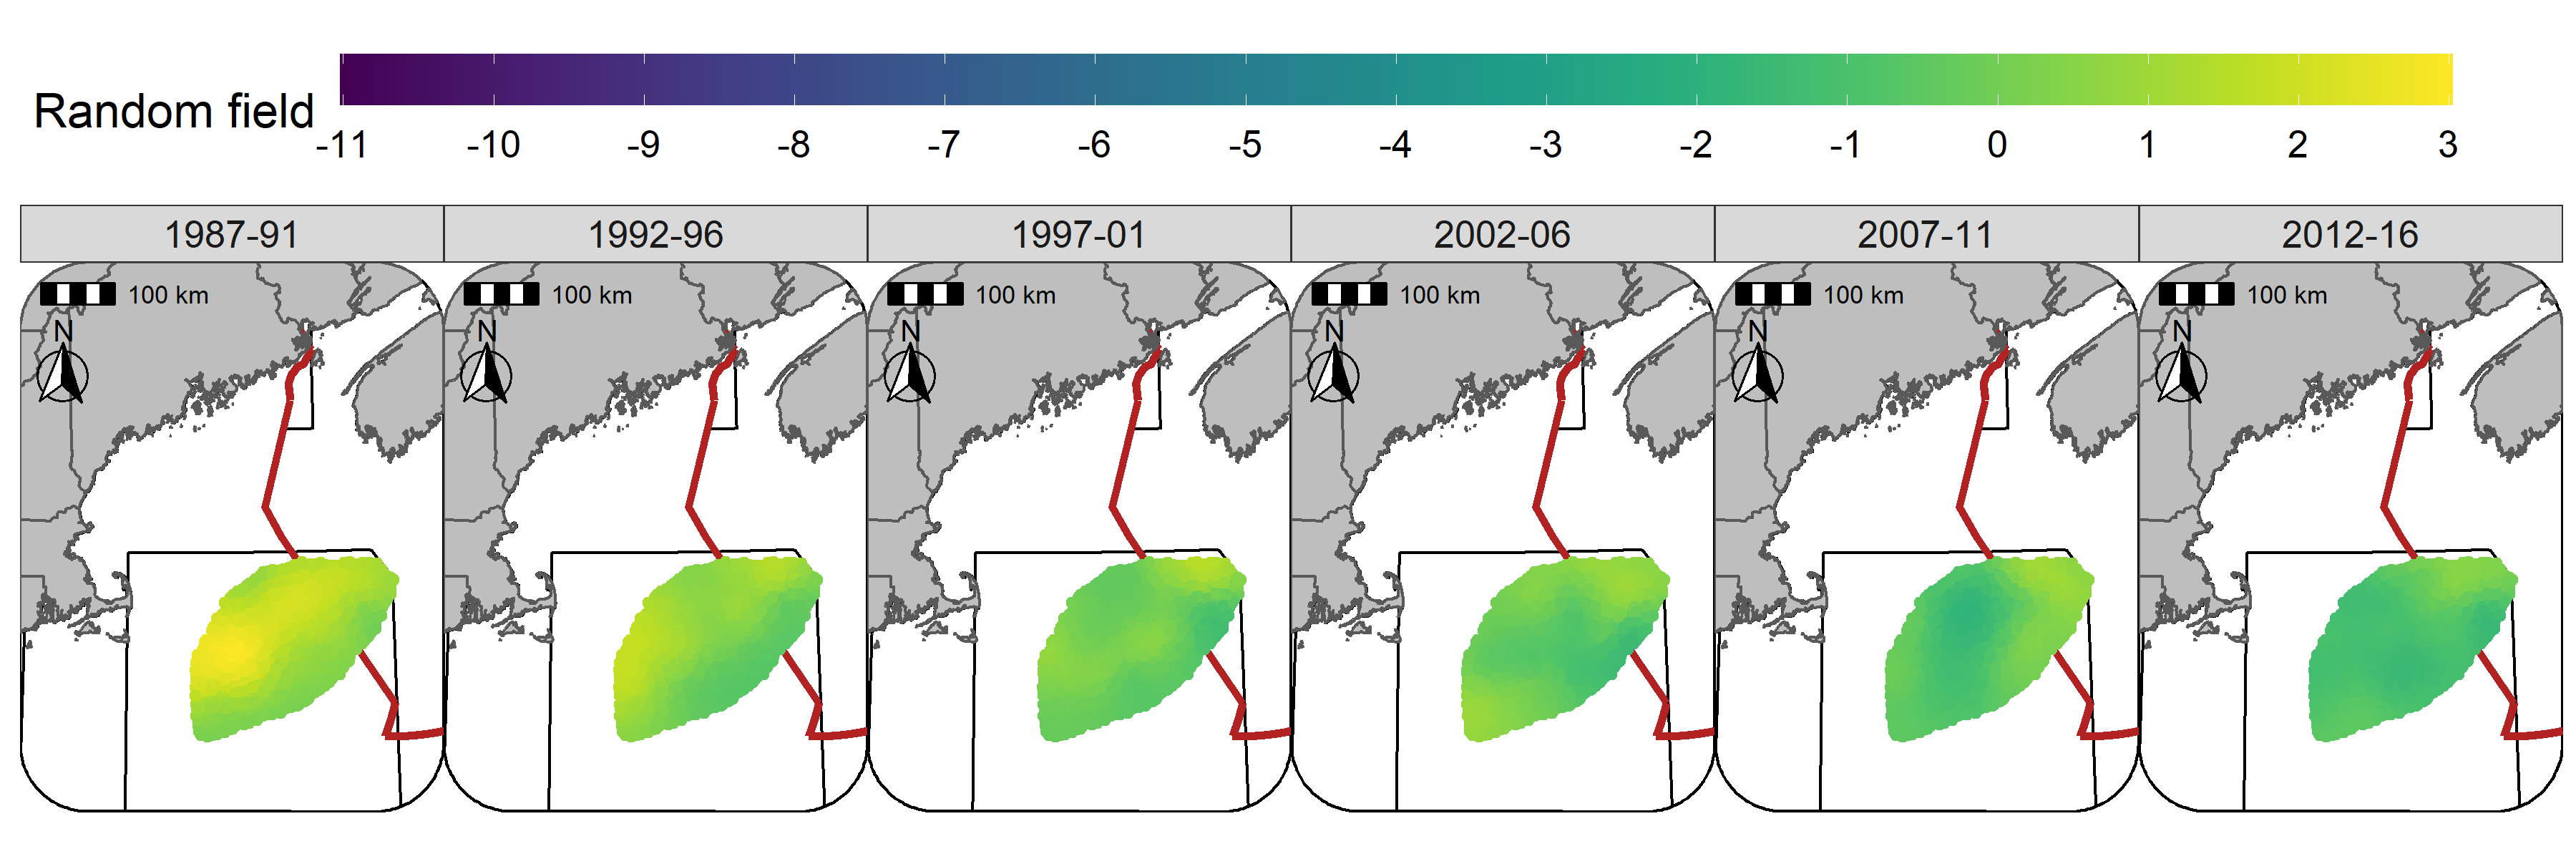
\includegraphics[width=1\linewidth]{D:/Github/Paper_2_SDMs/Results/Figures/rf_winter_cod} \caption{Random fields (logit scale) for Atlantic Cod  in each era during the Winter (RV survey) using the SST + Dep model and 5-year random field.}\label{fig:rf-winter-cod}
\end{figure}

\newpage
\begin{figure}
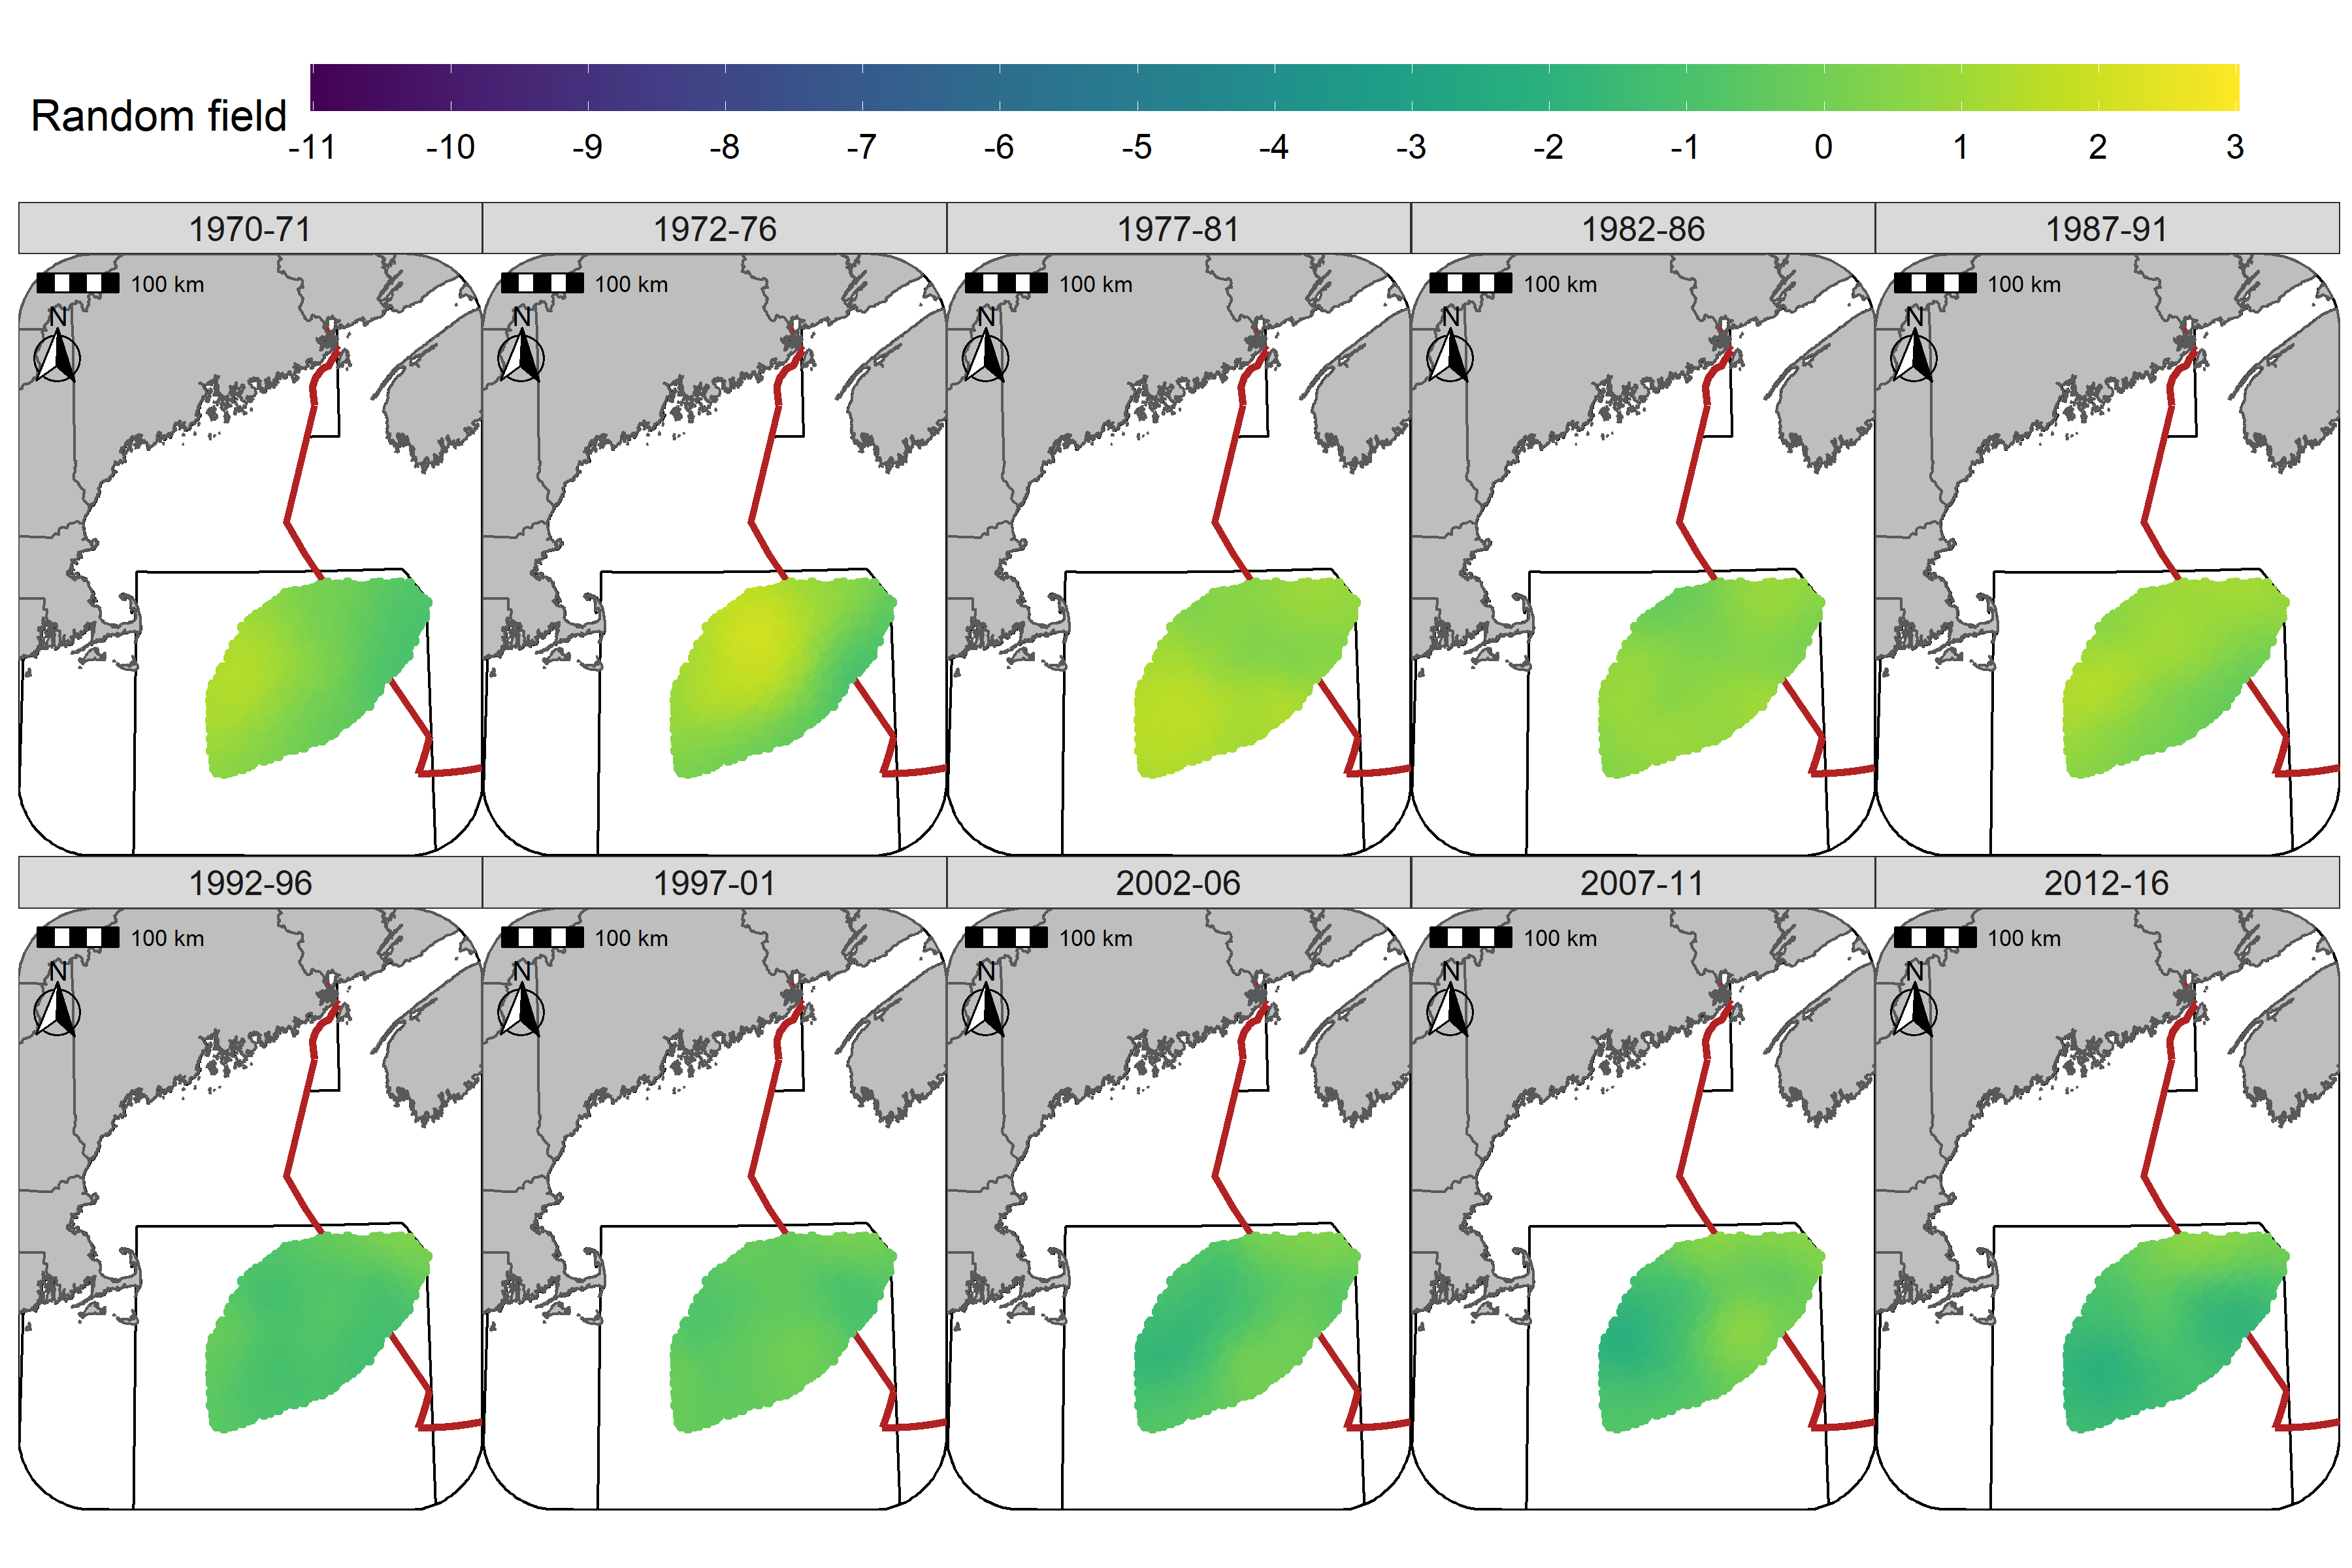
\includegraphics[width=1\linewidth]{D:/Github/Paper_2_SDMs/Results/Figures/rf_spring_cod} \caption{Random fields (logit scale) for Atlantic Cod  in each era during the Spring (NMFS-spring survey) using the SST + Dep model and 5-year random field.}\label{fig:rf-spring-cod}
\end{figure}

\newpage
\begin{figure}
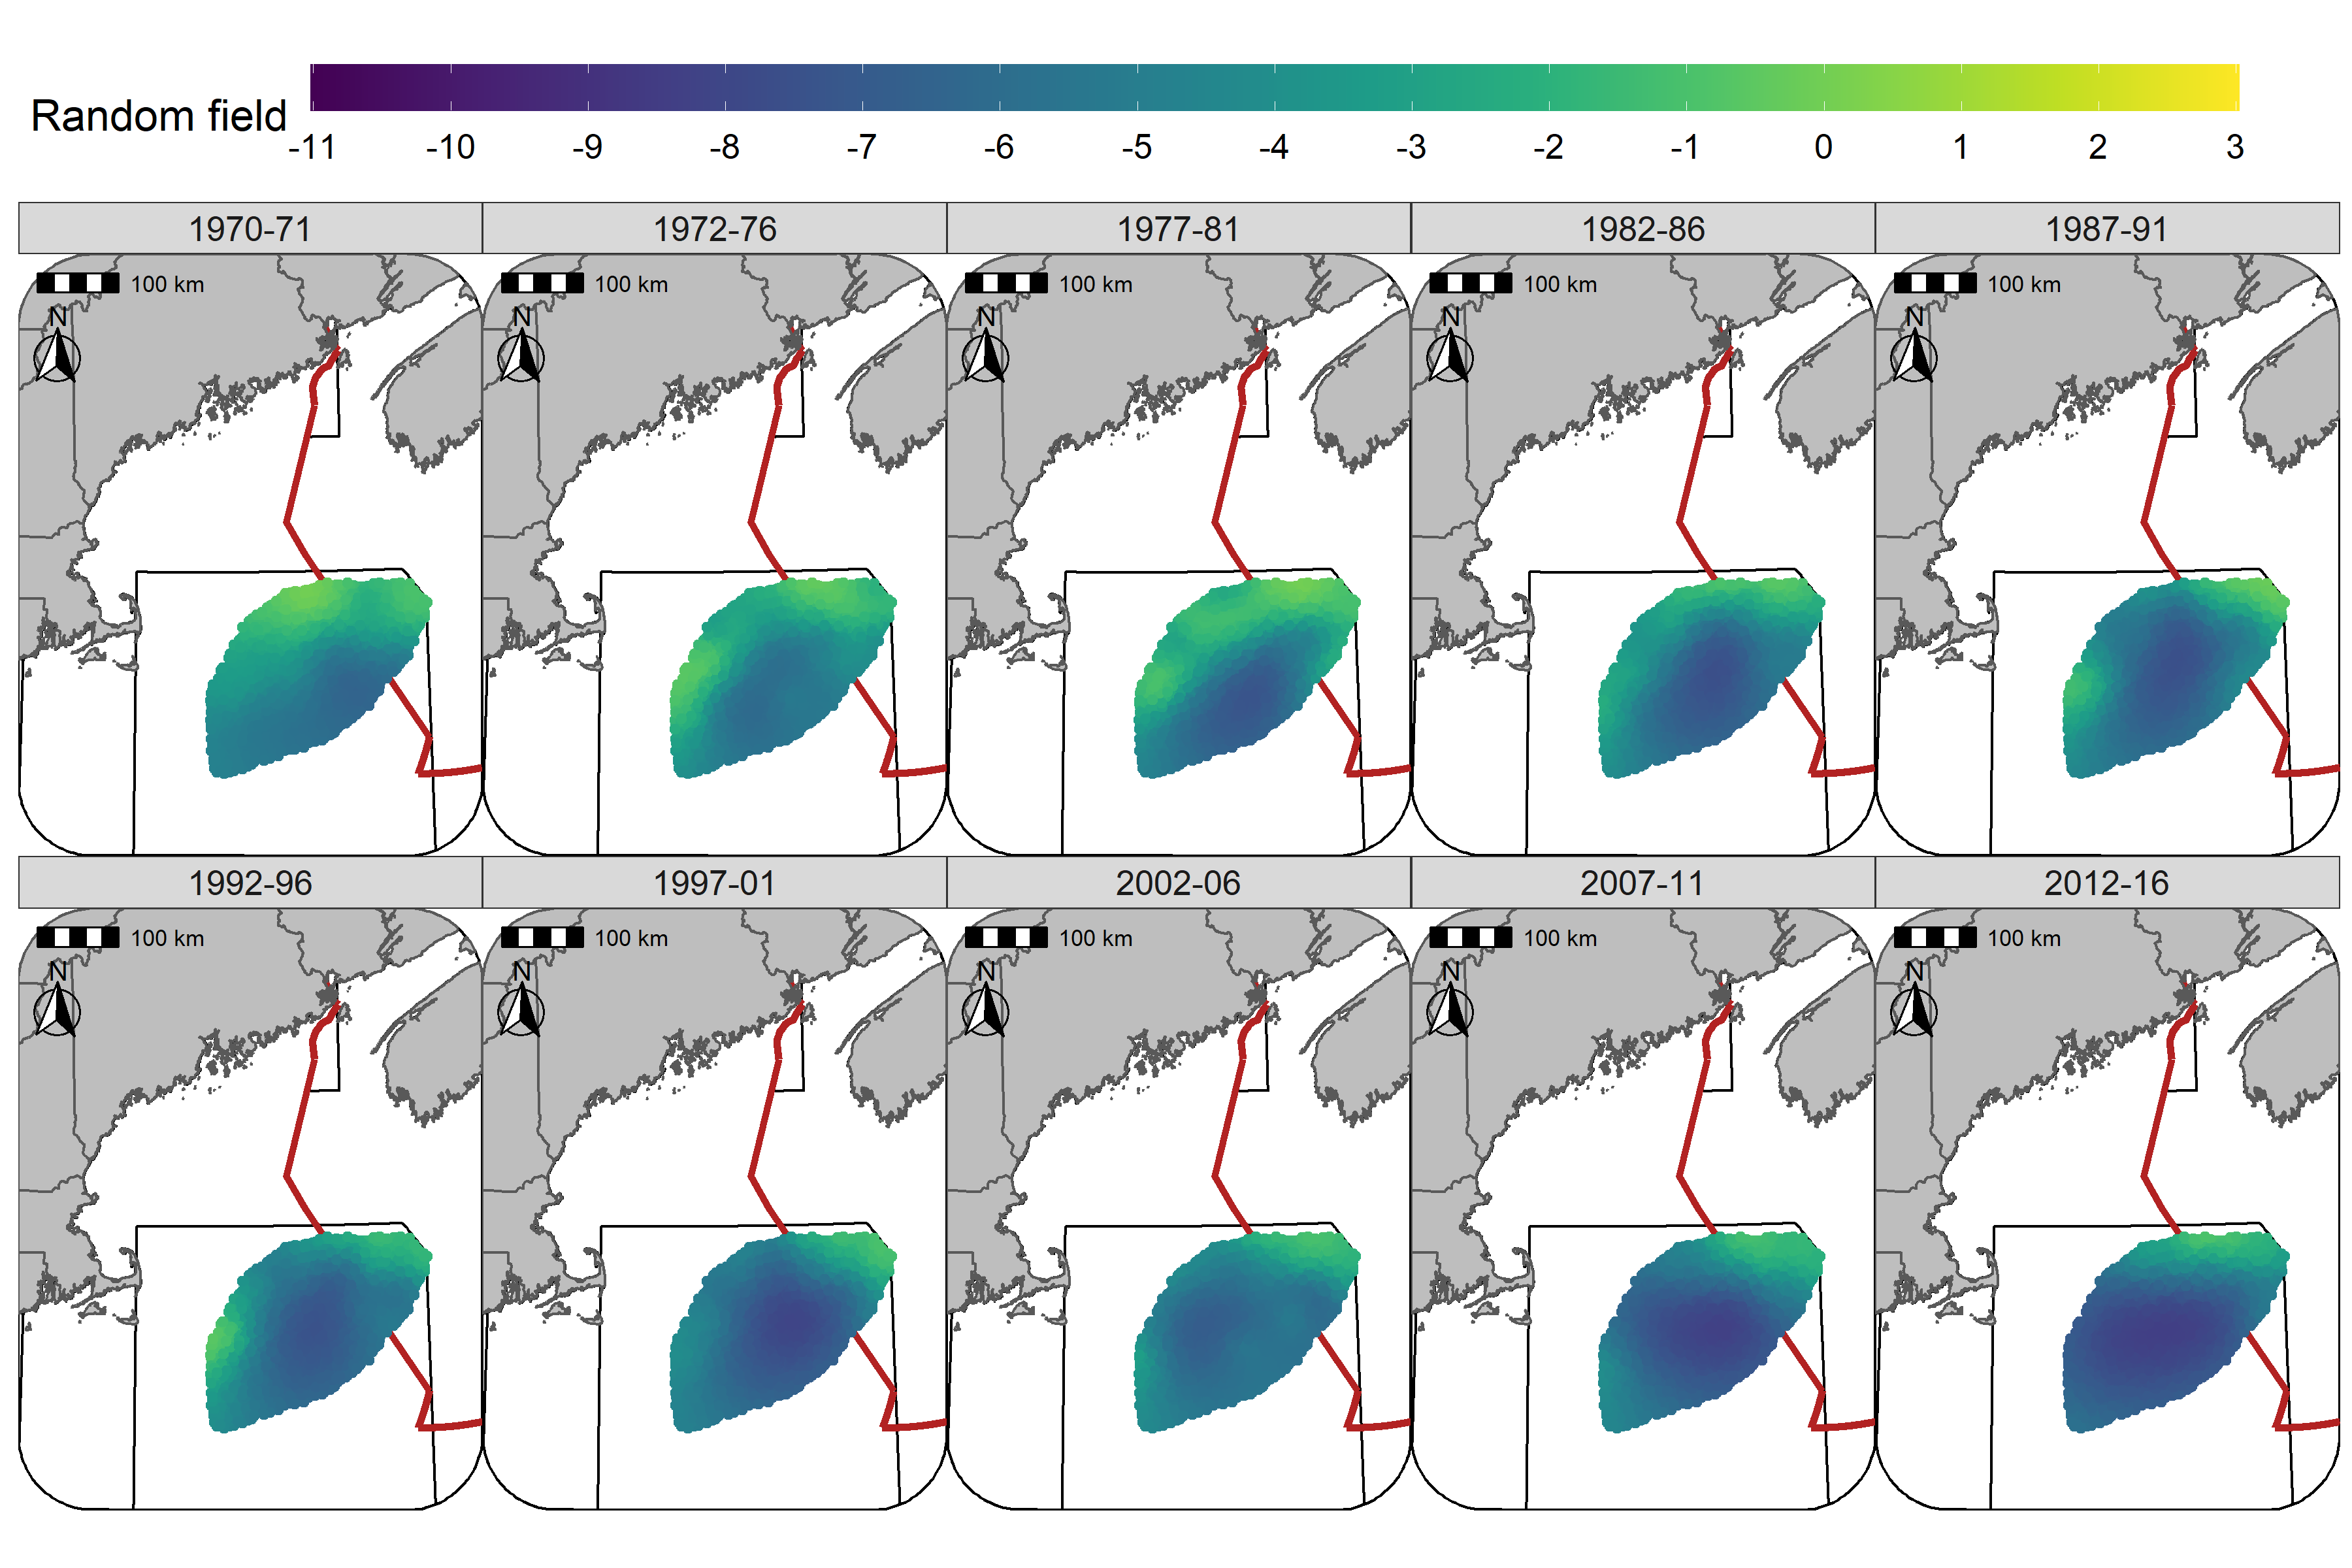
\includegraphics[width=1\linewidth]{D:/Github/Paper_2_SDMs/Results/Figures/rf_fall_cod} \caption{Random fields (logit scale) for Atlantic Cod  in each era during the Fall (NMFS-fall survey) using the SST + Dep model and 5-year random field.}\label{fig:rf-fall-cod}
\end{figure}

\newpage
\begin{figure}
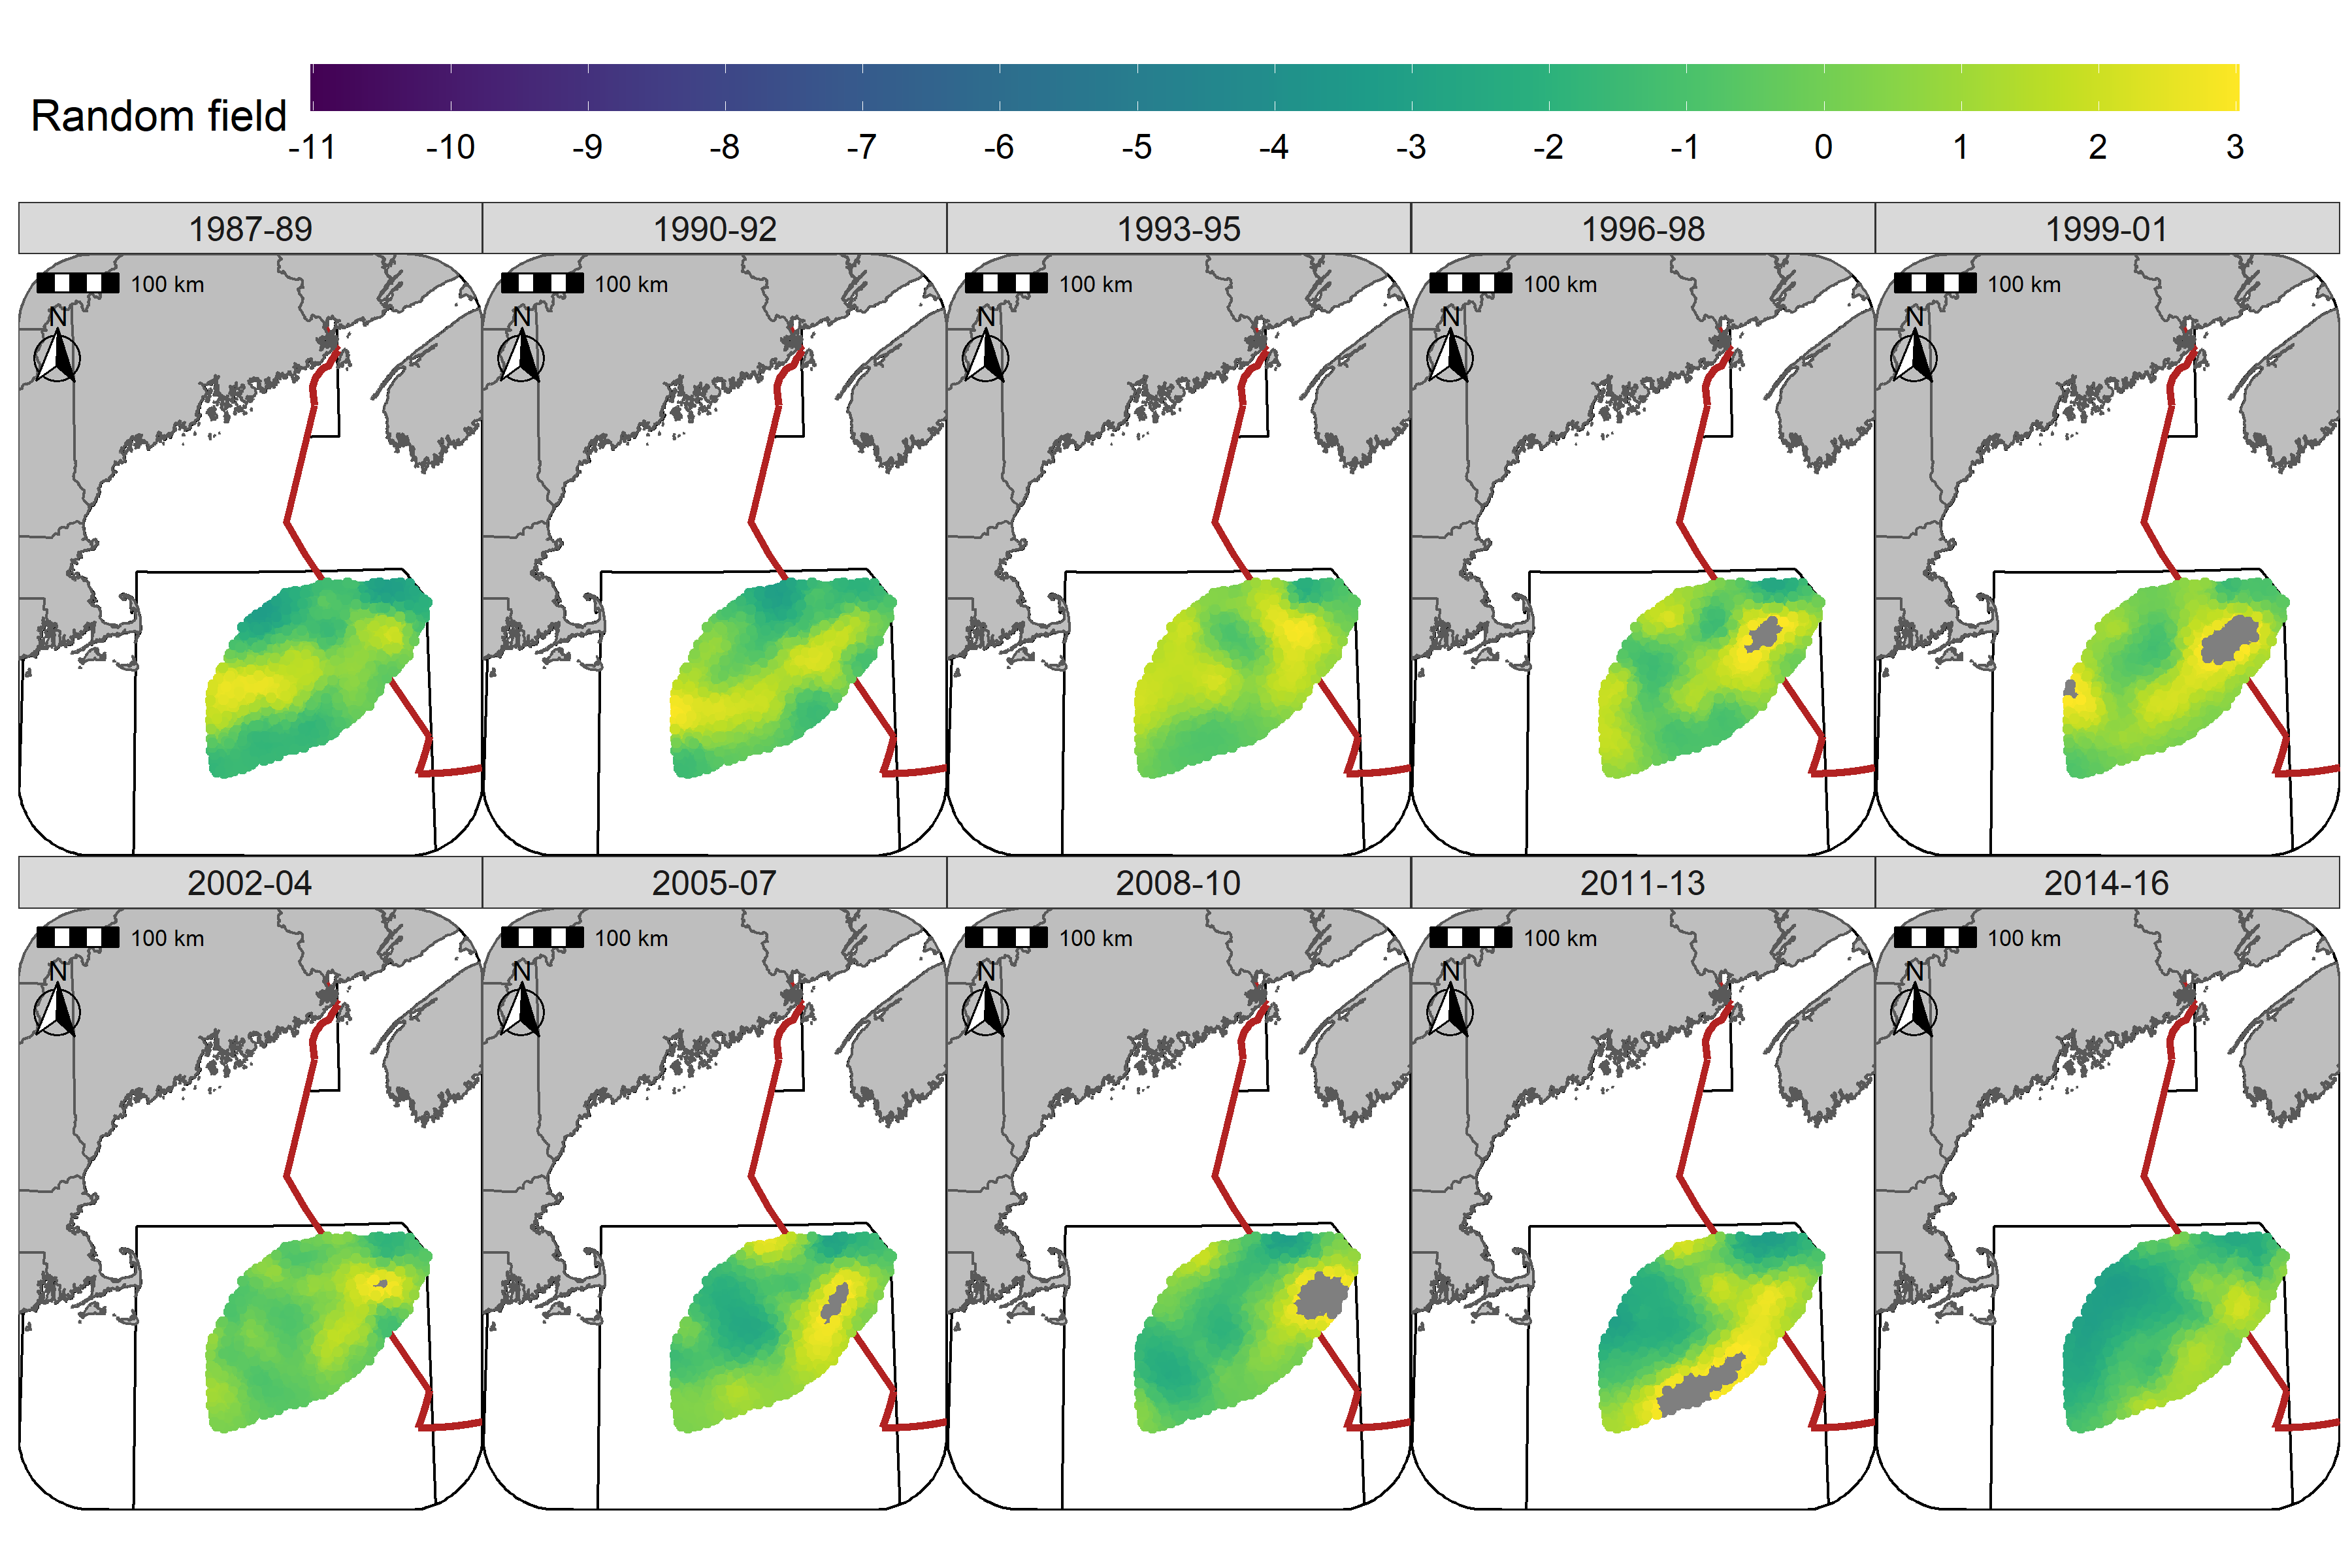
\includegraphics[width=1\linewidth]{D:/Github/Paper_2_SDMs/Results/Figures/rf_winter_yt} \caption{Random fields (logit scale) for Yellowtail Flounder in each era during the Winter (RV survey) using the SST + Dep + Sed model and 3-year random field.}\label{fig:rf-winter-yt}
\end{figure}

\newpage
\begin{figure}
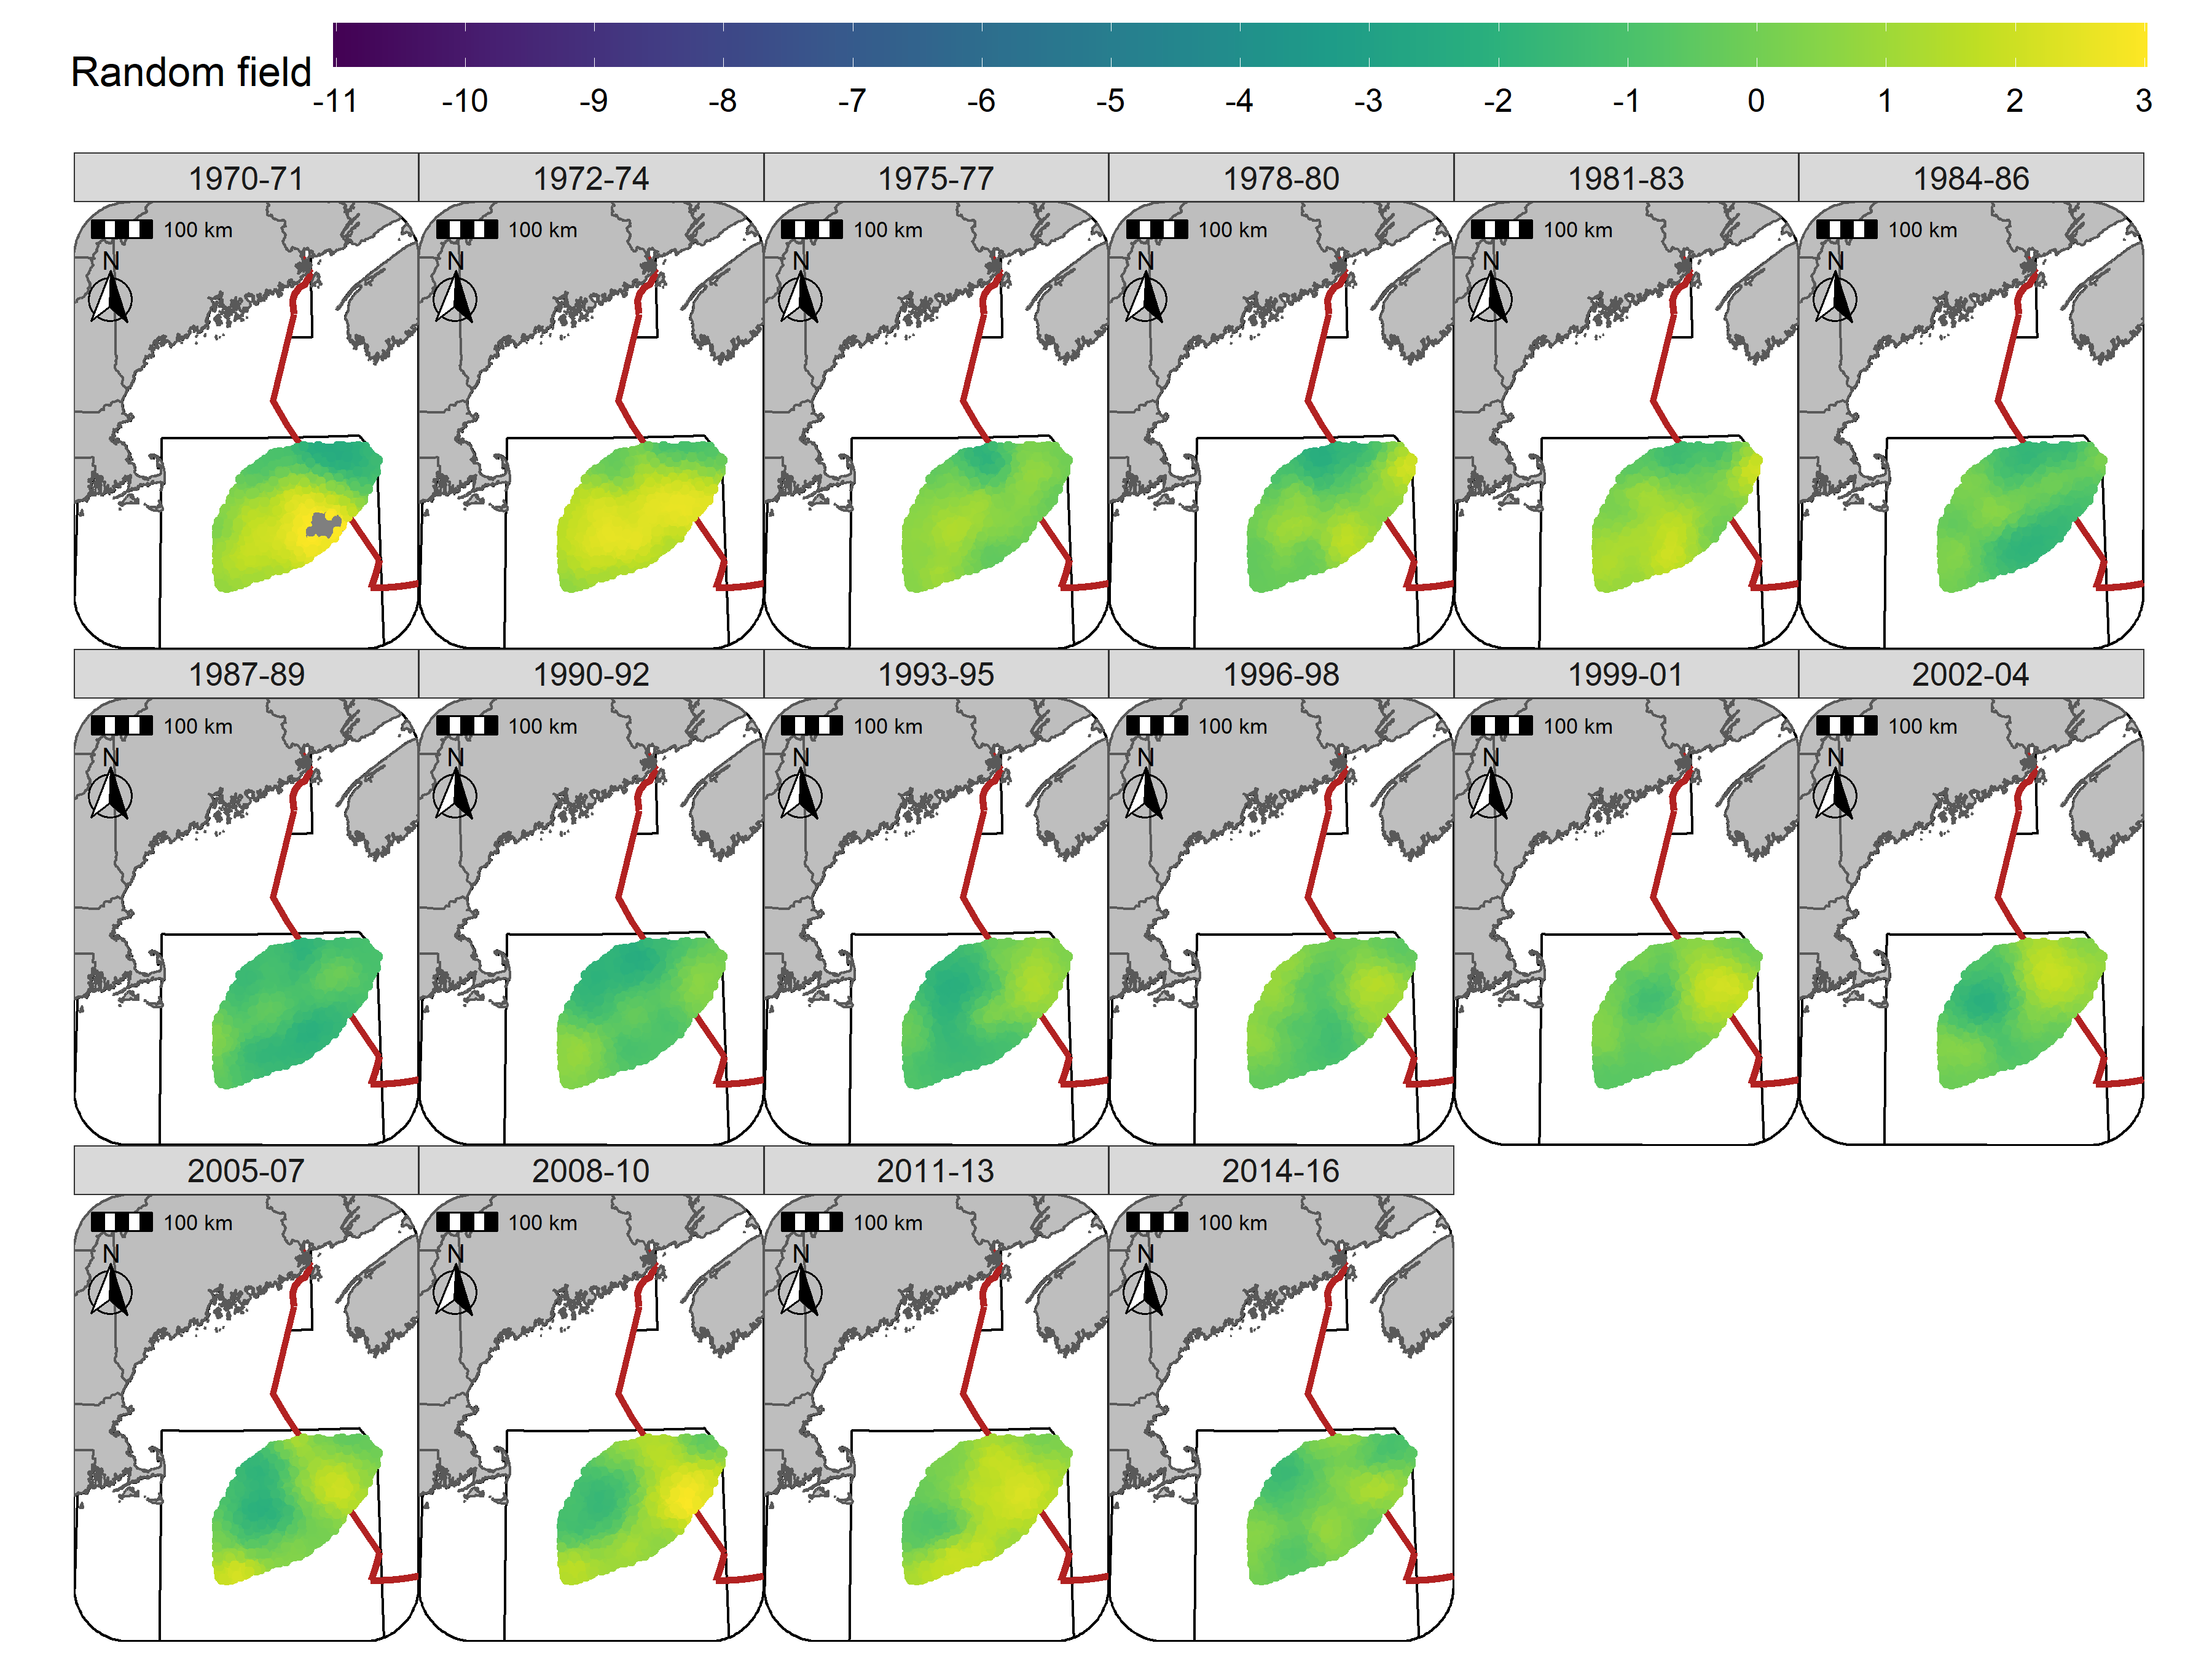
\includegraphics[width=1\linewidth]{D:/Github/Paper_2_SDMs/Results/Figures/rf_spring_yt} \caption{Random fields (logit scale) for Yellowtail Flounder in each era during the Spring (NMFS-spring survey) using the SST + Dep + Sed model and 3-year random field.}\label{fig:rf-spring-yt}
\end{figure}

\newpage
\begin{figure}
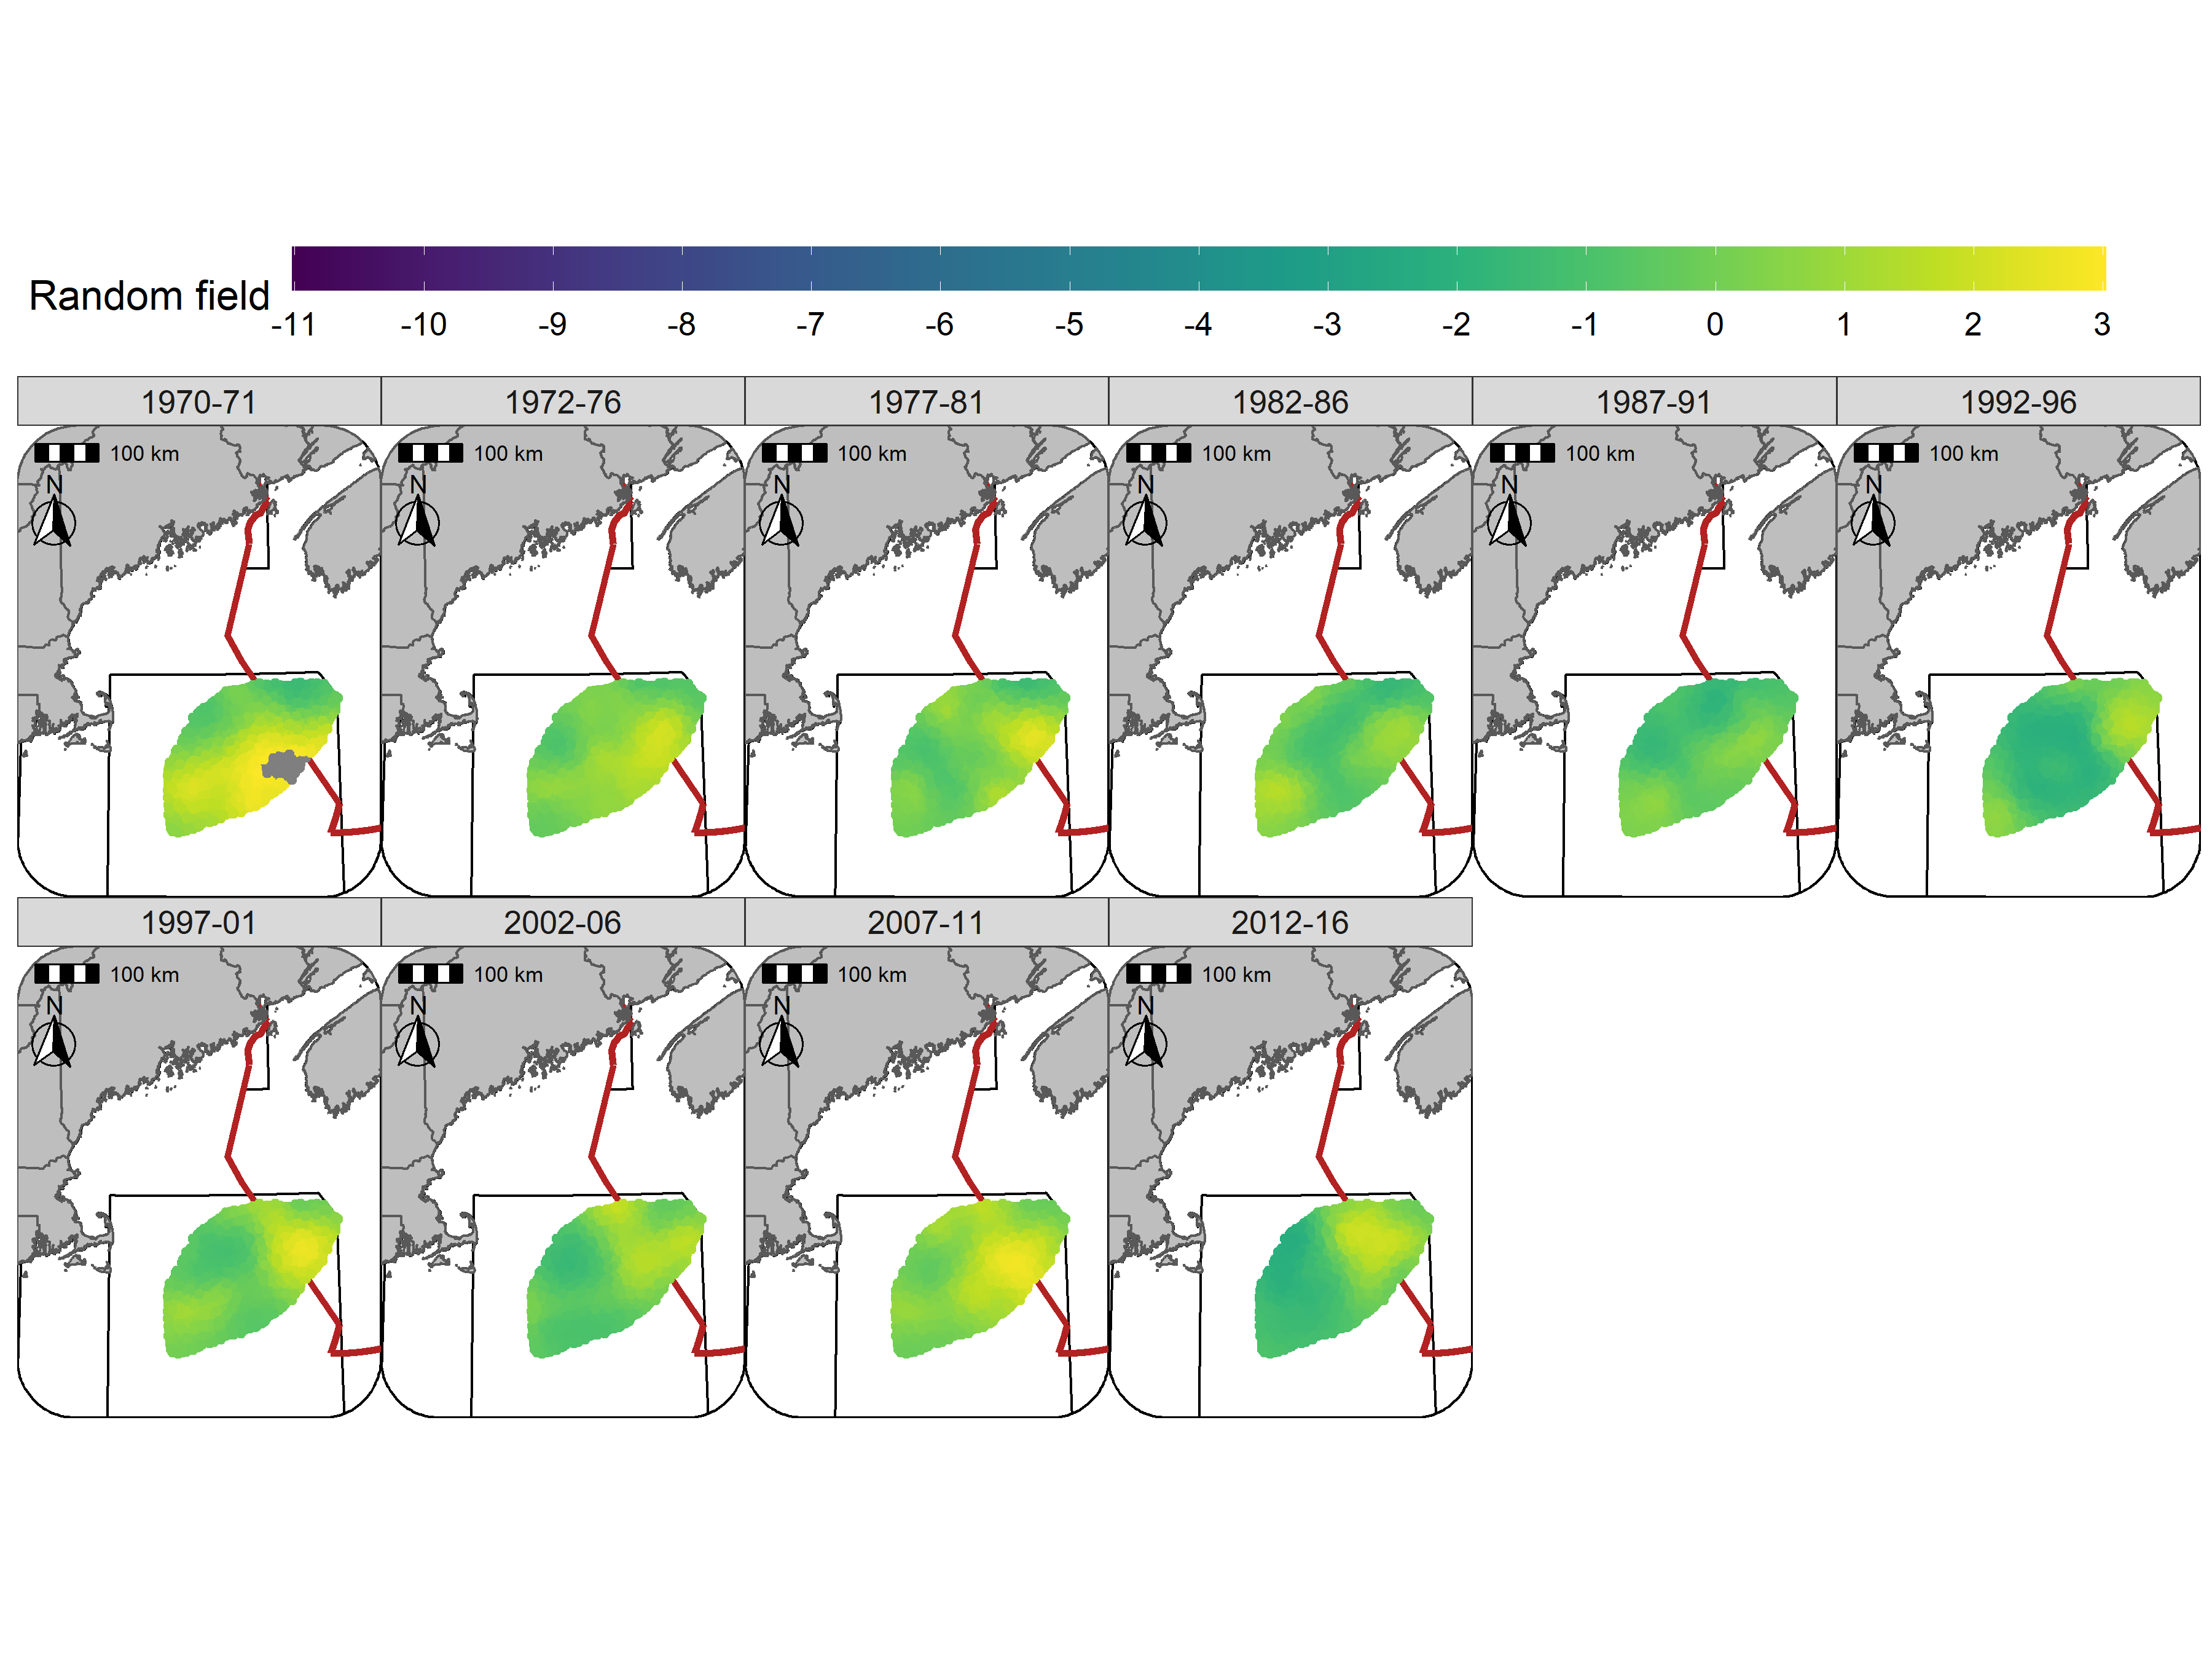
\includegraphics[width=1\linewidth]{D:/Github/Paper_2_SDMs/Results/Figures/rf_fall_yt} \caption{Random fields (logit scale) for Yellowtail Flounder in each era during the Fall (NMFS-fall survey) using the SST + Dep + Sed model and 5-year random field.}\label{fig:rf-fall-yt}
\end{figure}

\newpage

\begin{figure}
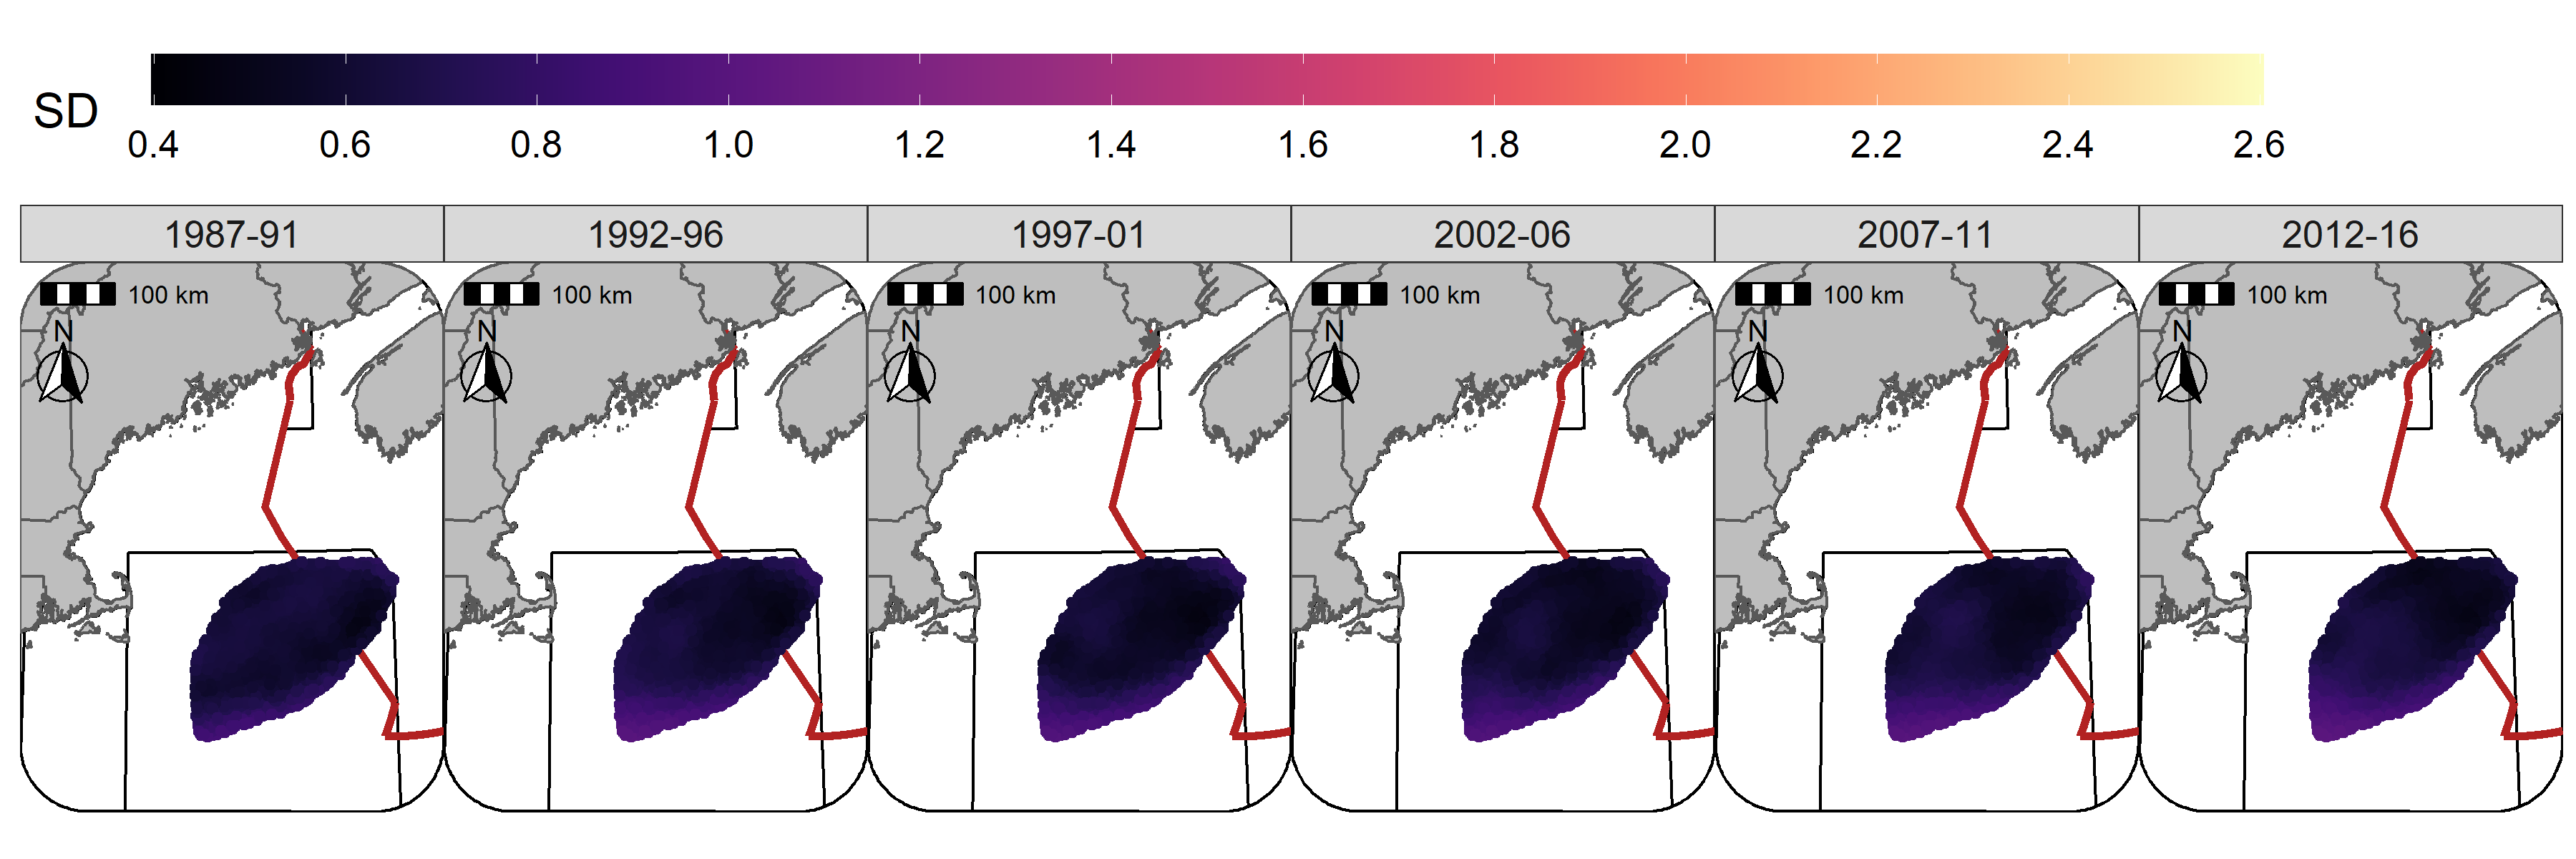
\includegraphics[width=1\linewidth]{D:/Github/Paper_2_SDMs/Results/Figures/rf_winter_cod_sd} \caption{Standard deviation of random fields (logit scale) for Atlantic Cod  in each era during the Winter (RV survey) using the SST + Dep model and 5-year random field.}\label{fig:rf-winter-cod-sd}
\end{figure}

\newpage
\begin{figure}
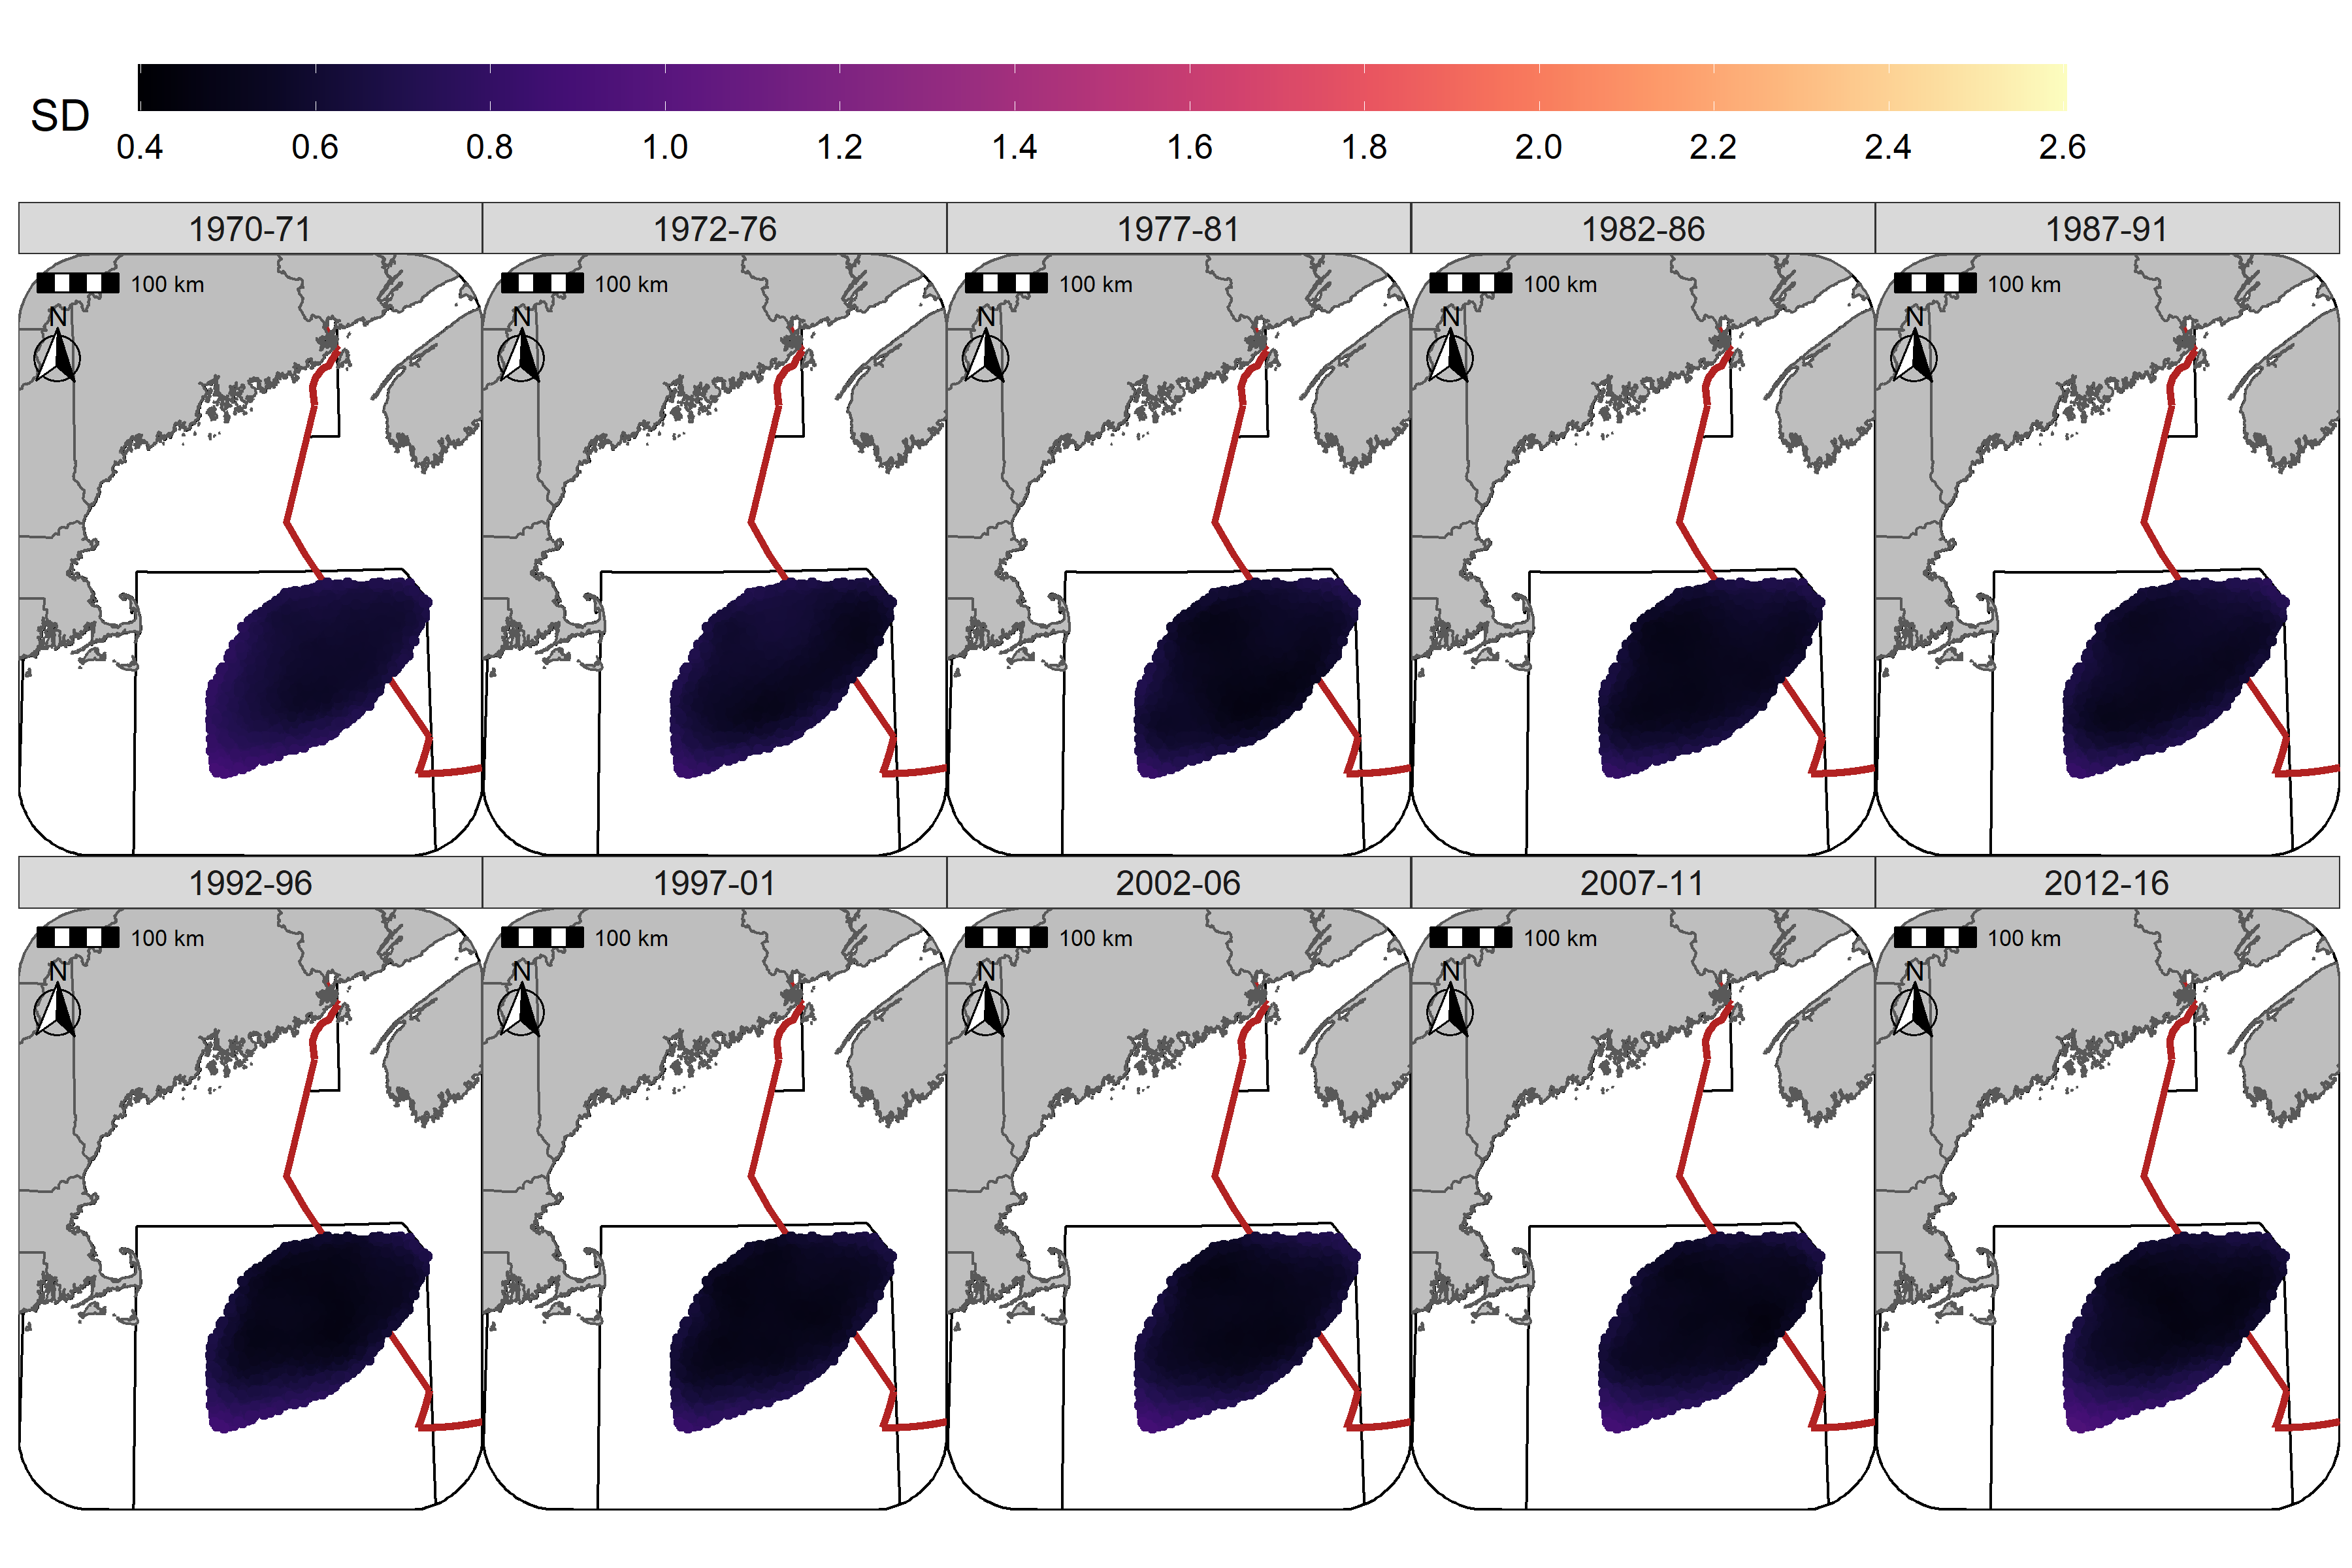
\includegraphics[width=1\linewidth]{D:/Github/Paper_2_SDMs/Results/Figures/rf_spring_cod_sd} \caption{Standard deviation of random fields (logit scale) for Atlantic Cod  in each era during the Spring (NMFS-spring survey) using the SST + Dep model and 5-year random field.}\label{fig:rf-spring-cod-sd}
\end{figure}

\newpage
\begin{figure}
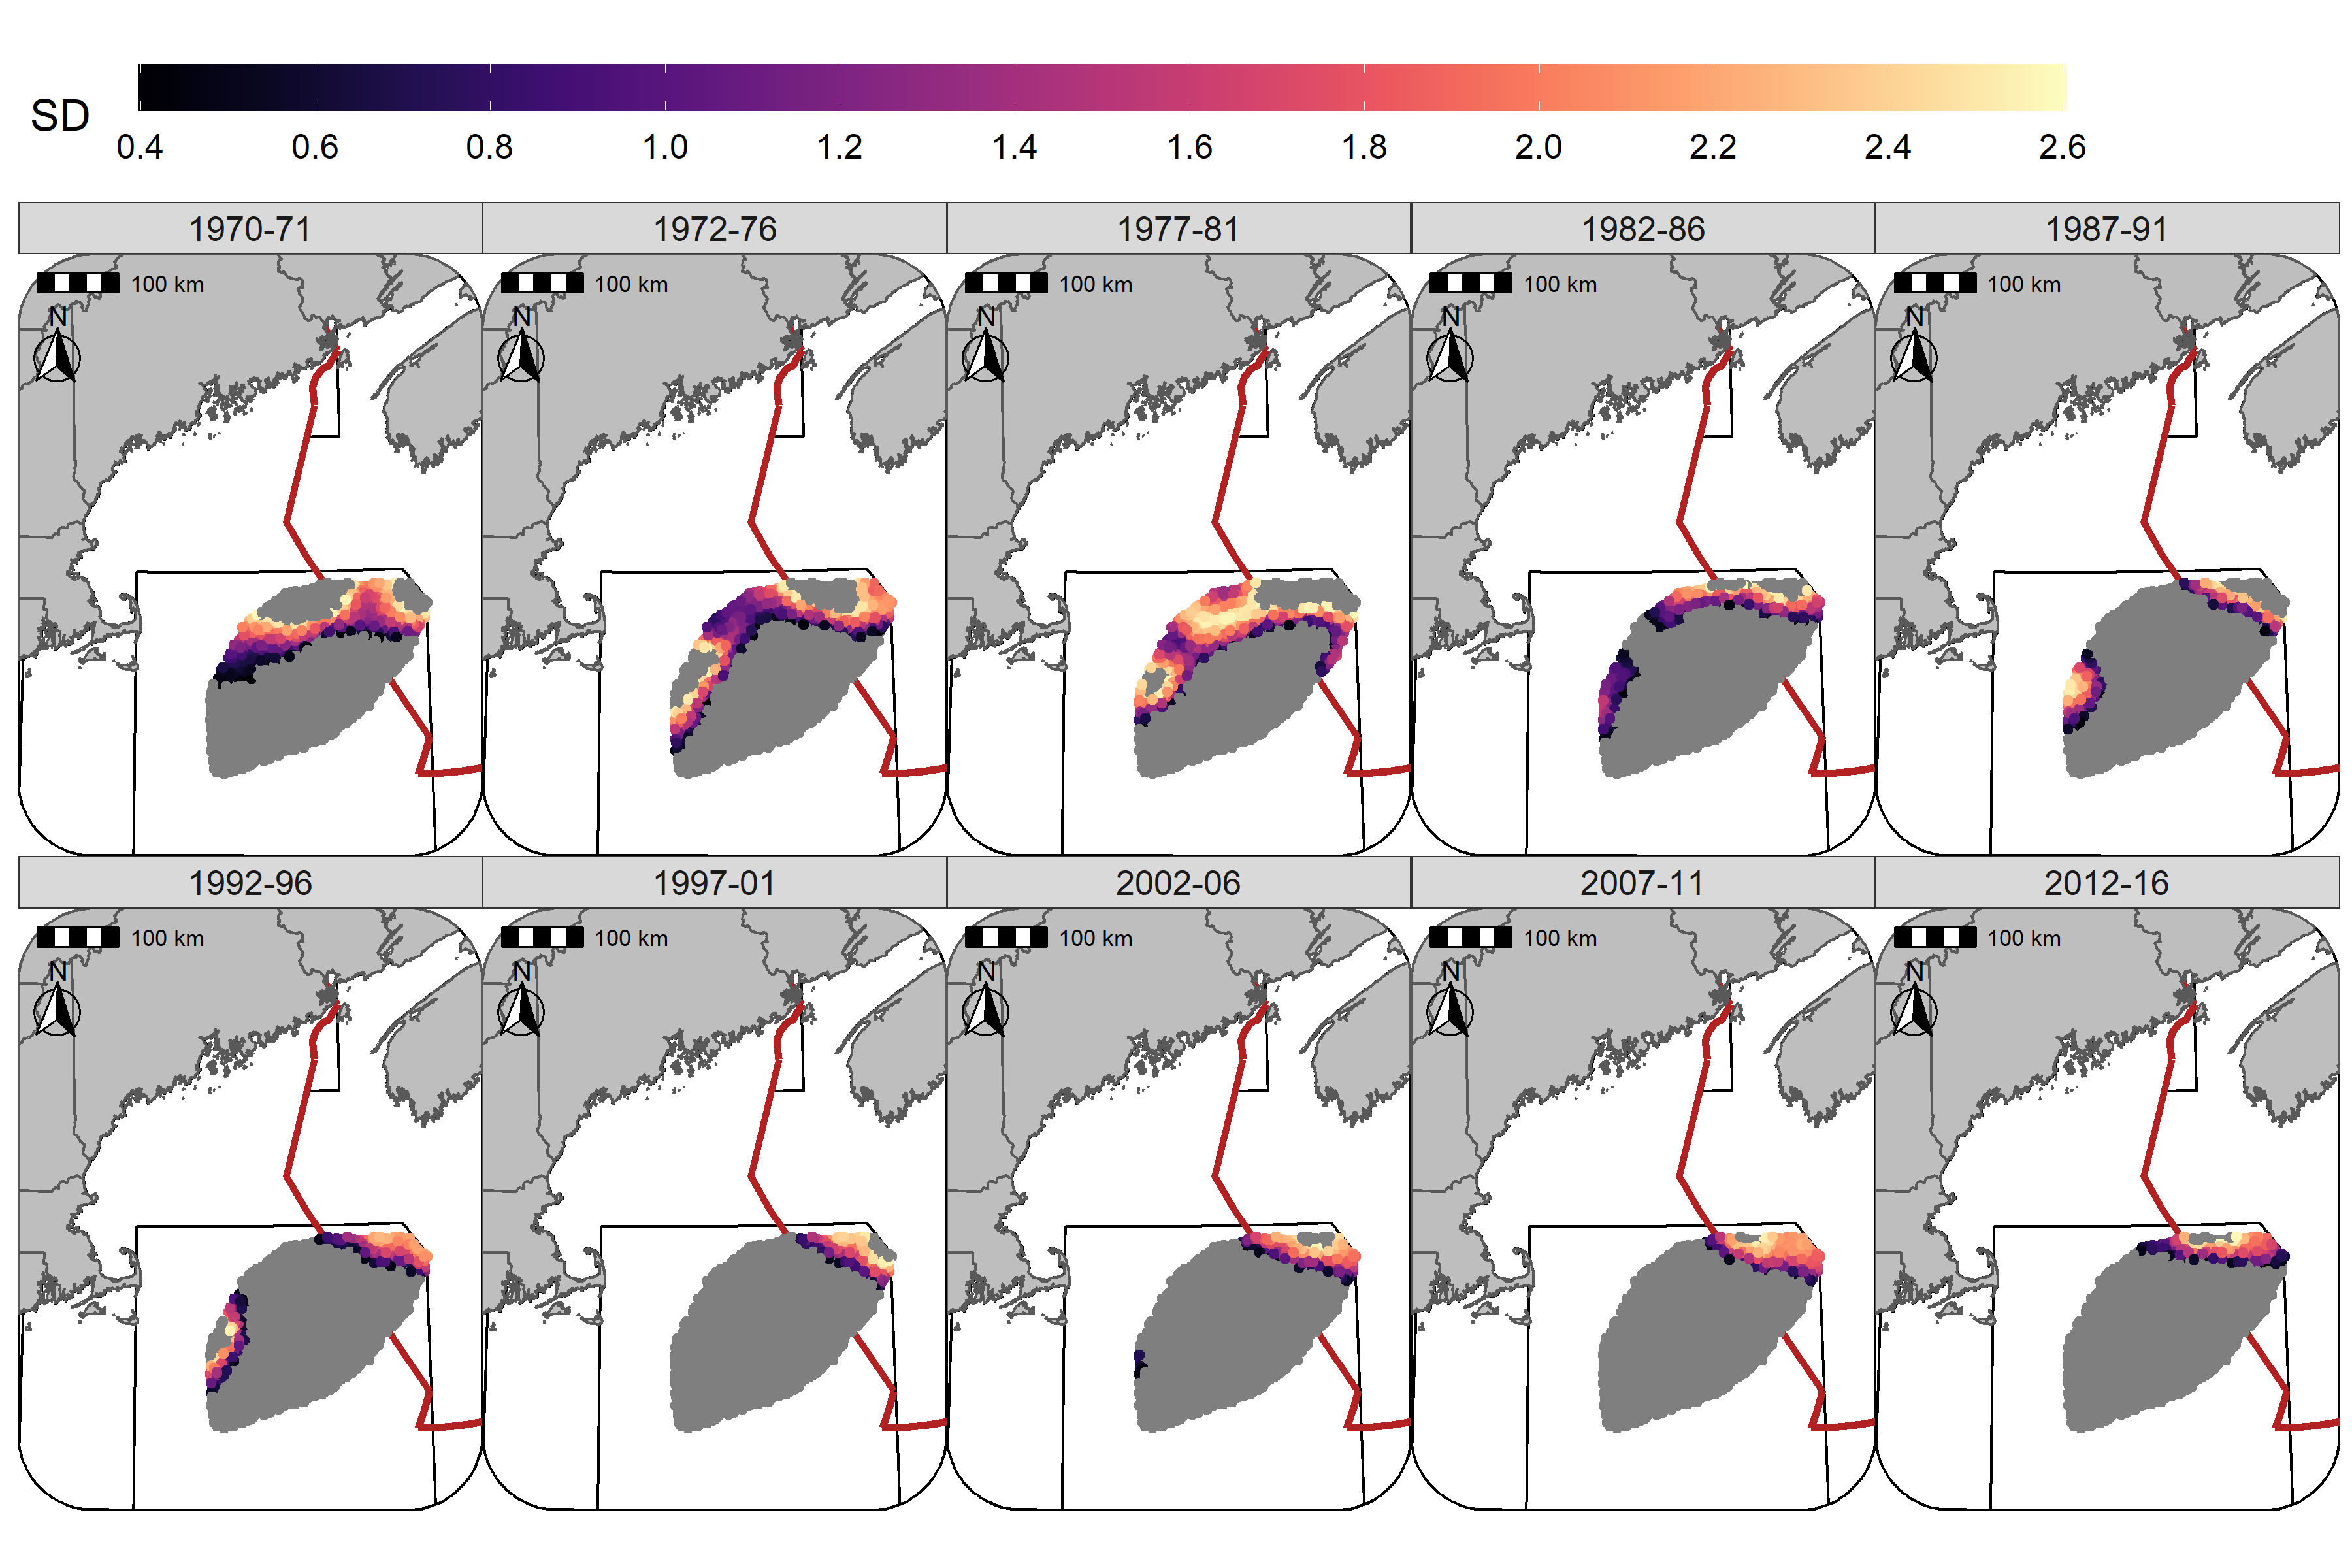
\includegraphics[width=1\linewidth]{D:/Github/Paper_2_SDMs/Results/Figures/rf_fall_cod_sd} \caption{Standard deviation of random fields (logit scale) for Atlantic Cod  in each era during the Fall (NMFS-fall survey) using the SST + Dep model and 5-year random field.}\label{fig:rf-fall-cod-sd}
\end{figure}

\newpage
\begin{figure}
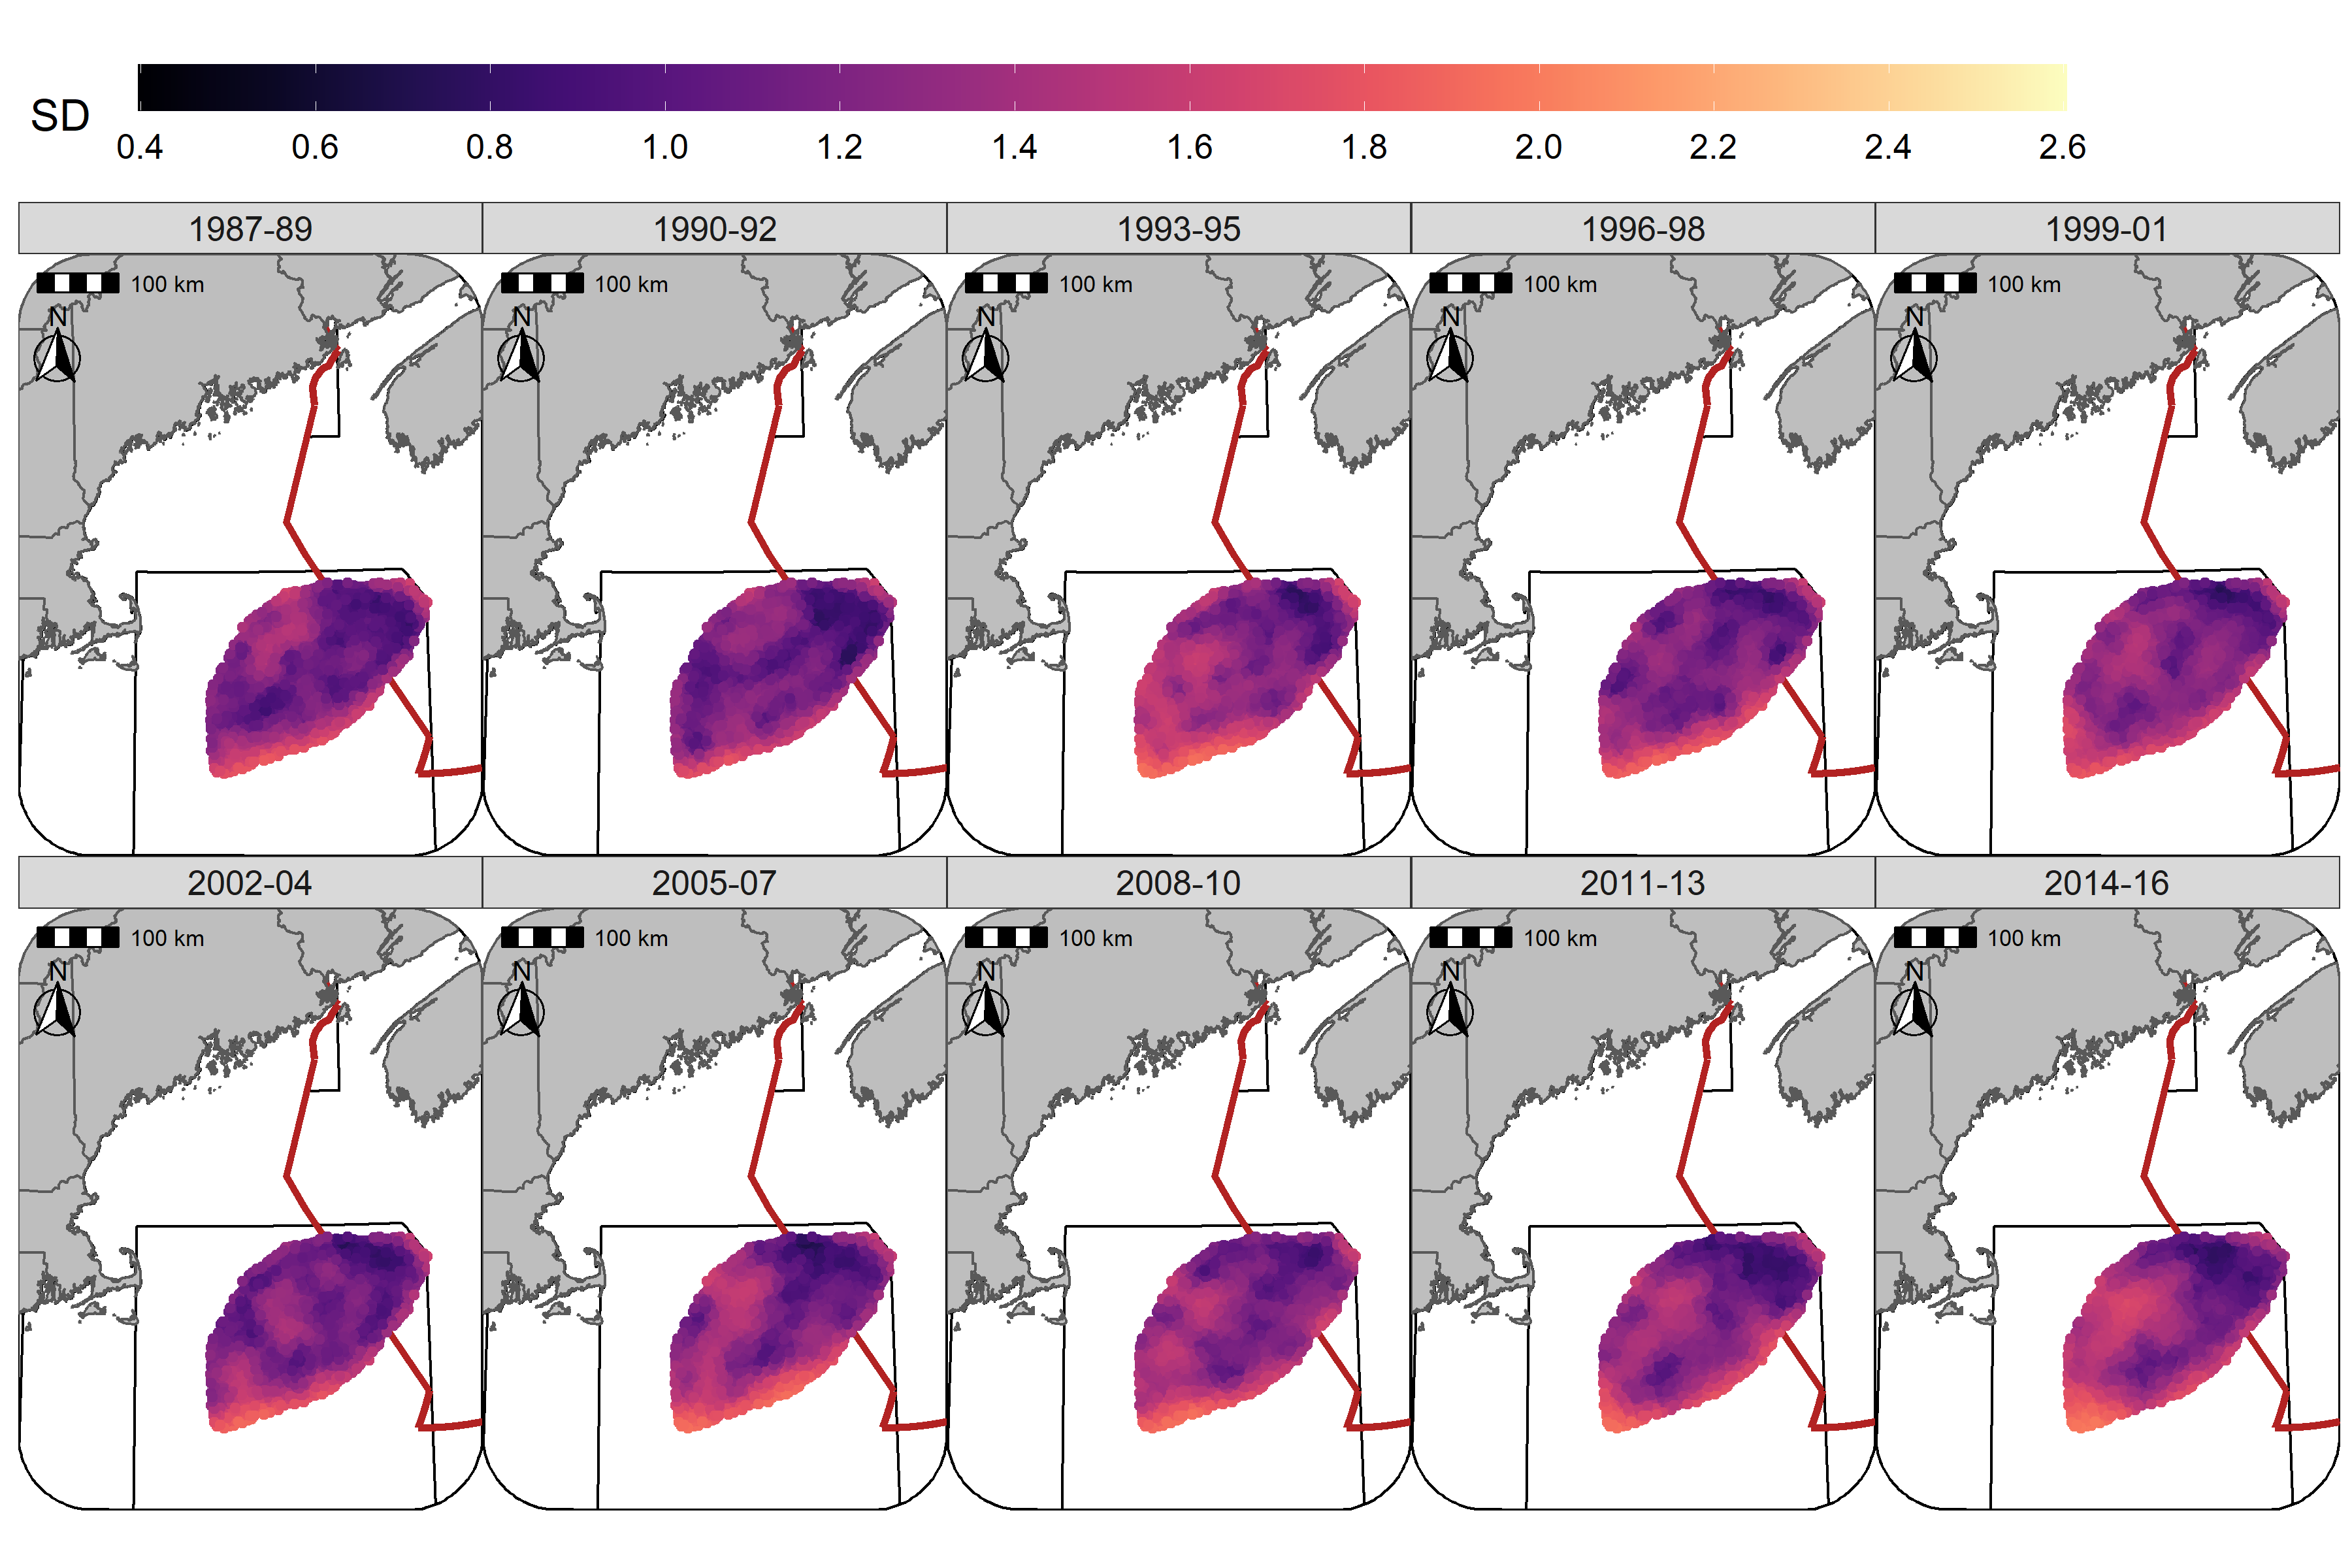
\includegraphics[width=1\linewidth]{D:/Github/Paper_2_SDMs/Results/Figures/rf_winter_yt_sd} \caption{Standard deviation of random fields (logit scale) for Yellowtail Flounder in each era during the Winter (RV survey) using the SST + Dep + Sed model and 3-year random field.}\label{fig:rf-winter-yt-sd}
\end{figure}

\newpage
\begin{figure}
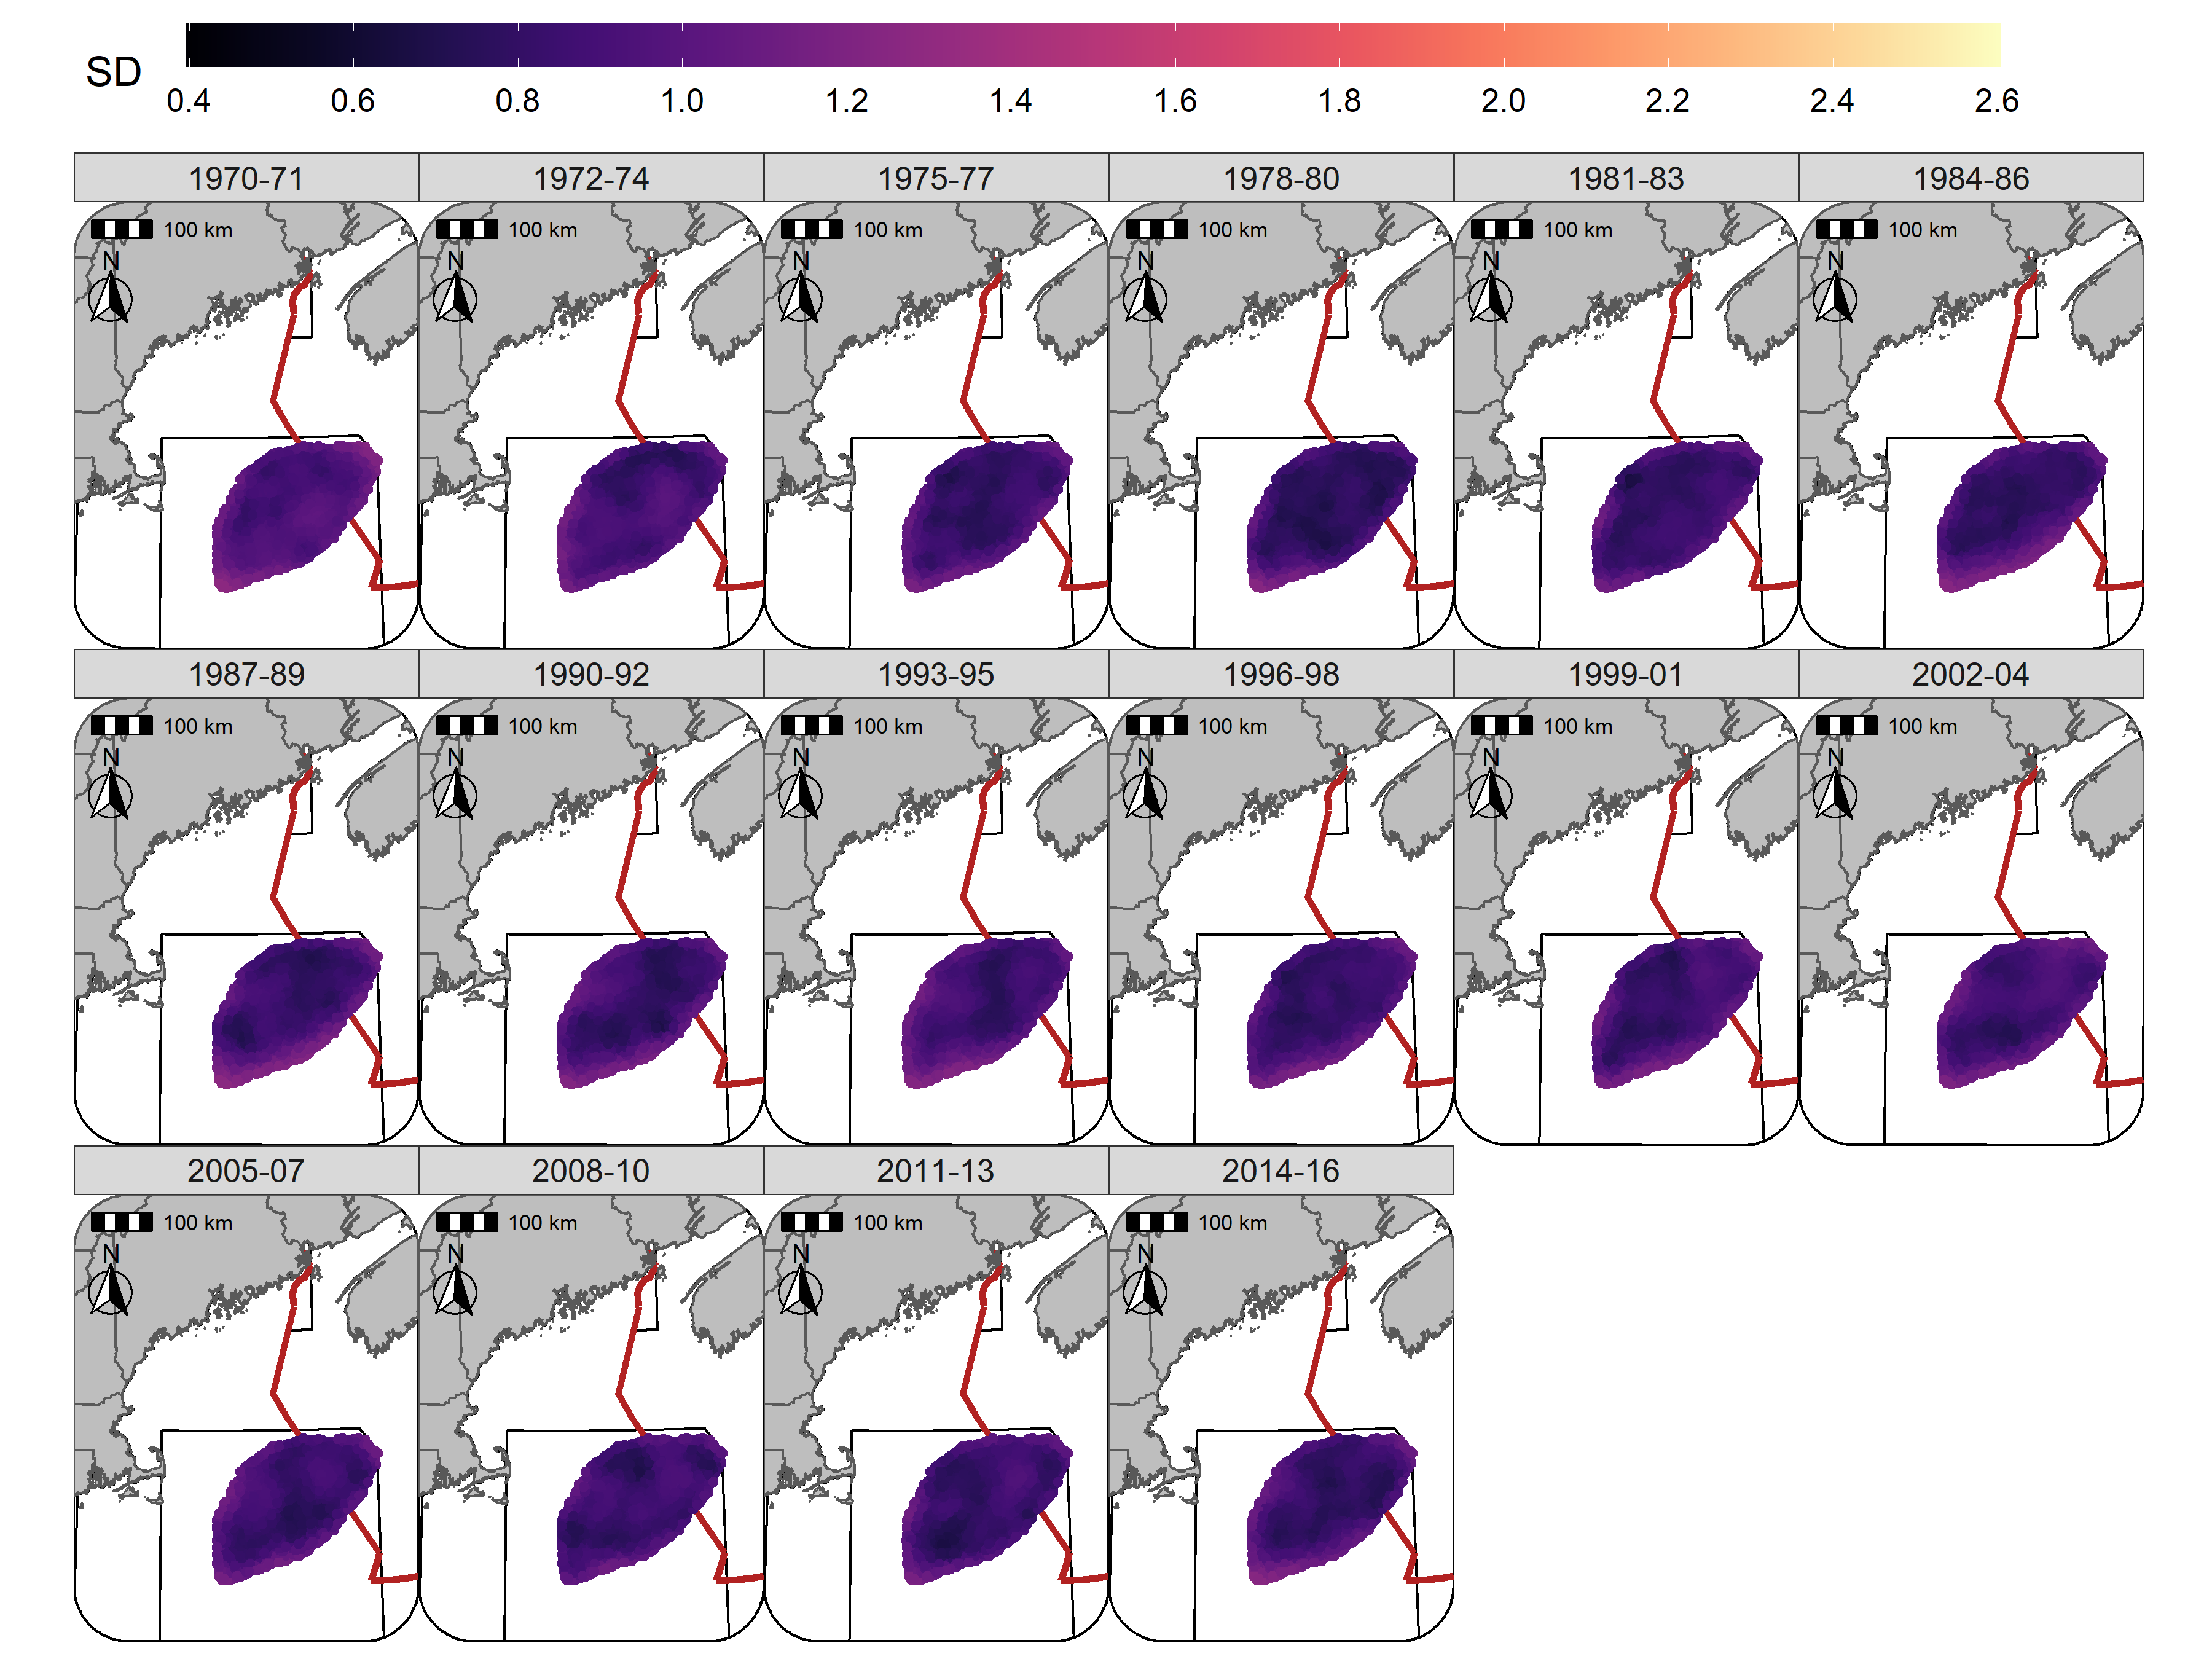
\includegraphics[width=1\linewidth]{D:/Github/Paper_2_SDMs/Results/Figures/rf_spring_yt_sd} \caption{Standard deviation of random fields (logit scale) for Yellowtail Flounder in each era during the Spring (NMFS-spring survey) using the SST + Dep + Sed model and 3-year random field.}\label{fig:rf-spring-yt-sd}
\end{figure}

\newpage
\begin{figure}
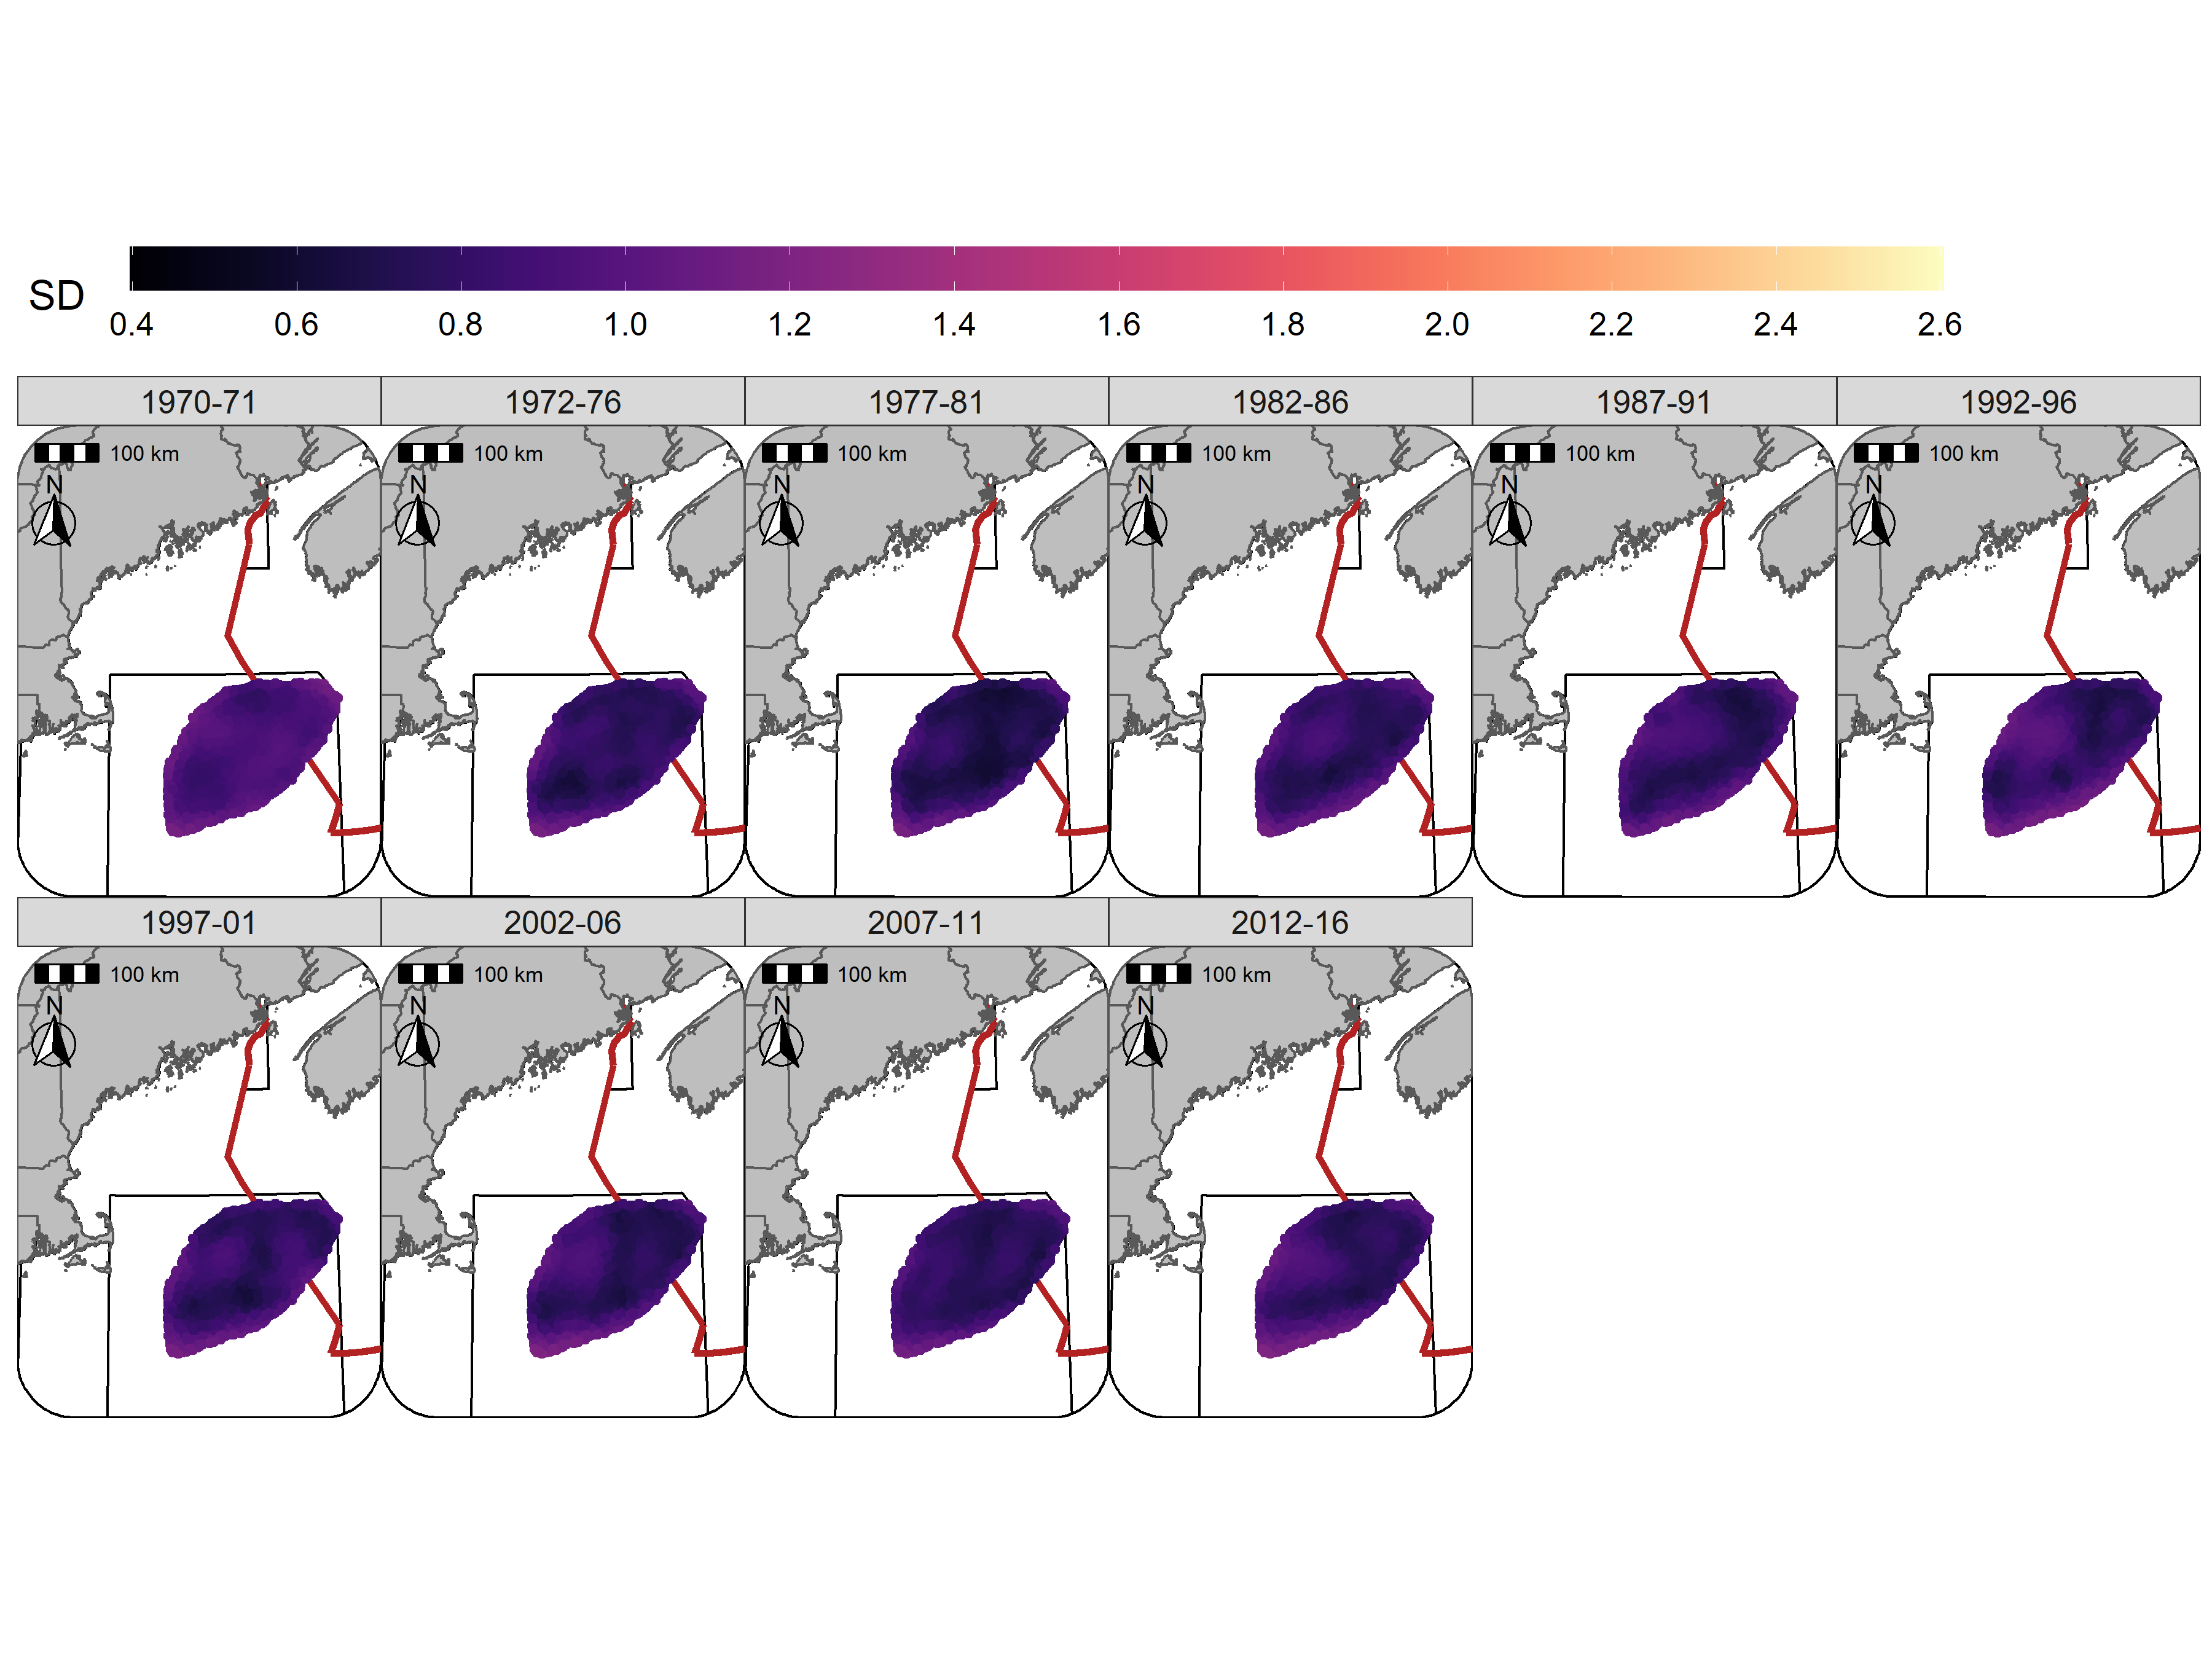
\includegraphics[width=1\linewidth]{D:/Github/Paper_2_SDMs/Results/Figures/rf_fall_yt_sd} \caption{Standard deviation of random fields (logit scale) for Yellowtail Flounder in each era during the Fall (NMFS-fall survey) using the SST + Dep + Sed model and 5-year random field.}\label{fig:rf-fall-yt-sd}
\end{figure}
\end{landscape}

\hypertarget{hyperparameters}{%
\subsection{Hyperparameters}\label{hyperparameters}}

For Atlantic Cod, the estimate for the variance of the Dep variance hyperparameter was highest in Winter and declined through to the Fall, reflecting the decline in the influence of this covariate in the Fall (Figure \ref{fig:hyper-dep-var-est}). For Yellowtail Flounder, the variance of the Dep hyperparameter was higher than observed for Atlantic Cod throughout the year and reflected the relative stability in the effect size of this covariate throughout the year (Figure \ref{fig:hyper-dep-var-est}). The SST variance hyperparameter for Atlantic Cod was relatively stable throughout the year and reflects the consistent influence of the SST covariate on the distribution of cod. For Yellowtail Flounder, the SST variance hyperparameter was relatively low throughout the year and aligns with the consistent small effect of the SST covariate on the distribution of Yellowtail Flounder (Figure \ref{fig:hyper-sst-var-est}). The uncertainty of these estimates precludes any statistical differences being observed between the seasons.

\begin{figure}
\includegraphics[width=1\linewidth]{D:/Github/Paper_2_SDMs/Results/Figures/hyper_dep_var_est} \caption{Dep variance hyperparameter estimate with 95\% credible intervals for each stock in each season.}\label{fig:hyper-dep-var-est}
\end{figure}

\clearpage

\begin{figure}
\includegraphics[width=1\linewidth]{D:/Github/Paper_2_SDMs/Results/Figures/hyper_sst_var_est} \caption{SST variance hyperparameter estimate with 95\% credible intervals for each stock in each season.}\label{fig:hyper-sst-var-est}
\end{figure}

\clearpage

\begin{figure}
\includegraphics[width=1\linewidth]{D:/Github/Paper_2_SDMs/Results/Figures/cod_winter_marginal} \caption{Posteriors distributions of the four model hyperparameters for Atlantic Cod in the Winter.}\label{fig:hyper-cod-winter-post}
\end{figure}

\clearpage

\begin{figure}
\includegraphics[width=1\linewidth]{D:/Github/Paper_2_SDMs/Results/Figures/cod_spring_marginal} \caption{Posteriors distributions of the four model hyperparameters for Atlantic Cod in the Spring.}\label{fig:hyper-cod-spring-post}
\end{figure}

\clearpage

\begin{figure}
\includegraphics[width=1\linewidth]{D:/Github/Paper_2_SDMs/Results/Figures/cod_fall_marginal} \caption{Posteriors distributions of the four model hyperparameters for Atlantic Cod  in the Fall.}\label{fig:hyper-cod-fall-post}
\end{figure}

\clearpage

\begin{figure}
\includegraphics[width=1\linewidth]{D:/Github/Paper_2_SDMs/Results/Figures/yt_winter_marginal} \caption{Posteriors distributions of the four model hyperparameters for Yellowtail Flounder in the Winter.}\label{fig:hyper-yt-winter-post}
\end{figure}

\clearpage

\begin{figure}
\includegraphics[width=1\linewidth]{D:/Github/Paper_2_SDMs/Results/Figures/yt_spring_marginal} \caption{Posteriors distributions of the four model hyperparameters for Yellowtail Flounder in the Spring.}\label{fig:hyper-yt-spring-post}
\end{figure}

\clearpage

\begin{figure}
\includegraphics[width=1\linewidth]{D:/Github/Paper_2_SDMs/Results/Figures/yt_fall_marginal} \caption{Posteriors distributions of the four model hyperparameters for Yellowtail Flounder in the Fall.}\label{fig:hyper-yt-fall-post}
\end{figure}

\clearpage

\end{document}
